\documentclass[12pt,PhD,oneside,leqno]{muthesis}

%\addtolength{\oddsidemargin}{-1in}
%\addtolength{\evensidemargin}{-1in}

% TODO: change to TWOSIDE later and remove the addtolength!
% The regulations say that 12pt should be used
% Change the MSc option to MPhil, MRes or PhD if appropriate

%\usepackage[round]{natbib}

%colours!
\usepackage{color}
\definecolor{lbcolor}{rgb}{0.9,0.9,0.9}
\definecolor{darkblue}{rgb}{0,0.08,0.45}


% some standard packages
\usepackage{textcomp}
\usepackage{gensymb}
\usepackage{tabularx}
\usepackage{setspace}
\usepackage{xspace}
\usepackage{verbatim}
\usepackage{graphicx}
\usepackage{caption}


\usepackage{subcaption}
\usepackage{url} 


\usepackage{multirow} 
\usepackage{booktabs}

% correct quotation marks for british english
\usepackage[english]{babel}
\usepackage[english=british]{csquotes}

% nice list formatting. neveradjust option is needed to always indent items in compactitem/compactenum
\usepackage[neveradjust]{paralist}
%\usepackage[shortlabels]{enumitem}


%symbols
\usepackage{amssymb,amsmath}

\usepackage[savemem]{listings}
\lstloadlanguages{C++, XML}
\lstset{language=XML,
	captionpos=b,
	numbers=left,
    stepnumber=1,
	numbersep=5pt,
	numberstyle=\footnotesize,
	breaklines=true,
	breakautoindent=true,
	postbreak=\space,
	tabsize=2,
	basicstyle=\ttfamily\small,
	showspaces=false,
	showstringspaces=false,
	extendedchars=true,
	xleftmargin=0.5cm,
	backgroundcolor=\color{lbcolor}}

% Uncomment the following lines if you want to include the date as a
% header in draft versions
%\usepackage{fancyhdr}
%\pagestyle{fancy}
%\lhead{}  % left head
%\chead{Draft: \today} % centre head
%\lfoot{}
%\cfoot{\thepage}
%\rfoot{}
%\fancypagestyle{plain}{%
%	\fancyhead{}%
%	\renewcommand{\headrulewidth}{0pt}%
%}

%\renewcommand{\sectionmark}[1]{\markright{\thesection\ #1}}
%\fancyhf{}
%\fancyhead[RO]{\sffamily\bfseries\thepage}
%\fancyhead[LO]{\sffamily\bfseries\rightmark}
%\addtolength{\headheight}{5pt}
%\renewcommand{\headrulewidth}{0.5pt}
%\renewcommand{\footrulewidth}{0pt}

% style for empty pages
%\fancypagestyle{plain}{%
%	\fancyhead{}%
%	\renewcommand{\headrulewidth}{0pt}%
%}

\usepackage[%
	pdftitle={The Justificatory Structure of OWL Ontologies},%
	pdfauthor={Samantha Patricia Bail},%
	pdfsubject={The Justificatory Structure of OWL Ontologies},%
	pdfkeywords={OWL, semantic web, ontologies, explanation},%
	hyperfootnotes=true,
	backref=page]{hyperref}

\hypersetup{colorlinks=true,%
	citecolor=black,%
	filecolor=black,%
	linkcolor=black,%
	urlcolor=black}
	
\renewcommand*{\backref}[1]{}
\renewcommand*{\backrefalt}[4]{%
    \ifcase #1 (Not cited.)%
    \or        (Cited on page~#2.)%
    \else      (Cited on pages~#2.)%
    \fi}

% Uncomment the next line if you want subsubsections to be numbered
%\setcounter{secnumdepth}{3}
% Uncomment the next line if you want subsubsections to appear in
% the table of contents
%\setcounter{tocdepth}{4}


%% for adding notes in right margin - remove in final version!

\usepackage[
	textwidth=10em, 
	colorinlistoftodos, 
	backgroundcolor=yellow!70,
	linecolor=yellow!70, 
	bordercolor=white]
	{todonotes}
	

% begin / end environments
\usepackage{amsthm}
\newtheorem{thm}{Theorem}[chapter]
\newtheorem{prop}{Proposition}[chapter]
\newtheorem{cor}{Corollary}[chapter]
\newtheorem{defn}{Definition}[chapter]
\newtheorem{examp}{Example}[chapter]
\newtheorem{rmk}{Remark}[chapter]

\usepackage{owl}  % for DL names - not guaranteed to work in all cases :)

\usepackage{tikz}
\usetikzlibrary{shapes,positioning}

\usepackage{algorithmicx}
\usepackage{algpseudocode}
\usepackage[chapter]{algorithm}
\usepackage{graphviz}

\newcommand{\sdev}{\ensuremath{\sigma}\xspace}
\newcommand{\median}{\ensuremath{m}\xspace}
\newcommand{\entsetstar}{\ensuremath{\varepsilon^{*}}\xspace}

\newcommand{\modif}{\ensuremath{mod}\xspace}
\newcommand{\setcard}[1]{\ensuremath{ \left|{#1}\right|}\xspace}
\newcommand{\oprime}{\ensuremath{\mathcal{O'}}\xspace}
\newcommand{\jprime}{\ensuremath{\mathcal{J'}}\xspace}

\usepackage{pifont}% http://ctan.org/pkg/pifont
\newcommand{\cmark}{\ding{51}}%
\newcommand{\xmark}{\ding{55}}%

%\usepackage{datatool}
%\usepackage{lscape}
%\usepackage{longtable}

%\DTLsetseparator{,}
%\DTLloaddb{testfile}{tests/testfile2.csv}

%\renewcommand{\dtldisplaystarttab}{\hline}
%\renewcommand{\dtldisplayendtab}{\\ \hline}
%\renewcommand{\dtldisplayafterhead}{\hline}

\newcommand{\deltaiac}{\ensuremath{\bigtriangleup^{I_{ac}}}\xspace}
\newcommand{\deltaia}{\ensuremath{\bigtriangleup^{I_{a}}}\xspace}
\newcommand{\dotiac}{\ensuremath{\cdot^{I_{ac}}}\xspace}
\newcommand{\dotia}{\ensuremath{\cdot^{I_{a}}}\xspace}

% changes equation numbering to be single numbers - good for axiom sets	
\renewcommand{\theequation}{\arabic{equation}}

\usepackage{tabu}
\tabulinesep=1mm

%\usepackage{mathtools}

%\usepackage[a4paper,bottom=1.5in]{geometry}

\usepackage{titlesec}
\titlespacing*{\chapter}{0pt}{-20pt}{30pt}
\titleformat{\chapter}[display]{\normalfont\huge\bfseries}{\chaptertitlename\ \thechapter}{20pt}{\Huge}

\usepackage{rotating}


%\renewcommand{\thesubfigure}{\thechapter.\arabic{figure}\alph{subfigure}}



% Uncomment the next line if you want subsubsections to be numbered
%\setcounter{secnumdepth}{3}
% Uncomment the next line if you want subsubsections to appear in
% the table of contents
\setcounter{tocdepth}{2}


\begin{document}
% Uncomment the following lines to leave out list of figures, tables
% and copyright until final printing
%\figurespagefalse
%\tablespagefalse
%\copyrightfalse

\title{The Justificatory Structure\\ of OWL Ontologies}
\author{Samantha Patricia Bail}
%\principaladviser{Supervisor: Bijan Parsia and Ulrike Sattler}
%\firstreader{First reader}

\beforeabstract

\prefacesection{Abstract}
%\abstracttitle
The Web Ontology Language OWL is based on the highly expressive description logic \dl{SROIQ}, which allows OWL ontology users to employ out-of-the-box reasoners to compute information that is not only explicitly asserted, but \emph{entailed} by the ontology. \emph{Explanation} facilities for entailments of OWL ontologies form an essential part of ontology development tools, as they support users in detecting and repairing errors in potentially large and highly complex ontologies, thus helping to ensure ontology quality. 

\emph{Justifications}, minimal subsets of an ontology that are sufficient for an entailment to hold, are currently the prevalent form of explanation in OWL ontology development tools, and they have been found to significantly reduce the time and effort required to debug erroneous entailments. A large number of entailments, however, have not only one but \emph{many} justifications, which can make it considerably more challenging for a user to find a suitable repair for the entailment.

In this thesis, we investigate the relationships between multiple justifications for both single and multiple entailments, with the goal of exploiting this \emph{justificatory structure} in order to devise new \emph{coping} strategies for multiple justifications. We describe various aspects of the justificatory structure of OWL ontologies, such as shared axiom cores and structural similarities. We introduce a model for measuring user effort in the debugging process and propose debugging strategies that exploit the justificatory structure in order to reduce user effort. Finally, an analysis of a large corpus of ontologies from the biomedical domain reveals that OWL ontologies used in practice frequently exhibit a rich justificatory structure.

\bigskip 

\noindent Date of submission: 26/04/2013
\afterabstract

%\prefacesection{Acknowledgements}
%I would like to thank my supervisors Bijan Parsia and Uli Sattler for their support, enthusiasm, and incredible patience with me throughout this PhD. I would also like to thank the \emph{DL-istas} in the IMG and BHIG for their ideas and the many interesting ad-hoc discussions in our office, in particular Colin Puleston who dedicated his time to saving my broken code. And finally, I want to thank my family who have been so supportive over the course of my seemingly never-ending studies.
%\afterpreface


\chapter{Introduction}
\label{chap:introduction}

Since its standardisation by the W3C in 2004, the Web Ontology Language OWL \cite{w3c09eu} has become a widely used language for representing ontological knowledge. OWL ontologies are used across a wide spectrum of domains, ranging from chemistry to bio-health informatics and medical data. In its latest version, OWL 2 \cite{cuenca-grau08kw}, which is based on the expressive description logic \dl{SROIQ} \cite{dlhb03,horrocks06ya}, allows ontology modellers to use highly complex expressions to describe the entities in an ontology. 

An OWL ontology is a set of \emph{axioms}, which make statements about the classes, properties, and individuals in an ontology, as well as the relations between them. Due to its foundations in description logics \cite{dlhb03} and the availability of highly optimised description logic reasoners, OWL ontology modellers and users can apply automated reasoning techniques to elicit not only explicitly asserted knowledge in the ontology, but also \emph{implicit} information which is \emph{entailed} by the ontology. This makes it possible to model complex hierarchical relations  without the need to make explicit every single relation between sub- and super-classes. For example, an ontology which contains the axioms \ax{Cat \subcls Carnivore} (\enquote{every \cn{Cat} is a \cn{Carnivore}}) and \ax{Carnivore \subcls Animal} (\enquote{every \cn{Carnivore} is an \cn{Animal}}) also entails the statement \ax{Cat \subcls Animal}, without having to explicitly state it.

Ontology development often resembles traditional software development: from the first design to a release candidate, axioms and entities are frequently added, modified, and removed. Some OWL ontologies, such as the National Cancer Institute (NCI) Thesaurus ontology \cite{coronado04zh}, undergo a highly dynamic iterative development process, with a team of developers working to produce monthly updates of the ontology. As ontology re-use and sharing on the web is highly encouraged, existing OWL ontologies may be imported, or merged into newly built ones. OWL editing tools, such as the \protege editor,\footnote{\url{http://protege.stanford.edu/}} allow ontology developers to create large and complex ontologies; we often find OWL ontologies that contain thousands of classes and axioms which are highly interlinked across the ontology \cite{wang06rr,horridge11ac}. 

All these processes can lead to \emph{errors} in the resulting ontology. The two classes of commonly occurring errors in OWL ontologies are unwanted entailments and unwanted \emph{non}-entailments. Among the former, \emph{incoherence} and \emph{inconsistency} of an ontology can be detected automatically, as they have distinguishing logical features while also being reliably connected to errors. Incoherence refers to the presence of an \emph{unsatisfiable} class in the ontology, that is, a class which cannot have any instances, while \emph{inconsistency} of the ontology means that the ontology does not have any meaningful entailments at all. Similar to the debugging process in software development, the \emph{repair} of such errors involves finding those parts of the ontology that cause the problem, then modifying or removing them in order to rectify the error. 

Due to the large size and often complex structure of OWL ontologies, finding and repairing these errors without appropriate tool support can be daunting and error-prone: simply removing those parts of the ontology which are suspected to cause the error may result in a significant loss of \emph{relevant} information but is not guaranteed to sufficiently repair the ontology. This is where \emph{explanation} comes into play: on an abstract level, an explanation for an entailment of an ontology is a statement, or a set of statements, which traces the source of the error and \emph{explains} to the user \emph{what} information in the ontology lead to the entailment and \emph{how} it does this. 

Explanation has a long history in the research on intelligent systems (e.g.\ \cite{clancey81mg,buchanan84zb}). It has been considered an important component of expert systems, such as MYCIN \cite{buchanan84lq}, since the early 1980s, not just for the purpose of \emph{debugging} a system, but also for tasks such as learning about the information modelled in the system, and convincing human experts of the system's correctness. Because of its role in these tasks, explanation is thought to enhance both the correctness and the acceptance of an intelligent system. Russell and Norvig \cite{russell03aa} illustrate this point with an example of the role explanation facilities play in user-facing expert systems:

\begin{quote}
\emph{\enquote{A leading expert on lymph-node pathology describes a fiendishly difficult case to the expert system, and examines the system's diagnosis. He scoffs at the system's response. Only slightly worried, the creators of the system suggest he ask the computer for an explanation of the diagnosis. The machine points out the major factors influencing its decision and explains the subtle interaction of several of the symptoms in this case. The experts admits his error, eventually.}}
\end{quote}

Explanation can assume various forms, such as a trace of rules in rule-based expert systems \cite{buchanan84lq}, or proofs in logic-based systems \cite{borgida99cn,mcguinness96rp}. In OWL tools, explanation generally takes the form of a \emph{pinpoint} of the set---or sets---of axioms that cause the entailment to hold, which we commonly denote as \emph{justifications}. 

\section{Justification-based debugging support}

Justification-based explanation support for description logic ontologies is the most prevalent form of explanation in current OWL development tools, with OWL editors such as \protege and \swoop\footnote{\url{https://code.google.com/p/swoop/}} providing justification-based debugging tools. There exists a large body of research from the past decade which underlines the important role justification-based explanations play in the ontology development process (e.g.\ \cite{schlobach03nc,kalyanpur05mi,lam07aa,horridge08yi}).

A justification \just for an entailment \ent of an ontology \ont is a minimal subset of \ont which is sufficient for \ent to hold. Justifications have two major benefits: first, the minimality of a justification prevents the tedious process of searching through the ontology in order to find the responsible axioms, while also allowing users to focus on a (usually) small subset of the ontology. And second, since a justification simply consists of axioms occurring in \ont, ontology developers do not have to learn any additional mechanisms or notations in order to understand the explanation. The following example illustrates the idea of justification-based debugging support:
\begin{examp}
~\newline ~\newline
\small
\begin{tabu}{rlrl}
		(1)&\ax{Cat \subcls Carnivore} &(5)&\ax{PetOwner \eqcls Human\conj \exists hasPet.Animal}\\
		(2)&\ax{Carnivore \eqcls Animal \conj \forall eats.Animal}& (6)&\ax{Cat \subcls \exists eats.Mouse}\\
		(3)&\ax{Plant \subcls \lnot Animal}	&(7)&\ax{SickCat \equiv Cat \conj \exists eats.Grass}\\
		(4)&\ax{Grass \subcls Plant} & (8)&\ax{\exists eats.\thing \subcls Animal}
\end{tabu}
\end{examp}

The ontology \O comprising the axioms in the above example makes statements about the entities in the domain of animals and their eating habits.\footnote{For the purpose of this example, we assume the statement \ax{\exists eats.\thing \subcls Animal} to be correct.} Several other statements follow logically from \O, for example \ax{Cat \subcls Animal} (\enquote{everything that is a \cn{Cat} is an $\mathsf{Animal}$}) and the unsatisfiability of the concept \cn{SickCat}, which is expressed as \cn{SickCat \subcls \bot}. In ontology development tools, such unsatisfiable concepts are usually highlighted to make the user aware of them, for example by rendering them in red colour, or arranging them as a sub-concept of \cn{Nothing}. 

Unsatisfiable classes are commonly regarded as errors, as they cannot have any instances. An ontology developer would want to repair the error by re-writing or removing some of the axioms responsible for causing it. Without a debugging tool, the user has to browse the ontology, find the responsible axioms, and apply modifications they consider appropriate. Providing a justification for the entailment, however, allows the user to focus directly on the responsible axioms, thus clearly reducing the effort involved in finding a suitable repair---and preventing the user from going down the \enquote{wrong path} or giving up their search for the \enquote{needle in the haystack}. 

In our example ontology, there exists exactly one justification for the entailment \cn{SickCat \subcls \bot}, namely the set consisting of the axioms \ax{Cat \subcls Carnivore}, \ax{Carnivore \eqcls Animal \conj \forall eats.Animal},  \ax{Grass \subcls Plant}, \ax{SickCat \eqcls Cat \conj \exists eats.Grass}, \\and \ax{Plant \subcls \lnot Animal}. The contradiction stems from the fact that \cn{Cat} is asserted to be an animal which only eats other animals, but \cn{SickCat} eats \cn{Grass}, which is asserted to be a \cn{Plant}, thus not an \cn{Animal}. There are different approaches to repairing this error, such as weakening the restriction that a \cn{Carnivore} eats \emph{only} \cn{Animals}; however, as we can already see from this small example, finding an appropriate repair without weakening or sacrificing too much information is a non-trivial task and requires the user to understand the relations between the axioms in the justification.

\subsection{Understanding justifications}

Repairing an entailment becomes more challenging as the number of justifications for an entailment grows. Given the entailment \ax{Cat \subcls Animal} from the above ontology in example, we can find two justifications: the set consisting of the two axioms \ax{Cat \subcls Carnivore} and \ax{Carnivore \eqcls Animal \conj \forall eats.Animal}, and the second, perhaps less obvious, justification containing \ax{Cat \subcls \exists eats.Mouse} and \ax{\exists eats.\thing \subcls Animal}. A user who wants to understand why \ax{Cat \subcls Animal} follows from the ontology will be presented with both justifications; if this entailment was unwanted, the user would have to understand and break \emph{both} justifications in order to remove it from the ontology. 

Assume the user is faced not only with a small toy ontology as the one above, but with a large and complex ontology, containing several thousand classes, properties, individuals, and axioms. The number of justifications for a single entailment can grow exponentially in the number of axioms in the ontology, with several thousand found in some ontologies used in practice \cite{bail11jm}. And still, if the user wants to ensure the entailment does no longer hold in the ontology, every single justification has to be broken. While it is possible for a user to inspect and modify every justification in isolation, this approach is time-consuming and error-prone. What we need is a strategy that helps users \emph{cope} with multiple justifications and supports them in finding an appropriate repair.

The question of how users \emph{interact} with justifications once they have been computed has been receiving some attention over the past few years \cite{kalyanpur06fj,lam06tk,horridge10gs,horridge11gj}. Depending on the respective task, whether the explanation is requested to fix an error or to aid understanding of an entailment, this interaction can assume different shapes and objectives. For the purpose of debugging, users may regard a \emph{minimal repair} as crucial, that is, removing an error while losing as little other information as possible. This may be achieved by modifying the given justifications to make them easier to understand to users, or, when dealing with multiple justifications, by identifying axioms which occur across several justifications.

In case of the former, \emph{fine-grained} justifications \cite{lam06tk,kalyanpur06fj,horridge08yi} are variants of justifications which are as weak as possible and do not contain any superfluous expressions that could possibly distract a user from the actual cause of the entailment. Such fine-grained justifications have been defined more precisely as \emph{laconic} and \emph{precise} justifications \cite{horridge08yi}, with suitable and efficient algorithms to compute them for entailments of OWL ontologies. In the above example, the justification \{\ax{Cat \subcls Carnivore}, \ax{Carnivore \eqcls Animal \conj \forall eats.Animal}\!\!\} for the entailment \ax{Cat \subcls Animal} can be re-written into its laconic version \{\ax{Cat \subcls Carnivore}, \ax{Carnivore \subcls Animal}\!\!\}, which reduces the second axiom to its \emph{relevant} parts. While fine-grained justifications might make it easier to understand a single justification, they do not support understanding multiple justifications for an entailment.

Dealing with multiple justifications, either for individual or for \emph{multiple entailments}, has been somewhat facilitated by the introduction of \emph{root and derived} justifications \cite{parsia05dg} which assist in the repair of multiple unsatisfiable classes: a root justification is a subset of a derived justification; fixing the root justification also repairs all those justifications which are derived from it. As an example, assume we add the axiom \ax{SickCatOwner \eqcls PetOwner \conj \exists hasPet.SickCat} to the ontology. The class \cn{SickCatOwner} will then be unsatisfiable, but its unsatisfiability depends entirely on the unsatisfiabilty of the class \cn{SickCat}. Thus, \cn{SickCatOwner} is a derived unsatisfiable class, whereas \cn{SickCat} is the root cause. Root and derived justifications, as used in the ontology editor \swoop, have been successfully shown to reduce user effort when debugging multiple entailments \cite{kalyanpur05mi}. 

\subsection{Justificatory structure}

The debugging tool in the \swoop editor by Kalyanpur was the first attempt to make use of the \emph{relations} between justifications in order to support the user in finding a suitable repair for multiple justifications. In addition to root and derived information, the repair tool also presents metrics for the axioms in the justifications, such as the axiom frequency (the number of justifications an axiom occurs in), impact (the number of entailments an axiom affects), and usage (of terms occurring in the axiom). Based on these metrics, the tool computes a rank for each axiom, with the lowest ranked axioms being suggested for removal or modification. This provides users with important guidance on where to start repairing a set of justifications.

This approach makes use of the fact that there exist structural relations between justifications, such as shared axioms of various extents, ranging from single axioms to subset relationships, as in the case of root and derived justifications. In other words, given a set of entailments of an ontology and their justifications, we can identify the \emph{justificatory structure} of the ontology, that is, the set of features and relations of its justifications. 

Despite the potential usefulness for improving debugging support for multiple justifications and the insights we can gain into the relationships between entailments of OWL ontologies, their justifications, and the axioms they contain, there has been no further exploration of the justificatory structure of OWL ontologies. Therefore, one of the main goals of this thesis is to identify the different aspects of justificatory structure of ontologies, to investigate potential applications of these relations in the debugging process, and to establish how prevalent these structural aspects are in OWL ontologies used in practice.

Shared axiom relationships, such as root and derived justifications, are only one aspect of justificatory structure. Another interesting phenomenon we often find in OWL justifications is the \emph{similarity} between justifications, as we can see in the well-known \emph{Pizza} tutorial\footnote{\url{http://owl.cs.manchester.ac.uk/tutorials/protegeowltutorial/}} ontology: take, for example, the entailment \ax{Fiorentina \subcls InterestingPizza}, which has over 200 justifications. The following example shows three of those justifications; \cn{Fiorentina} is abbreviated to \cn{Fi}, \cn{hasTopping} to \cn{hasTop}, \cn{InterestingPizza} to \cn{IP}, and \thing is the description logic notation for the top concept \cn{Thing} which stands for \enquote{any element in the domain}.
\begin{examp}
~\newline ~\newline
\footnotesize
\begin{tabu}{rlll}
(1) & \ax{Fi \subcls NamedPizza} &  \ax{Fi \subcls NamedPizza } &  \\
(2) &\ax{NamedPizza \subcls Pizza} &  \ax{NamedPizza \subcls Pizza} &   \ax{domain(hasTop, Pizza)} \\
(3) &\ax{Fi \subcls \exists hasTop.Tomato} &  \ax{Fi \subcls \exists hasTop.Tomato} &   \ax{Fi \subcls \exists hasTop.Tomato} \\
(4) &\ax{Fi \subcls \exists hasTop.Olive} &  \ax{Fi \subcls \exists hasTop.Mozzarella} &  \ax{Fi \subcls \exists hasTop.Garlic} \\
(5) &\ax{Fi \subcls \exists hasTop.Spinach} &   \ax{Fi \subcls \exists hasTop.Olive} &    \ax{Fi \subcls \exists hasTop.Spinach} \\
(6) &\ax{Spinach \subcls \neg Tomato} &   \ax{Mozzarella \subcls \neg Tomato }&   \ax{Spinach \subcls \neg Tomato} \\
(7) &\ax{Spinach \subcls \neg Olive} &   \ax{Mozzarella \subcls \neg Olive} &    \ax{Spinach \subcls \neg Garlic} \\
(8) &\ax{Olive \subcls \neg Tomato} &   \ax{Olive \subcls \neg Tomato} &   \ax{Garlic \subcls \neg Tomato}   \\
(9) &\ax{IP \eqcls Pizza \conj \geq 3 hasTop.\thing}  &  \ax{IP \eqcls Pizza \conj \geq 3 hasTop.\thing} &  \ax{IP \eqcls Pizza \conj \geq 3 hasTop.\thing} 
\end{tabu}
~\newline
\end{examp}

While these justifications may look complicated at first, they can all be easily summarised as follows:
\begin{compactitem}
\item Axioms 1-2 (2-3 in the last justification): \cn{Fiorentina} is a \cn{Pizza}.
\item Axioms 3-5: \cn{Fiorentina} has three kinds of toppings.
\item Axioms 6-8: These three toppings are pairwise disjoint, that is, no element in the domain can be a member of several toppings at the same time.
\item Axiom 9: Anything that is a \cn{Pizza} and has at least three toppings is an \cn{InterestingPizza}.
\end{compactitem}

Despite the fact that the justifications contain different axioms, we can immediately see that they are very similar and that it suffices to understand the reasoning in the abstract explanation in order to understand the concrete examples. Since \cn{Fiorentina} is defined to have six different toppings, the justifications for \ax{Fiorentina \subcls InterestingPizza} are all combinations of three toppings, variations on the reasons why these toppings are pairwise disjoint, and variations of the reasons why \cn{Fiorentina} is a \cn{Pizza}. 

This adds another goal to our investigation of justificatory structure: to determine a set of equivalence relations that allow us to identify such structural similarities, and to investigate how prevalent these similarities are in OWL ontologies---or whether the \emph{Pizza} ontology is just a unique case. The presence of structural similarity provides us with a starting point for lifting justifications from their material form to an abstract explanation \emph{template}, which could drastically reduce the cost of understanding the logical structure of each individual justification. This, in turn, reduces the overall effort a user has to apply in order to debug an entailment with multiple structurally similar justifications.


\subsection{Beyond debugging and repair}

While we put strong emphasis on the debugging aspect of justifications, we may also consider their suitability for other purposes in the ontology development process. In the same way as explanation in expert system serves multiple purposes, we can use justifications in OWL ontologies for tasks beyond debugging, such as ontology comprehension and exploration, ontology learning, and generating ontology metrics.

\emph{Ontology comprehension} \cite{keet07pc,bauer09ru} describes the process of a person understanding what knowledge is modelled in an ontology and how it is modelled; this is of particular relevance to users attempting to use or integrate an existing ontology. We believe that examining a set of entailments and their justifications can help users gain insights into the relations between the pieces of information contained in the ontology, thus enhancing their understanding of the ontology. Going back to the \emph{Pizza} example above, we can see that by inspecting only a small number of justifications and their abstract template, we already have some understanding of the basic reasoning behind \emph{all} classes in the ontology which are entailed to be an \cn{InterestingPizza}.

Another potentially useful application of justifications is \emph{ontology metrics}: ontology editors commonly display a set of metrics of an ontology, such as the number and types of axioms, the number of entailments, and the logical expressivity based on the constructors used in the ontology. These ontology metrics allow users to infer information about the size and complexity of the ontology, its \emph{richness} of modelling (that is, the level of detail used to describe a class), and even its general quality \cite{tartir05im,alani06or}. Justification-based metrics, such as the numbers of justifications per entailments, the relations between them, and their structural similarities, add another layer to the existing suite of ontology metrics. These metrics can be used to compare the quality, uniformity, and \enquote{interestingness} of ontologies based on their modelling.


\section{Research objectives}

In summary, the main goals of this thesis are to explore the notion of  \enquote{justificatory structure} of OWL ontologies, to investigate the landscape of justificatory structure in ontologies used in practice, and to suggest approaches to using the justificatory structure in order to reduce user effort in the ontology debugging process.

First, we aim to gain a clearer understanding of the landscape of justifications in OWL ontologies. Our goal is to determine how prevalent multiple justifications are in OWL ontologies and what shapes (size, axiom types) these justifications commonly assume. We want to identify a set of relations between justifications which go beyond root and derived unsatisfiable classes, taking into account both shared axioms and shared axiom sets between justifications. 

This includes structural similarities between justifications: we want to find a (reasonable) set of equivalence relations that allow us to capture similarities between justifications and group them based on their abstract explanation templates. Taking these relations, we want to know whether they commonly occur in OWL ontologies found \enquote{in the wild} and how prevalent they are in order to see how effectively they can be used to \emph{summarise} multiple justifications.

Second, we look at justificatory structure in order to address the problem of coping with multiple justifications in a debugging and repair scenario. We first need to pin down the basic notion of \emph{effort} required to solve a debugging task involving multiple justifications before we can identify ways of exploiting the justificatory structure in order to reduce the effort ontology users have to spend when debugging one or multiple entailments.


\section{Contributions}

\begin{compactitem}
\item We provide a set of design decisions for computing finite sets of entailments of OWL ontologies and discuss the benefits and drawbacks of the various options. This has practical implications for the display of \emph{selected entailments} in OWL editors and for the use of entailments as a measure of the information content in ontologies. It also informs the generation and analysis of justifications for finite entailment sets in the context of this thesis.

\item We introduce the notion of the justificatory structure of OWL ontologies which allows us to characterise structural relations between justifications for both single and multiple entailments. This includes the characterisation of various aspects of justificatory structure, such as justification properties, axiom properties, and axiom overlap between justifications.

\item We introduce two equivalence relations between justifications, subexpression-isomorphism and lemma-isomorphism, which are used to analyse the logical diversity of a set of justifications. These equivalence relations partition a set of justifications, with equivalent justifications following the same lines of reasoning. This provides the foundations for representing a set of justifications by an abstract justification \emph{template} which summarises a set of justification, thus reducing the effort involved in understanding multiple justifications.

\item We pin down the notion of a \emph{debugging problem} and present a model of measuring \emph{effort} for successfully solving debugging problems using justifications. We then propose strategies to exploit the justificatory structure of a set of justifications in order to reduce user effort when dealing with multiple justifications.

\item Finally, we present the results of a survey of the justificatory structure of OWL ontologies from the NCBO Bioportal. We find that a large number of OWL ontologies in the test corpus exhibit a very rich justificatory structure, with frequently occurring multiple justifications, high extents of overlaps, and high-frequency axioms. Using the newly introduced equivalence relations, we find that the logical diversity of OWL justifications is significantly lower than their numbers may indicate, with justification sets being reduced to only 10\% of their original size.


\end{compactitem}


\section{Published Work}
Some of the work presented in this thesis has been published at peer-reviewed conferences and workshops. The following publications correspond roughly to chapters 3 (reference 1), 4 (reference 2-3), 5 (reference 4-5), and 6 (reference 6-8) in this thesis:

\begin{compactenum}

\item \cite{bail11kk} Samantha Bail, Bijan Parsia, and Ulrike Sattler. Extracting finite sets of entailments from OWL ontologies. In \emph{Proceedings of the 24th International Workshop on Description Logics (DL-11)}, 2011.

\item \cite{bail10kb} Samantha Bail, Bijan Parsia, and Ulrike Sattler. The justificatory structure of OWL ontologies. In \emph{Proceedings of the 7th International Workshop on OWL: Experiences and Directions (OWLED-10)}, 2010.

\item \cite{bail11jm} Samantha Bail, Matthew Horridge, Bijan Parsia, and Ulrike Sattler. The justificatory structure of the NCBO Bioportal ontologies. In \emph{Proceedings of the 10th International Semantic Web Conference (ISWC-11)}, 2011.

\item \cite{bail12aa} Samantha Bail, Bijan Parsia, and Ulrike Sattler. Diversity of reason: Equivalence relations over description logic explanations. In \emph{Proceedings of the 25th International Workshop on Description Logics (DL-12)}, 2012.

\item \cite{bail12ab} Samantha Bail, Bijan Parsia, and Ulrike Sattler. Declutter Your Justifications: Determining Similarity Between OWL Explanations. In \emph{Proceedings of the First International Workshop on Debugging Ontologies and Ontology Mappings (WoDOOM-12)}, 2012.

\item \cite{horridge11si} Matthew Horridge, Samantha Bail, Bijan Parsia, and Ulrike Sattler. The cognitive complexity of OWL justifications. In \emph{Proceedings of the 24th International Workshop on Description Logics (DL-11)}, 2011.

\item \cite{horridge11gj} Matthew Horridge, Samantha Bail, Bijan Parsia, and Ulrike Sattler. The cognitive complexity of OWL justifications. In \emph{Proceedings of the 10th International Semantic Web Conference (ISWC-11)}, 2011.

\item \cite{horridge13aa} Matthew Horridge, Samantha Bail, Bijan Parsia, and Ulrike Sattler. Toward cognitive support for OWL justifications. \emph{Submitted to: Knowledge-Based Systems}, 2013.

\end{compactenum}





\chapter{Background and related work}
\label{chap:background}

Knowledge representation (KR) is an area of artificial intelligence research which deals with representing knowledge using  symbols, thus allowing the application of automated reasoning techniques to infer new knowledge from given knowledge \cite{brachman2004aa}. KR forms the basis of \emph{knowledge-based systems}, \enquote{intelligent} systems which make use of a \emph{knowledge base} (KB) that contains told facts about some domain, as well as procedures to reason over these facts and infer implicit knowledge. While there exists a wide range of approaches to implementing knowledge-based systems, such as logic programming \cite{baral94aa}, frames \cite{minsky74aa}, and semantic networks \cite{sowa87st}, in this thesis we are dealing with description logics (DLs) \cite{dlhb03} as the underlying knowledge representation formalism for knowledge bases. DLs are a family of logics based on a guarded fragment of first-order logic which is more expressive than propositional logic, while still being decidable \cite{dlhb03}.

This chapter introduces the basic concepts of description logics, which underpin the Web Ontology Language OWL \cite{horrocks03vn,cuenca-grau08kw}. It outlines the syntax and semantics of description logics and fixes relevant notions such as \emph{axioms} and \emph{entailments} of an OWL ontology. It also discusses the landscape of logical and non-logical errors occurring in OWL ontologies, which motivates the need for tailored debugging support. It then introduces \emph{justifications} as an explanation service for entailments of OWL ontologies, and reviews the literature dealing with justification-based explanation. This covers approaches to computing single and multiple justifications, as well as the issues of understanding justifications, justification-based repair of errors, and coping with multiple justifications, which is the main focus of this thesis.

\section{Description logic knowledge bases}

In the first part of this chapter, we will give an introduction to the basic concepts of description logics, such as the description logic syntax and semantics, and the standard reasoning services used with description logic knowledge bases. We will then discuss the relationship between description logics and the Web Ontology Language OWL, and give a brief overview of the different applications of OWL.

\subsection{DL syntax and semantics}

\subsubsection{DL syntax}

The main building blocks of DLs are atomic \emph{concepts}, \emph{roles}, and \emph{individuals}. With respect to their relationship with first-order logic (FOL), concepts correspond to unary predicates in FOL, roles to binary predicates, and individuals to constants. These entities are used to create more expressive concept and role expressions with the help of constructors, whereby the available constructors depend on the expressivity of the respective DL. As a convention, we will be using the upper-case letters \dlcn{A} and \dlcn{B} for atomic concepts and \dlcn{C}, \dlcn{D}, \ldots for possibly complex concepts; the lower-case letters \dlcn{r}, \dlcn{s}, \ldots for role names, and the lower-case letters \dlcn{a}, \dlcn{b}, \ldots for individuals.

The basic description logic \dl{ALC} (\enquote{Attribute Logic with Complement}) \cite{schmidt-schauss91bc}, which many other more expressive DLs build upon, allows concept expressions as defined by the following grammar:
\begin{align*}
C, D ::= \top \mid \bot \mid A \mid \neg C \mid C \conj D \mid C \disj D \mid \exists r.C \mid \forall r.C
\end{align*}

Given a concept expression $C$, the \emph{modal depth} of the expression is the maximum nesting depth of constructors in $C$. The \emph{length} of an expression is the number of occurrences of concept, role, and individual names, as well as constructors. For example, the expression $A \conj \forall r.(\exists s.(B \conj C))$ has a modal depth of two and a length of nine.
 
\subsubsection{Axioms}

A description logic knowledge base \K is generally regarded as a finite set of axioms which are \emph{asserted} in the KB. Axioms are sentences that make statements about the domain knowledge modelled in the KB. The axioms in a KB are classified into the sets of \emph{TBox}, \emph{RBox} and \emph{ABox} axioms which are denoted as \tbox, \rbox, and \abox, respectively: \K = $\langle \tbox, \rbox, \mathcal{A}\rangle$. The \emph{signature} \sig{\K} of a knowledge base \K is the set of all concept, role, and individual names occurring in \K.

A TBox axiom \axiom is either a \emph{subsumption} (\dlax{C \subcls D}) or \emph{equivalence} (\dlax{C \eqcls D}) between two (possibly complex) concepts \dlcn{C} and \dlcn{D} in a knowledge base. A subsumption axiom expresses that \dlcn{C} is a sub-concept of \dlcn{D}; that is, every instance of \dlcn{C} is also an instance of \dlcn{D}. We can say that \dlcn{C} \enquote{is-a} \dlcn{D}. Equivalence axioms state that two concepts \dlcn{C} and \dlcn{D} are equivalent, which corresponds to (and is a shorter notation for) a bi-directional subsumption \dlax{C \subcls D} and \dlax{D \subcls C}.

Subsumption and equivalence are also possible between roles, which are described by RBox axioms:\footnote{Note that the use of RBox axioms as described here already goes beyond the basic description logic \dl{ALC}.} \dlax{r \subcls s} specifies that \dlcn{r} is a sub-role of \dlcn{s}, which means that every two individuals that have an \dlcn{r}-relationship also have an \dlcn{s}-relationship between them. \dlax{r \eqcls s} expresses that the two roles are equivalent. Further, we can specify axioms containing role \emph{chains} \dlax{r \circ s \subcls t}, which states that if an individual $a$ has an $r$-successor $b$, and $b$ has an s-successor $c$, then it also holds that $a$ has a $t$-relationship with $c$.

ABox axioms make statements about the relations between individuals and concepts, and between individuals and roles: \dlax{C(a)} expresses that the individual \dlcn{a} is an instance of the concept \dlcn{C}, and \dlax{r(a,b)} specifies that there exists an \dlcn{r}-relationship between the individuals \dlcn{a} and \dlcn{b}.

As an example, we use a small knowledge base \K = $\langle \tbox, \mathcal{A}\rangle$ that describes the eating habits of animals on an abstract level:
\begin{examp}
\begin{align*}
		\T = \{&\ax{Cat \sqsubseteq Carnivore}, \ax{Carnivore \sqsubseteq Animal \conj \forall eats.Animal},\\ 
		& \ax{Plant \sqsubseteq \lnot Animal}, \ax{Grass \sqsubseteq Plant} \\ 
		& \ax{PetOwner \equiv Human\conj \exists hasPet.Animal}, \ax{\exists eats.\thing \subcls Animal}\}\\
		\A = \{& \ax{Cat(Molly)},\ax{Human(Alice)},\ax{hasPet(Alice, Molly)}\}\label{ex:petkb}
	\end{align*}
\end{examp}

The TBox of this example KB consists of axioms that make statements about the concepts in the domain: cats are carnivores, a carnivore is an animal which only eats animals, plants are disjoint with animals (i.e.\ no one thing can be a plant and an animal at the same time), grass is a plant, a pet owner is a human who has an animal as a pet, and everything that eats something is an animal. The ABox contains statements about individuals (\cn{Molly} is a \cn{Cat}, \cn{Alice} is a \cn{Human}), and the relationship between them (\cn{Molly} is \cn{Alice}'s pet).

A TBox is called \emph{acyclic} if it does not contain any axioms or chains of axioms where an entity occurs in both the right- and the left-hand side of a subsumption or equivalence. That is, an axiom of the type \dlax{C \subcls \exists r.C} would cause a TBox to be cyclic. Axioms containing only atomic concepts on the left-hand side are called \emph{definitions}, and an \emph{acyclic} TBox containing only definitions where all concepts on the left-hand side have unique names is called a \emph{definitorial} TBox. \emph{General} TBoxes may contain \emph{general concept inclusion} (GCI) axioms, which allow complex concept expressions on both the right- and the left-hand side, such as \ax{\exists eats.\thing \subcls Animal}.


\subsubsection{Naming conventions}

The name of a description logic is generally comprised of mnemonics representing the available constructors and axiom types in the respective logic: the letters \dl{N} and \dl{Q} stand for unqualified (\dlax{\geq n r}, \dlax{\leq n r}) and qualified number restrictions (\dlax{\geq n r.C}, \dlax{\leq n r.C}), respectively (for $n \in \mathbb{N}$, $r$ a role), \dl{F} represents the functionality of roles (\dlax{\geq n r}), \dl{H} stands for role hierarchies (\dlax{r \subcls s}), \dl{I} is the role inverse \dlcn{\inv{r}}, \dl{R} stands for complex role inclusions of the type \dlax{r \rcirc s \subcls r}. The letter \dl{O} denotes the presence of nominals, which allows the use of individuals in the place of concepts in TBox axioms: \dlax{C \subcls \{a\}}. 

Some notable description logics, besides the aforementioned \dl{ALC}, include \dl{S} \cite{horrocks99wq} which corresponds to \dl{ALC+} (\dl{ALC} plus role transitivity), the less expressive \dl{EL} \cite{brandt04ub} which allows existential quantifiers and intersection, \elplusplus \cite{baader05aj} which corresponds to \dl{EL} plus complex role inclusions and nominals, and the highly expressive logics \dld{SHOIN} \cite{horrocks03vn} and \dld{SROIQ} \cite{horrocks06ya} which underpin OWL and OWL 2, respectively. In the context of OWL, the suffix $(D)$ indicates the use of XML Schema\footnote{\url{http://www.w3.org/TR/xmlschema11-2/}} datatypes.


\subsubsection{Model-theoretic semantics}

The semantics of description logics is model-theoretic and given by interpretations. An interpretation \I is a tuple \interpretation, where \deltai is the interpretation domain, that is, a non-empty set of elements, and \doti the interpretation function. The interpretation function maps concept names $A$ in the knowledge base to sets $A\interp \subseteq \deltai$, role names to sets $r\interp \subseteq\deltai \times \deltai$, and individuals to elements in \deltai. We call the set $C\interp$ the \emph{extension} of the concept $C$ in \I. The interpretation function for concepts, roles, and individuals in \dl{ALC} is defined in Table \ref{tab:alcinterp}.

\begin{table}[htb]
\centering
\caption{\dl{ALC} constructors and semantics.}
\begin{tabu}{rll}
\toprule 
Constructor 										& Syntax 					& Semantics \\ 
\midrule
Top concept 									& $\top$ 					& $\deltai$ \\ 
Bottom concept 								& $\bot$ 					& $\emptyset$ \\ 
Concept negation								& $\neg C$				& $\deltai \setminus C\interp$ \\ 
Concept intersection (conjunction) 	& $C \conj D$ 		& $C\interp \cap D\interp$ \\ 
Concept union (disjunction) 			& $C \disj D$ 		& $C\interp \cup D\interp$ \\ 
Existential restriction 						& $\exists R.C$		& $\{ x \mid \exists y . \interp \langle x, y \rangle \in r\interp \wedge y \in C\interp \}$ \\ 
Universal restriction 						& $\forall R.C$ 		& $\{ x \mid \forall y . \interp \langle x, y \rangle \in r\interp \rightarrow y \in C\interp \}$\\ 
\bottomrule
\end{tabu} 
\label{tab:alcinterp}
\end{table}

An interpretation \I is a \emph{model} for an axiom \axiom if it \emph{satisfies} \axiom; we write \I \entails \axiom if \dlax{C\interp \subseteq D\interp} in \I for a subsumption $\alpha = C \subcls D$, and if \dlax{C\interp =  D\interp} in \I for $\alpha$ an equivalence axiom \dlax{C \eqcls D}. A model of a knowledge base \K is an interpretation \I in which \emph{all} axioms in \K are satisfied: \I \entails \K. A \emph{tautology} is an axiom which is always interpreted as \thing; for example, the axiom \dlax{A \subcls A} is a tautology, as $A\interp \subseteq A\interp$ holds in \emph{all} models \I of \K.

\subsection{Standard reasoning services}
The ability to convey information without having to explicitly state it is one of the main advantages of logic-based knowledge bases. A description logic \emph{reasoner} is a piece of software which implements a decision procedure for the standard reasoning problems:

\begin{compactdesc}
\item[Consistency] Given a knowledge base \K, determine whether there exists an interpretation \I for \K such that \I \entails \K. If there exists such an interpretation, return \enquote{true} (the KB is consistent), otherwise return \enquote{false} (the KB is inconsistent). All other reasoning services can be reduced to consistency checking in logics that support conjunction and negation.
\item[Satisfiability]
A concept \dlcn{C} is satisfiable if there is \emph{some} model of \K in which \dlcn{C} is not empty: $C\interp \neq \emptyset$ in some \I that is a model \K. \dlcn{C} is unsatisfiable, denoted as $\K \models C \sqsubseteq \bot$, if it is mapped to the empty set in \emph{all} models \I of the knowledge base.
\item[Subsumption]
One of the main reasoning task in DLs is \emph{subsumption} between concept expressions, i.e.\ checking whether the extension of a (potentially complex) concept $C$ in \K is a subset of the extension of another concept $D$ ($C\interp \subseteq D\interp$). The subsumption between two concepts where $C$ is necessarily interpreted as a subset of $D$ is denoted as $\K \models C \sqsubseteq D$.
\item[Equivalence] 
Two concepts $C$ and $D$ are \emph{equivalent} in the KB ($C \equiv D$), if it holds that all elements of $C\interp$ are in the set $D\interp$ and vice versa, i.e.\ if $C\interp = D\interp$, in all models \I of \K. Equivalence is a special case of subsumption.
\item[Instantiation]
Instantiation (or instance checking) checks which individuals are instances of a particular concept: given an individual \dlcn{a}, a concept \dlcn{C}, and a KB \K, return \enquote{true} if \dlcn{a\interp}  $\in$ \dlcn{C\interp} in all models \I of \K.

\end{compactdesc}

There exist a number of sound, complete, and terminating algorithms for providing the above reasoning services, which are implemented by  description logic reasoners: \emph{Tableaux} \cite{de-giacomo96ez,horrocks97cf,horrocks00dy,baader00va} procedures attempt to build a finite tree-like model of the concepts in the knowledge base using \emph{tableau rules}. The input is first translated into negation normal form (NNF) and then decomposed according to the respective tableau rules. The nodes and edges in the tree are labelled with the decomposed concepts and roles, respectively. A \emph{clash} in the tree occurs when the algorithm attempts to label a node in the tree with contradictory concepts, such as an atomic concept $A$ and its negation $\neg A$.

When no more rules are applicable to the concept fragments, or when a clash occurs, the algorithm terminates. If some clash-free tree (i.e.\ some model) can be found for a concept \dlcn{C}, the concept is satisfiable. Likewise, if no clash-free tree can be found, the concept has no models, i.e.\ it is unsatisfiable. The types and usage of constructors in a description logic affect the types of rules used in a tableau algorithm, which in turn can increase the computational complexity of the reasoning algorithm. For instance, as some of the tableau rules are non-deterministic (i.e.\ involve choice), the algorithm has to perform backtracking if such a rule has been applied. 


\subsubsection{Entailments}

An entailment \ent of a knowledge base \K is an axiom that follows logically from \K. \K entails \ent (\K \entails \ent) if \ent is true in \emph{all} models \I of \K. The entailment relation is \emph{monotonic} in DLs, which means that entailments are preserved when further axioms are added to the KB. Every axiom which is asserted in \K is an entailment of the knowledge base, while there are other entailments which represent \emph{implicit} knowledge in the KB. For example, the pet KB above explicitly asserts that \ax{Cat \subcls Carnivore} and \ax{Carnivore \subcls Animal \conj \forall eats.Animal}. From these statements we can conclude that every \cn{Cat} is an \cn{Animal}: \K \entails \ax{Cat \subcls Animal}. 

Entailments are not restricted to any specific axiom type; for example, the axioms \ax{Cat \subcls Carnivore} and \ax{Carnivore \subcls Animal \conj \forall eats.Animal} also entail the statement \ax{Cat \sqsubseteq \forall eats.Animal}. The set of all axioms which are valid in a description logic \L and entailed by a KB \K is called the \emph{deductive closure} of \K:

\begin{defn}[Deductive closure]
The deductive closure \closure{\K_{\L}} of a knowledge base \K is the set of \L-axioms entailed by \K, i.e.\  $\closure{\K_{\L}} = \{ \alpha \in \L \mid \K \models \alpha \}$. When clear from the context, the subscript \L is dropped.
\end{defn}

Even KBs based on weakly expressive DLs have infinitely many entailments (i.e.\ the deductive closure is infinite). The simplest example is the \emph{empty} knowledge base \K over a non-empty signature \sig{\K} = \{$A$\} in the logic \dl{ALC}. The deductive closure of \K then is the infinite set of all axioms that can be formed using $A$ and the available constructors in \dl{ALC}:
\begin{align*}
\closure{\K} = \{ A \subcls A, A \conj A \subcls A, A \disj A \subcls A, A \subcls A \conj \thing, \ldots \}
\end{align*}

The focus when constructing and analysing a knowledge base often lies on the \emph{concept hierarchy} of the KB, which is represented by its entailed atomic subsumption axioms. In the context of this thesis, we simply speak of an \emph{entailment set} to denote a \emph{finite} set of entailments of a knowledge base \K, restricted by some clearly specified criteria:
\begin{defn}[Entailment set]
An entailment set \entsetk of a knowledge base \K is a finite set of axioms $\{ \alpha_{i} \mid i \in \{1 .. n \} \} \subseteq \closure{\K}$.
\end{defn}

An in-depth discussion of the issue of specifying useful finite entailment sets follows in Chapter \ref{chap:entailments}.

\subsubsection{Incoherence}
A concept $C$ is \emph{unsatisfiable} in a knowledge base \K if there is no model \I of \K in which $C\interp$ is non-empty. This means that the concept cannot have any instances. Unsatisfiability is caused by contradictory statements, such as \dlax{C \subcls D \conj \neg D}. A KB that contains some unsatisfiable named concept is called \emph{incoherent}. 

Continuing with the previous example KB, we can induce incoherence in \K' = $\langle \tbox', \mathcal{A}\rangle$  by adding the last TBox axiom which causes the concept \cn{SickCat} to be  unsatisfiable:
\begin{examp}
\begin{align*}
		\T' = \{&\ax{Cat \sqsubseteq Carnivore}, \ax{Carnivore \sqsubseteq Animal \conj \forall eats.Animal},\\ 
		& \ax{Plant \sqsubseteq \lnot Animal}, \ax{Grass \sqsubseteq Plant} \\ 
		& \ax{PetOwner \equiv Human\conj \exists hasPet.Animal}, \ax{\exists eats.\thing \subcls Animal}, \\
		& \ax{SickCat \eqcls Cat \conj \exists eats.Grass}\}\\
		\A = \{& \ax{Cat(Molly)},\ax{Human(Alice)},\ax{hasPet(Alice, Molly)}\}
	\end{align*}
\end{examp}
The conflict is caused by the TBox axioms in \K' which entail that \cn{Cats} are \cn{Carnivores}, thus eating only \cn{Animals}, but that instances of \cn{SickCat} eat \cn{Grass}, a concept which is a subconcept of \cn{Plant}, thus known to be disjoint with \cn{Animal}.  As, according to our knowledge base, there cannot exist a \cn{Carnivore} who also eats \cn{Grass}, the concept \cn{SickCat} cannot have any elements in any model \I of \K': $SickCat\interp = \emptyset$. Therefore, the concept \cn{SickCat} is said to be unsatisfiable, and the knowledge base \K' is incoherent.

\subsubsection{Inconsistency}
While incoherence itself does not cause any reasoner problems (as the concept simply corresponds to the empty set in all models), instantiation of unsatisfiable concepts causes the KB to be contradictory. If the axiom \cn{SickCat(Molly)} is added to the KB in which \cn{SickCat} is unsatisfiable, it is not possible for the KB to have any model in which this statement is satisfied. Such a knowledge base that has no models is called \emph{inconsistent}, which is denoted as \K $\models \top \sqsubseteq \bot$. 

An inconsistent KB has the property that it entails \emph{everything} that can be expressed in the respective logic \L---since it is contradictory, it cannot possibly make any meaningful statements about the knowledge it models. Different approaches to reasoning with inconsistent knowledge bases have been explored, such as \emph{paraconsistent} reasoning \cite{ma07yl}, or the selection of a consistent subset based on a relevance function \cite{huang05du}. 


\subsection{The Web Ontology Language OWL}


\subsubsection{From description logic to OWL}

While \enquote{ontology} is a term borrowed from philosophy, in computer science it describes a software artefact representing information about the entities in a domain, and the relationships between them \cite{gruber93xg}. In the remainder of this thesis, we will use the term \emph{ontology} (denoted by the letter \O) to refer to a description logic knowledge base which is represented in some machine-processable format, such as OWL. 

OWL is a successor of the web ontology language DAML+OIL \cite{horrocks02aa}, a description logic based ontology language with an RDF/XML syntax which evolved from merging DAML-ONT (a language developed by the DARPA Agent Markup Language programme) and OIL (Ontology Inference Layer, developed by the European \emph{On-To-Knowledge} project). The first version of OWL, which is based on the expressive description logic \dld{SHOIN} and was described as a \enquote{revision} of DAML+OIL, became an official W3C recommendation in February 2004.\footnote{\url{http://www.w3.org/TR/owl-features/}} 

OWL may also be regarded as a more expressive successor to RDF (Resource Description Framework) \cite{w3c04aa}, a language to describe relationships between entities using subject-predicate-object style \emph{triples}, and RDFS (RDF Schema) \cite{w3c04ab}, an extension of the RDF vocabulary which introduces \enquote{meaningful} predicates such as \texttt{Class}, \texttt{subClassOf}, and \texttt{domain}.

OWL 2, the successor of OWL, was made a W3C recommendation in 2009 \cite{w3c09eu}. It comprises two species of different expressivities, namely OWL 2 DL and OWL 2 Full. The underlying formalism of OWL 2 DL is the description logic \dld{SROIQ} \cite{horrocks06ya}. This highly expressive DL adds a range of constructors and axiom types to those of \dl{ALC}, such as complex role inclusions (represented by the letter \R), nominals (\O), inverse roles (\I), qualified number restrictions (\Q), and datatypes ($D$). While OWL 2 DL has the familiar description logic semantics (\emph{Direct Semantics}) described above, OWL 2 Full \cite{w3c12aa} has an RDF-based semantics, which is a superset of the OWL 2 Direct Semantics.

There exist several syntaxes for OWL \cite{horridge10aa}, such as the human-oriented Manchester Syntax \cite{horridge06aa}, various RDF formats, and an OWL/XML serialisation. The axiom \ax{Carnivore \sqsubseteq Animal \conj \forall eats.Animal} from the above example is written as follows in OWL Manchester Syntax (keywords are set in italics):
\begin{flalign*}
&\mathit{Class\!:} ~ \mathsf{Carnivore} & \\
&\;\;\;\mathit{SubClassOf\!:} ~ \mathsf{Animal} ~\mathit{and} ~ \mathsf{eats} ~ \mathit{only} ~ \mathsf{Animal} &
\end{flalign*}

In addition to the different syntaxes, OWL also introduces corresponding terms for the entities used in ontologies: \emph{concepts} are referred to as \emph{classes}, \emph{roles} become \emph{properties}, the top concept \thing is referred to as \cn{Thing}, and the bottom concept \nothing as \cn{Nothing}. For the remainder of this thesis, we will switch to using OWL lingo to refer to classes, properties, (sub-)expressions, and ontologies. Further, in the context of this thesis we will simply regard OWL 2 DL as a syntactic variant of \dl{SROIQ}, using the name OWL in place of OWL 2 DL, unless otherwise stated. 

\subsubsection{Usage of OWL}

OWL was designed with the aim of providing an expressive machine-processable ontology language for use in various applications and domains. There exists a wide array of tools and libraries for creating and editing OWL ontologies, such as \protege,\footnote{\url{http://protege.stanford.edu/}} \tbc,\footnote{\url{http://www.topquadrant.com/products/TB\_Composer.html}} \swoop,\footnote{\url{https://code.google.com/p/swoop/}} the OWL API,\footnote{\url{http://owlapi.sourceforge.net/}} a Java library that gives access to a large number of ontology editing tasks and reasoner interfaces, a number of highly optimised OWL reasoners, such as Pellet \cite{sirin07ws}, HermiT \cite{shearer08td}, and FaCT++ \cite{tsarkov06np}, as well as reasoners which are tuned towards specific subsets of OWL, such as \emph{ELK} \cite{kazakov11aa}, a reasoner for \elplusplus ontologies. 

This broad set of OWL tools allows users to choose a suitable development environment for their respective application requirements, and improved tool support is being regarded as one of the main reasons for the growing use of OWL ontologies as a knowledge representation mechanism \cite{horridge08yi}.


\paragraph{OWL 2 profiles}

There exist three named \enquote{profiles} for OWL 2, syntactic subsets of OWL 2 DL that are tailored towards different applications, which trade expressivity of the language for efficient reasoning:

The OWL 2 EL profile is a tractable fragment of OWL 2 which is based on the description logic \elplusplus \cite{baader05aj}. OWL 2 EL omits some of the more expressive OWL 2 constructors in favour of efficient reasoning (polynomial time), which makes it attractive for use in ontologies that \enquote{contain very large numbers of properties and/or classes} \cite{owl2profiles2009}.

OWL 2 QL (Query Language), which is based on the \emph{DL-Lite} family of description logics \cite{artale2009aa}, has been defined for use in applications which focus on query answering over large amounts of instance data. The queries executed against OWL 2 QL ontologies can be rewritten into SQL queries, which allows storing instance data in a standard relational database, thus significantly improving query performance. OWL 2 QL is used for ontologies in  Ontology-Based Data Access (OBDA) systems, which combine OWL 2 QL reasoning with efficient querying over relational databases \cite{calvanese2011aa,rodriguez-muro2012aa}.

Reasoning systems for ontologies in the OWL 2 RL (Rule Language) profile can be implemented using rule-based reasoning engines. Similar to OWL 2 QL, the profile restricts the use of constructors to certain positions in axioms, e.g.\ universal restrictions and negation are only allowed on the RHS of axioms. While OWL 2 RL allows the use of a wider range of expressive constructors than the other two OWL 2 profiles, these positional restrictions lead to efficient reasoning performance.

\paragraph{Semantic Web} The idea of a Semantic Web \cite{berners-lee01bf} marks a move away from a human-oriented  \enquote{web of documents} towards a machine-oriented \enquote{web of data}. By enriching web pages with semantic content we can express relationships between entities on the web, thus allowing understanding of those relationships by automated processes rather than direct human processing. This \enquote{meaningful} interlinking of web content is thought to improve searching for and integrating information on the web. 

As a \enquote{source of shared, precisely defined terms} \cite{horrocks02aa}, ontologies play a key role in the Semantic Web,  with the majority of ontologies found on the web using OWL or RDF(S) \cite{cardoso07xj}. Examples of prominent OWL ontologies on the web include the BBC Programmes and Wildlife ontologies,\footnote{\url{http://www.bbc.co.uk/ontologies/}} and the set of geographical ontologies created by Ordnance Survey.\footnote{\url{http://www.ordnancesurvey.co.uk/oswebsite/ontology/}} However, while OWL has been designed specifically as an ontology language for the Semantic Web, its \emph{perceived} complexity and unpredictable reasoning performance still prohibit wider uptake by web application developers, for whom \enquote{a little semantics} \cite{hendler07aa} in the form of RDF may often seem sufficient.

\paragraph{Medical informatics and life sciences}
OWL ontologies are frequently used for the encoding of biological and medical knowledge as part of larger information systems. Examples for intensively used and maintained medical OWL ontologies include the SNOMED CT ontology\footnote{\url{http://www.ihtsdo.org/snomed-ct/}} which contains medical terminology used in electronic health records, the OWL version of the International Classification of Diseases (ICD-10) catalogue\footnote{\url{http://www.who.int/classifications/icd/en/}} released by the World Health Organization (WHO), and the National Cancer Institute (NCI) thesaurus\footnote{\url{http://ncit.nci.nih.gov/}} which covers knowledge related to cancer, such as anatomy, findings, drugs, and genes. 

There exists a vast array of biological ontologies of varying size and expressivity, such as the Gene Ontology, which aims to \enquote{standardize the representation of gene and gene product attributes}, the Experimental Factor Ontology (EFO) which models variables in biological experiments, and various ontologies describing the anatomy of species. Finally, the NCBO BioPortal \cite{noy09jc} is a prominent curated collection of biomedical ontologies that were created by a number of research groups which has received some attention in recent years as a popular test corpus for OWL ontology research \cite{bail11jm,horridge11ac,horridge12aa,mikroyannidi12qf}.


%%%%%%%%%%%%%%%%%%%%%%%%%%%%%%%%%%%%%%%%%%%%%%%%%%%%%%%%%%%%%%%%%%%%%%%


\section{Errors in OWL ontologies}

OWL is a highly expressive ontology language which offers users a wide range of constructors for modelling domain knowledge at a high level of precision. The downside of this expressivity is that constructors can be misinterpreted by users, and combinations of otherwise correct axioms may lead to undesired side-effects. Beyond side-effects caused by human users, common engineering tasks such as translation of an ontology into OWL from some other formalism, automated generation of an ontology using some input source, or integration of an existing ontology, may also introduce errors into an ontology.

We mainly distinguish between two different types of errors: \emph{logical errors}, which can be detected through the use of a reasoner, and \emph{non-logical errors}, which range over incorrect statements with respect to the domain knowledge modelled in the ontology, modelling inconsistency, reasoner performance issues, and annotation problems. In this section, we will give an overview of the different errors users may encounter in the OWL ontology development process, and describe how these errors are commonly detected and repaired.

\subsection{Logical errors}

\subsubsection{Unsatisfiable and tautological classes}
A common logical error is the unsatisfiability of a named class \emph{A} in an ontology \O, which implies that \emph{A} cannot have any instances. While the unsatisfiability of a class \emph{may} be intentional (e.g.\ for testing purposes as suggested by the \protege OWL tutorial \cite{horridge11aa}, to explicitly prohibit a certain definition for a class, or to introduce a new name for \nothing), it mostly indicates a modelling error caused by contradictory statements. Unsatisfiable classes are easily detected by a reasoner and are commonly highlighted as errors in OWL editing tools, for example by rendering them in red colour, or by arranging them as a subclass of \nothing.

Likewise, we call a class \dlcn{B} in an ontology \O \emph{tautological} if \O entails that \dlax{\thing \eqcls B}, that is, every class in the domain is entailed to be a subclass of \dlcn{B}, and every individual is entailed to be an instance of \dlcn{B}. As with unsatisfiable classes, a tautological class may be introduced on purpose to achieve that very same effect. However, we know that tautological classes often occur accidentally and without ontology users noticing or understanding why something is entailed to be equivalent to \thing \cite{horridge09ct}. This phenomenon may also cause unwanted side effects, such as the unsatisfiability of a class that is asserted to be disjoint with the tautological class, as we have seen in the \emph{Movie} ontology example \cite{horridge09ct}, which we will describe in Section \ref{sec:justproofs}. While tautological classes can also be detected by a reasoner, they are generally not treated as errors in OWL tools.


\subsubsection{Inconsistency}
By instantiating an unsatisfiable class, i.e.\ specifying that an individual is an instance of an unsatisfiable class, an ontology becomes \emph{inconsistent}, or \emph{contradictory}. Inconsistency can also be caused by a TBox which contains axioms that prohibit any class from having a non-empty extension, for example by using an axiom of the type \dlax{A \disj \neg A \subcls B \conj \neg B}. Inconsistency is a severe logical error as it causes the ontology to entail \emph{every} axiom, which makes it impossible (under standard semantics) to infer meaningful information from the ontology; this renders the ontology useless. In order to prevent the inconsistency of an ontology, it is highly desirable to \emph{repair} any unsatisfiable classes as soon as they arise in the ontology engineering process.


\subsubsection{Wrong entailments}

Some logical errors, such as incoherence and inconsistency, can be detected using a reasoner, as detection is simply reduced to entailment. Factual errors (wrong and unwanted entailments), however, can only be spotted by a user with the appropriate domain knowledge.

While there may be some knowledge in the world which we can consider facts (such as \enquote{the parent of every human is a human}---for the time being, there is little to argue about this statement), we often come across knowledge and relationships which are and \emph{cannot} be clearly defined. Thus, we can say that every ontology is subject to an \emph{ontological commitment} which prescribes relations in the ontology depending on the \emph{view} we have on a domain. Going back to the parent--human relationship, what happens if we build a knowledge base that is a representation of creatures from Greek mythology? In such an ontology we can imagine the need to allow a human to have a non-human parent; yet, given our restriction that humans have only human parents, this would be impossible. 

While mythological creatures may be a very specific example, we can quickly see cases in which such a restriction can lead to more fundamental debates. A frequently occurring issue is that of gender: general knowledge tells us that there are two genders, and every person \emph{has} to be either male or female (but not both), which we may model as such in an ontology. And yet, this is clearly an issue which ranges far beyond knowledge modelling techniques, as the gender binary has long been the focus of fundamental biological and political debate. When talking about \emph{errors} in an ontology, we have to bear in mind that some errors may not be statements which are intrinsically wrong, but simply \emph{wrong in the context of the ontology.}

Besides factual errors caused by ambiguities and the difficulty of modelling certain aspects of a domain, wrong entailments can also stem from incorrect use of OWL constructors. We have a good understanding of the common errors that users make when constructing OWL ontologies \cite{rector04aa,kalyanpur06bh,roussey09ab}. Some of these errors include confusing \enquote{and} and \enquote{or}, subsumptions and equivalences, \enquote{forgetting} previously defined property restrictions, and introducing axioms which do not have any effect on the model of the ontology. Given a catalogue of such \emph{antipatterns}, an OWL tool can point out axioms that are potentially erroneous and provide further explanation of the semantics to a user. Kalyanpur et al.\ \cite{kalyanpur06bh} use a set of common modelling errors in a heuristics-based repair tool in the \swoop ontology editor which suggests removal or modification of axioms based on, amongst other aspects, the likelihood of them being incorrect.

\subsubsection{Non-entailments} 

Missing entailments, or non-entailments, are frequently occurring errors in OWL ontologies which are particularly hard to detect. When constructing an ontology, developers expect certain entailments, such as an obvious subsumption between two classes, to be caused by the axioms they add; if an expected (and desired) entailment does not follow from the ontology, this may be considered an error. Roussey et al.\ \cite{roussey09ab} found that ontology developers frequently add axioms to ontology that either do not have the desired effect, or no effect at all. In these cases, \emph{ontology diff} tools (e.g.\ \cite{franconi10bg,goncalves11xz,kremen11yc}) can help users spot whether any modifications to an ontology had the desired effect; beyond the detection of ineffectual modifications, however, dealing with non-entailments is a non-trivial task.

A structured approach to eliciting missing entailments and adding them to the ontology is \emph{ontology completion} \cite{baader07aa}, which is based on methods from the area of Formal Concept Analysis (FCA) \cite{ganter05ar}. An ontology completion tool presents users with a series of potential entailments, e.g.\ a subsumption between two classes, asking them to accept or reject the presented entailment. In case of an accepted entailment, an axiom is added to the ontology to explicitly state the relationship; otherwise, the tool asks the user to produce a \emph{counter-example} to ensure that the axiom is not entailed. 

If we look at non-entailments from a different angle, the non-entailment of a \emph{negative} entailment may also be considered an error. OWL is based on the \emph{Open World Assumption} which means that anything that is not explicitly forbidden is considered to be a \enquote{don't know} rather than a \enquote{no}. For instance, in the above example ontology we did not explicitly state that \cn{Human} and \cn{Cat} are disjoint classes; that is, at a later point, we could add the statement \cn{Human(Molly)} to the existing \cn{Cat(Molly)} without causing a logical error in the ontology. While the error then falls into the category of unwanted entailments, it may be useful to \emph{prevent} such problems before they even occur. Similar to ontology completion, \emph{semantic clarification} \cite{schlobach05tf} aims to prevent unwanted entailments by strengthening the ontology with disjointness axioms where appropriate.


\subsection{Non-logical errors}


\subsubsection{Structural irregularities}
There exists a number of ontology design patterns \cite{gangemi05cr,aranguren08nx} which provide  solutions for situations that are difficult to model in OWL, such as representing n-ary relations. But even without such formal patterns, ontologies often exhibit syntactic regularities due to habits or training of ontology engineers \cite{mikroyannidi12qf}. Such regularities include \enquote{good practice} strategies such as adding domain and range axioms for every newly introduced object property. When a specific design pattern or design style is chosen for an ontology, it should be adhered to across the ontology in order to maintain a uniform modelling style. Therefore, deviating from a given structure and existing regularities may be considered an error in the ontology. Ontology pattern inspection tools, such as the RIO \protege plugin \cite{mikroyannidi12aa}, can assist ontology developers in detecting regularities and deviations in OWL ontologies.


\subsubsection{Annotation errors}
Annotations in OWL ontologies are frequently used to convey information about an entity and its relations beyond the logical content of the ontology. One such example is the NCI Thesaurus, in which on average (across a set of 86 subsequent versions of the ontology) over 84\% of the axioms  are annotations \cite{goncalves11as}. It is possible for an annotation to be erroneous, for example, by containing false or missing information about the entity it annotates. Other than manual inspection (or specifically tailored text processing of the annotation strings), there is no way to detect an incorrect annotation.

\subsubsection{Performance problems}
The performance of reasoners for tasks such as classification and query answering over OWL ontologies is one of the main focus points of OWL research. As with \enquote{regular} software, the general user acceptance and usefulness in a production environment of OWL depends, amongst other reasons, on its efficiency.

However, OWL ontologies often turn out to be rather unstable in terms of their performance; even minor changes can seemingly randomly lead from short classification times in the range of seconds to impractical times. Tools which detect  \emph{performance hot spots} \cite{lin08xi,goncalves12uq} can assist ontology developers in identifying ontology subsets which cause a steep increase in classification times. Based upon the hot spot information provided by such a tool, the ontology developer can then remove or rewrite the hotspot-axioms in order to improve the reasoner performance. 

\subsection{Debugging ontologies}

In the context of OWL ontology engineering, the debugging stage involves the process of \emph{detecting} an error in an ontology (e.g.\ an unsatisfiable class, or an incorrect entailment), finding the \emph{source} of the error, i.e.\ the information stated in the ontology which causes the error, and finally, \emph{repairing} the ontology by modifying or removing (some of) the problematic information. Losing as little \emph{correct} information as possible in the repair stage is a key aspect of successful debugging.

In the case of logical errors, the repair process can be performed manually, using a reasoner as a tool to classify the ontology, then searching the class hierarchy for unwanted entailments (potentially aided by a suitable visualisation in an ontology editor, such as \protege which arranges all unsatisfiable classes under the class \cn{Nothing}), tracing the source of the error by inspecting related statements in the ontology, and then modifying those statements that are considered to be incorrect. 

Due to the potential size and complexity of OWL ontologies, this manual approach quickly leads to a tedious process of searching through the entire ontology. Moreover, it may lead to non-optimal repairs, where more information than required is removed or modified for the purpose of fixing the entailment. Anecdotes of ontology developers \enquote{ripping out} parts of the ontology in order to remove an entailment show that this approach is far from ideal and indicates a clear need for additional debugging support.

One of the first approaches to explaining subsumption in description logic ontologies was introduced by McGuinness \cite{mcguinness96rp} and Borgida \cite{mcguinness95jb}, using proof-style explanations for entailments of the CLASSIC knowledge representation system \cite{patel-schneider91tc}. This proof-based approach was later extended by Borgida \cite{borgida99cn} to ontologies in the description logic \dl{ALC}. One of the earliest implementations of debugging facilities in an OWL ontology editor is the explanation component \emph{MEX} in the OntoTrack editor \cite{liebig04lx,liebig05jm}. \emph{MEX} presents natural language proof-style explanations which are based on a tableaux trace as proposed by Borgida et al.\ \cite{borgida99cn} and later extended from \dl{ALC} to cover nearly the complete OWL Lite sub-language of OWL 1 \cite{liebig05jm}. In line with these proof-based approaches, Deng et al.\ proposed a resolution based explanation framework \cite{deng05aa} which was restricted to unsatisfiability and inconsistency of \dl{ALC} ontologies. 

However, it was not until the introduction of \emph{MUPS} (Minimal Unsatisfiability Preserving Sub-TBoxes) \cite{schlobach03nc}, later named \emph{justifications}, that explanation support for description logic ontologies became a key aspect of OWL ontology research, spawning a substantial body of work and several ontology debugging tools.



%%%%%%%%%%%%%%%%%%%%%%%%%%%%%%%%%%%%%%%%%%%%%%%%%%%%%%%%%%%%%%%%%%%%%%%


\section{Justifications for entailments of ontologies}

\emph{Justifications} are the most prominent form of debugging support for entailments of OWL ontologies. They are based on a work by Schlobach and Cornet \cite{schlobach03nc,schlobach07aa}, who developed a strategy for \emph{pinpointing} the causes of unsatisfiable classes in the medical ontology \emph{DICE}.  A justification \J for an entailment \ent of an ontology \O is a minimal subset of \O which is sufficient for \ent to hold:
\begin{defn}[Justification]
\just is a justification for $ \ont \entails \ent$  if $\just \subseteq \ont,  \just \entails \ent$ and, for all $\just' \subset \just$, it holds that $ \just' \nvDash \ent $.
\end{defn}

A justification \justeta is defined with respect to a single entailment \ent; in order to describe the set of \emph{all} justifications for a single entailment, or for the justifications for all entailments in an entailment set \entset, we introduce the notion of \emph{justification sets}:
\begin{defn}[Justification set]
Given an ontology \ont and an entailment $\eta$, the justification set \justseta is the set of all justifications \{$\just_{1} \ldots \just_{n}$\}, $\just_{i} \subseteq \O$, for $\eta$. Likewise, the justification set \justs of an entailment set \entset is the set of all justifications $\J_{i}$ for all $\eta_{k} \in \entset$.
\end{defn}

While Schlobach and Cornet focused on \emph{MUPS} and Minimal Incoherence-Preserving Sub-TBoxes (\emph{MIPS}), that is, minimal entailing subsets for \emph{some} cause of incoherence in \O) in unfoldable \dl{ALC} TBoxes, the concept of explanations based on minimal entailing subsets is applicable to arbitrary entailments. Kalyanpur et al.\ \cite{kalyanpur05mi} extended the idea of \emph{MUPS} to unsatisfiable classes in general OWL ontologies, presenting users with the \emph{sets of support} (which were later named \emph{justifications}, a term borrowed from belief revision  \cite{gardenfors88aa,nebel90dh}) for an entailment. Beyond its application for OWL ontology debugging, computing minimal unsatisfiable cores is also a technique for generating proofs in the SAT community \cite{lynce04fq}.

The minimality of \J implies that removing any one of its axioms \emph{breaks} the entailment \ent. For any entailment \ent of \O, \ent itself is a justification if \ent is asserted in \O, and there can be multiple justifications (exponentially many \cite{baader07xp}) for a single entailment. 

Recall our example from the animal domain which entails that the class \cn{SickCat} is  unsatisfiable:
\begin{examp}
\begin{align*}
		\T' = \{&\ax{Cat \sqsubseteq Carnivore}, \ax{Carnivore \sqsubseteq Animal \conj \forall eats.Animal},\\ 
		& \ax{Plant \sqsubseteq \lnot Animal}, \ax{Grass \sqsubseteq Plant} \\ 
		& \ax{PetOwner \equiv Human\conj \exists hasPet.Animal}, \ax{\exists eats.\thing \subcls Animal}, \\
		& \ax{SickCat \eqcls Cat \conj \exists eats.Grass}\}\\
		\A = \{& \ax{Cat(Molly)},\ax{Human(Alice)},\ax{hasPet(Alice, Molly)}\}
	\end{align*}
\end{examp}
The following axiom set is a justification for \ax{\K' \models SickCat \subcls \nothing}: 
\begin{align*}
\J = & \{ \ax{Cat \sqsubseteq Carnivore},\ax{Carnivore \sqsubseteq Animal \conj \forall eats.Animal}, \\
&\ax{SickCat \equiv Cat \conj \exists eats.Grass}, \ax{Grass \sqsubseteq Plant}, \\
&\ax{Plant \sqsubseteq \lnot Animal} \} \models \ax{SickCat \subcls \nothing}
\end{align*}
In addition to limiting the number of axioms a user has to analyse when presented with a justification, OWL ontology editors generally \emph{order} and \emph{indent} the axioms in justifications, which significantly increases readability. Figure \ref{fig:prot-just-screenshot} shows the above justification as displayed in \protege with ordered and indented axioms.
\begin{figure}
\centering{
	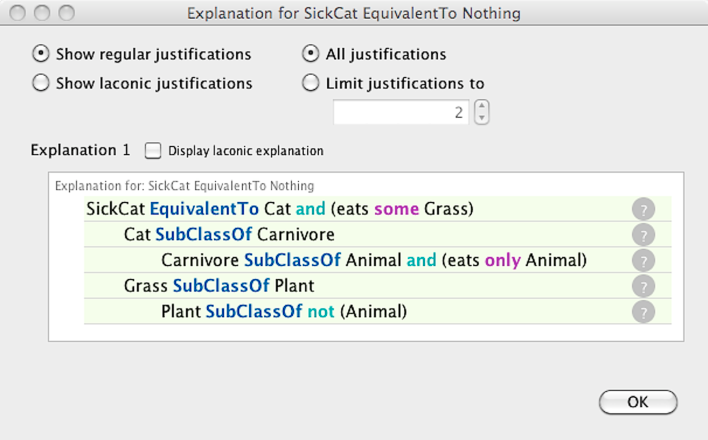
\includegraphics[scale=1]{img/explanation-cat.pdf}
	\caption{A screenshot of the \emph{Explanation} tab in \protege.}
	\label{fig:prot-just-screenshot}
}
\end{figure}

The concept of justifications for description logic ontologies has been widely studied over the past decade, with particular focus on developing efficient algorithms for the computations of all justifications for a given entailment, e.g.\ \cite{schlobach05vd,suntisrivaraporn08aa,du09bn}. There also exist a number of debugging approaches that are closely related to justifications, such as the computation of maximally satisfiable terminologies (MSSs) \cite{meyer06rj,meyer06aa}, which is based on a tableau-like procedure, and the \emph{pinpointing formula} approach proposed by Baader and Pe\~{n}aloza \cite{baader07ur,baader08tp,ji08en,penaloza10ff}.

Rather than directly computing the set of all justifications for an entailment, a pinpointing formula is a compact representation of the set of all justifications for an entailment \cite{baader07ur,baader08tp,penaloza10ff}. A pinpointing formula is a monotone Boolean formula where each propositional variable represents an axiom in the ontology. The set of justifications for an entailment can then be derived from the pinpointing formula as it corresponds to all valuations of the formula. An example of a pinpointing formula is given in \cite{baader07ur}:
\begin{examp}
\begin{alignat*}{2}
 (\alpha_{1})  & \quad\quad & &\dlax{A \subcls \exists r.A}  \\
 (\alpha_{2})  & \quad\quad & &\dlax{A \subcls Y}  \\	
 (\alpha_{2})  & \quad\quad & &\dlax{\exists r.Y \subcls  B}  \\
 (\alpha_{4})  & \quad\quad & &\dlax{Y \subcls B}
\end{alignat*}
\end{examp}
The four axioms labelled with $\alpha_{1}$ to $\alpha_{4}$ entail \dlax{A \subcls B}. We can find two justifications for this entailment: $\J_{1} = \{\alpha_{2}, \alpha_{4} \}$ and $\J_{2} = \{\alpha_{1}, \alpha_{2}, \alpha_{3} \}$. If we treat the axiom labels as propositional variables, the two justifications correspond to the \enquote{true} valuations of the pinpointing formula $\alpha_{2} \wedge ( \alpha_{4} \vee (\alpha_{1} \wedge \alpha_{3} ))$. 

\subsection{Computing justifications}
There exist various approaches to directly computing \emph{one} or \emph{all} justifications for a given entailment, with \enquote{find all} algorithms generally using a \enquote{find one} algorithm as a subroutine. We categorise these algorithms into \emph{glass-box} and \emph{black-box} approaches \cite{kalyanpur05mi}: glass-box techniques generally rely on information provided by a DL reasoner, which requires modification of reasoner internals in order to utilise it for justification computation. By contrast, black-box techniques only use a reasoner as an \emph{oracle} to perform entailment checks.

\subsubsection{Glass-box techniques}

Glass-box justification finding techniques generally rely on the modification of a description logic reasoner to keep track of the axioms required for an entailment to hold, such as those axioms causing a \emph{clash} in a tableaux procedure. More precisely, as the problem of explaining arbitrary entailments, e.g.\ subsumption between classes, can be reduced to a consistency check, this technique can be applied to find justifications for both unsatisfiable classes as well as arbitrary entailments. The tracking strategy applied in glass-box approaches using tableaux reasoners is known as \emph{tracing} \cite{kalyanpur05mi}, which is based on an algorithm first proposed by Baader and Hollunder \cite{baader95aa}. Beyond tableaux-based reasoners, approaches extending the \elplusplus subsumption algorithm \cite{baader07xp} and automata-based approaches \cite{baader08eb,baader10jc} also fall under the label of \enquote{glass box} justification generation. A fair number of approaches to explaining entailments of description logic KBs uses glass-box techniques to present users with reasoner traces in the form of axiom sets, natural language, or some form of visualisation \cite{schlobach03nc,liebig05lf,kwong05aa,meyer06rj}.


\subsubsection{Black-box techniques}

\paragraph{Expand-contract approach}
A simple technique for finding \emph{one} justification for an entailment \ent of an ontology \O is the expand-contract approach \cite{kalyanpur07oq}: in the \emph{expansion phase}, axioms from the given ontology \O are incrementally added to an empty ontology \oprime, performing an entailment check after each addition until it is found that \oprime entails \ent. In order to generate a minimal justification from \oprime, the \emph{contraction phase} then removes superfluous axioms from \oprime, performing an entailment check after each removal. This approach is known as \emph{black-box} technique, as it only requires an out-of-the-box reasoner to perform the entailment checks. Optimisations of this algorithm focus on reducing the number of expensive entailment checks by employing a \emph{divide-and-conquer} \cite{friedrich05rg,shchekotykhin08ay} or a \emph{sliding-window} technique \cite{kalyanpur06nm} in the contraction phase.

\paragraph{Hitting set tree algorithm}
In order to find not only one but \emph{all} justifications for an entailment, Schlobach \cite{schlobach05vd} first proposed the use of Reiter's hitting set tree (HST) algorithm \cite{reiter87pb,greiner89jl} for the computation of \emph{MUPS} and \emph{MIPS}. The algorithm originates from the field of \emph{model based diagnosis}, which describes the process of finding diagnoses for faults in a system comprised of components. A minimal conflict set is a minimal set of such components which causes a system fault, whereby a diagnosis is a minimal \emph{hitting set} across the set of minimal conflict sets. Given a set $C$ of minimal conflict sets, a hitting set for $C$ is a set $H \subseteq \bigcup_{S \in C} S$ such that $H \cap S \not= \emptyset$ for each $S \in C$. Minimal conflict sets and diagnoses correspond to our notion of justifications and minimal repairs, respectively. 

Reiter's algorithm constructs a hitting set tree in order to find all minimal hitting sets over a given set of minimal conflict sets in a diagnosis problem. The nodes in the HST are labelled with minimal conflict sets, and the edges are labelled with components (axioms). For the purpose of finding justifications, the HST algorithm is initialised by computing a single justification using any glass-box or black-box \emph{find one} algorithm, which suffices to generate the tree for \emph{all} justifications, as shown in \cite{kalyanpur07oq}. 

Optimisations, such as \emph{early path termination} and \emph{justification reuse} \cite{kalyanpur07oq} help ensure that the algorithm terminates in practical time. Horridge \cite{horridge11ab} showed that it is possible to compute all justifications for direct atomic subsumptions from over 90\% of the ontologies in a diverse test corpus; for the remaining ontologies, however, the algorithm did not terminate in the given time due to the large size of the constructed HST, or due to a timeout on entailment checks.



\subsubsection{Modularisation} A \emph{module} \module of an ontology \O is a subset of \O which contains all axioms that are relevant for some seed signature $\Sigma \subseteq \sig{\O}$. There exist various types of modules and algorithms for efficient computation of a module for a given seed signature, see, for example \cite{cuenca-grau06ga,cuenca-grau07ci,sattler09jb}. It has been shown that \emph{syntactic locality based modules} are \emph{depleting}, which means that a module generated based on the signature of an entailment contains all justifications for this entailment \cite{cuenca-grau07ci}. Further, for any given seed signature, there exists a \emph{unique} and \emph{minimal} locality based module \cite{cuenca-grau08sj}. 

When used in the justification computation process, a syntactic locality based module \module is computed for the signature of an entailment, and the justification computation deals only with \module rather than the full ontology \O \cite{suntisrivaraporn08aa,du09bn}. Typically, the number of axioms in a module is small compared to the whole ontology \cite{suntisrivaraporn08aa}, which leads to reduced computational load both in the expansion and contract phases, as well as for entailment checks. A study by Suntisrivaporn et al.\ \cite{suntisrivaraporn08yq} using randomly selected entailments from three fairly large and complex OWL ontologies (Galen, NCI, and Gene Ontology) found that the average size of syntactic locality based modules was only between 0.05\% and 1.6\% of the whole ontology. Consequently, the justification computation performance was drastically improved by around two orders of magnitude, making it possible to compute justifications even for entailments on which the algorithm using the full ontology timed out. As the overhead for module computation is neglectable compared to the overall justification computation time, and due to the significant improvements obtained through modularisation, it is now considered a standard optimisation used in justification computation approaches for OWL ontologies.

\subsubsection{Performance}

Generally, glass-box techniques for finding single justifications are considered to be more efficient than black-box techniques, as the justifications are generated almost \enquote{automatically} as a by-product of the classification process. And indeed, in an extensive analysis of various justification computation algorithms, Horridge \cite{horridge11ab} found that using a glass-box \emph{find one} algorithm as subroutine can improve performance by an order of magnitude for some ontologies. However, given the heavy modifications required to integrate tracing with a reasoner, and the fact that currently only the Pellet reasoner supports tracing, we may consider black-box techniques as a more accessible alternative to glass-box approaches.

Regarding the feasibility of computing justifications for OWL ontologies used in practice, Horridge \cite{horridge11ab} found that it is highly likely that we can find \emph{all} justifications for an entailment in reasonable time. His study of 72 ontologies from the NCBO BioPortal showed that for the majority of ontologies in the set (all but 7), all justifications for 99\% of the entailed direct atomic subsumptions could be computed in less than 10 seconds.


\subsection{Justification-based repair}
While justifications offer ontology users a focused view on the subset(s) of the ontology which are relevant to an entailment, they do not provide much guidance as to which steps a user has to take in order to repair the erroneous entailment. Rather, the user is expected to analyse the axioms in the justification and identify a set of axioms \R which can be either removed or modified in order to repair the entailment. A repair over the set of justifications for an entailment \ent is defined as follows \cite{horridge11ab}:
\begin{defn}[Repair]
Given \O \entails \ent, the set of axioms \repair is a \emph{repair for} \ent in \O if $\repair \subset \O$, $\O \setminus \repair \not\entails \ent$, and there is no $\repair' \subset \repair$ such that $\O \setminus \repair' \not\entails \ent$.
\end{defn}

More informally, a repair is a \emph{hitting set} \repair over the set of justifications for \ent in \O, i.e.\ for each justification \J for \ent in \O there is at least one axiom in \J which is contained in \repair. As there are multiple possible repairs for a given set of justifications, we may want to find a \emph{cardinality-minimal} repair, that is, a repair \repair such that there is no repair \repair' with fewer axioms than \repair, as this implies removing or modifying the smallest possible number of axioms. 

The quality of a repair does not only depend on the number of axioms to be removed or modified, but also on the amount of  useful information in the ontology which is \emph{lost} through such modifications. Thus, a suitable repair for an entailment may not be cardinality-minimal, but rather dependent on the \emph{frequency} (\emph{power}, \emph{arity}) and \emph{impact} \cite{kalyanpur06bh} of the axioms in the justifications.

The \emph{impact} \cite{kalyanpur06bh} of an axiom in a justification is the number of entailments (from some clearly defined finite entailment set, such as the set of entailed atomic subsumptions) that are lost when removing the axiom from the ontology. Given a set of justifications for an entailment (or set of entailments), the \emph{frequency} of an axiom is the number of justifications it occurs in, that is, the number of justifications that can be \emph{broken} by removing the axiom. 

\begin{figure}[tb]
\centering{
	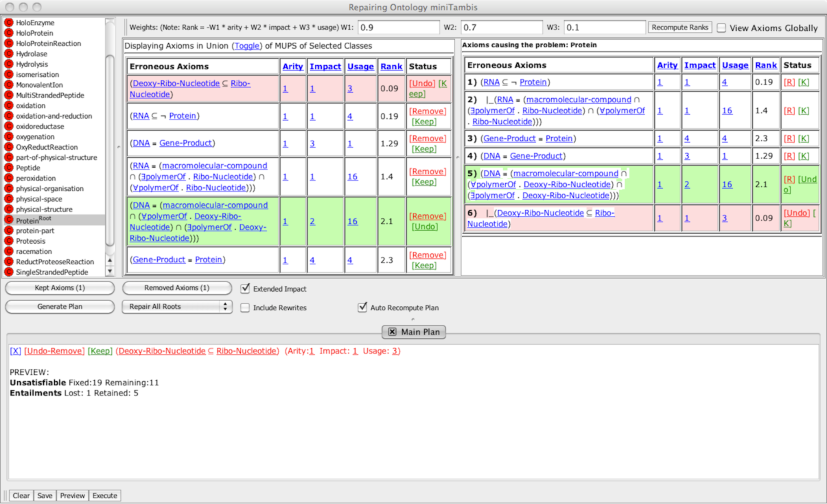
\includegraphics[scale=1]{img/swoop.pdf}
	\caption{A screenshot of the \emph{Repair} tool in \swoop.}
	\label{fig:swoop-screenshot}
}
\end{figure}

Kalyanpur et al.\ \cite{kalyanpur06bh} approached the problem of finding a suitable repair for unsatisfiable classes by introducing a \emph{ranking} on the axioms in justifications. Axioms are ranked according to their frequency, their impact, manually specified test cases by a user (which is an extension to the default impact in order to ensure that specific entailments are preserved), provenance information about the axiom (author, source reliability, time added or modified) and usage of the terms in the axiom signature across the ontology. The repair tool in the \swoop \cite{kalyanpur06sk} editor allows users to specify the weights of the various ranking features, then recommends the preservation or removal of high- or low-ranked axioms, respectively. A screenshot of \swoop's debugging panel is shown in Figure \ref{fig:swoop-screenshot}. While this kind of elaborate debugging support sounds promising, there have not been any in-depth user studies to confirm whether and to which extent ontology developers use the tool and how they benefit from it.

\subsection{Understanding individual justifications}
While the main focus of justification research has been on the performance of justification finding algorithms, in recent years the issue of \emph{understanding} justifications has been receiving increased attention. We know that justifications can significantly reduce user effort by allowing them to focus on a small, \emph{relevant} subset of an ontology; and yet, justifications do not always help all users in understanding the actual \emph{reason} why an entailment holds and in finding a suitable repair.

\subsubsection{Fine-grained justifications}
By definition, a justification is a minimal entailing subset of an ontology; that is, a justification contains axioms as they are \emph{asserted} in the ontology. This means that the axioms in a justification can contain \emph{superfluous} parts, i.e.\ subexpressions on the LHS or RHS of the axiom which do not contribute to the entailment. While such superfluous parts can distract users from the actual cause of an entailment, thus making the justifications more difficult to understand, removing axioms with superfluous parts in the repair process also means a loss of possibly valuable information. 

In order to cope with the issue of superfluity, the notion of \emph{fine-grained} justification was first introduced by Kalyanpur et al.\ \cite{kalyanpur06fj}. This approach was based on the idea of re-writing justification axioms in a normalized form, then splitting the axioms across intersections and only preserving those axioms which are required for the entailment in question to hold. The strategy was implemented in the Swoop editor, using strike-out and colour highlighting to indicate superfluous expressions in axioms---a simple, yet visually effective technique. Lam et al.\ \cite{lam06tk} directly integrated the idea of fine-grained justifications into a repair tool, computing the impact of each axiom rewriting based on the modification of its \emph{subexpressions}.

Based on these first attempts, Horridge et al.\ \cite{horridge08yi} firstly proposed a definition for \emph{laconic} justifications: a laconic justification is a justification which does not contain any superfluous parts, with every subexpression being as \emph{weak} as possible \cite{horridge08yi}. This implies that every subexpression in a laconic justification is relevant to the entailment. The authors \cite{horridge08yi} also describe a method to compute the \emph{preferred} laconic versions of a justification which results in a unique correspondence between a justification and its laconic variants. In short, the process
\begin{compactitem}
\item removes any subexpressions from axioms which are not relevant for the entailment to hold.
\item derives a single subsumption axiom from an equivalence where possible.
\item substitutes class names with the \thing where possible.
\item weakens number restrictions to the smallest number possible.
\end{compactitem}

The following example illustrates several aspects of non-laconicity in a justification:
\begin{examp}
\begin{align*}
\J &=  \{ A \sqsubseteq B ~\conj \leq2 r.C, \exists r.C \sqsubseteq D\} \models A \sqsubseteq D
\end{align*}
\end{examp}
First, we can reduce the intersection in the first axiom to the single expression $\leq2 r.C$ without affecting the entailment. Second, this expression can then be weakened to $\leq1 r.C$. Third, the class name $C$ in both axioms can be substituted with \thing. This results in the laconic justification $\{ A \sqsubseteq \leq1 r.\top, \exists r.\top \sqsubseteq D\}$. 

A survey \cite{horridge11ab} of 72 of OWL ontologies from the NCBO BioPortal\footnote{\url{http://bioportal.bioontology.org/}} revealed that non-laconic justifications are prevalent across OWL ontologies; indeed, the majority of the surveyed ontologies (69 out of 72) contained at least some non-laconic justification for an atomic subsumption, with 29 ontologies containing over 50\% non-laconic justifications. 

\subsubsection{Masking}
Justification \emph{masking} \cite{horridge08yi,horridge10bg} occurs when the actual number of \emph{reasons} why an entailment holds differs from the number of justifications that can be found for the entailment. There exist different types of masking, which are mainly caused by axioms containing superfluous expressions, i.e.\ being non-laconic. The examples given in \cite{horridge10bg} focus on unsatisfiable classes; it can easily be shown, however, that masking also occurs for arbitrary entailments.

\emph{Internal masking} describes a situation where the justification contains more than one reason why an entailment holds, which means that there exist multiple laconic versions of the justification.
\begin{examp}\begin{align*}
\J &=  \{ A \sqsubseteq B \conj C, B \disj C \sqsubseteq D\} \models A \subcls D
\end{align*}\label{ex:internalmasking}\end{examp}
Example \ref{ex:internalmasking} shows a justification \J for \dlax{A \subcls D} which contains two reasons for the entailment. The laconic versions of \J are:
\begin{align*}\J_{1} &=  \{ A \sqsubseteq B, B \sqsubseteq D\}\\
\J_{2} &=  \{ A \sqsubseteq C, C \sqsubseteq D\}\end{align*}

\emph{External masking} involves other axioms from the ontology which do \emph{not} occur in any justifications for an entailment. 
\begin{examp}\begin{align*}
\O &=  \{ A \sqsubseteq C \conj  D, C  \sqsubseteq D\} \entails A \sqsubseteq D
\end{align*}\label{ex:externalmasking}\end{examp}
In the ontology shown in Example \ref{ex:externalmasking} there exists only one justification for the entailment \dlax{A \subcls D}, namely the first axiom \dlax{A \subcls B \conj C}. It is clear to see, however, that the two axioms in \O combined result in another reason for the entailment---but the justification comprising both axioms would violate the minimality condition for justifications.

\emph{Cross masking} is similar to external masking with the difference that the axioms involved are from other \emph{justifications} for the same entailment rather than non-justification axioms.
\begin{examp}\begin{align*}
\J_{1} &=  \{ A \sqsubseteq C \conj D \}\\ 
\J_{2} &=  \{ A \disj C \sqsubseteq D\}
\end{align*}\label{ex:crossmasking}\end{examp}%
In addition to the two justifications $\J_{1}$ and $\J_{2}$ for the entailment $A \sqsubseteq D$, there exists a third reason why the entailment holds, which comprises parts of both justifications: $ \{ A \subcls C, C \subcls D\} \entails A \subcls D$. Again, this third reason,  comprising both axioms, cannot be a justification, as it is non-minimal.

\emph{Shared cores masking} occurs when two \emph{different} justifications have the same reason why an entailment holds, i.e.\ they only differ in their superfluous parts. This implies that the actual number of explanations for an entailment is \emph{lower} than it appears.
\begin{examp}\begin{align*}
\J_{1} &=  \{ A \sqsubseteq D\}\\ 
\J_{2} &=  \{ A \sqsubseteq D \conj \exists r.C\}
\end{align*}\end{examp}
An ontology which contains the two axioms in $\J_{1}$ and $\J_{2}$ has two distinct justifications for the entailment $A \sqsubseteq B$. However, the actual reasons why the entailment holds are identical, as the laconic version of $J_{2}$ is identical to $J_{1}$. 

Masking may cause problems for users attempting to understand or repair an entailment. When repairing a justification where internal, external, or cross masking occurs, a user might only notice and modify one of the reasons, expecting the entailment to no longer hold after the modification. That modification, however, may lead to \emph{another} justification for the entailment---an effect which may be rather surprising. Worse even, the justification may interact with several other axioms to create multiple justifications, a situation which has been found to occur in the NCI thesaurus \cite{horridge11ab}. Furthermore, when analysing justifications for the purpose of gathering ontology metrics, justification masking may lead to over- or under-counting the number of \emph{actual} justifications in an ontology.

It is clear to see that ontology debugging tools need to support users in cases where masking occurs through non-laconicity. Dealing with superfluity in an explanation tool, however, makes it necessary to balance two opposing requirements: first, we want the user to be presented with the most concise explanation as to why an entailment holds, and avoid cluttering and distraction caused by superfluous parts. Second, in order to facilitate understanding and repair, the explanations should directly relate to the asserted axioms in the ontology. To date, there have been no successful approaches to OWL ontology debugging that meet both requirements.
 
 
\subsubsection{Justification-based proofs}
\label{sec:justproofs}
In addition to superfluity, there exist other reasons why a justification can be difficult to understand. Justifications may contain structural patterns and constructors whose implications are unfamiliar or non-obvious to the user. A popular example from the \emph{Movie} ontology illustrates how even a very small justification can be hard to impossible to understand for OWL experts \cite{horridge09zp,horridge10gs}: 
\begin{examp}\begin{align*}
		\J = \{ &\ax{Person \sqsubseteq \neg Movie},\\
		&\ax{RRated \sqsubseteq CatMovie},\\
		&\ax{CatMovie \sqsubseteq Movie},\\
    	&\ax{RRated \eqcls \exists hasScript.ThrillerScript \disj \forall hasViolenceLevel.High},\\
    	&\ax{domain(hasViolenceLevel, Movie)} \} \entails \ax{Person \subcls \nothing}
	\end{align*}\label{ex:movie}\end{examp}
Example \ref{ex:movie} shows a justification for the unsatisfiability of the class \cn{Person} in the \emph{Movie} ontology. Axioms 2 to 5 in the justification entail that \ax{Movie \eqcls \thing}, which implies that \ax{Person \subcls Movie}, which, in turn, contradicts the first axiom that states the disjointness of the classes \cn{Person} and \cn{Movie}. When presented with this justification, subjects tend to give up or question the correctness of the justification \cite{horridge10gs}.

\emph{Justification-based proofs} seek to address the problem of understanding such justifications by providing users with a more detailed explanation which includes not only the justification axioms, but also intermediate entailments such as \ax{Movie \eqcls \thing} in the previous example. Such intermediate entailments, arising from subsets of a justification \J are known as \emph{lemmas}.

In a similar approach to justification-based proofs, Nguyen et al.\ \cite{nguyen12aa} generate natural language proofs based on justifications by identifying frequent sub-patterns, or \emph{rules}, in justifications which lead to such intermediate entailments, then translating the proof trees into natural language. They extracted patterns, restricted to laconic axioms and a maximum size of 4 axioms, from 500 OWL ontologies and identified the 57 most frequent patterns, which are then used as the basis for natural language proofs.


\subsubsection{Cognitive complexity}

To date, there have only been few attempts at investigating the understandability of justifications for OWL users. While there exists a number of user studies to evaluate OWL debugging tools \cite{kalyanpur05mi,lam07aa}, they focus on measuring the time and success rates of the debugging tools and do not offer any further insights into how users interact with the explanations. The first major study on the cognitive complexity of justifications was carried out by Horridge et al.\ \cite{horridge11gj} for the purpose of evaluating a complexity model for justifications which was constructed based on an initial exploratory study \cite{horridge11si}. The study involved 14 students from an MSc class who were presented with a set of items consisting of a set of axioms and an entailment, and were asked to answer whether the entailment followed logically from the axiom set or not. It was found that the complexity predicted by the model coincided partially with the error rate in this task, with some anomalies in the error rates caused by a) superfluity in a justification which the model did not account for, and 2) by a \enquote{flaw} in the experiment protocol which meant test subjects could answer the question correctly, but (presumably) for the wrong reason.

Building on their work on justification-based proofs, Nguyen et al.\ \cite{nguyen12ab}  present an investigation of the difficulty users have with understanding various sub-patterns that occur in OWL justifications. The authors conducted a study on a \enquote{mechanical turk} like web platform where test subjects were presented with natural language reasoning problem which was directly based on one of the 51 (out of 57 identified) justification sub-patterns. Each problem was answered by around 50 people, with correct answers ranging from 100\% for the easiest rule to only 2\% for the most difficult one. While natural language based explanation is potentially highly effective for OWL novices, the resulting proofs are often very large and might be difficult to navigate and understand themselves. 


\subsection{Understanding multiple justifications}

In many ontologies used in practice, we find that there exist multiple justifications for a single entailment. While the possible number of justifications per entailment is exponential in the number of axioms in the ontology \cite{baader07xp}, the average number of justifications found in OWL ontologies is comparatively small \cite{bail11jm}. However, even for justification counts way below the exponential threshold, we are often faced with several dozen to several hundred justifications for a single entailment. When attempting to repair an ontology, such numbers are clearly not suitable for manual repair by a user; and even with a justification-based repair tool which displays all justifications as a list, there is hardly any chance of producing a minimal repair.

Ji et al.\ \cite{ji08en} propose a strategy for reducing the number of justifications a user is confronted with by only computing justifications that are the most \emph{relevant} for an entailment. The approach, which was implemented as part of a plugin to the NeOn Toolkit\footnote{\url{http://www.neon-toolkit.org/}} ontology editor, introduces a selection function based on the amount of signature a justification shares with the entailment. While this relevance-based approach may be helpful when users require only a few justifications for \emph{understanding} an entailment, it does not solve the problem of helping a user repair \emph{all} justifications to break an unwanted entailment.

\subsubsection{Root and derived justifications}
\label{sec:rootderived}

\emph{Root and derived} justifications provide an additional form of explanation support which aims to assist users in the simultaneous repair of multiple entailments. The idea of unsatisfiable classes depending on the unsatisfiability of another class was originally mentioned in \cite{schlobach05tf} and explicitly introduced as root and derived unsatisfiable classes \cite{kalyanpur05mi}. While the initial focus was on entailed unsatisfiable classes, the concept can be easily extended to arbitrary entailments, as shown in \cite{meyer10vd}: given a set of entailments \entset and their justifications \justs, a \emph{derived} justification $\J_{D} \models \eta_{D}$ is a justification which is a superset of some other justification $\J, \eta$. Repairing \J first (e.g.\ by removing or modifying an axiom) will also repair $\J_{D}$. Note that there may be additional reasons for $\eta_{D}$ to hold, which are not covered by this process. A \emph{root} justification is a justification $\J_{R}$ in \justs which is not a superset of any other justification in \justs.

\begin{defn}[Root and derived justifications]
Let \entset be a set of entailments of interest, and \just a justification for an entailment \ent in \entset. \just is called a \emph{root} justification if there exists no justification $\just'$ for an entailment in \entset such that $\just' \subset \just$, else, \just is called a \emph{derived} justification.
\end{defn}

Kalyanpur et al.\ \cite{kalyanpur05mi} carried out the first user study for explanation support in OWL, evaluating the debugging facilities of the ontology editor Swoop. The 12 study subjects were randomly divided into four groups and were given the task to repair unsatisfiable classes in three OWL ontologies using one of three types of debugging tools (clash information from the reasoner and sets of support, root and derived unsatisfiable classes, both), with the fourth group receiving no debugging support at all. Perhaps unsurprisingly, the study found that the group using both the clash information, sets of support (i.e.\ justifications) and root and derived information performed best (i.e.\ fastest) in this task.



\section{Alternative approaches to debugging}
Besides justifications (and approaches closely related to the concept of justifications), there exists a number of alternative approaches to ontology debugging. While these may not be as prevalent as justifications in OWL ontology tools, they represent some relevant solutions to the problem of understanding and debugging formal ontologies, such as proofs, natural language techniques, and semi-automated debugging strategies. Under this label, we also gather other approaches to visualising and understanding ontologies, which, while not explicitly tailored towards debugging, may be helpful tools for understanding and repairing entailments.

\subsection{Proofs}

Formal proofs are considered to be the most prevalent alternative form of explanation for logic-based knowledge bases. One of the first approaches to explaining entailments in the CLASSIC system using proof-like structures was presented by McGuinness and Borgida \cite{mcguinness95jb}. The system omits \enquote{obvious} intermediate steps and provides further filtering strategies in order to generate short and simple explanations. Borgida et al.\ \cite{borgida99cn} first introduced a proof-based explanation system for knowledge bases in the Description Logic \dl{ALC}. The system generates sequent calculus \cite{83aa} style proofs using an extension of a tableaux reasoning algorithm, which are then enriched to create natural language explanations. Aiming to \enquote{provide the simplest explanation possible}, the authors also introduce a \emph{relevance} function which simplifies the proofs by omitting \enquote{irrelevant} parts. The consensus of these proof-based approaches seems to be that good proofs ought to be \enquote{as simple and short as possible}, yet, there have been no formal investigations into how ontology developers interact with such proof-based explanations. 

While proof presentation in other logics has been well studied (e.g.\ \cite{felty1988aa}), surprisingly few authors are concerned with the cognitive aspects of proof understanding. There exist formal definitions of \emph{obvious proof steps} \cite{davis81sz, rudnicki87om}, however, these are merely formulated with the goal of creating \emph{short} proofs and do not investigate other sources of complexity for human readers. By comparison, Lingenfelder \cite{lingenfelder89rm} also considers the skill level of the proof reader to be crucial in order to determine what can be considered \enquote{trivial} in a proof, and emphasises the need for a \emph{user model} in order to provide suitable proofs. 

\subsection{Ontology revision}

Ontology revision as described by Nikitina et al.\ \cite{nikitina12aa} follows a semi-automated approach to ontology repair, with a focus on factually incorrect statements rather than logical errors. In the ontology revision process, a domain experts inspects the set of ontology axioms, then decides whether the axiom is correct (should be accepted) or incorrect (axiom is rejected). Each decision thereby has consequences for other axioms, as they can be either automatically accepted (if they follow logically from the accepted axioms) or rejected (if they violate the already accepted axioms). 

The ontology revision system determines the impact a decision has on the remainder of the axioms (using a ranking function), and presents high impact items first in order to minimize the number of decisions a user has to make. Conceptually, this approach is straightforward and easily understandable for a user, as the cognitive effort is reduced to a simple yes/no decision, and the tool attempts to minimize the number of decisions that need to be made. In order to debug unwanted entailments, e.g.\ unsatisfiable classes, the set of unwanted consequences can be initialised with those erroneous axioms. The accept/decline decisions are then made in order to remove those axioms which lead to the unwanted entailments. 

\subsection{Direct computation of diagnoses}

The direct diagnoses computation approach \cite{friedrich05rg,du08eo,shchekotykhin12aa,rodler12aa} is directly related to justifications, but rather than computing the set of justifications for an entailments which is then repaired by repairing or modifying a minimal hitting set of those justifications, the diagnoses (i.e.\ minimal hitting sets) are computed directly. The direct computation of diagnoses using the hitting set tree algorithm was first proposed by Friedrich and Shchekotykhin \cite{friedrich05rg}. The authors argue that debugging large numbers of conflicts and potentially diagnoses by computing justifications poses a computational challenge, while direct computation of diagnoses provides a more efficient solution. 

Both the ontology revision approach by Nikitina et al.\ and the direct computation of diagnoses show some advantages over computing justifications in terms of computational performance. However, the semi-automated repair presented in \cite{nikitina12aa} means that the user has no direct control over which axioms to remove or modify in order to repair the unwanted entailments, while the direct computation of diagnoses aims exclusively at finding a minimal repair, regardless of the factual correctness or incorrectness of the axioms involved in the diagnoses. Furthermore, neither of the approaches supports \emph{understanding} why those entailments hold, as the users are not presented with the actual \emph{reasons}, but only see a sequence of axioms or a set of diagnoses, respectively. While both approaches aim to reduce the total number of steps taken in the debugging process, they might still require a user to go through a long and tedious revision process when repairing a large number of errors.

\subsection{OntoClean}

OntoClean \cite{guarino02aa,guarino04aa} provides a framework for making modelling decisions in the ontology development process, with a strong focus on correct subumption relationships. This is motivated by a misuse of subsumptions to express other relations than is-a relationships, for example part/whole relationships. OntoClean helps users to validate taxonomies by identifying \emph{metaproperties} of each class, such as \emph{rigidity}, \emph{identity}, \emph{unity}, and \emph{dependency}. The framework then specifies constraints on subsumptions between classes with different properties, such as if a class \dlcn{A} is anti-rigid, i.e.\ an instance of \dlcn{A} can \emph{cease} to be a member of the class, then every subclass of \dlcn{A} must also be anti-rigid. By applying OntoClean guidelines when building taxonomies, ontology developers can prevent subsumption relationships which may later lead to modelling inconsistencies.

\subsection{Ontology comprehension}

Ontology users often require support in understanding an ontology, or parts of it, for example, when integrating an existing ontology into a project, which requires the ontology developer to familiarise themselves with the structure of the adopted ontology. While not specifically aimed at ontology debugging, such comprehension and visualisation tools can  help users to get a better grasp of the relationships between entities in an ontology, which may provide support in the debugging process.

Ontology visualisation tools, such as the OWLViz plugin\footnote{\url{http://www.co-ode.org/downloads/owlviz/}} in \protege, the CropCircles tool \cite{wang06wr} and the, admittedly rather exotic, music score notation of Barzdins and Barinskis \cite{barinskis07uz}, offer ontology users support when exploring an ontology in order to gain an overview of the relationships between its classes.

Visualisation techniques can also be used for the purpose of \emph{model exploration} \cite{bauer09ru}, which can user support in understanding \emph{non-entailment}. Users may want to understand, for instance, why a class is not entailed to be subclass of some other---a fact that cannot be explained by justifications, as it is not possible to point out a particular subset of the ontology that does \emph{not} entail something. The idea underlying model exploration is that seeing (subsets of) the models of an ontology helps users understand the relations between its classes, which, in turn, may support them in understanding why an entailment holds or does \emph{not} hold in the ontology.


\section{Summary and conclusions}
In this chapter, we have laid out the foundations for the work presented in this thesis. We introduced the basic concepts of description logic knowledge bases, such as their syntax, semantics, and standard reasoning services, and introduced the Web Ontology Language OWL. We discussed the scope of logical and non-logical errors which can occur in OWL ontologies and introduced justifications as the currently dominant form of debugging support for entailments of OWL ontologies. This was followed by a closer look at the strategies for computing justifications, as well as some of the applications of justifications for repairing errors in OWL ontologies. Finally, we gave an overview over debugging strategies for description logic knowledge bases which are not directly related to justifications or only make indirect use of them, finding that the majority of approaches do not consider cognitive aspects of how users interact with explanation.

While multiple justifications for entailments of OWL ontologies have been acknowledged as a phenomenon to be found in OWL ontologies, the main focus of research thus far has been the efficiency of computing multiple justifications. In contrast, the issue of how users can find a suitable repair once those justifications have been computed has been largely neglected. There exist some approaches to making individual justifications easier to understand, such as laconic justifications and justification-based proofs, but the specific problem of debugging and repair in the presence of multiple justifications has not been addressed in prior research, except for some work looking at root and derived unsatisfiable classes. Root and derived unsatisfiable classes provide a first level of additional support for a particular relationship between multiple justifications for multiple entailments; yet, there have been no investigations into whether root/derived relationships are indeed a common feature of OWL justifications, what steps can be taken when this feature is not present, and how users can cope with multiple justifications for \emph{single} entailments. Besides, while root and derived unsatisfiable classes indicate that there exist structural relationships between justifications, there have not been any investigations into other such relationships and whether they can be exploited for debugging.

In summary, there does not seem to be a good understanding of how prevalent multiple justifications are in ontologies used in practice, neither are there sophisticated enough coping strategies to help ontology engineers deal with multiple justifications efficiently. These insights motivate the research presented in this thesis, as there is an obvious need for further investigation of the occurrence of multiple justifications, the relations between them, and techniques for reducing both mechanical (the number of steps taken to achieve a goal) as well as mental (the cognitive complexity of the information presented to a user) user effort in the presence of multiple justifications.
\chapter{Defining finite entailment sets}
\label{chap:entailments}
The justificatory structure of an OWL ontology \O describes the relationships between the justifications for \emph{some} set of entailments of \O. However, if we want to compute the set of justifications for \enquote{the entailments} of an ontology, we immediately encounter a problem: recall that the set of entailments of an ontology \O is the set of all axioms \axiom such that \O \entails \axiom---a set which is infinite for OWL ontologies, and in most cases it does not seem practical to compute and analyse justifications (other than the empty ontology over a non-empty signature) for an infinite set of entailments. 

Thus, we need to restrict the set of entailments we analyse to some \emph{finite} subset of the deductive closure of \O. Classification of an ontology, that is, computing all entailed subsumptions and equivalences containing only named classes, is a standard reasoning task, and the resulting class hierarchy (in the form of either the atomic subsumption axioms or both subsumption and equivalence axioms) of the ontology is a commonly used entailment set in OWL applications.

However, even if we restrict our attention to the class hierarchy of an ontology, we find that there is no standard way of \emph{representing} this set of axioms. Worse even, misleading nomenclature in ontology tools, such as the \protege editor and the OWL API, as well as anecdotal evidence show that there exist common misconceptions about the entailments: it is often assumed that only non-trivial information is contained in the set of entailments, and tautologies such as \dlax{A \subcls A} are not \enquote{real} entailments. On the other hand, however, some OWL tools \emph{do} include tautologies of the type \dlax{A \subcls \thing} for certain named classes. And finally, the term \enquote{entailments} is frequently used to refer to information which is only \emph{inferred} but not asserted in the ontology, leading to asserted axioms not being considered entailments.

This means that, despite having a well-defined finite set of entailments at hand (the set of all axioms $\alpha$ of type \dlax{A \subcls B} and, if required, \dlax{A \eqcls B} for $A, B \in \sig{\O}$ such that $\O \models \alpha$), we still obtain different numbers of entailments for the same ontology depending on the representation chosen by the application we are dealing with. And while it may not be necessary to define a single canonical representation of the class hierarchy---after all, axioms such as \dlax{A \subcls \thing} \emph{can} be useful for some applications while they might be superfluous in others---we need to at least make obvious the different design decisions to be made when choosing a representation for this entailment set.

In what follows, we will discuss various design decisions for representing finite entailment sets  of consistent OWL ontologies, which takes into consideration relationships such as direct and indirect subsumptions, tautologies, dealing with unsatisfiable and universal classes, and ontology imports, while paying attention to the issue of \emph{counting} entailments. The design decisions presented here largely focus on the class hierarchy of an ontology, but are also applicable to arbitrary entailments, and we will also discuss how we can define finite entailment sets \emph{beyond} the simple class hierarchy of an ontology. Finally, we introduce a shorthand notation which allows us to conveniently refer to a specific representation of an entailment set, and outline some examples of how entailment sets are used in OWL applications. 

While this chapter informs the experiments on justifications presented in the remainder of this thesis, it may also be regarded as a self-standing discussion with relevance to applications such as ontology analysis, the OWL API, and ontology editing tools.


\section{Design decisions for finite entailment sets}

In this section, we will describe a number of design decisions to make when choosing a representation for a finite entailment set of an OWL ontology. In other words, given a finite set of entailments, such as the axioms representing the class hierarchy, we suggest a set of filtering steps which result in an axiom set that is logically equivalent, but may differ in the number of axioms it contains.

To clarify the distinction between a finite entailment set and its representation, consider a simple example: given an ontology \O = $\{A \subcls B, B \subcls C\}$, we are interested in all entailed atomic subsumptions of type \dlax{X \subcls Y} where $X \not= Y$, $X \not= \nothing$, and $Y \not= \thing$. This gives us the finite entailment set \entset = $\{A \subcls B, B \subcls C, A \subcls C\}$. However, we may also choose to \emph{represent} \entset by an equivalent, more compact set of axioms \entset' = $\{A \subcls B, B \subcls C\}$, which is logically equivalent to \entset, but contains fewer axioms. 

Only the choice of entailment types has an effect on the actual \emph{size} of a finite entailment set: given two ontologies \O and \oprime such that $\O \subset \oprime$, we expect the number of axioms in a finite entailment set of the \emph{larger} ontology \oprime to be the same or more than that of \O. That is, our notion of finite entailment sets must be \emph{stable} under the extension of an ontology \O; an essential criterion when using entailment counts for the comparison of two ontologies. 

However, as we will see in the following sections, some design decisions for \emph{representations} of entailment sets appear to violate the stability of the entailment set relation by leading to \emph{smaller} (representations of) entailment sets when \emph{adding} axioms to an ontology. Where applicable, we will point out the impact of a decision on the stability of entailment counts.


\subsection{Tautologies}
A tautology is an axiom such as \dlax{A \subcls A}, \dlax{A \subcls \thing}, and \dlax{\nothing \subcls A} for a named class \dlcn{A \in \sig{\O}} which is vacuously entailed by \O. Tautologies do not contain any relevant information and are therefore frequently omitted from the axiom set representing the class hierarchy of an ontology.

However, in some OWL tools, such as the OWL API and \protege, named classes that do not have a direct named subsumer are generally \emph{included} in entailment sets as subclasses of \thing, in order to ensure that all named classes in the ontology are present in the entailment set in some way. Note that this strategy means that \emph{only} classes which do not have a named subsumer occur in axioms of the type \dlax{A \subcls \thing}. This can be problematic if we use the entailment count to compare the logical strength of two ontologies: take, for instance, two ontologies over the signature $\{A, B, C\}$ where \O = $\emptyset$ and $\oprime = \{A \subcls B\}$. If we include axioms of the above type in the entailment set, we get the two entailment sets 
\begin{align*}
\varepsilon_{\O} =& \{ \dlax{A \subcls \thing}, \dlax{B \subcls \thing}, \dlax{C \subcls \thing}\}\\
\varepsilon_{\oprime} =& \{\dlax{A \subcls B}, \dlax{B \subcls \thing}, \dlax{C \subcls \thing}\}.
\end{align*}
Both entailment sets have the same number of entailments; however, $\varepsilon_{\oprime}$ arguably contains at least \emph{some} non-trivial information (namely the subsumption \dlax{A \subcls B}). While this decision does not affect the monotonicity of the entailment count, it shows that, if we include tautologies in an entailment set, the size of the set may not reflect the amount of relevant information it contains.

Since there is no obvious benefit to including most tautologies in a finite entailment set, we will generally consider finite entailment sets to be free of tautologies in the remainder of this chapter. If required, we may only include axioms of the type \dlax{A \subcls \thing} for a named class \dlcn{A} which does not have any other named subsumer. 


\subsection{Asserted and inferred axioms}

Every axiom that is asserted in an ontology \O is trivially entailed by the ontology and therefore part of the set of entailments of \O. However, the main idea behind logic-based ontologies is the application of automated reasoning to make \emph{implicit} knowledge visible; thus, the set of \emph{inferred}, but not asserted, axioms may be of much higher relevance to a user. In particular when counting entailments of an ontology, including asserted axioms in the count may not add any useful information if the number of asserted axioms of the selected type is already known. Most OWL tools (e.g.\ \protege and the OWL API) take this into account when representing the class hierarchy of an ontology and return only entailments which are inferred, but not asserted.

While excluding asserted axioms from an entailment set is a reasonable choice in user-focused applications, this may lead to a loss of information in analytical applications, such as justification analysis. An entailment that is asserted in an ontology may also hold for other, more complex reasons, i.e.\ it can have justifications other than the asserted axiom itself. This may be purely accidental and a side-effect of other axioms in the ontology, or intentional as a result of ontology developers \enquote{adding} inferred entailments into the ontology. Making entailments explicit has two advantages: first, it may improve reasoner performance when classifying the ontology, as the reasoner will have to perform fewer subsumption checks, and second, the information will be visible even when there is no reasoner available, for example in a web-based ontology browser---and even if these are not real benefits, users may \emph{believe} that they are, which encourages them to take these steps. 

When counting entailments, we need to be aware of the effects of excluding asserted entailments from the entailment set. Assume an ontology \O with $n$ asserted atomic subsumptions and $k \geq 1$ inferred (but not asserted) atomic subsumptions. If we only count entailments which are inferred but not asserted, the entailment count for \O will be $k$. Now, if we add all $k$ inferred atomic subsumption axioms to \O, we obtain \oprime such that $\O \subset \oprime$. Then the entailment set of \oprime will contain no (inferred but not asserted) axioms, that is, $\varepsilon_{\oprime} \subset \varepsilon_{\O}$ despite $\O \subset \oprime$. This is obviously counter-intuitive, as we generally expect the number of entailments to grow monotonically as we add axioms to an ontology. 

A more concrete example shows how the distinction between inferred and asserted entailment makes the entailment count dependent on the syntactical variations of equivalent axioms: take $\O = \{\dlax{A \subcls B \conj C}\}$ and $\oprime = \{\dlax{A \subcls B}, \dlax{A \subcls C}\}$. \O has two entailed atomic subsumptions (\dlax{A \subcls B}, \dlax{A \subcls C}) which are inferred and not asserted, whereas \oprime, despite having the same entailed atomic subsumptions, has no entailments according to our specification.

Of course, in both examples the \enquote{missing} entailments are only a deception, as the two ontologies are logically equivalent, which means they do not actually differ in terms of their information content; however, if we use that the number of inferred (and not asserted) entailments as an ontology metric to compare the two ontologies, we can easily see how this situation can quickly lead to counting errors.


\subsection{Transitivity}

We generally treat the class hierarchy of an ontology as a directed graph, with nodes representing sets of equivalent classes, and edges representing subsumption relationships. A \emph{direct} subsumption between a class \dlcn{A} and a class \dlcn{B} is represented by an edge between the nodes labelled with \dlcn{A} and \dlcn{B}, respectively; this corresponds to a path of size one. An \emph{indirect} subsumption is a path between two nodes of size greater than one. The class graph can be either based on the \emph{asserted} ontology, i.e.\ the class graph is constructed based on the axioms in the ontology, without the use of a reasoner, or the \emph{inferred} ontology, which means that the class graph is built according to the subsumptions and equivalences returned by a reasoner. That is, a directed edge between the nodes labelled \dlcn{A} and \dlcn{B} is added to the class graph of \O if \dlax{A \subcls B} is asserted in (inferred by) \O, and a class name \dlcn{C} is added to the label of a node labelled $\{D\}$ if \dlax{C \eqcls D} is asserted in (inferred by) \O. Note that in \protege, the class hierarchy display is generated using a very simple \emph{structural} reasoner which, in addition to implementing transitivity of the subsumption relationship, simply splits conjunctions on the RHS of subsumption axioms and in equivalent classes axioms.

The set of all entailed atomic subsumptions, direct and indirect, then corresponds to the transitive \emph{closure} of the inferred class graph, while the transitive \emph{reduct} \cite{aho72pz} represents the set of entailed \emph{direct} subsumptions. The transitive reduct of a directed acyclic graph $G$ is a graph $G'$ such that $G'$ has a directed path between two nodes $u,v$ whenever there is a path ($u, v$) in $G$, and there is no graph with fewer edges than $G'$ which fulfils that condition. The abstract concept of a transitive reduct can be represented as the Hasse diagram\footnote{See, for example, \cite{joslyn06aa} for an example of diagrammatic representations of an OWL ontology.} of an ontology's class graph.

There are several scenarios in which we may want to include or exclude indirect subsumptions in a representation of the class hierarchy. When presenting a set of entailed axioms to a user, we may  assume that the user understands the principle of transitivity and only requires a small entailment set with \emph{relevant} information; in such a case, it seems reasonable to choose a compact representation of the entailment set by excluding indirect subsumptions. On the other hand, if a user wants to be presented with \emph{all} the information entailed by an ontology, it might be preferable to include indirect subsumptions. For the purpose of computing and analysing justifications of an ontology, for example, we may want to include indirect subsumptions in the entailment set, as they may have relevant justifications which would otherwise be neglected.

With regards to counting the number of entailments of an ontology, care needs to be taken when dealing with the transitive reduct of the inferred class graph. Example \ref{ex:transreductontology} shows how \emph{removing} axioms from an ontology results in an \emph{increase} in the number of entailments.
\begin{examp}\begin{align*}
		\O = \{&\dlax{X_{1}  \subcls A}, \dlax{X_{2}  \subcls A}, \dlax{X_{3}  \subcls A}\\
		&\ax{X_{1}  \subcls B}, \dlax{X_{2}  \subcls B}, \dlax{X_{3}  \subcls B}, \dlax{A \subcls B} \}\end{align*}\label{ex:transreductontology}\end{examp}
Given the above ontology, the number of entailed direct atomic subsumptions, based on the transitive reduct of the inferred class graph (shown in Figure \ref{fig:inf-classgraph-before}), is 4, as the indirect subsumptions between \dlcn{X_{i}} and \dlcn{B} are excluded from the set: $\entset = \{\dlax{X_{1}  \subcls A},  \dlax{X_{2}  \subcls A}, \dlax{X_{3}  \subcls A}, \dlax{A  \subcls B} \!\:\}$. Removing the axiom \dlcn{A \subcls B} from the ontology creates the class graph for the now modified ontology \oprime shown in Figure \ref{fig:inf-classgraph-after}; as we can see, the transitive reduct of the graph has \emph{more} edges than the graph for \O. Accordingly, the set of entailments based on the transitive reduct now contains 6 entailed axioms: $\varepsilon_{\oprime} = \{\dlax{X_{1}  \subcls A},  \dlax{X_{2}  \subcls A}, \dlax{X_{3}  \subcls A}, \dlax{X_{1}  \subcls B},  \dlax{X_{2}  \subcls B}, \dlax{X_{3}  \subcls B}\!\:\}$. Thus, the removal of an axiom has led to a seemingly \emph{larger} entailment set in this particular representation.

\begin{figure}
\centering
		\begin{subfigure}{0.5\textwidth}
                \centering
                \begin{tikzpicture}
\tikzstyle{every node}=[draw,shape=circle];

  \node (b) at (1.5,3) {$B $};
  \node (a) at (1.5,1.5) {$A$};
    
  \node (x1) at (0,0) {$X_{1}$};
  \node (x2) at (1.5,0) {$X_{2}$};
  \node (x3) at (3,0) {$X_{3}$};
\foreach \from/\to in {a/b, x1/a, x2/a, x3/a}
\draw [->,thick] (\from) -- (\to);
    
    
\draw[->,line width=0.5pt, color=white]  (x2.south) to [out=-90,in=-90]  ([xshift={-10}]x1.west) to [out=90,in=-180] (b.west);

\end{tikzpicture}


                \caption{Transitive reduct of \O.}
        	\label{fig:inf-classgraph-before}
        \end{subfigure}%
        ~ %add desired spacing between images, e. g. ~, \quad, \qquad etc.\ 
          %(or a blank line to force the subfigure onto a new line)
		\begin{subfigure}{0.5\textwidth}
                \centering
                \begin{tikzpicture}
\tikzstyle{every node}=[draw,shape=circle];

  \node (b) at (1.5,3) {$B$};
  \node (a) at (1.5,1.5) {$A$};
    
  \node (x1) at (0,0) {$X_{1}$};
  \node (x2) at (1.5,0) {$X_{2}$};
  \node (x3) at (3,0) {$X_{3}$};
\foreach \from/\to in { x1/a, x2/a, x3/a,x1/b, x3/b}
\draw [->,thick] (\from) -- (\to);


\draw[->] (x2.south) to [out=-90,in=-90]  ([xshift={-10}]x1.west) to [out=90,in=-180] (b.west);
    
\end{tikzpicture}


                \caption{Transitive reduct of \oprime.}
        	\label{fig:inf-classgraph-after}
        \end{subfigure}
\end{figure}

Interestingly, the \texttt{InferredSubClassAxiomGenerator} implemented by the OWL API exhibits exactly this behaviour; and while this non-monotonicity of entailment counts may be technically correct, it is certainly confusing and counter-intuitive to a user who has no way of specifying and understanding the exact settings of an entailment generator.

\subsection{Equivalent classes}
\label{sec:repfunction}

While we commonly only deal with entailed atomic subsumptions representing the class hierarchy, we might also want to include information about the equivalence between named classes in the ontology in an entailment set. However, dealing with equivalent classes (or properties) axioms as entailments is not as straightforward as it may seem, as choosing how to represent equivalent classes as well as subsumptions between equivalent classes and other classes as a set of axioms requires us to make a number of design decisions.

\paragraph{Representing equivalence as axioms}

Assume some ontology \O entails the equivalence of the classes \dlcn{A}, \dlcn{B}, and \dlcn{C}. In the class graph of \O this can be easily expressed by a node which is labelled with the three class names. In OWL applications, however, users are generally presented with a list of entailed \emph{axioms} rather than a graph visualisation. We now have to choose how to represent the equivalence between these three classes in a set of equivalent classes axioms: 
\begin{compactenum}
\item As an n-ary \dlcn{EquivalentClasses} axiom, which is possible in OWL.
\item As an exhaustive set of binary equivalent classes axioms in order to correspond to DL notation which only allows binary equivalent classes axioms
\item As a minimal set of binary equivalent classes axioms. This requires the use of a function $Pairwise(n)$ to return a set of \emph{pairwise} axioms which suffices to represent the relation, such as $\{\dlax{A \eqcls B}, \dlax{B \eqcls C}\}$. This method is implemented in the OWL API.
\end{compactenum}

Again, the decision how to represent equivalent classes depends on the application of the entailment set. In an OWL context, an n-ary \ax{EquivalentClasses} axiom is certainly the most user-friendly way of representing a set of equivalent classes. When analysing justifications, an exhaustive set of binary equivalent class axioms will capture all justifications, while a set of representative axioms may be suitable in a user-facing application which only supports binary equivalent classes axioms.

\paragraph{Subsumptions between equivalent classes}
Representing the subsumption relationships in a class graph between nodes labelled with multiple equivalent classes poses yet another challenge: given a set of equivalent classes \dlcn{A}, \dlcn{B}, and \dlcn{C} which are all subsumed by a common superclass \dlcn{D}, how can we represent this relation in a set of axioms? 

Yet again, there are multiple approaches, which depend on whether an entailment set explicitly contains equivalence classes axioms, or whether the equivalence between (sets of) classes may be represented otherwise:
\begin{compactenum}

\item Every class in the set of equivalent classes creates a new subsumption axiom \dlax{A \subcls D}, \dlax{B \subcls D}, \dlax{C \subcls D}. If the chosen entailment set does \emph{not} include equivalent class axioms, this approach may be suitable, as it explicitly lists the subsumption relations between all classes and their superclasses.\footnote{Excluding the equivalent class axioms in this situation may lead a user to have an incorrect  \enquote{mental model} of the ontology graph in which the three subclasses are not equivalent.} The disadvantage of this strategy is a fast growth of subsumption axioms if both the subclass and the superclass node contain multiple equivalent classes. That is, for two nodes labelled with $i$ and $j$ equivalent classes, respectively, the number of axioms resulting from this approach is $i*j$.
 
\item When including equivalent class axioms in the entailment set, it may suffice to select a \emph{representative} from each of the nodes representing the sub- and superclasses, respectively. For this purpose, we introduce a new function, $Rep(n)$ which selects a class name from a node $n$ of equivalent classes based on some user-defined criteria. The knowledge of the equivalence relations and the subsumption between two of the classes will then be sufficient information for a user to infer that the other subsumptions follow. 

\item Another, less straightforward approach, would be to attempt to represent all equivalent classes in a node by one newly generated class name, for example by concatenating the names of the subclasses and presenting the user an axiom of the type \dlax{A, B, C \subcls D}. This is obviously not standard OWL notation and might be confusing to a user, yet, it conveniently captures both the equivalence as well as the subsumption relations in a single axiom.

\end{compactenum}


\subsection{Strict and non-strict subsumptions}

Another issue to consider when computing finite entailment sets is the notion of representing strict vs non-strict subsumptions. A strict subsumption is an axiom \dlax{A \subcls B} such that \dlax{\O \entails A \subcls B} and \dlax{\O \not\entails B \subcls A}, i.e.\ the classes are not equivalent, whereas a non-strict subsumption is an axiom \dlax{A' \subcls B'} or \dlax{B' \subcls A'}  where \dlax{\O \entails A' \eqcls B'}. 

By default, OWL reasoners (when accessed via the OWL API) exclude non-strict subsumptions when asking for all superclasses of a named class. This may cause confusion in cases where a user knows that class \dlcn{A} should be subsumed by \dlcn{B}, but is not aware of reasons for the equivalence of the two classes; the subsumption simply appears to be missing from the entailment set. Including non-strict subsumptions therefore seems reasonable when a user requests only subsumption axioms and no equivalent classes axioms in an entailment set. On the other hand, when including equivalence  axioms in an entailment set, non-strict subsumptions should in turn be excluded from the set in order to avoid duplicating information in the resulting set.

When counting entailments, we are faced with yet another situation in which the number of entailments does not grow monotonically in the size of the ontology. Take the two ontologies $\O = \{\dlax{A \subcls B}\}$ and $\oprime = \{\dlax{A \subcls B}, \dlax{B \subcls A}\}$. \oprime clearly contains more axioms and is stronger than \O, however, if we count only strict subsumptions in the entailment set (as is the default in the OWL API), the number of entailments of \oprime is less than that of \O. As in the previous examples, the \emph{actual} number of entailments of \oprime as given by the entailment relation \entails is greater than that of \O, however, our entailment sets \emph{appear} to violate the monotonicity of \entails.

\subsection{Equivalence to top and bottom}

An unsatisfiable class in an ontology is a class which is equivalent to \nothing, i.e.\ it is mapped to the empty set in all interpretations. This also means that any unsatisfiable class is a subclass of any other class in the ontology. In ontology editors and in conversational use, however, unsatisfiable classes are frequently denoted as \emph{subclasses of bottom} and no subsumptions between the unsatisfiable class and named classes are included in entailment sets. For example, the OWL API's \texttt{InferredSubClassOfAxiomGenerator} only returns atomic subsumptions involving \emph{satisfiable} classes.

Similarly, a class which is entailed to be equivalent to \thing (we may call it a \emph{tautological} class) is commonly denoted as \emph{superclass of \thing}, and is entailed to be a superclass of any other named class in the ontology. Interestingly, there is no symmetry between the treatment of unsatisfiable and tautological classes, as entailments of the type \dlax{B \subcls A} for a tautological class \dlax{A \eqcls \thing} and a named class $B$ \emph{are} commonly displayed in ontology editors and returned by the OWL API. 

Regarding the naming conventions, while these are obviously not incorrect, they only show one direction of the equivalence relationship between the classes which may be misleading to users; furthermore, if we exclude non-strict subsumptions from an entailment set in a principled manner, we should also exclude axioms of the type \dlax{A \subcls \nothing} and \dlax{\thing \subcls A}, as these are non-strict subsumptions. On the other hand, for both \thing and \nothing the subsumption in one direction (\dlax{\nothing \subcls A}, \dlax{A \subcls \thing}) is in fact trivial, and we are really only interested in the other direction of the equivalence. This is why it seems reasonable to treat equivalences with \thing and \nothing separately from named classes and generally display them as subsumption axioms.

With respect to the different treatment of unsatisfiable and tautological classes, it is clear to see that a tautological class can introduce more subtle errors in the ontology, while subsumptions involving unsatisfiable classes do not contain any relevant information. Take, for instance, the \emph{Movie} ontology example which we have mentioned in Chapter 2. In this ontology, the class \cn{Person} is entailed to be unsatisfiable. This is caused by the fact that the class \cn{Movie} is tautological (i.e.\ \enquote{everything is a \cn{Movie}}), but asserted to be disjoint with \cn{Person}. Understanding that \cn{Movie} is a superclass of \cn{Person} is crucial to understanding the cause of the error. This example shows how (direct or indirect) subsumptions involving tautological classes add important information to an entailment set and should therefore always be included in an entailment set.


\subsection{Axiom and expression types}


Thus far we have focused on the design decisions which affect the representation of the class hierarchy of an ontology. However, it is clear to see that an application might require a finite entailment set which contains axiom and expression types beyond atomic subsumptions and equivalences. For example, it can be useful to know how many named classes are subsumed by an expression such as \dlax{\exists r.B} for an arbitrary named property $r$ and class $B$, as this can justify the introduction of a named class for the anonymous expression. This means that we need some way of restricting the infinite set of entailments of an OWL ontology to a sensible finite set, which strikes a balance between containing large amounts of irrelevant information and omitting relevant axioms.

\emph{Prime implicates} \cite{quine52aa,quine59aa,jackson92aa,bienvenu09aa} fulfil the requirement of providing a finite representation of the set of entailments of a formula. Initially defined for propositional formulae, Bienvenu \cite{bienvenu07aa} extends the notion of prime implicates to concept expressions in the description logic \dl{ALC}. First, literals $L$, clauses $Cl$, and cubal concepts $Cb$ are defined as follows:
\begin{align*}
L ::=  &\thing \mid \nothing \mid A \mid \neg A \mid \forall r.Cl \mid \exists r.Cb \\
Cl ::= & L \mid Cl \sqcup Cl \\
Cb ::= & L \mid Cb \sqcap Cb
\end{align*}
A clausal concept $Cl$ is then a prime implicate of a concept expression $C$ if 
\begin{compactenum}
\item $\models C \sqsubseteq Cl$
\item For any $Cl'$ such that $\models Cl' \sqsubseteq Cl$, then $\models Cl \sqsubseteq Cl'$.
\end{compactenum}

Prime implicates are the \enquote{logically strongest clausal consequences} \cite{bienvenu09aa} of a formula that do not contain any redundancies; removing any literal from a prime implicate would cause the clause to no longer be entailed. Prime implicates of this type do not correspond to our notion of entailments as sets of axioms, but rather describe subsumptions between expressions. We can obtain a finite set of axioms, for example, by generating the set of class assertions $x:Cl$ for all $x:C$, or the set of subsumption axioms $X \subcls Cl$ for all $X \subcls C$ for $x, X \in \sig{O}$. As an example \cite{bienvenu07aa}, take the following expression:
\begin{align*}
A \conj (B \disj C) \conj \exists r.\thing \conj \forall r.(B \conj (A \disj C)) \conj \forall r.(B \disj D)
\end{align*}
The prime implicates of this expression are the expressions $A, B \disj C, \exists r.(B \conj A) \disj \exists r.(B \conj C), \forall r.B, \forall r.(A \disj C)$.

While prime implicates provide an elegant way of defining a \enquote{natural} finite set of entailments, the concept has only been extended to concept expressions in \dl{ALC} and does not cover the full spectrum of constructors and axioms available in OWL. We therefore look at simpler, purely syntactical strategies for generating finite entailment sets.

Similar to restricting the finite entailment set to entailed atomic subsumptions, we can specify any other axiom type as well as expression types we want to consider by providing an entailment pattern. In order to generate entailed axioms of different types containing only named classes, the OWL API provides an \texttt{InferredAxiomGenerator} interface whose implementations provide access to generators for \emph{all} OWL axiom types, such as \texttt{InferredDisjointAxiomGenerator} and \texttt{InferredSubDataPropertyAxiomGenerator}.

Beyond atomic entailments, we may also want to include entailments involving \emph{complex} expressions, such as existential or universal quantifiers. Entailments containing complex expressions are currently not supported \enquote{out-of-the-box} by tools such as the OWL API; however, it is certainly possible to programmatically generate axioms containing complex expressions over the signature of an ontology \O, check whether these are entailed by \O, and if yes, include them in the entailment set. 

In order to guarantee that the entailment set generated that way is indeed finite, we need to impose restrictions on the types and nesting depths of expressions. For example, we may only include axioms which do not contain any nested expressions, such as \dlax{A \subcls \exists r.B}, \dlax{A \subcls \forall r.B}, \dlax{A \subcls B \conj C}, \dlax{A \subcls B \disj C}, \dlax{A \subcls \neg B}. Finally, once these complex entailments have been specified, the design decisions we have discussed thus far can be applied in order to choose a suitable representation of the set.



\subsection{Dealing with ontology imports}

Another issue that needs to be dealt with when extracting and counting entailments from an ontology is its import structure. An OWL ontology \O  that imports another OWL ontology \oprime can have different kinds of entailments: those that hold in \O $\setminus$ \oprime (\emph{native} entailments),  those that are entirely from the imported ontology, i.e.\ they hold in  \oprime $\setminus$ \O (\emph{imported} entailments), and those that are neither native, nor imported, and hold in \O $\cup$ \oprime (\emph{mixed} entailments). 

When performing analytical tasks on a corpus of ontologies, disregarding the issue of imported entailments may in fact lead to significant distortions: imagine a scenario where each ontology $\O_{i}$ in a test corpus imports another ontology \oprime, for instance an upper-level ontology. A finite entailment set of each of $\O_{i}$ would also include all imported entailments of \oprime, which would skew any analysis of the corpus towards the entailments of \oprime. We encountered this situation when analysing a snapshot of the NCBO BioPortal\footnote{\url{http://bioportal.bioontology.org/}} corpus, in which a number of ontologies had exactly the same set of entailments, as they were all importing the \emph{Basic Formal Ontology}\footnote{\url{http://www.ifomis.org/bfo}} (BFO).

In order to resolve this issue, we propose a classification of entailment types based on the \emph{origin} of an entailment which is determined by the set of its justifications. We use the following naming conventions:\footnote{As used in \url{http://www.w3.org/TR/owl2-syntax/\#Imports}}

\begin{compactitem}
\item $\O_{root}$ denotes the ontology \emph{document} we are analysing, e.g.\ the .owl file that has been loaded into an ontology editor.
\item \O is the \emph{import closure} of $\O_{root}$, i.e.\ the ontology resulting from transitive closure of the imports of $\O_{root}$.
\item \oprime denotes an ontology in the import closure of $\O_{root}$ that is not the root ontology itself.
\end{compactitem}

Intuitively, a native entailment originates entirely from the root ontology, that is, all its justifications contain only axioms from the root $\O_{root}$. An imported entailment originates entirely from entailments that are \emph{not} from the root ontology, whereas a \emph{mixed} entailment covers the remaining scenarios:

\begin{defn}
A justification \J for an entailment \ent is a
\begin{compactenum}
\item \emph{native} justification in \O if $\J \in \O_{root}$. 
\item \emph{imported} justification in \O if $\J \cap \O_{root} = \emptyset$. 
\item \emph{mixed} justification otherwise.
\end{compactenum}
An entailment \ent is called 
\begin{compactenum}
\item \emph{native} if it has \emph{only} native justifications.
\item \emph{imported} if it has \emph{only} imported justifications.
\item \emph{mixed} otherwise.
\end{compactenum}
\end{defn}

We can see straight away that there are several constellations of mixed entailments having native, imported, and mixed justifications. While such a fine-grained distinction may not be relevant for analytical purposes (it seems more reasonable to simply include \emph{all} entailments of a specified type from an ontology \O and its imports closure), we list them here for completeness:
\begin{compactenum}
\item Purely mixed: An entailment which has \emph{only} mixed justifications.
\item Partially mixed: An entailment which has
\begin{compactenum}[a)]
\item native and imported justifications.
\item mixed and native justifications.
\item mixed and imported justifications.
\item mixed, native, and imported justifications.
\end{compactenum}
\end{compactenum}

\section{A notation for finite entailment sets}

Based on the design decisions we have discussed in the previous section, we will now introduce a shorthand notation for the various aspects of finite entailment sets. The notation will allow us to conveniently refer to specific entailment sets, for example, in OWL tools, the OWL API, and in experiment descriptions. Further, we will also introduce notations for \emph{wanted} and \emph{unwanted} entailment sets to denote partitions of a given finite entailment set. The section is concluded by several examples of entailment sets to demonstrate how the notation we have introduced can be applied in practice.

\subsection{Introducing the notation}


Table \ref{tab:entailmentnotation} lists the keys and polarities (+ or -) we assign to the individual design decisions and the defaults. Note the following remarks:
\begin{compactenum}
\item The keys for the properties in the top section of the table are constructed to always assume the \emph{negative} polarity key as the default where applicable, e.g.\ $T^{-}$. The negative polarity is given simply for completeness reasons and to specify the default; if clear from the context, we choose to simply drop the key to assume the default option.
\item 1. implies that when \emph{including} a certain type of entailment, the + sign indicating positive polarity of the key is not necessarily required; e.g.\ we could simply write $T$ to indicate the presence of \dlax{A \subcls \thing} type axioms. However, we choose to always include the polarities in order to make the decision explicit and avoid ambiguity.
\item The exception with regards to polarity is the inclusion of native entailments by default, indicated by the positive  key $I^{n+} $.
\item Keys and polarities can be grouped, e.g.\ to describe the set of atomic subsumptions including asserted axioms and indirect subsumptions, we write \enquote{the $(AD)^{+}$ set of axioms of the type \dlax{A \subcls B} for all named, satisfiable classes \dlcn{A}, \dlcn{B} in \O}.
\item The decision whether to include unsatisfiable and tautological classes as subsumption or equivalent classes  axioms is omitted from the table, as it is part of the description of the axiom and expression types in an entailment set specification.
\item The keys $E^{r}$ and $N^{r}$ require the specification of a function $Pairwise$ and $Rep$, respectively.
\end{compactenum}

\begin{table}
\caption{Entailment set properties and keys}
\label{tab:entailmentnotation}
\centering
\begin{tabular}{lcc}
\toprule 
Design decision & Keys & Default\\ 
\midrule
Include / exclude axioms of type \dlax{A \subcls \thing} & $T^{+}$ / $T^{-}$ & $T^{-}$\\ 
Include / exclude asserted axioms & $A^{+}$ / $A^{-}$  & $A^{-}$ \\ 
Include / exclude indirect subsumptions & $D^{+}$ / $D^{-}$ & $D^{-}$ \\ 
Include / exclude non-strict subsumptions & $S^{+}$ / $S^{-}$ & $S^{-}$ \\ 
\hline
Representation of equivalent classes & & \\
\midrule
N-ary equivalent classes axioms & $E^{n}$ & $\checkmark$ \\
Exhaustive binary equivalent classes axioms & $E^{e}$ & --  \\
Select pairwise representatives & $E^{r}$ &  -- \\
\midrule
Subsumptions between equivalent classes & & \\
\midrule
Exhaustive subsumption axioms & $N^{e}$ & $\checkmark$ \\
Select representative classes & $N^{r}$ &  -- \\
Introduce new name & $N^{n}$ & -- \\
\midrule
Import types & & \\
\midrule
Include / exclude native entailments & $I^{n+} $/  $I^{n-} $ & $I^{n+}$ \\
Include / exclude imported entailments & $I^{i+}$ / $I^{i-}$ & $I^{i-}$ \\
Include / exclude mixed entailments & $I^{m+}$ / $I^{m-}$  &  $I^{m-}$ \\
\bottomrule
\end{tabular}
\end{table}


\subsection{Axioms and expressions}
Since the range of possible OWL axiom types and expressions to include in the entailment set is very broad, these will not be represented by a key, but described by listing the axiom pattern or expression pattern instead. For example, the set of entailed atomic subsumptions can be described as \enquote{axioms of the type \dlax{A \subcls B} for all named, satisfiable classes \dlcn{A}, \dlcn{B} in \O}. Likewise, we refer to the set of entailed unsatisfiabilities as  \enquote{axioms of the type \dlax{A \subcls \nothing} for all named classes \dlcn{A} in \O}. This can be easily extended to complex expressions, such as \enquote{axioms of the type \dlax{A \subcls \exists r.B} for all named, satisfiable classes \dlcn{A}, \dlcn{B} and named properties \dlcn{r} in \O}.


\subsection{Wanted and unwanted entailments}
\label{sec:wantedunwanted}
In the context of debugging an ontology we usually speak of modifying or removing axioms in order to remove  \emph{unwanted} entailments from the ontology. One of the main concerns here is to find a modification, i.e.\ a repair, such that all unwanted entailments are removed, but at the same time as few \emph{wanted} entailments as possible are lost from the ontology. In the most extreme case, a user could simply remove all axioms from an ontology, which would obviously have the desired effect of removing the unwanted entailments, but at the same time this would also remove any relevant information from the ontology. Borrowing some notation from existing work on revising knowledge bases \cite{shchekotykhin12aa,nikitina12aa}, we introduce names for the sets of wanted and unwanted entailments of an ontology: Given a finite entailment set $\entset = \entsetplus \cup \entsetminus$
\begin{compactitem}
\item \entsetplus is the set of \emph{wanted} entailments
\item \entsetminus  is the set of \emph{unwanted} entailments.
\end{compactitem}

The decision as to which entailments are unwanted lies with the user; a common choice for \entsetminus is the set of entailed subsumption axioms of the type \dlax{A \subcls \nothing} for named classes \dlcn{A} of an ontology. Given these two sets, we can make a clear distinction between modifications which lead to a positive effect (the removal of entailments in \entsetminus) and those with a negative effect (the loss of entailments in \entsetplus). Finding a balance between such positive and negative effects is key in the ontology debugging process; a detailed discussion of this issue will follow in Section \ref{sec:arity}.


\subsection{Sample entailment sets}

The following examples demonstrate the different criteria and their effects on the size and types of axioms of finite entailment sets for a small ontology.

\begin{examp}[Toy ontology \O]
\begin{align*}
&\ax{NorthAmericanCougar\subcls Cougar} &&\ax{Mammal \subcls Animal}\\
&\ax{Cougar \eqcls MountainLion} &&\ax{Puma \eqcls Cougar} \\
&\ax{Puma \subcls Cat} &&\ax{Cat \subcls Mammal}\\
\end{align*}
\end{examp}

The inferred and asserted class graphs of this ontology are shown in Figures \ref{fig:asserted} and \ref{fig:inferred}, respectively.


\begin{figure}
\centering
		\begin{subfigure}{0.4\textwidth}
                \centering
                \begin{tikzpicture}
\tikzstyle{every node}=[draw];

  \node (e) at (0,5.2) {$\mathsf{Animal}$};
  \node (d) at (0,3.9) {$\mathsf{Mammal}$};
  \node (c) at (0,2.6) {$\mathsf{Cat}$};
  \node (b) at (0,1.3) {$\mathsf{\{Puma, MountainLion, Cougar\}}$};
  \node (a) at (0,0) {$\mathsf{NorthAmericanCougar}$};
  
  \foreach \from/\to in {a/b, b/c, c/d, d/e}
\draw [->,thick] (\from) -- (\to);
    
    

\end{tikzpicture}


                \caption{Asserted class graph.}
        	\label{fig:asserted}
        \end{subfigure}%
        ~ %add desired spacing between images, e. g. ~, \quad, \qquad etc.\ 
          %(or a blank line to force the subfigure onto a new line)
		\begin{subfigure}{0.6\textwidth}
                \centering
                \begin{tikzpicture}
\tikzstyle{every node}=[draw];

  \node (e) at (2,5.2) {$\mathsf{Animal}$};
  \node (d) at (0,3.9) {$\mathsf{Mammal}$};
  \node (c) at (0,2.6) {$\mathsf{Cat}$};
  \node (b) at (2,1.3) {$\mathsf{\{Puma, MountainLion, Cougar\}}$};
  \node (a) at (0,0) {$\mathsf{NorthAmericanCougar}$};
  
  \foreach \from/\to in {a/b, b/c, c/d, d/e, b/d, b/e}
\draw [->,thick] (\from) -- (\to);
    
   \draw [->, bend left,thick] ([xshift={-25}]a.north) to (c.west);
   \draw [->, bend left,thick] ([xshift={-25}]a.north) to (d);
   \draw [->, bend left,thick] ([xshift={-25}]a.north) to ([xshift={-25}]d.west) to (e.west);

   \draw [->, thick] ([xshift={10}]c.north) to (e);
     

\end{tikzpicture}


                \caption{Inferred class graph.}
        	\label{fig:inferred}
        \end{subfigure}
\end{figure}


\paragraph{Transitive closure}

The $(AD)^{+}E^{e}$ entailment set containing axioms of the type \dlax{A \subcls B} and \dlax{A \eqcls B} for satisfiable classes \dlcn{A}, \dlcn{B} in \sig{\O}, make explicit the subsumption and equivalence relationships between every single class in the ontology. The set shown in Example \ref{ex:18ax} is the largest finite entailment set to be extracted from the class graph which does not contain any tautologies. The alternative variant $D^{+}(EN)^{e}$ of this set excluding asserted subsumption axioms simply discards the six axioms that occur in the original ontology, yielding a set of 12 axioms.

\begin{examp}[$(AD)^{+}(EN)^{e}$ entailment set of \O, 18 axioms]
\begin{align*}
& \ax{Cougar \eqcls MountainLion}&&\ax{Cougar \eqcls Puma} \\
& \ax{MountainLion \eqcls Puma} && \ax{Puma \subcls Cat} \\
& \ax{Puma \subcls Mammal} &&\ax{Puma \subcls Animal}\\
& \ax{MountainLion \subcls Cat} &&\ax{MountainLion\subcls Mammal} \\
&\ax{MountainLion \subcls Animal} && \ax{Cougar \subcls Cat} \\
&\ax{Cougar\subcls Mammal}&&\ax{Cougar \subcls Animal}\\
& \ax{NorthAmericanCougar \subcls Puma} &&\ax{NorthAmericanCougar \subcls MountainLion} \\
&\ax{NorthAmericanCougar \subcls Cougar} && \ax{NorthAmericanCougar \subcls Cat} \\
&\ax{NorthAmericanCougar\subcls Mammal} &&\ax{NorthAmericanCougar \subcls Animal}\\
\end{align*}\label{ex:18ax}
\end{examp}

Due to the fast growth in size, such a set of entailments may not be suitable for user-facing applications. For the purpose of computing justifications, however, this set set seems most appropriate, as it guarantees that all subsumption relationships are captured.

\paragraph{Transitive reduct}

The $A^{+}(EN)^{r}$ entailment set based on the transitive reduct of the class graph uses representative elements from each node as well as a pairwise representation of equivalent classes to produce a \emph{minimal} image of the class hierarchy. 

\begin{examp}[$A^{+}(EN)^{r}$ entailment set, 6 axioms]
\begin{align*}
& \ax{NorthAmericanCougar \subcls Cougar}&&\ax{Cougar \eqcls MountainLion} \\
& \ax{MountainLion \eqcls Puma} && \ax{Puma \subcls Cat} \\
& \ax{Cat \subcls Mammal} &&\ax{Mammal \subcls Animal}\\
\end{align*}\label{ex:entset-6ax}
\end{examp}

This entailment set contains all the information that would be necessary for a user to understand (or be able to infer) the relationships in the ontology. The class \cn{Puma} was selected to represent the node labelled with the equivalent classes \{\ax{Cougar, Puma, MountainLion}\}, as the resulting axiom  \ax{Puma \subcls Cat} is part of the asserted ontology. That is, in this case, the function $Rep(n)$ is used to return a random class name of the equivalent classes node, giving preference to classes that would allow us to generate a subsumption axiom which is already asserted in \O. Defining $Rep(n)$ to select any of the two other classes would have been appropriate, too, but would have resulted in a larger entailment set, namely the axioms shown in \ref{ex:entset-6ax} plus either \ax{Cougar \subcls Cat} or \ax{MountainLion  \subcls Cat}.


%%%%%%%%%%%%%%%%%%%%%%%%%%%%%


\section{Entailments in OWL applications}
 
A number of OWL applications provide methods for generating  \enquote{the inferred} version of an ontology, or offer views of \enquote{selected entailments}. From working with these tools, we have found that the notion of entailments does not have a consistent interpretation across different applications. In this section, we briefly outline some of the examples for the use of entailments in OWL tools as well as analytical applications, and show how they would benefit from a flexible and transparent definition of entailment sets.

\subsection{Inferred ontology generation in the OWL API}
The OWL API provides the Java class \texttt{InferredOntologyGenerator}, which allows users to \enquote{fill} a new ontology with the desired type of entailments, such as inferred atomic SubClassOf axioms. By default, this method only retrieves the \emph{direct} named superclasses of a named class when using the OWL API's \texttt{InferredSubClassOfAxiomGenerator}; any of the properties discussed in the above sections cannot be specified when generating entailments. By extending the \texttt{InferredAxiomGenerator} to accept custom configurations, we can simply take into account the additional design decisions described above. We have implemented such a custom entailment generator on top of the OWL API which uses standard configuration files to determine the exact set of axioms to be generated.\footnote{\url{http://owl.cs.manchester.ac.uk/entailments}}

\subsection{Presenting entailments to end-users}

The ontology editor \protege comes with a \enquote{selected entailments} tab which shows a list of atomic SubClassOf, SubPropertyOf, and Type (class assertion) axioms. The tool also offers the option to \enquote{Save inferred axioms as ontology} which saves asserted and inferred axioms as a new OWL ontology. Similarly, \tbc offers to \enquote{Save [the] inference graph} as a new file. None of the editor offers any further explanation to how these entailments were extracted in the classification process. It may even seem surprising to the end-user that some tautological axioms, such as \dlax{A \subcls \thing}, are displayed in \protege's \enquote{selected entailments} panel (shown in Figure \ref{fig:selected-entaiments-tab}) for \emph{some} classes, while others are missing. The current settings panel for the entailment tabs provides checkboxes for the desired axiom types which are then generated by the corresponding \texttt{InferredAxiomGenerator} implementations in the OWL API. This could be simply extended by integrating settings options for the design decisions described above, thus offering a more transparent and flexible view of such \enquote{selected entailments}.

\begin{figure}
\centering
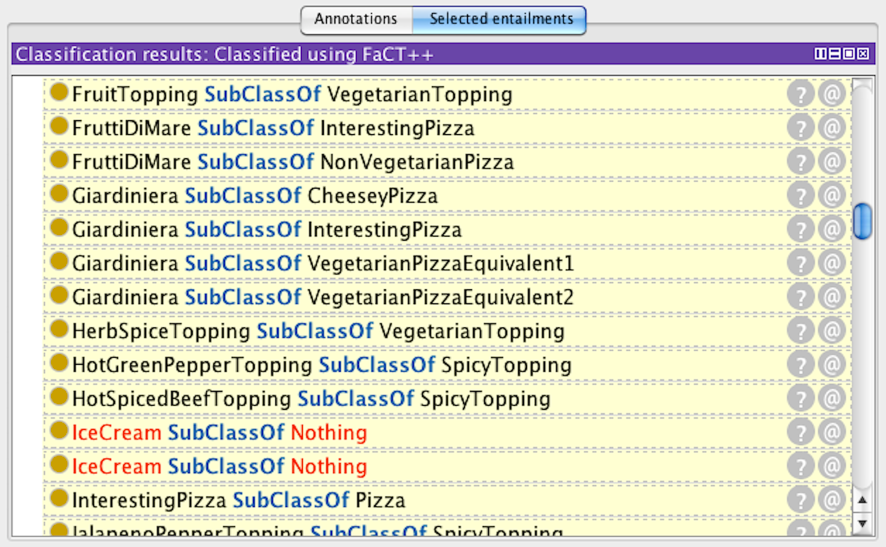
\includegraphics[width=0.9\textwidth]{img/entailment-tab.pdf}
\caption{Screenshot of the \enquote{Selected Entailments} tab in \protege}
\label{fig:selected-entaiments-tab}
\end{figure}


\subsection{Ontology publishing}

Ontologies that are available on the web may be published as \enquote{compiled} versions, which include the ontology and its entailments of some description. The OWL version of the National Cancer Institute (NCI) Thesaurus, for example, \enquote{includes inferred relationships}.\footnote{\url{http://evs.nci.nih.gov/ftp1/NCI\_Thesaurus/ReadMe.txt}} There is, however, no definition of what is regarded as an inferred relationship, how these relationships are determined, and what the selection criteria is. This may leave users wondering what kinds of information they are dealing with, and what implications this has for their understanding of the ontology. 

\subsection{Metrics and analytical applications}
Analytical applications that consider the number and types of entailments in order to infer ontology metrics depend on clearly defined finite entailment sets as the basis of their  measurements, i.e.\ \emph{what exactly} is measured. The entailment set used to generate metrics must be well defined and independent from a particular implementation or \emph{individual modifications} of results provided by the OWL API. From anecdotal evidence we know that developers of analytical tools frequently modify the results of the OWL API's \texttt{InferredAxiomGenerator} for use in their application, for example by removing entailments of the type \dlcn{A \subcls \top}. 

One such application is the use of entailment and justification metrics for the purpose of identifying ontology design styles \cite{mikroyannidi11aa} which ensures transparent and consistent measurements across different applications by clearly specifying the type of entailment set to be extracted. 

Another example is the counting of entailments which are lost in the debugging process of the OWL SafeMode tool \cite{scharrenbach11aa} in order to evaluate the quality of a repair step, which  requires a stable way of counting entailments that is not sensitive to the irregularities discussed above.

Finally, some approaches to ontology \emph{diffs}, that is, determining and quantifying the semantic and syntactic differences between two ontologies (e.g. two versions of an ontology), make heavy use of finite entailment sets. In these approaches the difference between two ontologies is measured based on the (countable) differences in their (finite) entailment sets. Gon\c{c}alves et al.\ \cite{goncalves11xz,Goncalves:2012kx} present several approximations to diffs which are based on increasingly complex types of entailment sets, such as entailed atomic subsumptions, subsumptions between complex class expressions already found in the ontologies, and a \emph{grammar diff} which generates new complex expressions to check for entailment.


\subsection{Imported and native entailments in BioPortal}
In a survey of 42 OWL and OBO ontologies from the NCBO BioPortal \cite{bail11jm}, we found that imported entailments (in the $(AI^{nim})^+$ set of atomic subsumptions of type $A \subcls B$ for satisfiable classes $A, B$) did in fact have a visible effect on the number of entailments found in those ontologies. In this corpus, the upper-level ontology \emph{Basic Formal Ontology (BFO)} \cite{grenon04aa} contributed significantly to the skewing of entailment counts. Table \ref{tab:bfo} shows an overview of the ontologies in the survey.

\begin{table}[htb]
\centering
\caption{Ontologies and imported entailments in the NCBO BioPortal.}\label{tab:bfo}	
\begin{tabu}{ccccccc}
\toprule
& \multicolumn{3}{c}{Importing BFO} & \multicolumn{2}{c}{Other imports} & \\
\cmidrule(r){2-4}\cmidrule(r){5-6}  
Ontologies & Total & Imported & Mixed & Total & Split & No imports \\
\midrule
42 & 7 & 3 & 4 & 7 & 5 & 28\\
\bottomrule
\end{tabu}
\end{table}

7 ontologies in the sample corpus imported BFO, of which 3 had no native entailments at all, but only 70 imported entailments which all originated from BFO. A further 4 ontologies had 70 imported entailments from BFO, plus additional entailments which were either native or imported from ontologies other than BFO. 

Additionally, a further 7 ontologies had imported entailments from ontologies other than BFO; for 5 of these, however, the imports could be attributed to the ontology being intentionally split up over several files with similar file names. Examples of these included the \emph{Chemical Information} ontology \cite{konyk2008aa}, which had 1 native entailment, 72 imported entailments from an ontology titled \enquote{cheminf-external}, and 3 entailments from \enquote{cheminf-core},  or the \emph{Semanticscience Integrated Ontology} (SIO),\footnote{\url{http://code.google.com/p/semanticscience/wiki/SIO}} which had imported entailments from an ontology called \emph{sio-core.owl}. 

Finally, 28 ontologies did not have any imported entailments at all, which could be either due to them having no imports, the imported ontology having no entailments that matched our criteria, or missing imports, which were ignored in the pre-processing stage when downloading the ontologies from BioPortal.

The example of the BioPortal ontologies shows how an analysis or comparison of ontologies based on the number of entailments and justifications needs to pay attention to their import structure; in the case of the BFO imports, the 3 ontologies which had only entailments from BFO would have appeared to have exactly the same number of entailments and justifications,  and thus might have been wrongfully classified as similar in terms of their expressivity and inferential power.


\section{Summary and conclusions}

In this chapter, we presented a discussion of the issues surrounding finite entailments sets for OWL ontologies. While the classification and computation of inferences is a standard reasoning task in the ontology engineering process, there exist ambiguities in ontology tools as to what constitutes the \enquote{set of entailments} of an ontology. We highlighted various design decisions to be made in order to clearly specify a non-ambiguous finite entailment set of an OWL ontology: how to deal with tautologies, whether to include asserted axioms, how to deal with transitive and non-strict subsumptions, and how to make the transition from nodes and edges in an abstract class graph to concrete sets of \emph{axioms} which are presented to a user or used in an OWL application. We also highlighted the problem of \emph{imported entailments} and how these can skew ontology metrics based on entailments, which was demonstrated using examples from a corpus of biomedical ontologies. The examples found in this chapter illustrate the wide scope of different entailment sets that can be specified depending on the application, ranging from minimal representations which are  suitable for user-facing applications, to exhaustive, yet finite, sets which may be used for analytical purposes.

The outcome of the work presented in this chapter is a deeper insight into what we mean by the \enquote{set of entailments} of an ontology, alongside a set of properties which can be used to precisely define a finite entailment set that is fit for a specific purpose. The main benefit of this set of properties is that it is defined from an \emph{application} perspective, which makes the effects of individual choices, such as whether to include indirect subsumptions, easier to understand for a user. Finally, we have made available a prototypical entailment generator on top of the OWL API, which allows the straightforward specification of finite entailment sets using a custom configuration file. The understanding and tools gained here lay the foundations for our discussion of the relations between justifications for entailment sets, which will be presented in the following two chapters.


\chapter{The justificatory structure of OWL ontologies}
\label{chap:structure}

In current ontology explanation tools, justifications are generally represented as individual entities in relation to a single entailment. However, this view neglects the rich relations that can be found between \emph{multiple} justifications for both single and multiple entailments of OWL ontologies. Previous surveys of OWL ontologies have shown that the majority of ontologies used in practice contain some entailment which has more than one justification, with many ontologies generating a few dozen and up to several hundred justifications for a single entailment \cite{bail10kb,horridge11ab,bail11jm}. 

Several properties of justifications, such as the number of justifications for an entailment, the size of justifications in an ontology, to which extent the ontology contains entailments which are entailed only by themselves, and which proportion of the ontology participates in justifications, all give us an insight into structural relationships in the ontology beyond standard metrics; we can say that the justifications make the \emph{implicit} relationships between the entitites and axioms of an ontology \emph{explicit}.

Further, justifications for a single or multiple entailments are not disjoint subsets of an ontology, but they often \emph{overlap} to a certain extent, sharing one or more axioms between them. This is relevant for both understanding as well as repairing the entailments of such justifications: shared axioms may\footnote{It is important to point out that a shared axiom does \emph{not} necessarily have to be an incorrect axiom; therefore, it is not guaranteed to be part of the hitting set that leads to a repair.} lead to a smaller hitting set, and therefore to a smaller repair for a set of entailments. Further, shared axioms may indicate common lemmas \cite{horridge09ct}, i.e.\ intermediate entailments, which can assist users in understanding (parts of) multiple justifications at the same time rather than treating each one independently, thus reducing the effort required to deal with multiple justifications.

In this chapter, we will introduce the notion of \emph{justificatory structure} of an OWL ontology. First, we present a categorisation of entailments based on the types of justifications they have in an ontology. We then lay out the motivation for analysing the relations between justifications in an ontology and define various structural aspects which may be of interest for ontology development and analysis. We introduce a graph-based representation of the justifications and entailments in an ontology and describe the generation and implementation of such a \emph{j-graph}. Along with Chapter 5, the work presented in this chapter constitutes the core of our research into the justificatory structure of OWL ontologies.


\section{Categories of justifications and entailments}
Following on from our discussion of different entailment sets in the previous chapter, we will now take a closer look at the different types and scenarios of justifications we encounter when analysing a finite entailment set of an ontology. While it is certainly the case that justifications are essentially equal---they are minimal entailing axiom subsets---we may treat them differently depending on the axioms they contain, and depending on their relation to the entailment in question.

\subsection{Self-justifications and self-supporting entailments}
Any justification which is simply the entailed axiom itself is classified as a \emph{self-justification}:
\begin{defn}[Self-justification]
A justification \J for an entailment \ent is a \emph{self-justification} if \J = $\{\eta\}$.
\end{defn}
We distinguish between entailments which have a self-justification in addition to other, more complex, justifications, and entailments which have \emph{only} a self-justification and no other justifications. Referring back to our discussion of finite entailment sets in Chapter 3, these entailments are commonly referred to as \enquote{asserted, but not inferred}; however, in order to avoid ambiguity caused by the word \emph{inferred} (as an asserted axiom can also be inferred from an ontology), we denote such as \emph{self-supporting} entailments: 
\begin{defn}[Self-supporting entailment]
An entailment \ent is \emph{self-supporting} if $\justseta = \{\{\eta\}\}$.
\end{defn}
There are different reasons why an entailment might have a self-justification \emph{in addition} to other justifications: 
\begin{compactenum}
\item The entailment was not asserted in the ontology to begin with, but explicitly added after it was found to be inferred. This could be in order to improve reasoner performance, to make the entailment visible to the \emph{developer} without using a reasoner (e.g.\ if the classification time is very high), or to make the inferences visible to \emph{end-users} in an ontology browser interface which does not support reasoning. 
\item The ontology modeller does not use a reasoner during the engineering process, thus is not aware that the subsumption is already entailed by the ontology, which means they might explicitly assert information which already exists implicitly.
\item The additional justifications are a side-effect of other axioms that were added to the ontology without the aim of causing the entailment, or with the aim of causing this \emph{and}  other entailments.
\end{compactenum}
Without additional information, such as axiom annotations or change logs of an ontology, it is not possible to tell the intentions of an ontology developer when adding an axiom which causes additional justifications or self-justifications. Moreover, developers may not even be \emph{aware} of the full impact that a modification has on the ontology. We therefore treat self-justifications and additional justifications on a purely logical level, disregarding the reasons for those multiple justifications.


\subsection{Atomic subsumption chains}

An \emph{atomic subsumption chain justification} in an ontology \O is a set of axioms of the type \dlax{A_{1} \subcls A_{2}},  \dlax{A_{2} \subcls A_{3}}, \ldots,  \dlax{A_{n-1} \subcls A_{n}} for an entailment \dlax{A_{1} \subcls A_{n}} where \dlcn{A_{i}} is a named class in \sig{\O}. It is clear to see that such an atomic subsumption chain justification of two or more axioms always represents an \emph{indirect} subsumption, which we have discussed in Chapter 3. Take, for example, the following ontology:
\begin{examp}
\begin{align*}
\O = \{ \dlax{A \subcls B}, \dlax{B \subcls C}, \dlax{A \subcls C} \}
\end{align*}
\end{examp}
The $A^{+}D^{-}$ entailment set of atomic subsumptions is the set $\{\dlax{A \subcls B}, \dlax{B \subcls C} \}$, whereas the  $(AD)^{+}$ entailment set is simply \O itself. While each entailment in $(AD)^{+}$ has a self-justification, the entailment \dlax{A \subcls C} has an additional atomic subsumption chain justification $\J=\{ \dlax{A \subcls B}, \dlax{B \subcls C} \}$. Despite \J being slightly less trivial than a self-justification, it is still simply based on the transitivity of subsumption. This implies that the interactions between axioms in the ontology (with respect to the class hierarchy) are trivial enough to be inferred by a structural reasoner.

Note that it is certainly possible for an entailment to have multiple atomic subsumption chain justifications. For example, adding the axioms $\{\dlax{A \subcls E}, \dlax{E \subcls C} \}$ to the above example would add another atomic subsumption chain justification for the entailment \dlax{A \subcls C}. 

In our survey of the justificatory structure of OWL ontologies presented in Chapter \ref{chap:survey}, we find that many ontologies which only contain self-justifications for direct subsumptions often have only atomic subsumption chain justifications for indirect subsumptions; that is, the information content of the ontology does not reach beyond its asserted class graph. 

\subsection{Complex justifications}
\label{sec:complexjusts}

Finally, we consider all justifications that are not self-justifications or atomic subsumption chains to be \emph{complex} justifications as opposed to \emph{trivial} self-justifications or atomic subsumption chain justifications. It is obvious that the level of complexity can vary strongly between justifications, depending on their size and the constructors used in their axioms. However, for the purpose of categorising justifications, such a coarse distinction between self-justifications, atomic subsumption chains, and \emph{other} justifications suffices.

It is clear to see that entailments can have both trivial and complex justifications. Assume we add further axioms to the above example ontology \O to obtain $\O' = \O \cup \{ \dlax{A \subcls \exists r.D, \exists r.D \subcls C}\}$. The entailment \dlax{A \subcls C} will then have another, complex, justification $\J = \{ \dlax{A \subcls \exists r.D, \exists r.D \subcls C}\}$ in addition to its self-justification and atomic subsumption chain justification.


\subsection{Categorising entailments and ontologies}

If we consider the categorisation of justifications from the point of view of their corresponding entailments, we can also arrange entailments and ontologies into a hierarchy based on their justification. This will be of use when analysing the justificatory structure of an ontology, as it allows us to decide which entailments and justifications to include in specific metrics. For example, when counting the numbers of justifications per entailment, we may want to treat trivial and non-trivial justifications separately in order to ensure that we are comparing equally relevant justifications. 

\begin{figure}
\centering
\begin{tikzpicture}[scale=1,->,auto=left]
  
%  \draw (-2,8.25) -- (6,8.25) -- (6,7.75) -- (-2,7.75) -- cycle;
% \draw (-2,7.5) -- (6,7.5) -- (6,7) -- (-2,7) -- cycle;
%  \draw (-2,8.25) -- (6,8.25) -- (6,7.75) -- (-2,7.75) -- cycle;
\node[align=left,text width=6cm] at (9,10) {Does $Justs(\eta)$ contain\ldots};
\node[align=left,text width=6cm] at (9,9) {a self-justification};
\node[align=left,text width=6cm] at (9,8) {an atomic subsumption chain j};
\node[align=left,text width=6cm] at (9,7.25) {a complex justification};
  
\node[draw=none] (root) at (2,9) {$\eta$};

\tikzstyle{every node} = [color=black,shape=circle,scale=0.5,draw]
  
\node (n) at (0,8)  {};
\node (y) at (4,8)  {};
\node (nn) at (-1,7.25)  {};
\node (ny) at (1,7.25)  {};
\node (yn) at (3,7.25)  {};
\node (yy) at (5,7.25)  {};

\tikzstyle{every node} = [draw=none]
\node[draw=none] (nnn) at (-1.5,6.5)  {x};

\node (nny) at (-0.5,6.5)  {$T_{4}$};	
\node (nyn) at (0.5,6.5)  {$T_{2}$};
\node (nyy) at (1.5,6.5)  {$T_{6}$};
\node (ynn) at (2.5,6.5)  {$T_{1}$};
\node (yny) at (3.5,6.5)  {$T_{5}$};
\node (yyn) at (4.5,6.5)  {$T_{3}$};
\node (yyy) at (5.5,6.5)  {$T_{7}$};



\draw (root) to node [swap]  {n} (n);
\draw (root) to node {y} (y);

\draw (n) to node [swap] {n} (nn);
\draw (n) to node {y} (ny);

\draw (nn) to node [swap]  {n} (nnn);
\draw (nn) to node {y} (nny);

\draw (ny) to node [swap]  {n} (nyn);
\draw (ny) to node {y} (nyy);

\draw (y) to node [swap]  {n} (yn);
\draw (y) to node {y} (yy);

\draw (yn) to node  [swap] {n} (ynn);
\draw (yn) to node  {y} (yny);

\draw (yy) to node [swap]  {n} (yyn);
\draw (yy) to node  {y} (yyy);


\end{tikzpicture}
\caption{A decision tree for categorising entailments.}
\label{fig:entailmenthierarchy}
\end{figure}

Figure \ref{fig:entailmenthierarchy} shows a decision tree for categorising an entailment based on its justifications. Given an entailment, the decision tree accepts a simple yes/no in the presence/absence of each type of justification, leading the entailment to be sorted into one of seven categories. We have labelled these categories with types $T_{1}$ through $T_{7}$ based on the number obtained if we regard the respective path in the decision tree as a (reversed) binary number. This results in uneven numbers for entailments which have self-justifications, and even numbers for those entailments that have only non self-justifications. 

This categorisation process can be applied to ontologies in order to rank them based on the justification types they contain (given some finite entailment set). This is of use when analysing the justificatory structure of an ontology, as it allows us to separate relevant ontologies (those that do contain entailments with complex justifications) from irrelevant ones (those that only contain trivial entailments). 



\section{Representing justifications as j-graphs}

In order to talk about the justificatory structure of an ontology, we require some way of representing structural aspects in an accessible way. The set of entailments, their justifications, and the axioms occurring in these justification can be easily represented as a graph, which allows us to describe aspects of justificatory structure using standard graph metrics such as the in- and out-degrees of nodes. In this section, we first define the terminology for different aspects of entailment and justification sets, which then allows us to define the \emph{justification graph} for a given set of entailments.


\subsection{J-graph definition}

Before defining j-graphs, we need to introduce the building blocks of these graph representations of justifications. Recall the notion of \justs which refers to the set of all justifications for the entailments in a particular finite entailment set of an ontology \O. Further, we define the set of all axioms occurring in all justifications for a particular entailment set:
\begin{defn}[Justification axioms]
\begin{align*}
\justax = \{\alpha \mid there~is~a~ \just \in \justs ~s.t.~\alpha \in \just\}
\end{align*}
\end{defn}
Based on our definitions of justification sets and justification axioms, we can now define the justification graph of an ontology \ont with respect to an entailment set \entset. A justification graph (\emph{j-graph}) \jgraph is a directed graph whose set of nodes is the union of the set of axioms \entset which are entailed by \O and the set \justax of axioms that participate in justifications for these entailments, together with the set of all justifications \justs. The graph does not contain axioms in \ont which are neither in the entailment set, nor in \justax, as these would not have any incoming or outgoing edges, thus not adding any information content.
\begin{defn}[Justification graph]
Given a set of entailments \entset, their justifications \justs, and justification axioms \justax, a \emph{justification graph} is a graph \jgraphdef where
\begin{compactitem}
\item $E_{1} =\{ (u,v) \in \entset \cup \justax \times \justs \mid u \in v\}$  and\\
\item $E_{2} =\{ (v,w) \in \justs\times \entset \mid v \in Justs(\ont, w) \}$.
\end{compactitem}
\end{defn}

\begin{figure}
\centering
\includedot[scale=0.6]{img/jgraph-example}
\caption{An example of a j-graph for justifications and entailments.}\label{fig:jgraphexample}
\end{figure}
Figure \ref{fig:jgraphexample} shows a j-graph of the small sample entailment and justification set in Example \ref{ex:jgraph}. As we can see in the example graph on nodes $a1$, $a10$, $a11$ and $a12$, an axiom node in the graph with an in-degree $\geq 1$ corresponds to an entailment in \entset. An axiom node with an out-degree $\geq 1$ correspond to an axiom in \justax; this node type is represented by nodes $a1$ through $a9$ in the example graph.

\begin{examp}\label{ex:jgraph}
\begin{align*}
j1 =& \{a1\} \models a1 \\
j2 =& \{a2, a3, a4\} \models a10\\
j3 =& \{a4, a5\} \models a11 \\
j4 =& \{a6, a7, a8\} \models a12\\
j5 =& \{a7, a8, a9\} \models a12\\
j6 =& \{a11\} \models a11
\end{align*}
\end{examp}

A self-justification corresponds to a cycle between an axiom node and a justification node (which, in turn, only has this one incoming edge), as justifications $j1$ and $j6$ show. A self-supporting entailment ($a1$ in the example graph) is represented by an axiom node which has no other incoming edges in addition to the cycle. 

Note that, while some j-graphs may be tripartite, an axiom node can be both in the set \justax and in \entset, i.e. have an outgoing edge to a justification node and an incoming edge from a justification node, as we can see from both axioms $a1$ and $a11$ in the example graph. Thus, a j-graph is bipartite, but not guaranteed to be tripartite.

There exists a \emph{unique} j-graph for every set of entailments, as the set of justifications for an entailment set is unique in an ontology, and the edges in the j-graph follow from these unambiguous relations.

Recall that the number of justifications for an entailment can potentially be exponential in the number of axioms in \ont. This affects the completeness of a j-graph for a given finite entailment set, as it may not be practical to compute \emph{all} justifications for \emph{all} entailments in the set. Despite the general feasibility of computing justifications, as shown in \cite{horridge11ab}, computing all justifications for a large finite entailment set can still require more time than an ontology user may consider practical. 

This means that we either need to sample a subset of entailments, or only generate a certain number of justifications for each entailment in the given entailment set---or both. While this omission of information is obviously problematic for users attempting to find a repair for \emph{all} justifications for a given entailment set, the only solution to such computational problems is incremental repair. Therefore, we only consider the j-graph for an entailment set to represent the particular set of entailments and justifications that could be processed, even if these are not all that exist in the ontology.


\subsection{J-graph generation}

\paragraph{Construction}

Generating a j-graph to represent the justificatory structure of an OWL ontology is a fairly straightforward process. First, all axioms in the union of the ontology and the selected entailment set \entset are labelled with a unique identifier $a_{i}$. We then compute the justifications for the entailments in \entset; the justifications are also labelled with unique identifiers $j_{k}$. The axiom labelling can also be performed on an existing set of justifications, which has no effect on the general structure of the process.

The j-graph is then constructed as follows: generate a node for each axiom in \justax and \entset (each justification in \justs) and label it with the respective identifier. For each justification node labelled $j_{k}$, generate an edge $(a_{i}, j_{k})$ for each axiom $a_{i}$ in the justification labelled $j_{k}$; this will create the edges representing the relation \enquote{axiom is used in justification}. For each entailment node $a_{i}$ with a justification $j_{k}$, generate an edge $(j_{k}, a_{i})$ which represents the relation \enquote{justification for entailment}. This construction requires only a single pass over all given justifications, axioms, and entailments.

	
\paragraph{Implementation}
\label{sec:jstrucimpl}
The above algorithm has been implemented using the OWL API version 3.2.4, and the JGraphT\footnote{\url{http://jgrapht.org/}} version 0.8.3 graph library for representing the j-graph. Construction of the graph on a set of existing justifications and entailments is performed quickly, with the average time to construct a graph being less than 10 seconds in a set of ontologies ranging from 2 to approximately 11,000 justifications.

%This concludes the introduction of the j-graph structure for representing justifications. Note that a graph representation may also lend itself as the basis justification-based interaction tool, since OWL users may already be familiar with graph-based ontology interaction tools, such as the OWLViz\footnote{\url{http://www.co-ode.org/downloads/owlviz/}} \protege plug-in.


\section{Justificatory structure}

Using the j-graph to describe relations between entailments, their justifications, and the axioms in the justifications, we can now discuss the various facets of the \emph{justificatory structure} of an OWL ontology. In a first instance, the justificatory structure provides additional ontology metrics; beyond these metrics, insights into the structure can support user understanding when coping with multiple justifications and/or multiple entailments. Further, in Chapter \ref{chap:understanding} we will introduce debugging techniques that are directly based on the interaction with the j-graph for a user-defined entailment set. 

Note that in this section we refer to \enquote{the entailments} and \enquote{the justifications} of an ontology, which requires a more precise specification. In what follows, we assume these entailments to be the $(AD)^{+}$ set of entailments which includes all asserted and inferred native, direct and indirect (non-tautologic) atomic subsumptions of the type \dlax{A \subcls B} for satisfiable classes $A, B$ which are entailed by \O, as this provides a clearly defined and natural starting point for exploring the properties of an ontology.

For ease of reading, we will use the terms \emph{justification}, \emph{axiom}, and \emph{entailment} interchangeably with \emph{justification node}, \emph{axiom node}, and \emph{entailment node} in the remainder of this chapter.

\subsection{Axiom properties}
\label{sec:arity}
The axioms occurring in justifications for a given set of entailments can have different properties, which we denote as axiom \emph{frequency}, \emph{impact}, and \emph{semantic relevance}. These three terms describe similar, but slightly distinct, measures of the effect an axiom in \justax has on a set of justifications and entailments. Figure \ref{fig:jgraph-arity} shows an example j-graph which exhibits different values of frequency, impact, and semantic relevance for the axiom node $a0$. Blank nodes labelled with \enquote{\ldots} indicate the existence of some additional axiom(s) occurring in a justification, respectively additional justification(s) for an entailment.

\begin{figure}
\centering
\includedot[scale=0.6]{img/jgraph-arityimpactsr}
\caption[J-graph illustrating axiom frequency, impact, semantic relevance.]{J-graph illustrating axiom frequency, impact, and semantic relevance. Axiom $a0$ has a frequency of 4, impact of 5, and semantic relevance of 3.} \label{fig:jgraph-arity}
\end{figure}

\subsubsection{Frequency}

The \emph{frequency}, also referred to as \emph{power} or \emph{arity}, of an axiom is the number of justifications (for a given entailment set \entset) the axiom occurs in. Removing an axiom with frequency $n$ from the ontology will break $n$ justifications for the entailments in \entset. Given that there can exist multiple justifications for an entailment, the frequency of the axioms in a set of justifications does not necessarily tell us how a removal would affect the actual \emph{entailments} of those justifications. In a j-graph, the frequency of an axiom node corresponds to its out-degree; an axiom with a frequency greater than 1 corresponds directly to a justification overlap of size 1 between the justifications the axiom occurs in:
\begin{defn}[Frequency]
$freq(u) =  \left|\lbrace v \mid  (u, v) \in E_{1}\rbrace \right|$ for $u \in \justax$.
\end{defn}
The axiom node $a0$ in Figure \ref{fig:jgraph-arity} has edges to four justifications ($j1$, $j2$, $j3$, $j4$); thus, $a0$ has a frequency of 4.

\subsubsection{Impact}

The \emph{impact} of an axiom is, in some sense, an extension of the axiom frequency. It refers to the number of \emph{entailments} in \entset that are directly affected by the axiom, as the axiom occurs in some justification for the entailments. Removing an axiom with an impact of $m$ from the ontology \emph{may} break $m$ entailments in \entset, assuming there are no other justifications for those $m$ entailments. Axiom frequency and impact coincide if each justification that the axiom occurs in has exactly one (distinct) entailment, and the impact is \emph{less} than the axiom frequency if the axiom occurs in multiple justifications for the same entailment. 

In a j-graph, the impact of an axiom node $u$ is defined as the sum of entailment nodes $w$ that  have an incoming edge from a justification node $v$ such that $(u, v) \in E_{1}$ and $(v, w) \in E_{2}$:
\begin{defn}[Impact]
$impact(u) =  \left| \lbrace w \mid  \exists v, w ~ s.t. ~ (u, v) \in E_{1}, (v, w) \in E_{2}\rbrace \right|$ for $u \in \justax$.
\end{defn}
The axiom node $a0$ in the j-graph in Figure \ref{fig:jgraph-arity} has an impact of 5, as it occurs in the justifications ($j1$, $j2$, $j3$, $j4$) for all five distinct entailments in the graph.

In the context of repairing a given set of entailments, we will need to consider the impact of axioms both with regard to the set of \emph{unwanted} as well as the set of \emph{wanted} entailments: removing a high-impact axiom from an ontology may break a large number, or all, unwanted entailments (e.g.\ unsatisfiable classes), but it may also lead to the removal of relevant information. Referring to our definitions of wanted and unwanted entailment sets in Section \ref{sec:wantedunwanted}, we can distinguish between the \emph{positive} and \emph{negative} impact of an axiom:
\begin{defn}[Positive and negative impact]
\begin{align*}
impact^{-}(\alpha) &= \left| \{\eta_{i} \mid \eta_{i} \in \entsetplus, \alpha \in JustAx(\entsetplus)\}\right| \\\
impact^{+}(\alpha) &= \left| \{\eta_{i} \mid \eta_{i} \in \entsetminus, \alpha \in JustAx(\entsetminus)\} \right| \\\
\end{align*}
\end{defn}	
In words, the negative impact of an axiom $\alpha$ is the number of \emph{wanted} entailments that are entailed by the justifications $\alpha$ occurs in, and the positive impact is the number of \emph{unwanted} entailments that are entailed by the justifications $\alpha$ occurs in. Note that the plus and minus signs for positive/negative impact and wanted/unwanted entailment sets are swapped, i.e. $impact^{-}$ refers to \entsetplus, and vice versa.

\subsubsection{Semantic relevance}
Finally, the \emph{semantic relevance} of an axiom, as defined by Kalyanpur \cite{kalyanpur06nm},  is the number of entailments that are \emph{dependent} on the axiom. Semantic relevance is closely related to the impact of an axiom, taking into account only those entailments that have no additional justifications (or \emph{only} justifications that contain the axiom). In the context of debugging a set of entailments, the semantic relevance of an axiom is the most meaningful of three axiom measures, as it gives a clear indication of the effect axiom removal will have on a set of entailments. Based on the definition given by Kalyanpur \cite{kalyanpur06nm} , the semantic relevance of an axiom node $u$ labelled with an axiom $\alpha$ in a j-graph is calculated as follows: 
\begin{defn}[Semantic relevance]
\begin{align*}
SR(u)  =  & \left| \{ w \mid \exists v, w ~ s.t. ~ (u, v) \in E_{1}, (v, w) \in E_{2} \wedge \not\exists v'   ~ s.t. ~ (v', w) \in E_{2} \wedge (u, v') \not\in E_{1} \}  \right|  \\
& ~ for ~ u \in \justax.
\end{align*}
\end{defn}

Axiom $a0$ in the j-graph in Figure \ref{fig:jgraph-arity} has a semantic relevance of 3, as it occurs in justifications ($j1$, $j2$, $j3$) for exactly three entailments ($a1$, $a2$, $a3$) which do not have any additional justifications that do not contain $a0$.

\subsubsection{Activity} 

We can define the \emph{activity} of an ontology \O with respect to a finite entailment set \entset  of \O. The activity corresponds to the total number of axioms that occur in justifications which are \emph{not} self-justifications, that is, the size of the subset of the ontology which actively participates in entailment: 
\begin{defn}[Activity]
\begin{align*}
activity(\O, \entset) = \dfrac{ \sum \left|\J_{i}\right| }{\left|\O\right|} ~ where~ \J_{i} \in \justs, ~ \J_{i} ~is ~not ~a ~self\!-\!justification.
\end{align*}
\end{defn}
Likewise, an \emph{active} axiom is an axiom which occurs in a justification that is not a self-justification:
\begin{defn}[Active axiom]
An axiom $\alpha \in \O$ is \emph{active} if $\alpha \in \J$ where $\J \in \justs, ~ \J$ is not a self-justification.
\end{defn}
Note that if we select the entailment set to be the deductive closure of the ontology, then the activity of the ontology is 1, since every axiom participates in the inference.


\subsection{Properties of justifications}

\subsubsection{Justificatory redundancy} 

Following on from the discussion of self-justifications and additional justifications, we can regard the number of justifications per entailment as an indicator of \emph{justificatory redundancy} in the ontology; it demonstrates \enquote{how often the same piece of information is expressed in different ways}. Justificatory redundancy is not to be confused with logical redundancy, as this would imply that it is possible to remove a set of axioms from the ontology without breaking any entailments.

In the j-graph, an axiom node with an in-degree $>1$ has redundant justifications; thus the in-degree (average, median, or maximum) of axiom-nodes in a j-graph is a metric for determining the level of justificatory redundancy in an ontology.


\subsubsection{Justfication size}

The \emph{size} of a justification is the number of axioms it contains; this corresponds to the in-degree of a justification node in the j-graph. Justification size gives us information about the use of entities in an ontology in two ways: first, large justifications can be caused by signatures which spread across multiple axioms, while small justifications indicate that the entities in the ontology are less connected. On the other hand, justifications with small numbers of axioms can also be caused by long axioms, that is, axioms containing many subexpressions, whereas justifications with many axioms may be caused by shorter axioms.

\subsection{Relations between justifications}

\subsubsection{Structural regularities} 
Two types of patterns can be identified in the context of the justificatory structure, namely \emph{structural isomorphism} between isomorphism and \emph{graph surface patterns}.

Justification isomorphism \cite{horridge11gj} describes a situation where the \emph{axioms} within a set of justifications share an identical structure; for example, the two justifications $\J_{1} =\{\dlax{A \subcls \exists r.B}, \dlax{\exists r.B \subcls C}\}$ \entails \dlax{A \subcls C} and $\J_{2} = \{\dlax{X \subcls \exists s.Y}, \dlax{\exists s.Y \subcls Z}\}$ \entails \dlax{X \subcls Z}  are isomorphic, as they have the same structure and only differ in the class and property names used. Justification isomorphism will be discussed in great detail in Chapter 5; for now we will focus on structural properties of the j-graph and treat justification axioms as \enquote{black boxes}.

A surface pattern is a structural similarity between sets of nodes and edges in the j-graph, such as subgraphs which match based on their node types and the numbers of ingoing and outgoing edges. Surface patterns in the j-graph reveal modelling similarities in the ontology, regardless of whether the axioms and expressions occurring in the pattern also interact in a similar way. Highlighting a pattern of this type may support user understanding of the modelling in the ontology, while it may also be an indicator for isomorphic justifications. In the example j-graph, the justifications $j4$ and $j5$ both have a similar structure (same in and out-degrees, two shared axioms), which may be an indicator for structurally isomorphic justifications.


\subsubsection{Graph components} 

A graph \emph{component} is a subset of nodes and edges which forms a disconnected subgraph. The number of components of a j-graph provides a measure for the disjointness of justifications in the ontology. The disjointness of justifications is thought to affect the justification computation process, which makes use of Reiter's Hitting Set Tree (HST) algorithm \cite{reiter87pb} for diagnosis. Recall that in the HST, the nodes are labelled with justifications and the paths constitute hitting sets across the justifications in the tree, i.e. minimal repairs for the justifications. Optimisations for the HST algorithm are mainly based on closing a branch in the tree if the path to it is labelled with a superset of an existing path, which is not possible if the justifications are disjoint. This is thought to lead to a rapid growth of the HST and have significant negative effects on the performance of computing all justifications for an entailment.

\subsubsection{Arbitrary justification overlap} 
\label{sec:overlap}

We have already touched upon the subject of justification overlap in the discussion of axiom frequency, as an axiom with a frequency greater than one simple corresponds to a single-axiom overlap between the justifications that the axiom occurs in. The concept of analysing frequently occurring \emph{axiom groups} in justifications for the purpose of finding a suitable repair was proposed by Schlobach in the early stages of justification-based explanation research \cite{schlobach05tf}. Due to a lack of an efficient implementation, however, the experimental analysis of such \emph{maximal arity cores} was restricted to single axioms, and has since not received any significant attention.

In the j-graph, arbitrary overlap between $n$ justifications corresponds to an intersection of the \emph{incoming neighbours} $N_{in}$ of the justification nodes with a cardinality greater than one. An intersection of size one corresponds to a single axiom with a frequency of $n$, thus, we are mainly interested in those overlaps which contain more than just one axiom.

Note that when we talk about overlaps between justifications there is no \emph{unique} overlap that a justification axiom occurs in. Instead, an axiom can occur in several overlaps of varying sizes between different justification sets. We can say that an overlapping set has two dimensions: its \emph{size}, which is the number of axioms in the overlap, and its \emph{frequency}, which has the same meaning as the frequency of a single axiom, that is, the number of justifications the overlapping axiom set occurs in.


\subsubsection{Root and derived justifications}

A special case of justification overlap are root and derived justifications, which we discussed in Section \ref{sec:rootderived}. Recall: a justification \jprime is derived from a justification \J if \J (the root justification) is a strict subset of \jprime. Due to the minimality of justifications, root and derived relations can only occur between justifications for \emph{multiple} entailments. In the j-graph, a root and derived relationship between two justification nodes is defined as a subset relation between the sets of incoming neighbours of the two nodes (where $N_{in}(v)$ denotes the set of nodes that have an outgoing edge to the node $v$):
\begin{defn}[Root and derived justifications]
A justification $v$ is \emph{derived} from a justification $v'$ if $N_{in}(v) \subset N_{in}(v')$, where $N_{in}(v) = \{u_{i}\}$ s.t. $(u_{i}, v) \in E_{1}$. A justification which is not derived from any other justification is a \emph{root} justification.
\end{defn}
Note that root and derived justifications were initially introduced as root and derived unsatisfiable classes. However, as the concept holds for arbitrary entailments, we can speak of root and derived entailments in the same way: a root unsatisfiable class is a class which has only root justifications, and likewise, an arbitrary entailment is a root entailment if it has only root justifications.
\begin{examp}
\begin{align*}
\O = \{ \dlax{A \subcls \exists r.B}, \dlax{\exists r.B \subcls C}, \dlax{B \subcls D}, \dlax{\exists r.D \subcls E} \}
\end{align*}
\label{ex:rootderivedentailments}
\end{examp}
In Example \ref{ex:rootderivedentailments}, the set comprising the first two axioms is a justification $\J_{1}$ for \dlax{A \subcls C}, while the set of all four axioms is a justification $\J_{2}$ for \dlax{A \subcls E}. Here, $\J_{1}$ is a root justification, and $\J_{2}$ is derived from $\J_{1}$. The two entailments are clearly related via the two axioms which constitute the root justification; we can say that $\J_{1}$ is the \emph{root} of the entailments, while the remaining two axioms act as a \emph{bridge} between them.

When confronted with a situation such as the justifications in Example \ref{ex:rootderivedentailments}, addressing the derived justification first may lead a user to modify or remove the bridging  axioms before the root axioms, thus only affecting the derived entailment. This would require the user to repair the root justification in another step, which would double the effort involved to repair both entailments. This example shows that when attempting to repair multiple entailments, addressing root justifications before derived justifications generally requires the inspection of fewer justifications, thus reducing user effort.


\subsubsection{Equality and inferential power}
Equality is another special case of justification overlap, where the same subset \J of axioms in an ontology \O is a minimal entailing set for several different entailments. We refer to the number of entailments for which \J is a justification as the \emph{inferential power} of \J, answering the question \enquote{how much can be expressed with how little?}. It is clear to see that for non-laconic justifications the inferential power depends largely on the size and complexity of the axioms in the justifications; we can easily construct an axiom with high inferential power by creating a large conjunction of subexpressions, where only some of the subexpressions are relevant for a given entailment. On the other hand, this is not the case for laconic justifications, as these will not contain any superfluous information with respect to an entailment.

For justification equality, the j-graph representation has clear benefits over a representation of multiple justifications as lists of axiom sets. Several justifications for multiple entailments which are equivalent are simply represented by a single justification node; the inferential power of a justification corresponds to its out-degree in the j-graph. 


\section{Summary and conclusions}

This chapter introduced the notion of the justificatory structure of OWL ontologies, defined a graph-based representation of the justificatory structure, and gave a brief overview of the implementation of a generator for such graphs. We discussed a strategy for categorising justifications and entailments based on their relevance, the occurrence of multiple justifications in OWL ontologies, and the various properties associated with entailments and their justifications. Some of these measurements, such as the numbers and sizes of justifications for a finite entailment set of an ontology, or the activity of an ontology, that is, the proportion of ontology axioms that occur in justifications for an entailment set, give us insight into the implicit structure of an ontology, thus extending the standard metrics used to describe OWL ontologies.

Other structural aspects are based on relations between multiple justifications, such as shared axioms between justifications. Justifications for both single and multiple entailments may share some axioms, i.e. the justifications \emph{overlap} to a certain extent. Justification overlaps are key in finding good repairs for a set of justifications, as they may lead to a smaller repair (i.e. hitting set) over the justifications.  Furthermore, overlapping justification subsets may also support users in \emph{understanding} multiple justifications by generating lemmas, that is, intermediate entailments, which summarise a recurring set of axioms. In the case of multiple entailments, relations such as root and derived and justification equivalence even seem crucial to reducing user effort for justification understanding and repair, as they highlight the actual (number of) reasons for the entailments to hold. An in-depth discussion of how justificatory structure can be exploited in the debugging process will follow in Chapter \ref{chap:understanding}; for now, we will continue our exploration of justificatory structure by focussing on one particular structural property, namely equivalence relations over justifications in the form of different isomorphisms.

\chapter{Justification isomorphism}
\label{chap:iso}

In the previous chapter, we introduced the justificatory structure of ontologies and treated the axioms as anonymous \enquote{building blocks} of justifications, without paying consideration to the subexpressions occurring in them. In this chapter, we will go one step further and take into account the logical form of the \emph{axioms} occurring in justifications. 

Given the high expressivity of modern ontology languages, such as OWL, there is the possibility for great diversity in the logical content of ontologies. The fact that many naturally occurring entailments have multiple justifications indicates that ontologies often overdetermine their consequences. However, the multiplicity of justifications might be due mostly to diverse \emph{material}, not \emph{formal}, grounds for an entailment. That is, the logical form of these multiple reasons could be less diverse than their numbers suggest. Such logical similarity indicates that it is possible group justifications into sets of structurally similar ones by the means of an equivalence relation.

A well-known syntactical equivalence relation in OWL is \emph{structural equivalence}. The OWL Structural Specification\footnote{\url{http://www.w3.org/TR/owl2-syntax}} states the condition for two OWL objects (named classes, properties, or instances, complex expressions, or OWL axioms) to be structurally equivalent: in short, it defines the objects to be equivalent if they contain the same names and constructors, regardless of ordering and repetition (in an unordered association). The OWL API implements this notion of structural equivalence by default.

A second equivalence relation is \emph{justification isomorphism}\footnote{Note that, in the spirit of consistent naming, we will use the term \enquote{isomorphism} for the newly introduced equivalent relations despite their not being isomorphisms (i.e. bijective mappings) in the true sense.} which was first introduced in a study of the cognitive complexity of justifications \cite{horridge11gj}: two justifications are isomorphic if they are structurally identical,\footnote{Modulo structural equivalence.} i.e.\ the axioms contain the same \emph{types of} class expressions and only differ in the class, property and instance names. The following example shows two justifications $\J_{1}$ and $\J_{2}$ which we consider to be isomorphic:


\begin{examp}[Isomorphic justifications]
\begin{align*}
\J_{1} &= \{ A \sqsubseteq B \conj \exists r.C, B \conj \exists r.C \sqsubseteq D\} \models A \sqsubseteq D\\
\J_{2} &= \{ E \sqsubseteq B \conj \exists s.F, B \conj \exists s.F  \sqsubseteq D\} \models E \sqsubseteq D
\end{align*}
\end{examp}

It is straightforward to see that in the above justifications the class \dlcn{A} in $\J_{1}$ can be mapped to \dlcn{E} in $\J_{2}$, the property \dlcn{r} to \dlcn{s}, and the class \dlcn{C} to \dlcn{F} in order to obtain identical justifications.

While justification isomorphism helps to eliminate the effects of diverging class, property, and instance names, we can also identify types of justifications which may be considered to be very similar despite their use of different constructors:

\begin{examp}
\label{ex:subex}
\begin{align*}
\J_{1} &= \{A \sqsubseteq B \conj C, B \conj C \sqsubseteq D \} \models A \sqsubseteq D  \\ 
\J_{2} &= \{ A \sqsubseteq \exists r.C, \exists r.C  \sqsubseteq D\} \models A \sqsubseteq D
\end{align*}
\end{examp}
In this example, the semantics of the complex class expressions $B \conj C$ in $\J_{1}$ and $\exists r.C$ in $\J_{2}$  are not relevant for the respective entailment; their occurrences in the justifications and their entailments can be replaced by freshly generated class names without affecting the entailment relation. Such a substitution, in turn, would make the two justifications isomorphic.

Likewise, justifications of different lengths may be considered similar if their general structure of reasoning is identical:
\begin{examp}
\begin{align*}
\J_{1} &= \{A \sqsubseteq B, B \sqsubseteq C \} \models A \sqsubseteq C  \\ 
\J_{2} &= \{ A \sqsubseteq B, B \sqsubseteq C, C \sqsubseteq D \} \models A \sqsubseteq  D
\end{align*}
\end{examp}

These two justifications clearly require the same form of reasoning from a user which means we may consider them to be structurally similar in some way. Strict isomorphism only applies to justifications which contain the same number of axioms; it does not cover situations like one shown above. However, for the purpose of structuring sets of justifications and analysing the logical diversity of a corpus of justifications, capturing those kinds of similarities illustrated in the above examples would be highly desirable. 

In this chapter, we introduce two new equivalence relations, \emph{subexpression-isomorphism} \sisom and \emph{lemma-isomorphism} \lisom,  between justifications based on the subexpressions of their axioms and axiom subsets, respectively, and show how these equivalence relations can be used to determine the logical diversity of a set of justifications. We present an algorithm to detect such equivalence relations and discuss their practical implementation as part of the framework for analysing the justificatory structure of OWL ontologies.


\section{Isomorphism}

Justification isomorphism was first introduced as a way to reduce sampling bias in a user study to validate a model for the cognitive complexity of OWL justifications \cite{horridge11gj}. When studying the cognitive complexity of justifications, we can assume that ontology users will perceive isomorphic justifications as equally difficult to understand, taking into account some variation caused by the complexity of class names and domain knowledge. The ontology corpus from which the justifications in the complexity study \cite{horridge11gj} were sampled was reduced from 64,800 to 11,600 non-isomorphic justifications, thus eliminating the risk of sampling bias caused by presenting users a series of structurally identical justifications. Recall that a justification \J is always defined with respect to a particular entailment \ent; thus, we will use the notation $(\J, \eta)$ to refer to a justification-entailment pair. Justification isomorphism is defined as follows:

\begin{defn}[Justification isomorphism]
Two justifications ($\J_{1},\eta_{1}$), ($\J_{2},\eta_{2}$) are \emph{isomorphic} (($\J_{1},\eta_{1}$) $\isom$ ($\J_{1},\eta_{1}$)) if there exists a bijective renaming $\phi$ which maps class, property, and instance names in $\J_{1}$ and $\eta_{1}$ to class, property, and instance names in $\J_{2}$ and $ \eta_{2}$, respectively, such that $\phi(\J_{1}) = \J_{2}$ and $\phi(\eta_{1}) = \eta_{2}$. 
\end{defn}
\paragraph{Remarks}
\begin{compactenum}
\item The relation \isom is symmetric, reflexive and transitive, from which it follows that \isom is an equivalence relation and thus partitions a set of justifications. Proofs are omitted as these properties are straightforward to see.
 \item Justification isomorphism preserves the numbers and types of axioms and subexpressions in the justifications:
\begin{compactenum}
\item If $\J_{1} \isom \J_{2}$ then $\left|\J_{1}\right| = \left|\J_{2}\right|$.
\item Since the mapping $\phi$ is bijective, we also have $\J_{1} \isom \J_{2} $ implies that $\left|sig(\J_{1})\right| = \left|sig(\J_{2})\right|$.
\item The sets of logical constructs used in $\J_{1}$ and $\J_{2}$ coincide.
\end{compactenum}
\end{compactenum}

\section{Subexpression-isomorphism}

From the above definition of isomorphism it follows that only justifications which have the same number and types of axioms and subexpressions can be  isomorphic. It is easy to see, however, that justifications can have a similar structure despite their use of different class expressions, as demonstrated in Example \ref{ex:subex}. Furthermore, obfuscating complex expressions which can be substituted by propositional variables reduces superfluous clutter in a justification, thus improving the readability of a justification akin to laconic justifications. This motivates a notion of \emph{subexpression-isomorphism}, an equivalence relation which allows not only the mapping of class names, but also that of complex subexpressions.

The idea of finding similarities between concepts in description logics has been widely explored in the work on \emph{unification} and \emph{matching}, e.g.\ \cite{baader98yt,baader99ai,baader09je}, for the purpose of detecting redundant class descriptions in ontologies. Given two class expressions $C$ and $D$, a \emph{unification problem} $C \equiv^{?} D$ asks whether there exists a \emph{substitution} $\sigma$, that is, a mapping from a set of named classes in $C$ into the set of class expressions in $D$, such that $\sigma(C) \equiv \sigma(D)$. The aim of unification is to find a suitable substitution $\sigma$ which maps atomic classes $C$ to (possibly non-atomic) classes in $D$ such that the two classes are made equivalent. 

While the basic idea behind subexpression-isomorphism is based on unification and matching, the concepts are not directly applicable to the given problem of matching justifications. In our case, the inputs are of different shape from the matching problem: the goal is to unify two sets of axioms and the corresponding entailments, rather than matching a single class expression (a class \emph{pattern}) which contains variables to a class expression. That is, we attempt to identify pairs of possibly complex class expressions that, when replaced with names, result in isomorphic justifications. This means that the substitution mechanism as used in unification is not applicable.

We therefore introduce a \emph{justification template} $\jtemplate$, which functions as the \emph{unifying justification} for the isomorphic justifications and \emph{two} substitutions $\phi_{1}, \phi_{2}$ for use in subexpression-isomorphism. We will use freshly introduced entity names $x_{i}$ for the named classes, properties, and instances in a template \jtemplate. In order for subexpression-isomorphism to be transitive, the justifications will have to fulfil certain side-conditions, which will be used in the proof of Proposition \ref{prop:trans}:
\begin{compactenum}[\bfseries S1]
\item For any $C$ in the range of $\phi{1}$ ($\phi{2}$), $C$ is not equivalent to \thing.
\item For any $C$ in the range of $\phi{1}$ ($\phi{2}$) is satisfiable in a \emph{single} element of some interpretation, that is, there is some $I$ such that $\left|C^{I} \right| = 1$.
\item For any $C_{1}$, $C_{2}$ in the range of $\phi^{ac}_{1}$ ($\phi^{ac}_{2}$, respectively), it must hold that $\sig{C_{1}} \cap \sig{C_{2}} = \emptyset$ and $\sig{C_{i}} \cap \sig{\Theta} = \emptyset$, that is, the expressions in the domain and the range of the mappings must be pairwise signature disjoint.
\end{compactenum}

\begin{defn}[Subexpression-isomorphism]
\label{def:siso}
Two justifications ($\J_{1},\eta_{1}$), \\
($\J_{2},\eta_{2}$) are \emph{s-isomorphic} (($\J_{1},\eta_{1}$) \sisom ($\J_{2},\eta_{2}$)) if there exists a justification \emph{template} ($\jtemplate, \eta$) and two injective substitutions $\phi_{1}, \phi_{2}$ satisfying \textbf{S1} to \textbf{S3}, such that 
\begin{compactenum}
\item $\jtemplate \models \eta$
\item $\phi_{1}(\jtemplate)=\J_{1} $ and $\phi_{2}(\jtemplate) = \J_{2}$
\item $\phi_{1}(\eta)=\eta_{1}$ and $\phi_{2}(\eta)=\eta_{2}$.
\end{compactenum}
The mappings $\phi_{1}$ and $ \phi_{2}$ map class, property, and instance names in the template ($\jtemplate, \eta$) to subexpressions of ($\J_{1}$, $\eta_{1}$) and ($\J_{2}, \eta_{2}$), respectively.
\end{defn}
Note that in order to be s-isomorphic, the justifications may differ in the number of subexpressions. As with strict isomorphism, however, they must have the same number of axioms: $\J_{1} \sisom \J_{2} \rightarrow \left|\J_{1}\right| = \left|\J_{2}\right|$. 

\begin{prop}
\label{prop:siso}
S-isomorphism is a more general case of strict isomorphism: $\J_{1} \isom \J_{2} \rightarrow   \J_{1} \sisom \J_{2} $.
\end{prop}


\begin{proof}
Let $(\J_{1}, \eta_{1}) \isom (\J_{2}, \eta_{2})$ via a mapping $\phi$. Then we can consider a  template $\jtemplate$ to correspond to $\J_{1}$, the mapping $\phi_{1}$ is the identity relation $id$ which maps $\J_{1}$ to itself, and $\phi_{2}$ corresponds to the mapping $\phi$ used for strict isomorphism. Thus $\J_{1} \isom \J_{2}$ then $\J_{1} \sisom \J_{2}$.
\end{proof}


\begin{prop}
\label{prop:trans}
The relation \sisom is reflexive, transitive and symmetric for description logics without nominals up to \dl{SRIQ}.
\end{prop}

\begin{proof} Reflexivity and symmetry of the relation are straightforward to see; therefore we will only prove the transitivity of subexpression-isomorphism for logics not containing nominals.

Let $(\J_{a}, \eta_{a}) \sisom (\J_{b}, \eta_{b}) $ via $\phi^{ab}_{1}, \phi^{ab}_{2}, (\jtemplate_{ab}, \eta_{ab})$ and $(\J_{b}, \eta_{b}) \sisom (\J_{c}, \eta_{c}) $ via $\phi^{bc}_{1}, \phi^{bc}_{2}, (\jtemplate_{bc}, \eta_{bc})$, respectively. We aim to show that given this case it is always possible to construct two mappings $\phi^{ac}_{1}, \phi^{ac}_{2}$ and a template  $(\jtemplate_{ac}, \eta_{ac})$, such that $(\J_{a}, \eta_{a}) \sisom (\J_{c}, \eta_{c}) $ via $\phi^{ac}_{1}, \phi^{ac}_{2}$ and $(\jtemplate_{ac}, \eta_{ac})$, as illustrated in Figure \ref{fig:transitivity}. In what follows, we will first describe the construction of  $(\jtemplate_{ac}, \eta_{ac})$ and $\phi^{ac}_{1}, \phi^{ac}_{2}$. We will then show that the entailment relation $\jtemplate_{ac} \models \eta_{ac}$ holds by describing the steps to extend any model $I_{ac}$ for $\jtemplate_{ac}$ to a model of $\eta_{ac}$ by constructing a model $I_{a}$ of $\J_{a}$ (or $I_{c}$ of $\J_{c}$, respectively)

\begin{figure}
\centering
\begin{tikzpicture}
  [scale=1,->,auto=left,every node/.style={draw=none, fill=none}]

  \node (tab) at (3.5,9) {$ (\Theta_{ab}, \eta_{ab})$};
  \node (tbc) at (8.5,9) {$(\Theta_{bc}, \eta_{bc})$};
  \node (tac) at (6,10.5) {$(\Theta_{ac}, \eta_{ac})$};
    
  \node (ja) at (1,8) {$(\J_{a}, \eta_{a})$};
  \node (jb) at (6,8) {$(\J_{b}, \eta_{b}) $};
  \node (jc) at (11,8) {$(\J_{c}, \eta_{c}) $};

  \draw [bend right] (tab) to node {$\phi^{ab}_{1}$} (ja);
  \draw [bend left] (tab) to node [swap] {$\phi^{ab}_{2}$} (jb);
  \draw [ bend right] (tbc) to node {$\phi^{bc}_{1}$} (jb);
  \draw [bend left] (tbc) to node [swap]  {$\phi^{bc}_{2}$} (jc);
  
  \draw [bend right] (tac) to node [swap]  {$\phi^{ac}_{1}$} (ja);
  \draw [bend left] (tac) to node {$\phi^{ac}_{2}$} (jc);


  \draw [<->, dashed] (ja) to node {$\sisom$} (jb);
  \draw [<->, dashed] (jb) to node [swap] {$\sisom$} (jc);
  \draw [<->, dashed, bend right] (ja) to node {$\sisom$} (jc);
    
\end{tikzpicture}
\caption[Three justifications which are s-isomorphic via transitivity.]{Graph representing the relations between three justifications which are subexpression-isomorphic via transitivity.}\label{fig:transitivity}
\end{figure}

First, in order to construct $\Theta_{ac}$ and $\eta_{ac}$, take $\J_{b}, \eta_{b}$ and label each position $p$ in their parse trees\footnote{We use standard notations: $\J|_{p}$ is the subtree/subexpression of \J at position $p$, and $\J[s \rightarrow t]$ the tree obtained by replacing, in \J, the subtree at position $s$ with $t$.} with variables
\begin{compactitem}
\item $(x, ab)$ if $\phi^{ab}_{2}(x) = \J_{b}|_{p}$ and $\jtemplate_{ab}|_{p} = x$
\item $(x, bc)$ if $\phi^{bc}_{1}(x) = \J_{b}|_{p}$ and $\jtemplate_{bc}|_{p} = x$
\end{compactitem}
and the analogue for $\eta_{b}$, i.e.\ we mark nodes in the parse trees of $(\J_{b}, \eta_{b})$ with variables from $(\Theta_{ab}, \eta_{ab})$ if applicable. Please note that a node in the parse trees may be labelled with two such variable labels $(x, ab), (x', bc)$ if $\phi^{ab}_{2}(x) = \phi^{bc}_{1}(x') = \J_{b}|_{p}$.

Now $(\jtemplate_{ac}, \eta_{ac})$ is obtained from this labelled tree by 
\begin{compactitem}
\item removing all subtrees below nodes labelled with variables $(x,\ldots)$ 
\item turning the variables $x$ in these labels $(x,\ldots)$ into leaf nodes (giving precedence to $(x,ab)$ in the presence of two labels), and 
\item serialising the result into a justification and entailment template $(\jtemplate_{ac}, \eta_{ac})$.
\end{compactitem}

We then construct the mappings $\phi^{ac}_{1}$ and $\phi^{ac}_{2}$: if a variable $x$ in $(\jtemplate_{ac}, \eta_{ac})$ originates from a labelling $(x,ab)$ in $\J_{b}$ at position $p$, then 
\begin{compactitem}
\item $\phi^{ac}_{1}(x) = \phi^{ab}_{2}(x)$ and
\item $\phi^{ac}_{2}(x) = \J_{b}|_{p} [t_{j} \rightarrow \phi^{bc}_{2}(y_{j})]$ for $t_{j}$ the positions in $\J_{b}|_{p}$ that are labelled with $(y_{j}, bc)$.
\end{compactitem}
and the analogue for variables originating from labellings $(x, bc)$, and for $\eta_{b}$.

Finally, we need to ensure that the resulting $\jtemplate_{ac}$ indeed entails $\eta_{ac}$. We prove that every model $I_{ac}$ for $\Theta_{ac}$ is a model for $\eta_{ac}$ by first showing that, for $I_{ac}$ a model of $\Theta_{ac}$, we can extend $I_{ac}$ to a model $I_{a}$ for $\J_{a}$ (or the analogue for $I_{c}, \J_{c}$). Given a model $I_{ac} = (\deltaiac, \dotiac)$ of $\jtemplate_{ac}$, we construct $I_{a}$ such that for every $x \mapsto C$ in $\phi^{ac}_{1}$ it holds that $C^{I_{a}} = x^{I_{ac}}$. 

Recall that the expressions in $\J_{a}$ have to fulfil the side conditions \textbf{S1--S3} mentioned above in order for this construction to be possible. The construction steps for $I_{a}$ then are as follows:
\begin{compactitem}
\item Take a model $I_{ac}$ of $\Theta_{ac}$.
\item For each $x \mapsto C$ consider the extension of $x^{I_{ac}} = \{a_{1}, a_{2}, \ldots\}$ where $\left| x^{I_{ac}}\right| = k$ (possibly infinite) and take a model $I$ of $C$ with $\left|C \right| = 1$ to create $k$ \enquote{copies} of $I$. This means we obtain a copy $I_{i}$ of $I$ for each $a_{i} \in x^{I_{ac}}.$
\item For each $a_{i} \in x^{I_{ac}}$, take $I_{i}$ (the $i$-th copy of $I$) and replace the single element $z_{i}$ in $C^{I_{i}}$ with $a_{i}$; in particular, replace $(z_{i}, b) \in r^{I_{i}}$ with $(a_{i}, b)$.
\item Finally, unite the $I_{ac}$ and the models $I_{i}$ created in this way by taking their disjoint union \cite[p 191]{lutz02gy}, that is, the union of the domains and the union of the respective extensions in the models, to obtain a model $I_{a}$ for $\J_{a}$.
\end{compactitem}

With the above steps we have shown that, given any model $I_{ac} \entails \jtemplate_{ac}$, it is possible to construct a model $I_{a}$ such that $I_{a} \models \J_{a}$. Since $\J_{a} \models \eta_{a}$, it also holds that $I_{a} \models \eta_{a}$. 
By construction we know that, for every variable $x$ in $\Theta_{ac}$ or $\eta_{ac}$, it holds that $(\phi^{ac}_{1}(x))^{I_{a}} = x^{I_{ac}}$ and thus $I_{ac} \models \eta_{ac}$. This means that every model $I_{ac}$ for $\Theta_{ac}$ is a model for $\eta_{ac}$, thus the entailment relation $\Theta_{ac} \models \eta_{ac}$ holds. We have therefore shown that we can always construct a template $(\jtemplate_{ac}, \eta_{ac})$ for the justifications $\J_{a}$ and $\J_{c}$, and thus $\J_{a} \sisom \J_{c}$.
\end{proof}

In order to demonstrate the non-transitivity of subexpression-isomorphism in the presence of nominals, we consider a simple counter-example:

\begin{align*}
\O = \{ C \sqsubseteq \{a\},  C \sqsubseteq \{b\}, \{a\} \conj \{b\} \conj \leq 1 r.C \sqsubseteq D\}
\end{align*}
which entails $\eta = C \sqsubseteq D$. The only justification for $\eta$ is the set of all axioms in $\O$. Now modify the ontology to obtain 
\begin{align*}
\O_{a} = &  \{ C \sqsubseteq A,  C \sqsubseteq \{b\}, A \conj \{b\}~ \conj \leq 1 r.C \sqsubseteq D\}\\
\O_{b} = & \{ C \sqsubseteq \{a\},  C \sqsubseteq B, \{a\} \conj B ~\conj \leq 1 r.C \sqsubseteq D\}.\\
\end{align*}
Both $\O_{a}$ and $\O_{b}$ entail $\eta$, and we have that $\O \sisom \O_{a}$ and $\O \sisom \O_{b}$. However, if we substitute the nominals $\{a\}$ and $\{b\}$ with atomic concepts $X$ and $Y$, respectively, in the template
\begin{align*}
 \jtemplate = \{ C \sqsubseteq X,  C \sqsubseteq Y, X \conj Y \conj \leq 1 r.C \sqsubseteq D\}
 \end{align*}
we find that the conjunct $\leq 1 r.C$ is no longer satisfied by all instances of $C$ (and thus $x$ and $y$) and $\jtemplate$ does not entail $C \sqsubseteq D$. This shows that the relation \sisom is not transitive in the presence of nominals.

Finally, note that the substitutions $\phi_{1}$ and $ \phi_{2}$ are injective, but not surjective. As we have shown in the proof of \ref{prop:trans}, injectivity of the mappings is a condition for the transitivity of subexpression-isomorphism. However, the mappings are not surjective, as the set of subexpressions in the justifications  $\J_{1}$ and $\J_{2}$ can be of higher cardinality  than the set of class names in \jtemplate (unless the justifications themselves contain no complex expressions). This is illustrated by the following counter-example of non-surjective mappings: 
\begin{examp}
\begin{align*}
\J_{1} &= \{A \sqsubseteq B, B \sqsubseteq C \}  \\ 
\J_{2}  &= \{ A \sqsubseteq B \conj \exists r.C, B \conj \exists r.C   \sqsubseteq D\}\\
\jtemplate &=  \{x_{1} \sqsubseteq x_{2}, x_{2} \sqsubseteq x_{3} \}  \\ 
\phi_{1} &= \{ x_{1} \mapsto A, x_{2} \mapsto B, x_{3} \mapsto C\}\\
\phi_{2} &= \{ x_{1} \mapsto A, x_{2} \mapsto B \conj \exists r.C, x_{3} \mapsto D\}
\end{align*}
\end{examp}

The set of \emph{all} subexpressions of $\J_{2}$ is $\{A, B, \exists r.C, B \conj \exists r.C, D\}$. $\phi_{2}$ maps only to a subset of these subexpressions; there exists no mapping for the \enquote{smaller} expressions $B$ and $\exists r.C$. This shows that a substitution $\phi$ can be non-surjective.

Despite the mappings being non-surjective, we require each subexpression to either have a corresponding variable in \jtemplate which maps to it directly, or to occur as part of a larger subexpression which has a corresponding variable in \J. This guarantees that the isomorphic justifications have the same number of subexpressions which correspond to variables in \J.


\subsection{Preferred templates}

Given a pair of isomorphic justifications, the template \jtemplate and the substitutions $\phi_{1}, \phi_{2}$ are not necessarily unique; there can be multiple possible substitutions, as demonstrated in Example \ref{ex:preferredsubs}. The substitutions differ in the level of \emph{granularity}, that is, how large a subexpression a variable in \jtemplate is mapped to. Keeping in mind our eventual goal of helping users cope with justifications, we introduce \emph{preferred templates} which reduce the amount of unnecessary detail in a justification template as far as possible. This means that a preferred template $\Theta_{p}$ contains the smallest possible expressions, i.e.\ atomic variable names, where possible. In turn, a substitution $\phi_{i}$ maps a variable in a preferred $\jtemplate_{p}$ to the largest possible subexpression in its corresponding justification $\J_{i}$. Assuming that $\jtemplate, \jtemplate_{p}$ are valid templates for a pair of justifications $(\J_{1}, \eta_{1})$ $(\J_{2}, \eta_{2})$, and $sig(\Theta) \cup sig(\eta)$ is the set of all variables occurring in a template $(\jtemplate, \eta)$, we can define preferred templates as follows:
\begin{defn}[Preferred template]
A template $(\Theta_{p}, \eta_{p})$ is a \emph{preferred template} if there is no template $(\jtemplate, \eta)$ such that $(sig(\jtemplate) \cup sig(\eta)) \subset (sig(\jtemplate_{p}) \cup sig(\eta_{p}))$.
\end{defn}

We illustrate the concept of preferred templates with the following example:
\begin{examp}
\begin{align*}
\J_{1}  &= \{A \sqsubseteq B \conj C\conj D, B\conj C\conj D \sqsubseteq E \}  \\ 
\J_{2}  &=  \{ A \sqsubseteq B \conj \exists r.C, B \conj \exists r.C   \sqsubseteq D\}\\
\jtemplate  &=  \{x_{1} \sqsubseteq x_{2} \conj x_{3}, x_{2} \conj x_{3}\sqsubseteq x_{4} \}  \\ 
\phi_{1}  &=  \{ x_{1} \mapsto A, x_{2} \mapsto B, x_{3} \mapsto C \conj D, x_{4} \mapsto E\}\\
\phi_{2}  &= \{ x_{1} \mapsto A, x_{2} \mapsto B, x_{3} \mapsto \exists r.C, x_{4} \mapsto D\}
\end{align*}\label{ex:preferredsubs}
\end{examp}
In the above example, the template \jtemplate contains a conjunction $x_{2} \conj x_{3}$, which means that only parts of the conjunctions in the justifications $\J_{1}$ and $\J_{2}$ are substituted by variables. It is straightforward to see, however, that there exists an alternative $\jtemplate_{p}$ and substitutions $\phi_{1}'$, $\phi_{2}'$ which substitute larger expressions in the two justifications:

\begin{examp}
\begin{align*}
\jtemplate_{p}   &=  \{x_{1} \sqsubseteq x_{2}, x_{2} \sqsubseteq x_{3} \}  \\ 
\phi_{1}'  &=  \{ x_{1} \mapsto A, x_{2} \mapsto B\conj C\conj D, x_{3} \mapsto E\}\\
\phi_{2}'  &= \{ x_{1} \mapsto A, x_{2} \mapsto B \conj \exists r.C, x_{3} \mapsto D\}
\end{align*}\label{ex:preferred}
\end{examp}
The template $\jtemplate_{p}$ in Example \ref{ex:preferred} has a smaller signature size than $\jtemplate$; it is therefore the preferred template for this pair of justifications. 

%%%%%%%%%%%%%%%%%%%%%%%%%%%%%%%%%%%%%%%%%%

\section{Lemma-isomorphism}

While s-isomorphism covers a number of justifications that can be regarded as equivalent due to them requiring the same type of reasoning to reach the entailment, it only applies to justifications which have the same number of axioms. S-isomorphism does not take into account cases where the justifications differ only marginally in some subset, but where the general reasoning may be regarded as similar nonetheless. We therefore introduce the notion of \emph{lemma-isomorphism}, which extends subexpression-isomorphism with the substitution of subsets of justifications through intermediate entailments, so-called \emph{lemmas}. The general motivation behind lemma-isomorphism is demonstrated by the following example:
\begin{examp}
\begin{align*}
\J_{1} &=  \{ A \sqsubseteq B, B \sqsubseteq C\} \models A \sqsubseteq C\\ 
\J_{2} &= \{ A \sqsubseteq B, B \sqsubseteq C, C \sqsubseteq D \}  \models A \sqsubseteq D
\end{align*}
\end{examp}
It is straightforward to see that both $\J_{1}$ and $\J_{2}$ require the same type of reasoning from a human user. As the justifications only differ in the length of the atomic subsumption chains that lead to the entailment, we can certainly consider them to be \emph{similar} with respect to \emph{some} similarity measure. However, the two justifications are not considered isomorphic with respect to the definitions for strict isomorphism or subexpression-isomorphism. We therefore introduce a new type of isomorphism which takes into account the fact that subsets of justifications can be replaced with intermediate entailments which follow from them. 

A lemma $\lambda$ for a justification \J is an entailment of a subset $S$ of \J. In order to define lemma-isomorphism, we need to introduce two more concepts: \emph{tidy} axiom sets, and justification \emph{lemmatisations}, that is, justifications which are \emph{enriched} with lemmas, as defined by Horridge  \cite{horridge11ab}. 

Tidy axiom sets prevent meaningless lemmatisations by ensuring that the set $S$ that generates a lemma is consistent and does not entail synonyms for \thing or \nothing. They are defined as follows \cite[p 252]{horridge11ab}:
\begin{defn}[Tidy axiom sets]
A set of axioms $S$ is \emph{tidy} if $S \notentails \thing \subcls \nothing$, $S \notentails A \subcls \nothing$ and $S \notentails \thing \subcls A$ for all $A \in \sig{S}$.
\end{defn}
The following definition of \emph{summarising lemmatisations} is based on the definition of lemmatisations given by Horridge \cite[p 253]{horridge11ab}, however, with some modifications: first, Horridge's definition considers the \emph{cognitive complexity} of a lemmatisation in order to ensure that a lemmatisation is \emph{easier} to understand than the justification it is based on. As the complexity of a lemmatisation is not relevant for lemma-isomorphism, we drop this condition. Second, the original definition is too weak for use in lemma-isomorphism, as we will show with an example below; thus, we introduce a new condition for the justification subset $S$ which ensures that the lemmas used for the lemmatisation are \emph{summarising}. And finally, we simplify the definition to omit some unneeded details:
\begin{defn}[Summarising lemmatisation]
Let \justeta be a justification, let $S = \bigcup S_{i}$ be a set of \emph{tidy} subsets of \J, and let $\Lambda_{S} = \bigcup \lambda_{i}$ be a set of lemmas such that $S_{i} \models \lambda_{i}$. The set $\lemmaj = (\J \setminus S) \cup \Lambda_{S}$ is called a \emph{summarising lemmatisation} of \J if 
\begin{compactenum}
\item \lemmaj is a justification for $\eta$,
\item $S_{i}$ are pairwise disjoint.
\end{compactenum}
\end{defn}

If clear from the context, a summarising lemmatisation \lemmaj may also be called a \emph{lemmatised justification}.
\begin{prop}
Given a $S_{i} \in S$ that is substituted with a lemma $\lambda_{i}$ in a summarising lemmatisation \lemmaj, there is no set $S' \subset S_{i}$ such that $S' \entails \lambda_{i}$.
\end{prop}
\begin{proof}
This proposition follows from the minimality condition for justifications: given a justification \justeta, we remove a subset $S_{i} \subseteq\J$ and replace it with a lemma $\lambda_{i}$ such that $(\J \setminus S_{i}) \cup \{\lambda_{i} \}$ is a justification for $\eta$. If there exists a subset $S' \subset S_{i}$ such that $S' \models \lambda_{i}$, then it also holds that $(\J \setminus S_{i}) \cup S' \models \eta $. Therefore, the axioms $S_{i} \setminus S'$ are redundant with respect to the entailment $\eta$, which violates the minimality condition for \lemmaj.
\end{proof}

Given the definitions for lemmatisations, we can now define lemma-isomorphism as an extension to subexpression-isomorphism:
\begin{defn}[Lemma-isomorphism]
Two justifications ($\J_{1},\eta_{1}$), ($\J_{2} ,\eta_{2}$)  are \emph{$\ell$-isomorphic}  (($\J_{1},\eta)$ \lisom $(\J_{2},\eta$)) if there exist \emph{summarising} lemmatisations $\J_{1}^{\Lambda_{S1}}$, $\J_{2}^{\Lambda_{S2}}$ which are s-isomorphic: $\J_{1}^{\Lambda_{S1}} \sisom \J_{2}^{\Lambda_{S2}} $. 
\end{defn}

Lemma-isomorphism as defined above carries two undesirable properties: first, the lemmatised justifications might differ strongly from the original justifications; in the most extreme case, the lemmatisation of a justification can be the entailment itself. We therefore have to introduce a constraint that ensures that lemmatisation must be understandable to a user; thus, we only permit lemmatisations which are based on \emph{obvious} steps, as described in the next section.

Second, we cannot guarantee that lemma-isomorphism using arbitrary lemmas is in fact transitive. Hence, together with the \emph{obviousness} of the lemmas, there are several design decisions to be made when choosing legitimate lemmatisations:

\begin{compactenum}
\item Allow arbitrary non-summarising lemmas.
\item Allow only summarising lemmas. While we cannot show that this preserves transitivity, substituting complete subsets with their lemmas seems more adequate for making lemmatisations easily understandable. 
\item Allow only specific types of lemmas, e.g.\ entailments of atomic subsumption chains. We take this approach below in order to restrict lemmatisations to obvious proof steps.
\item Allow only specific types of atomic subsumption chains, e.g.\ \emph{maximal} atomic subsumption chains. As we will show in Section \ref{sec:subschains}, this is necessary for a practical implementation of lemma-isomorphism.
\end{compactenum}

We will first discuss the issue of obvious steps for lemmatisations, before selecting a suitable type of lemmas---entailments of atomic subsumption chains---which are both cognitively adequate and can be computed in practical time.


\subsection{Lemmatisations and obvious steps}
\label{sec:obvious} 

The notion of \emph{obvious logical inferences} \cite{davis81sz} describes how proof steps which are \emph{obvious} for a reader can be omitted without losing information that may be important for understanding the proof. We adapt this notion of obvious steps in order to allow only lemmatisations which are easily understandable for a human reader, that is, lemmas which follow from a subset of a justification in a straightforward fashion.

While research on human understanding of description logic is fairly limited, the works by Horridge \cite{horridge11gj} and Nguyen \cite{nguyen12ab} provide us with two different models for determining the complexity of justifications and justification subsets, respectively, and thus the obviousness of lemmas.

%The complexity model proposed by Horridge et al.\ \cite{horridge11gj} is based on an exploratory study which identified properties of justifications that can be considered hard to understand for users. These properties include, amongst others, the number of different axiom types and class constructors in the justification and the entailment, whether a justification axiom contains certain constructs (e.g.\ a universal implication on the LHS of a subsumption axiom), and the maximum modal depth of the expressions in the justification. Given a justification and entailment, the model generates a value between 0 (very easy) and roughly 2000 (very hard) to predict the difficulty a user will have in understanding the justification. In an evaluation study, the model was shown to be accurate for a number of justifications, while it failed to predict the difficulty users would have with non-laconic justifications.

%Nguyen et al.\ \cite{nguyen12ab} propose a purely empirical model which predicts the complexity of frequently occurring patterns, or \emph{rules}, in justifications. These rules, consisting of between 1 and 4 axioms, were translated into natural language and presented to a large number of test subjects using a Mechanical Turk platform. Based on the performance of the test subjects on confirming whether a statement followed from a rule, the rules were ranked in order of difficulty. The 57 rules that were identified and ranked in this process cover approximately 48\% of the entire test corpus of 30,000 justifications used in the study.

While the rankings determined by Nguyen et al.\ \cite{nguyen12ab} seem to cover the most frequently occurring justification subset patterns, they do not include atomic subsumption chains, which have been found to be one of the most prevalent and easiest recognizable patterns \cite{horridge11gj}. We therefore focus on atomic subsumption chains for the purpose of demonstrating the effects of lemma-isomorphism.


\subsubsection{Atomic subsumption chains}
\label{sec:subschains}

Given an atomic subsumption chain of the type $S = \{A_{0}\sqsubseteq A_{1}, A_{1} \sqsubseteq A_{2} \ldots A_{n-1} \sqsubseteq A_{n}\}$ in a justification, often only the relation between the subclass $A_{0}$ in the first axiom and the superclass $A_{n}$ in the last axiom is relevant for understanding the how the chain contributes to the justification. That is, the subsumption chain produces a summarising lemma $A_{0} \subcls A_{n}$ which is the only piece of information required for the justification. The step from the subclass to the final superclass was found to be \emph{obvious} for OWL users who were presented with justifications containing ordered and indented subsumption chains of this type \cite{horridge11gj}. Therefore, a suitable lemmatisation of a justification containing an atomic subsumption chain is the justification obtained by substituting the chain with its conclusion in the form of a single axiom $A_{0} \sqsubseteq A_{n}$.


\paragraph{Maximal atomic subsumption chains}

Recall that we require the lemmatisations of atomic subsumption chains in a justification to be summarising, that is, the subsumption chain can be substituted by a single axiom and the entailment of the justification still holds. However, axioms that appear to be a single atomic subsumption chains may not always be such a \emph{maximal} chain: if a chain $A_{0} \subcls \ldots \subcls A_{n} $ can be substituted by a summarising lemma $\lambda$, and there exists a longer chain $A_{0} \subcls \ldots \subcls A_{n+1}$, then the longer chain cannot always be substituted by a summarising lemma $\lambda'$. It is certainly possible for a set of axioms to form an apparently maximal subsumption chain in which only a subset of the chain can be substituted by a summarising lemma, as shown in the following example: 
\begin{examp}
\label{ex:non-max-subschain}
\begin{align*}
\J = & \{A \subcls \exists r.C, A \sqsubseteq B, B \sqsubseteq C, C \sqsubseteq D, C \conj \exists r.D \sqsubseteq E \} \models A \sqsubseteq E
\end{align*}
\end{examp}

Take the justification \J in Example \ref{ex:non-max-subschain}. The axiom set $\{A \sqsubseteq B, B \sqsubseteq C, C \sqsubseteq D\}$ is a maximal atomic subsumption chain in \J which can be substituted by its entailment \dlax{A \subcls D}. It is clear to see, however, that the entailment does not hold in this lemmatisation as the important lemmas \dlax{A \subcls C} and \dlax{C \subcls D} would be lost. We can only substitute part of the subsumption chain, namely $\{A \sqsubseteq B, B \sqsubseteq C\}$ with its entailment \dlax{A \subcls C}; we call the axiom set $\{A \sqsubseteq B, B \sqsubseteq C\}$ a non-maximal chain.

Non-maximal subsumption chains are problematic as they can to lead to non-transitivity of lemma-isomorphism, as is shown in the following example:
\begin{examp}
\scriptsize
\begin{alignat*}{3}
\J_{a}  \entails X \subcls Y &\quad\quad& \J_{b}  \entails X \subcls Y &\quad\quad& \J_{c}  \entails X \subcls Y\\
X \subcls (A_{0} \conj A_{2}) \conj (\forall r.A_{0} \conj \forall s.A_{4}) &\quad\quad& X \subcls (B_{0} \conj B_{2}) \conj (\forall r.B_{0} \conj \forall s.B_{4}) &\quad\quad& X \subcls (C_{0} \conj C_{2}) \conj (\forall r.C_{0} \conj \forall s.C_{4}) \\
 (A_{1} \conj A_{5}) \conj (\forall r.A_{3} \conj \forall s.A_{5}) \subcls Y &\quad\quad&  (B_{1} \conj B_{5}) \conj (\forall r.B_{3} \conj \forall s.B_{5}) \subcls Y &\quad\quad&  (C_{1} \conj C_{5}) \conj (\forall r.C_{3} \conj \forall s.C_{5}) \subcls Y \\
 A_{0} \subcls A_{1} && B_{0} \subcls B_{1} && C_{0} \subcls C_{3} \\
 A_{2} \subcls A_{5} && B_{1} \subcls B_{2} && C_{4} \subcls C_{5} \\
 && B_{2} \subcls B_{3} && \\
 && B_{3} \subcls B_{4} && \\ 
 && B_{4} \subcls B_{5} && 
 \end{alignat*}
\end{examp}
In the above example, the three axiom sets are justifications for \dlax{X \subcls Y}. It holds that $\J_{a} \lisom \J_{b}$ and $\J_{b} \lisom \J_{c}$ via lemmatisations $\J_{b}^{\lambda_{1}}$ and $\J_{b}^{\lambda_{2}}$, respectively. While the set of atomic subsumption axioms in $\J_{b}$ appears to be a single maximal chain, it cannot be substituted with a single lemma without breaking the entailment. In $\J_{b}^{\lambda_{1}}$ the atomic subsumption chain $B_{0} \ldots B_{5}$ is substituted with the two lemmas $\lambda_{11} = B_{0} \subcls B_{1}, \lambda_{12} = B_{2} \subcls B_{5}$, which makes the lemmatisation strictly isomorphic to $\J_{a}$. The analogue holds for $\J_{b}^{\lambda_{2}}$ which is strictly isomorphic to $\J_{b}$ via the two lemmas $\lambda_{21} = B_{0} \subcls B_{3}, \lambda_{22} = B_{4} \subcls B_{5}$. However, $\J_{a}$ and $\J_{c}$ are clearly not s-isomorphic. This shows that lemma-isomorphism which allows the substitution of non-maximal chains with lemmas can lead to non-transitivity of the relation. 

While we have not yet proved that maximal-chain lemma-isomorphism is guaranteed to be transitive, restricting the lemmatisations to maximal chains removes one possible cause of non-transitivity. However, the transitivity of lemma-isomorphism with maximal atomic subsumption chains remains an open question; for the time being, we treat all results of the lemma-isomorphism implementation as possible approximations. This means that it is possible that some sets of justifications may be considered to be non-isomorphic when they actually are. Hence, we may potentially over-estimate the logical diversity of a corpus of justifications and under-estimate the effects of lemma-isomorphism, which we consider acceptable for the purpose of demonstrating the concept of lemma-isomorphism.

%It is not clear whether non-maximality of a chain that is substituted by a summarising lemma affects transitivity of lemma-isomorphism; this remains an open question. For now, however, we have another, practical reason for restricting lemma-isomorphism to maximal chains, that is, for excluding chains of the type shown in Example \ref{ex:non-max-subschain}. In an implementation of the atomic subsumption chain lemmatisation, detecting non-maximal chains would would require searching through all subchains of the maximal atomic subsumption chain in order to find a suitable, substitutable, chain. 

%While this is of course not a problem in theory, the search space of this operation would be the powerset of $S$ where $S = \{\alpha_{i}\}$ for $\alpha_{i}$ an axiom of type $A_{i} \subcls A_{i+1}, 0 \leq i \leq n$. This means the number of potential non-maximal chains is $\setcard{\mathcal{P}(S)} = 2^{n}$. Due to the potentially large number of lemmatisation attempts, this behaviour is not practical for an implementation. Our current implementation only attempts to substitute maximal chains, which may lead to false negative results when attempting to compare two justifications which are only lemma-isomorphic through subchain substitution. Since this leads to under-estimating the number of isomorphic justifications, this seems an acceptable trade-off.

In summary, for the purpose of demonstrating lemma-isomorphism in this thesis, we restrict the admissable lemmatisations of a justification (\J, \ent) to 
\begin{compactitem}
\item atomic subsumption chains of type $A_{0} \subcls \ldots \subcls A_{n}$ 
\item that are summarising, i.e.\ $\J \setminus S \cup \{\lambda\} \models \ent$ for $S$ a set of axioms of type $A_{0} \subcls \ldots \subcls A_{n}$ and $\lambda = A_{0} \subcls A_{n}$
\item that are maximal, i.e.\ given a chain $A_{0} \subcls \ldots \subcls A_{n}$, there exists a summarising $\lambda = A_{0} \subcls A_{n}$ such that $\J \setminus S \cup \{\lambda\} \models \ent$.
\end{compactitem}

%We can show transitivity of lemma-isomorphism using summarising, maximal atomic subsumption chains as follows:

%Let us consider three justifications $(\J_{a}, \eta_{a}), (\J_{b}, \eta_{b}), (\J_{c}, \eta_{c})$ such that $(\J_{a}, \eta_{a}) \lisom (\J_{b}, \eta_{b})$ and $(\J_{b}, \eta_{b}) \lisom (\J_{c}, \eta_{c})$. From the definition of lemma-isomorphism it follows that the justifications have summarising lemmatisations $(\J_{a}, \eta_{a})^{\Lambda}, (\J_{b}, \eta_{b})^{\Lambda}, $ and $ (\J_{c}, \eta_{c})^{\Lambda}$ such that $(\J_{a}, \eta_{a})^{\Lambda} \sisom (\J_{b}, \eta_{b})^{\Lambda}$ and $(\J_{b}, \eta_{b})^{\Lambda} \sisom (\J_{c}, \eta_{c})^{\Lambda}$, that is, the lemmatisations are subexpression-isomorphic.

%Since we require the lemmatisations to be summarising, any chain of length $n$ that is substituted can be substituted with a single subsumption axiom; that is, regardless of the length of the chain, we can assume that the lemmatisation contains a single atomic subsumption axiom in place of the chain. The lemmatisations will all contain the same number of axioms, with atomic subsumption axioms in corresponding positions. It is straightforward to see that that if $(\J_{a}, \eta_{a})^{\Lambda} \sisom (\J_{b}, \eta_{b})^{\Lambda}$ and $(\J_{b}, \eta_{b})^{\Lambda} \sisom (\J_{c}, \eta_{c})^{\Lambda}$, then $(\J_{a}, \eta_{a})^{\Lambda}$ will also be subexpression-isomorphic to $(\J_{c}, \eta_{c})^{\Lambda}$. Transitivity then follows from the transitivity of subexpression-isomorphism.


\section{Equivalence and superfluity}

For the purpose of analysing the diversity of reasons why an entailment holds in an ontology, we need to take into account another aspect of justifications, namely the superfluousness of subexpressions in an axiom. Since justifications are sets of axioms \emph{as they are asserted in the ontology}, it is possible for such an axiom to contain parts which are not relevant with respect to the entailment. This can have several possible effects: 1) A justification can contain \emph{multiple} reasons for an entailment to hold. 2) Two justifications can have exactly the same reason why an entailment holds and only differ in their superfluous parts; this results in \emph{fewer} logical reasons than material justifications. 3) A justification can have parts which interact with \emph{other} axioms in the ontology to form entirely \emph{new} justifications. These phenomena are also known as facets of \emph{justification masking} \cite{horridge10bg} which was introduced in Chapter \ref{chap:background}. In order to take into account the effects of masking in justifications and to eliminate potentially distracting superfluous expressions, Horridge et al.\ \cite{horridge08yi} defined \emph{laconic} justifications which we also discussed in Chapter \ref{chap:background}.

It is clear to see that superfluity can lead to justifications being considered non-isomorphic, despite them being identical \enquote{in principle} and requiring the same reasoning strategy. As a simple example, take the following two justifications:
\begin{align*}
\J_{1} = & \{\dlax{A \subcls B \conj C, B \subcls D}\} \models \dlax{A \subcls D}\\
\J_{2} = & \{\dlax{A \subcls B, B \subcls D}\} \models \dlax{A \subcls D}
\end{align*}
Both justifications only require atomic subsumption chain reasoning; the conjunct $C$ in $\J_{1}$ is superfluous as it does not affect the entailment. However, the justifications could not be considered to be isomorphic with respect to any of our relations. Note that the superfluity itself is not the culprit here, since a similarly superfluous conjunct in $J_{2}$ would cause the justifications to be (strictly or subexpression-) isomorphic nonetheless. It is the superfluity (or lack thereof) in different positions which causes the structural similarity of the justifications to be concealed.

We know that non-laconic justifications are highly prevalent in OWL ontologies, as shown by a study of 72 BioPortal ontologies in which over 82\% of the justifications were found to contain superfluous expressions \cite{horridge11ab}. This indicates that in order to obtain a more accurate picture of the logical diversity of a set of justifications we may choose to identify isomorphic justifications based on their laconic versions. Note that due to internal masking, a justification can have \emph{multiple} laconic versions. This means that a necessary condition for the  justifications to be considered isomorphic is that \emph{all} their laconic versions have to be isomorphic.


%%%%%%%%%%%%%%%%%%%%%%%%%%%%%%%%%%%%%%%%%


\section{Implementing an isomorphism checker}

Having introduced the basic notions of isomorphism in the previous section, we will now discuss our approach to implementing an isomorphism checker which covers all three types of isomorphism. We outline the algorithm for detecting isomorphism which is based on a comparison between the parse trees of the justifications to be matched, and discuss some of the basic optimisations that can be applied to improve the performance of the isomorphism checker. Finally, we describe how the j-graph introduced in Chapter 4 can be extended to include justification templates for structurally isomorphic justifications.

\subsection{Algorithm and implementation}

The general idea behind the implementation of a program to check whether two justifications are isomorphic is the comparison of the \emph{parse trees} of the two justifications. Each axiom in a  justification is parsed into its parse tree where the nodes are labelled with either entity names (properties or classes), OWL constructors, or integers (in the case of cardinality restrictions). The parse tree of a justification simply contains each axiom parse tree as child of a blank root node. To simplify the algorithm, the respective entailments are treated \emph{separately} from the justification parse trees, as this allows us to treat every axiom subtree in the justification parse tree equally. An example of a justification parse tree (without the respective parse tree of the entailment) is shown in Figure \ref{fig:parsetree}. 


\begin{figure}
\centering{
\begin{tikzpicture}
  [scale=1,->,auto=left]

\node (root) at (3.5,9) {\J};
  
\node (ax1) at (0,8)  {$\sqsubseteq$};
\node (ax2) at (3.5,8) {$\sqsubseteq$};
\node (ax3) at (7,8)  {$\sqsubseteq$};

\node (ax1lhs) at (-1,7.25)  {$A$};
\node (ax1rhs) at (1,7.25)  {$\exists$};
\node (ax1rhslhs) at (0.5,6.5)  {$r$};
\node (ax1rhsrhs) at (1.5,6.5)  {$B$};

\node (ax2lhs) at (2.5,7.25) {$B$};
\node (ax2rhs) at (4.5,7.25)  {$C$};
 
\node (ax3lhs) at (6,7.25)  {$\exists$};
\node (ax3lhslhs) at (5.5,6.5)  {$r$};
\node (ax3lhsrhs) at (6.5,6.5)  {$C$};
\node (ax3rhs) at (8,7.25)  {$D$};

\draw (root) to node {} (ax1);
\draw (root) to node {} (ax2);
\draw (root) to node {} (ax3);

\draw (ax1) to node {} (ax1lhs);
\draw (ax1) to node {} (ax1rhs);
\draw (ax1rhs) to node {} (ax1rhslhs);
\draw (ax1rhs) to node {} (ax1rhsrhs);

\draw (ax2) to node {} (ax2lhs);
\draw (ax2) to node {} (ax2rhs);
 
\draw (ax3) to node {} (ax3lhs);
\draw (ax3lhs) to node {} (ax3lhslhs);
\draw (ax3lhs) to node {} (ax3lhsrhs);
\draw (ax3) to node {} (ax3rhs);

    
\end{tikzpicture}
\caption[Parse tree of a justification.]{Parse tree of $\J = \{\dlax{A \subcls \exists r.B, B \subcls C, \exists r.C \subcls D}\}$ \entails \dlax{A \subcls D}. }
\label{fig:parsetree}
}
\end{figure}

Given the parse trees of two justifications $(\J_{1}, \eta_{1})$,  $(\J_{2}, \eta_{2})$, the algorithm answers \enquote{true} if the justifications are isomorphic wrt. one of the given definitions for isomorphism, and \enquote{false} otherwise. While there exist algorithms for tree-isomorphism (e.g. \cite{shamir99aa}), we chose to implement a naive matching algorithm, as this would allow us to extend the algorithm from strict to subexpression-isomorphism in a straightforward fashion.

For strict isomorphism, the algorithm answers \enquote{true} if it can construct a mapping $\phi$ (that is, a set of pairs $(n1, n2)$) which maps nodes $n1$ in the parse trees of $\J_{1}$ and $\eta_{1}$ to nodes $n2$ in $\J_{2}$ and $\eta_{2}$ such that $\phi(\J_{1}) = \J_{2}$ and $\phi(\eta_{1}) = \eta_{2}$. For subexpression-isomorphism, we deviate from the given definition and attempt to find only a single mapping $\phi$ which maps subtrees in $\J_{1} $ and $\eta_{1}$ to subtrees in $\J_{2}$ and $\eta_{2}$, respectively. Finally, as lemma-isomorphism is based on subexpression-isomorphism, we first lemmatise the justifications, then apply the algorithm for detecting subexpression-isomorphism to the lemmatised justifications.

An outline of the algorithm for strict isomorphism and its subroutines are given in Algorithms \ref{alg:doom} and \ref{alg:subroutines}, whereby  $\textsc{childCount()}$, $\textsc{removeChild()}$, and $\textsc{getChildAt()}$ can be interpreted as standard operations on a tree structure. The algorithm traverses the parse trees of $\J_{1}$ and $\J_{2}$ (denoted by $e1$ and $e2$ in the pseudocode) depth-first, left to right, and attempts to construct a set $Mappings$ of candidate mappings. It checks at each node whether the nodes at this position in the parse trees are compatible in the context of the current mapping $\phi$. Note that the parse trees of the entailments are not considered here; they only come into play in the final call to $\textsc{isCorrectMapping()}$

The subroutine $\textsc{compatible()}$ returns \enquote{true} if a) the nodes are both labelled with the same constructor  ($\textsc{sameOperator()}$ holds true) and have the same number of children, b) the nodes are leaf nodes and respect the existing mapping $\phi$, that is, the exact pair $t1, t2$ either exists already in $\phi$ or neither $t1$ nor $t2$ occur in $\phi$. Otherwise, $\textsc{compatible()}$ returns \enquote{false}. If a match is found (i.e.\ the nodes are compatible), then we add the pair to the existing mapping and continue with the children and the siblings of $t1$. Finally, if a set of candidate mappings is found, the substitutions are applied to the justifications and entailments and an entailment check is performed in order to verify whether the substitutions preserve the entailment. If such a mapping is found, the algorithm returns \enquote{true}.

\begin{algorithm}
\caption{$\textsc{ Equivalent}(e1, e2) $}
\begin{algorithmic}[1]               
	\State $ t1 \gets  \textsc{ getParsetree}(e1) $
	\State $ t2 \gets  \textsc{ getParsetree}(e2) $
	\State $ \phi \gets \emptyset$
    \State $ Mappings  \gets \textsc{ match}( t1, t2, \phi) $
	\For{$ \phi \in  Mappings $} 
			\If {$ \textsc{ isCorrectMapping}(\phi, t1, t2) $}
				\State \Return true
			\EndIf
	\EndFor
	\State \Return false
\end{algorithmic}   
\label{alg:doom}                    
\end{algorithm}

\begin{algorithm}
\caption{Subroutines to Algorithm \ref{alg:doom}}
\begin{algorithmic}[1]                  
\Function{Match}{$t1, t2, \phi$}
	\If {$ (t1, t2) \in \phi $}
		\State \Return $ \textsc{ matchChildren}(t1,t2,\phi) $
	\EndIf
	\If {$ \textsc{compatible}(t1, t2, \phi) $}
		\State $ \phi \gets \phi \cup \{(t1,t2)\} $
		\State \Return $ \textsc{ matchChildren}(t1,t2,\phi) $
	\EndIf
	\State \Return $\emptyset$
\EndFunction    

\item[]

\Function{MatchChildren}{$t1, t2, \phi$}
    \If{$  \textsc{ childCount}( t1)  = 0 $}
    	\State \Return $\phi$
    \EndIf
    \State $ Mappings \gets \emptyset $
    \State $ FirstChild \gets \textsc{ getChildAt} (t1, 0)  $
    \State $ ReducedT1 \gets \textsc{ removeChild} (t1, FirstChild) 	$
    \For{$ Child \in  t2 $} 
    	\State $ ReducedT2 \gets \textsc{removeChild} (t2, Child) $
    	    \For{$ \phi \in \textsc{match} (t1, t2) $} 
    			\State $ Mappings \cup \textsc{matchChildren} (ReducedT1,ReducedT2,\phi) $
			\EndFor
	\EndFor
	\State \Return $Mappings$
\EndFunction    

\item[]

\Function{Compatible}{$t1, t2, \phi$}
    \If{$  \textsc{childCount}(t1) \neq \textsc{childCount} (t2)$}
    	\State \Return false
	\ElsIf {$ \textsc{sameOperator} (t1,t2) $}
		\State \Return true
	\ElsIf { $ \textsc{respectsMapping} (t1,t2,\phi) $  }
		\State \Return true
	\EndIf
	\State \Return false
\EndFunction    

\end{algorithmic}   
\label{alg:subroutines}            
\end{algorithm}

\subsection{Optimisations}
There are several optimisations to the implementation of the generic tree comparison algorithm which can be used to reduce the number of comparisons, thus improving performance. The optimisations can be categorised into a) filtering prior to starting the tree comparison, and b) early termination of the comparison algorithm. Some of these optimisations depend on the respective isomorphism type that is being checked for.

\paragraph{Strict isomorphism optimisations}
Before starting the tree comparison, we can filter out non-matching justifications based on 
\begin{compactenum}
\item the number of axioms in the justifications
\item the number of different axiom types
\item the signature size of each justification
\item the number of different constructor types used in the axioms.
\end{compactenum}
We only perform a full tree comparison if these values match for both justifications.

\paragraph{Subexpression- and lemma-isomorphism optimisations}
As subexpression-isomorphism allows mappings between complex expressions, the types and numbers of constructors can differ between the two justifications. Thus, we can only apply optimisations 1) and 2) which compare the number and types of axioms. As lemma-isomorphism reduces to subexpression-isomorphism after the lemmatisation stage, we can apply the same optimisations.

\paragraph{General optimisations}
In addition to the specific optimisations described above, the most obvious cheap check is a check for equality of the justifications before calling the tree algorithm. Further, we can apply an ordering on the axioms in the (lemmatised) justification when generating the parse tree. As only axioms of the same type can potentially be considered isomorphic, ordering the children in the justification tree based on their axiom type prevents the algorithm from matching incompatible axiom types in the first place, thus gaining a small advantage over a random comparison between axiom parse trees.

\subsection{Limitations due to syntactical differences}

Many constructors and axiom types in OWL have an abstract, frame-like syntax, which can be used interchangeably with their symbolic description logic syntax. For example, one of the most common variants can be found for domain axioms, since $domain(r,C)$ can also be written as \dlax{\exists r.\thing \sqsubseteq C}. 

Beyond notational variants, we also need to take into account the equivalence of expressions. For example, the expression $\neg \exists r.A$ is equivalent to $\forall r.(\neg A)$, and we can certainly imagine ontology developers unknowingly using both notations in an ontology.

Given our current equivalence relations, justifications containing equivalent axioms with alternative syntaxes or equivalent expressions would not be considered isomorphic. The question arises whether we can (or should) consider those alternative notations to be isomorphic.

On the one hand, the semantics of the alternative notations are identical; for the purpose of analysing the logical diversity of a corpus of ontologies, the material form of an axiom is clearly not relevant. By introducing a \emph{normalisation} step prior to computing the equivalence classes on a corpus of justifications, we can convert each such axiom into our preferred notation and partially eradicate the issue of seemingly diverse justifications.

On the other hand, however, we may argue that, from a user perspective, there exists a clear difference between the syntactical variants. In description logic syntax, a justification of type $\{A \sqsubseteq \exists r.B, \exists r.\top \sqsubseteq C\} \models A \sqsubseteq C$ can be solved by a human user through simple pattern matching, as the RHS of the first axiom closely resembles the LHS of the second axiom. While it does require the user to understand that $\exists r.B$ is subsumed by $\exists r.\top$, the similarity between the expressions can support understanding the relation between the axioms. Comparing this to the more abstract notation $\{A \sqsubseteq \exists r.B, domain(r,C)\} \models A \sqsubseteq C$, the user first needs to interpret the domain axiom correctly, which in turn seems to have little connection to the first axiom. This can potentially complicate the process of understanding the justification, making the abstract syntax quite different from the symbolic notation. A counter-argument for this is the fact that pointing out the equivalence of two different looking expressions may \emph{help} the user in understanding unfamiliar notation; this, however, is more of a general representational issue.

Thirdly, taking into account the experience or preferences of a user, a normalisation towards the user's preferred notation may in fact be beneficial for supporting their understanding of justifications. Furthermore, in OWL editors such as \protege, users generally only encounter the abstract syntax, with no obvious facilities to construct subsumption axioms with a complex LHS. This supports the argument \emph{for} a normalisation of syntactical variants to match the preferred syntax of a user.

We conclude that, while syntactical variants may differ in their complexity for human users, the normalisation of such equivalent notations can give us a more homogeneous picture of the logical diversity of a corpus of justifications.


\subsection{Extending the j-graph}

Extending the j-graph we have introduced in Chapter 4 to take into account isomorphism relations between sets of justifications can be done in several different ways: first, we could  substitute the isomorphic justifications with an entirely new node labelled with the respective template, preserving the incoming and outgoing edges of the justification nodes. Second, we can label each justification node with its template. And third, we can create a new template node for each template with outgoing edges to the corresponding isomorphic justifications. 

\begin{figure}[htb]
\centering
\includedot[scale=0.55]{img/iso-jgraph}
\caption[An extended j-graph containing four template nodes.]{An extended j-graph containing four template nodes $t1$ through $t4$.}\label{fig:jgraph-iso}
\end{figure}

Since it it desirable to preserve the relationship between the justification axioms, justifications, and their entailments, a complete substitution as suggested by the first approach seems unsuitable. Adding an additional template label to each justification node may be a straightforward solution, but it does not give us direct access to metrics such as the number of templates in the j-graph, or the number of justifications for each template. We therefore choose to represent isomorphic justifications by a newly introduced template node; this allows us to conveniently count the number of templates which corresponds to the number of nodes labelled with a template, and identify the number of justifications for each template, which is simply the out-degree of a template node. In addition, this approach lets us represent template nodes for each isomorphism type in the graph, without running risk of adding too many labels to a single node. 

Figure \ref{fig:jgraph-iso} shows the example j-graph from Figure \ref{fig:jgraphexample} extended with an additional four template nodes for one type of isomorphism. From left to right, the grey shaded nodes represent templates for justifications $j1$ and $j6$ ($t1$), $j2$ ($t2$), $j3$ ($t3$), and $j4$ and $j5$ ($t4$), respectively. The one piece of information we are missing out is the relation between isomorphic \emph{axioms} in a set of justifications. It would certainly be possible to further extend the graph with additional axiom template nodes for each justification template, with outgoing edges to the justification template node; however, in order to avoid cluttering of the graph, we omit this information for now.


%%%%%%%%%%%%%%%%%%%%%%%%%%%%%%%%%%%%%%%%%


\section{Summary and conclusions}

Motivated by the apparent structural similarity of distinct justifications, we introduced two new equivalence relations that extend strict justification isomorphism: subexpression-isomorphism covers justifications which contain complex expressions that could be substituted by variable names, that is, the semantics of the expression is not relevant to the entailment. Lemma-isomorphism goes one step further and allows us to consider justifications to be isomorphic if there exist \emph{lemmatisations} of the justifications which are subexpression-isomorphic. In this chapter, we presented definitions for these new relations and presented a proof for the (non-obvious) transitivity of the subexpression-isomorphism in description logics without nominals. We gave an overview of an algorithm to detect isomorphism between two justifications and discussed possible optimisations for an implementation.

The work presented in this chapter is an important step on the way to gaining a better understanding of how we can define and detect similarity between justifications in OWL ontologies. This is relevant in two respects: first, the types and numbers of justification templates for a finite entailment set of an ontology provides us with a metric to measure the logical diversity---and the logical uniformity---of an ontology, which adds another aspect to our suite of metrics of the justificatory structure of OWL ontologies. And second, if confronted with multiple justifications, these relations allow us to point out structural similarities to the user, thus potentially reducing the effort required to understand all justifications; further, subexpression- and lemma-isomorphism reduces the general diversity of expressions and axioms in a justification, which has a similar effect as \enquote{laconicising} a justification in order to remove superfluous parts. A detailed discussion of how we can exploit isomorphism in the debugging process follows in the next chapter. 
	
\chapter{Justification comprehension}
\label{chap:understanding}

In the previous chapters we introduced the basic elements of the justificatory structure of an OWL ontology, such as varying degrees of overlap between justifications, and justification isomorphism. In this chapter, we will characterise different scenarios of how OWL ontology users encounter justifications, and how justificatory structure plays a role in those encounters. There are several possible scenarios in which ontology users could use justifications:
\begin{compactitem}
\item Information: understanding why an entailment holds in an ontology, e.g.\ for learning purposes or to verify the correctness of the ontology.
\item Debugging: modifying an ontology such that one or several erroneous entailments are no longer entailed. 
\item Analysis: obtaining metrics about the justificatory structure of an ontology, e.g.\ for comparing two ontologies.
\item Ontology comprehension: understanding the structure of an ontology, e.g.\ for learning purposes or to be able to integrate or modify the ontology.
\end{compactitem}

The term \emph{ontology comprehension} is frequently used in a rather broad sense to refer to the user understanding entities and their (intended) relations in an ontology in order to be able to use them correctly \cite{gibson07aa,bauer09ru}; however, ontology comprehension is neither a clearly defined task, nor is \emph{understanding} easy to measure; see, for example, \cite{horridge11gj} for a discussion of the challenges faced when designing user studies on justification understanding. In contrast, generating justification-based metrics does have a clearly defined outcome (the correct metrics), but does not require any additional user support beyond the suitable representation of those metrics. Using justifications for information purposes is very similar to debugging; however, rather than \emph{all} justifications, it often only requires small numbers of (or even just one) justifications to provide the required information to the user. Thus, we focus on the case of \emph{debugging} erroneous entailments which is a clearly defined task with a \emph{measurable} goal.

In the context of ontology debugging we now ask how the justificatory structure of an ontology can be exploited to improve the debugging and repair process for OWL ontology developers. While we commonly speak of \emph{the debugging process}, it is clear to see that this is not a single task, but rather that there are many different facets to the act of detecting errors in an ontology and modifying it to remove these errors. Thus, the measures taken to improve debugging support depend on the task, e.g.\ whether the user wants to repair \emph{one} or \emph{multiple} entailments, the occurrence of \emph{single} or \emph{multiple} justifications, the repair strategy (\emph{rewriting} or \emph{removing} axioms) as well as the technical background and goal of the user, such as  \emph{understanding} the sources of error versus finding a \enquote{quick fix}. 

The central focus point of this thesis has been the occurrence of multiple justifications in OWL ontologies, and how we can \enquote{reduce user effort} in a situation where a user encounters multiple justifications. In this chapter, we will define the notion of a \emph{successful} debugging solution which then allows us to pin down what exactly we mean by the \emph{effort} a user has to apply in the debugging process, and how we can measure this effort.

Given these user scenarios, we will then discuss approaches to improving debugging support using the aspects of justificatory structure we have introduced in the previous chapters. The goal of this chapter is to gain a better understanding of the various situations in which users encounter justifications, and to provide an analysis of the impact potential interventions have on a user's effort when dealing with justifications.


\section{Debugging problems}

In this section, we discuss the notion of a \emph{debugging problem} and the various scenarios in which users encounter justification in the debugging process. These scenarios include both the number of entailments and justifications in the given task, as well as the relations between the justifications, if applicable. We will then define the \emph{success} of a debugging problem based on a \emph{minimum loss solution} measure for debugging a set of entailments.

\subsection{Defining debugging problems}

Our definition of a debugging problem is based on the commonly used informal notion of ontology debugging: given an ontology and some erroneous entailments, rewrite or remove axioms in the  ontology such that the errors are removed. First, recall that in this context we focus on \emph{finite} entailment sets, that is, we only consider a finite entailment set \entset of an ontology \O of a specific type, such as the set of entailed direct atomic subsumptions involving satisfiable and unsatisfiable classes. As we discussed in Chapter 3, we can partition \entset into the set of \emph{unwanted} entailments \entsetminus and the remainder, the set of \emph{wanted} entailments \entsetplus.

In order to allow us to talk about the effort required to solve a debugging problem, we separate the informal notion of debugging into its two aspects: the debugging \emph{input} and the debugging \emph{task}. Generally, the debugging input consists of an ontology \O and a set \entsetminus of unwanted entailments which the user considers to be erroneous. The debugging task is to find a \emph{solution} to the debugging problem. A solution is simply a modification \modif such that applying \modif to \O yields a new ontology $mod(\O) \subseteq \O$  which entails none of the axioms in \entsetminus. It is clear to see, however, that accepting \emph{any} such solution can lead to undesirable effects: in the most extreme case, simply removing \emph{all} axioms from the ontology would be a solution for a debugging problem.

We therefore place an additional constraint on the acceptable solutions to a debugging problem: a modification \modif must not only remove all errors, but also try to \emph{preserve} the correct entailments in \entsetplus; that is, an acceptable solution is a \emph{minimum loss} solution. Since it may not be possible to preserve \emph{all} entailments in \entsetplus (since, for example, some wanted entailments might entail unwanted ones), we loosen this restriction to preserve a \emph{maximal subset} \entsetstar of \entsetplus. A debugging problem then considers not only the ontology and the set of unwanted entailments, but also includes the set of correct entailments \entsetplus, and the debugging task is extended to finding a minimum loss solution.

In summary, a debugging input $D = \langle \O,  \entsetplus, \entsetminus \rangle$ consists of an ontology \O and two sets of entailments \entsetplus and \entsetminus, such that \O \entails \axiom for all $\alpha \in \entsetplus \cup \entsetminus$. The debugging task is to find a minimum loss solution to the given debugging input:

\begin{defn}
A \emph{solution} to a debugging problem $D$ is a modification $mod$ such that $mod(\O) \subseteq \O$ and $mod(\O) \not\models \alpha$ for all $ \alpha \in \entsetminus$. A \emph{mimimum loss solution} to a debugging problem $D$ is a modification $mod$ such that 
\begin{compactitem}
\item $mod$ is a solution to $D$,
\item $mod(\O) \entails \alpha$ for all $\alpha \in \entsetstar$ where \entsetstar $\subseteq$ \entsetplus, 
\item and there is no solution $mod'$ such that $mod'(\O) \models \alpha'$ for all $\alpha' \in \entset'$ where $\entset' \subset \entsetstar$.
\end{compactitem}
\end{defn}

Note that \emph{in general} we may consider a modification \modif to be a series of manipulation steps including axiom or subexpression rewritings, removals, or additions. However, for the purpose of defining debugging effort in this chapter, we restrict modifications to the \emph{removal} of axioms. This is in line with the concept of finding minimal repairs (i.e.\ finding a minimal hitting set across a set of justifications and removing it) and allows us to fix the subset relation between the original ontology \O and the repaired ontology \oprime which would not be possible if we allowed additions and rewritings. Fixing this subset relation is necessary to allow us to preserve not only the entailments in \entsetplus, but also any other entailments in the deductive closure of \O without explicitly specifying them in \entsetplus. Otherwise, rewriting \O to yield \entsetplus would always be the considered the ideal solution, but this could lead to an ontology that is vastly different from the original \O, which is obviously undesirable.

Finally, we can pin down the notion of a successful solution of a debugging problem: if the user can find a minimum loss modification \modif, we consider the debugging problem to be solved \emph{successfully}. A debugging problem is \emph{not solved} if after applying a modification it still holds that  $\O \entails \entsetminus$ for some entailments in \entsetminus, and solved \emph{unsucessfully} if the applied modification is not a minimum loss modification, that is, more entailments were removed from \entsetplus than necessary. Of course, there are other aspects to a successful and \emph{good} repair strategy, such as the cognitive effort and time required to find a specific solution, which we have not yet considered in this definition.


\subsection{Justification encounters}
\label{sec:encounters}

Now that we have defined what we mean by a \emph{debugging problem}, we proceed with an analysis of the different scenarios in which single and multiple justifications can occur in debugging problems. This includes a description of (simple) reading strategies users apply in order to find a suitable modification for a given scenario.

\begin{compactenum}

\item \textbf{Single entailment} 

\begin{compactenum}

\item \textbf{Single justification} There exists only a single justification for the entailment.

\begin{compactdesc}
\item[Strategy] The entailment is repaired by removing one erroneous axiom (or several, if the error is caused by a set of incorrect statements) in the justification.
\end{compactdesc}

\item \textbf{Multiple justifications} There exist $j$ distinct justifications for the entailment, some of which may have common axioms.
\begin{compactdesc}
\item[Strategy] Inspect and remove an axiom from every justification individually in a linear fashion. The user might attempt to find common axioms in order to obtain a smaller repair, for example by jumping back and forth between the justifications and memorising which axioms are shared.
\end{compactdesc}

\end{compactenum}
%%%%%%%%%%

\item \textbf{Multiple entailments} 

\begin{compactenum}

\item \textbf{Single justification} Each of the $k$ entailments has exactly one justification.

\begin{compactdesc}
\item[Strategy] Consider each entailment and its justification in isolation. If the tool re-computes the entailments after an axiom removal, a single modification \emph{might} affect other justifications, thus reducing the total number of justifications to inspect. Otherwise, the user has to inspect every justification once and remove each incorrect axiom.
\end{compactdesc}


\item \textbf{Multiple justifications} Each of the $k$ entailments has $j_{i}$ justifications.

\begin{compactdesc}
\item[Strategy] Inspect and modify every justification for each entailment individually. Again, the user might attempt to find common axioms between the justifications for a single entailment by jumping (scrolling) back and forth between the justifications. Current explanation tools (e.g.\ in \protege), however, do not support switching between the justifications for different entailments.
\end{compactdesc}

\end{compactenum}

\end{compactenum}

In summary, the number of justifications a user encounters using a straightforward linear reading strategy is determined as follows: given a set of $k$ entailments where the $i$-th entailment has $j_{i}$ justifications, the number of justifications requiring inspection is $\sum\limits_{\substack{1\leq i\leq k}} j_{i}$.\footnote{For legibility reasons, we will drop the limit $1\leq i\leq k$ from the sum in the remainder of this chapter and generally assume that $i$ ranges over the number of entailments.}


\section{Measuring effort}

Our main goal is the reduction of \emph{user effort} in the debugging process when confronted with justifications for single or multiple entailments. While we have some intuitions about the notion of user effort---the time taken to find a repair, the cognitive difficulties in finding a repair---we have not yet pinned down what exactly we mean when we talk about the effort required to solve a debugging problem, and how we can measure such effort. In what follows, we outline the different facets of user effort, and define a simple model for measuring effort for a given debugging problem.

\subsection{The complexity of individual justifications}

The \emph{cognitive complexity} of OWL justifications has gained some attention in recent years, with some investigations into typical errors users make \cite{roussey09ab,corcho09gj} and user studies to test directly which types of justifications users find easy or difficult to deal with \cite{horridge09ct,horridge11si,nguyen12ab}. For example, the study presented by Nguyen et al.\ \cite{nguyen12ab} ranks frequently occurring axiom subsets in justifications according to the number of study participants who correctly interpreted the natural language representation of the justification. However, the authors do not further investigate what properties cause these justifications to be difficult to understand for the study subjects. 

In contrast, the complexity model constructed by Horridge et al.\ \cite{horridge09ct} is based on a number of justification features and can be applied to any OWL justification, resulting in a complexity score which ranges from 0 (\enquote{very easy}) to 2000 (\enquote{very hard}) and beyond for \enquote{naturally occurring} justifications. The model components are based on features such as the different axiom types and class constructors found in the justification and certain \emph{phenomena}, for example whether the justification entails \dlax{\thing \eqcls A} for some class \dlcn{A} in its signature.


\paragraph{Representation of justifications}

We have to bear in mind, however, that the difficulty of understanding a justification does not only depend on its \emph{intrinsic} complexity (i.e.\ its complexity score), but also on the experience level of the user, as well as its \emph{presentation}. A user familiar with certain phenomena may deliberately search for such a phenomenon when trying to understand a justification, whereas a novice may not have this kind of coping strategy at their disposal. Regarding the presentation of a justification, the usual visual aids (e.g.\ in \protege) when displaying OWL justifications on a screen are:

\begin{compactitem}
\item Ordering: in simplified terms, given two axioms $\alpha$ and $\alpha'$, if $\alpha$ contains entities on the RHS which occur in the LHS of $\alpha'$, then $\alpha$ is placed before $\alpha'$ (assuming the axiom list is read left-to-right or top-to-bottom). All other axioms are placed at the end. Overall, the justification axioms are ordered to contain the RHS of the entailment at the beginning, and the LHS of the entailment at the end.
\item Indentation: assuming that $\alpha'$ follows after $\alpha$ in a list of axioms which is ordered according to the above principles, $\alpha'$ is indented. Axioms which do not have any predecessors that share expressions are not indented.
\item Syntax highlighting: keywords in the OWL Manchester syntax are highlighted in colour to stand out from the entity names.
\end{compactitem}

There have been no direct investigations into the effects of these visual aids on understanding OWL justifications. However, in the exploratory study which formed the basis for the complexity model, Horridge \cite{horridge11ab} found that users often skip steps in atomic subsumption chains, a technique which is greatly supported by ordering and indentation. As an example, consider an atomic subsumption chain as shown in the example in Figure \ref{fig:orderinga} and \ref{fig:orderingb}.


\begin{figure}
\centering
		\begin{subfigure}{0.4\textwidth}
        \centering 
		\dlax{A_{3} \subcls A_{4}} \\
		\dlax{A_{5} \subcls A_{6}}\\
		\dlax{A_{2} \subcls A_{3}}\\
		\dlax{A_{4} \subcls A_{5}}  \\
		\dlax{A_{1} \subcls A_{2}}          
		\caption{Unordered justification.}\label{fig:orderinga} 
        \end{subfigure}%
         %add desired spacing between images, e. g. ~, \quad, \qquad etc. 
          %(or a blank line to force the subfigure onto a new line)
		\begin{subfigure}{0.5\textwidth}
        \centering 
		\dlax{A_{1} \subcls A_{2}}\\
		\quad \dlax{A_{2} \subcls A_{3}}\\
		\quad \quad \dlax{A_{3} \subcls A_{4}} \\
		\quad \quad \quad \dlax{A_{4} \subcls A_{5}} \\
		\quad \quad \quad \quad \dlax{A_{5} \subcls A_{6}}
    	\caption{Ordered and indented justification.}\label{fig:orderingb}  
        \end{subfigure}    
     \caption{Different representations of a justification for \dlax{A_{1} \subcls A_{6}}.}
\end{figure}


If the chain is unordered and not indented, the user will have to search through the chain, jumping back and forth between the axioms, and \emph{memorise} which concept they are looking for. While not \emph{complex}, such a justification could still be considered challenging, whereby the challenge lies with the general \emph{difficulty} of navigating in a non-linear fashion (see, for example, \cite{johnson-laird80kt} for a discussion of the effects of sentence ordering on spatial reasoning). In contrast, if the chain is ordered and indented accordingly, a user---especially if familiar with this type of representation---will be able to recognise the chain structure and spot the entailment at a glance. The lack of ordering and indentation does not change the \emph{reasoning} required to understand the justification, but it makes the justification as it is presented to the user more \emph{difficult} to understand. 

Furthermore, since syntax highlighting (as well as line indentation) has long been a default feature of programming environments, it seems an obvious step to apply it to human-readable OWL syntax. In summary, we can reasonably assume that visual aids such as ordering, indentation and syntax highlighting improve the way users navigate through axioms, thus reducing the \emph{difficulty} a user has in understanding a justification.

\paragraph{From complexity score to effort}

We have not yet answered the question of how to \emph{measure} the effort a user has to apply in order to successfully understand and debug an entailment using a single justification. As there is no practical\footnote{This is not taking into account the possibility of measuring brain activity during problem solving using an fMRI procedure. See, for example, the prediction of brain activities using the ACT-R system: \url{http://act-r.psy.cmu.edu/actrnews/index.php?id=34}.} way to measure the \emph{cognitive effort} required by a person to solve a reasoning task, we have to base our measurements on more tangible metrics. Studies on human reasoning performance (e.g.\ \cite{newstead06nz}) commonly infer the complexity of a task from two values: the frequency of test subjects coming to an \emph{erroneous} solution, and the \emph{time} required to come to a solution. 

Thus, we can assign an effort (or complexity) score $c$ to each justification which is provided by some complexity model and corresponds to two factors:
\begin{compactenum}
\item The likelihood of the user finding an \emph{unsuccesful} solution or not solving the debugging problem at all. An indicator for this is the number of incorrect modifications a user makes before finding a correct solution.
\item The time required to find a \emph{successful} solution.
\end{compactenum}

Regarding 2., previous experiments have given us some insights into how much time users spend with OWL justifications in general, and how much time they are willing to spend before giving up or declaring them \enquote{impossible} to understand. Kalyanpur et al.\ \cite{kalyanpur05mi,kalyanpur06nm} conducted two studies in which OWL users were presented with several ontologies containing up to 30 unsatisfiable classes and were asked to repair these ontologies using different types of explanation tools. The average time a user spent per ontology was 12.9 minutes and 9.2 minutes, respectively, with a maximum of 33 minutes taken for one ontology. A further study conducted by Horridge et al.\ \cite{horridge09ct} where users were asked to read and understand an arbitrary number of \emph{individual} justifications showed that study subjects would choose to inspect an average of 18.9 justifications before ending the study. Finally, in a similar study \cite{horridge11gj} involving a series of individual justifications, we found that test subjects would only spend an average of 2.5 minutes on a justification.

In summary, we can say that we have some vague indication of the time users are willing to spend on understanding and repairing justifications. However, since all these studies were performed in an experimental setting, we do not know how the results translate into real-world situations where an ontology developer \emph{must} fix a bug in an ontology and cannot simply give up. Some anecdotal evidence of the \enquote{days and weeks} spent on debugging ontologies before the introduction of explanation into OWL tools can be found in \cite{allemang05aa}.

\subsection{A model for user effort}

Following on from the complexity of single justifications, it is straightforward to see that multiple justifications generally increase the effort a user has to put into debugging one or multiple entailments---if the justifications are considered in isolation, as we will assume in this effort model for dealing with multiple justifications. Recall our discussion of the number of justifications a user has to inspect in different scenarios of justification and entailment encounters (Section \ref{sec:encounters}), which range from exactly 1 to the sum of all justifications for all entailments in a set of multiple entailments.

Now assume that each justification we encounter has a complexity score $c$ which is provided by some complexity model and the times and error rates associated with the score. Not taking into account effects caused by learning (i.e.\ inspecting multiple justifications which contain a recurring pattern), fatigue, or representational issues (e.g.\ scrolling down a long list) when inspecting multiple justifications, we expect the total effort to be the sum of the individual justification effort measures. For example, if justification $\J_{1}$ requires the user 2 minutes to find a correct modification, and $\J_{2}$ requires 4 minutes, we expect the overall debugging process to require 6 minutes. Likewise, if a user is likely to solve $\J_{1}$ at the first attempt and requires 3 attempts at modifying $\J_{2}$, the overall number of incorrect modifications will be 4. 

Based on these assumptions, we define our model for measuring user effort for a given debugging problem as a straightforward sum of the individual complexity scores for the justifications encountered: given a set of $k$ entailments with $j_{i}$ justifications each, the overall complexity is $\sum c_{ij}$ for $1\leq i\leq k, 1\leq j\leq j_{i}$, where $c_{ij}$ denotes the complexity score of a justification $\J_{ij}$ for an entailment $\eta_{i}$. This is obviously only a worst case approximation, as we assume that a) the user deals with each justification individually, and b) the justifications are disjoint, that is, a modification of one justification does not affect any other justification. However, since we do not yet have a sufficiently good understanding of how users interact with justifications and what strategies they commonly apply, this approximation will have to suffice for our purposes.
	
\paragraph{Reducing user effort}

Given this effort model, we can now also define the goal of \enquote{reducing user effort}: to exploit the justificatory structure of an ontology in order to reduce the overall time and error rates compared to those given by our effort model for encountering multiple justifications. This reduction may occur in two ways:
\begin{compactenum}
\item Introduce an \emph{alleviation factor} $a_{ij} < 1.0 $ that represents the reduction in complexity $c_{ij}$ of a justification $\J_{ij}$ caused by some additional support provided to the user. The reduced complexity of $\J_{ij}$ is then $c_{ij} * a_{ij}$.
\item Lower the number of justifications a user has to inspect. The reduction of the number of justifications can be represented by an alleviation factor of $a_{ij} = 0$ for a justification $\J_{ij}$ that does not have to be \enquote{touched} in the debugging process.
\end{compactenum}

Note that for the purpose of defining the effort model, we assume that a user has to \emph{understand} the justification in order to find a suitable repair; that is, the user has to inspect every axiom in the justification and apply mental reasoning strategies in order to understand how the axioms lead to the entailment. However, depending on the debugging strategy applied, the user may not have to inspect every axiom in order to find a suitable repair. Minimising the number of axioms encountered is a strategy mostly applied by semi-automated repair tools, such as the ontology revision tool proposed by Nikitina et al.\ \cite{nikitina12aa}, in which users are presented with a series of axioms and have to make a simple accept/reject decision for each axiom. Reducing the number of axioms encountered is also one of the key aspects of the axiom ranking and the root and derived mechanism used in Kalyanpur's repair tool \cite{kalyanpur06nm}: by suggesting low-ranked axioms in (root) justifications for removal, the tool prevents the user from manually inspecting every axiom in a justification or set of justifications. In our effort model, a  reduction in the number of axioms to inspect in a justification can also be represented by the alleviation factor $a_{ij}$, since fewer axioms to inspect can simply be regarded as a reduction in the overall complexity of the justification. 



\section{Coping strategies}

Having defined how to measure a reduction in the user effort required to debug a set of justifications, we will now discuss a number of strategies which exploit the justificatory structure of an ontology in order to reduce the effort required by a user to debug one or multiple entailments. We will first outline the scenarios in which justifications can share axioms or be isomorphic, before moving on to suggestions of how the structural properties of a justification set can reduce user effort.

\subsection{Characterising justification sets}

In our analysis of justification encounters and debugging effort in the previous sections we have treated justifications as entirely independent entities, paying no attention to the structural relations between them. But we already know  that there exists a variety of relations between them, such as overlap and structural isomorphism. Before proceeding with a discussion of potential interventions to mitigate the effects of multiple justifications, we will give an overview of the structural characteristics of justification sets. This will allow us to clearly identify those situations in which our proposed interventions will help, and those in which users need to fall back onto other strategies.

Given a set of multiple justifications, the set can have the following properties:
\begin{compactenum}
\item All justifications are disjoint and structurally different.
\begin{compactenum}
\item If the justifications are individually easy, there is no additional support required. While potentially tedious, users may eventually arrive at a suitable solution to the debugging task by dealing with the justifications one by one. If there are too many justifications, there is a risk of the user \enquote{giving up} before all justifications are repaired.
\item In the worst case, the justifications are individually hard and there are no structural relations to take advantage of such that the justifications need to be tackled individually. Here, aids for understanding individual justifications (such as justification-based proofs or natural language explanations) may help reduce the complexity of the individual justifications.
\item If some justifications are easy and others hard, ranking them based on some complexity model and presenting the easiest justifications first may decrease the likelihood of the user giving up immediately, while also taking advantage of learning effects over time. Further, complex justifications will benefit from the additional support mentioned in (b).
\end{compactenum}
\item Some of the justifications overlap. 
\begin{compactenum}
\item If all justifications overlap in some axioms and no two are disjoint, focus on the most frequent overlaps, e.g.\ by identifying an error in the shared axiom set, or by generating relevant lemmas to support users in understanding the overlapping subsets.
\item If there are some overlapping and some independent justifications, focus first on those which overlap, then continue as outlined in 1.
\end{compactenum}
\item Some justifications are isomorphic.
\begin{compactenum}
\item Group isomorphic justifications in order to support the user in understanding the \emph{template} first before tackling the individual justifications.
\item If there exist isomorphic justifications which also \emph{overlap} in some axioms, apply both grouping and lemmatisation of the shared axiom set.
\item Treat independent justifications individually as outlined in 1.
\end{compactenum}
\end{compactenum}

\subsection{Justification overlap}

\paragraph{Single-axiom overlap}

Justification overlap containing only single axioms has been one of the key aspects of reducing debugging effort since the early days of justification-based explanation \cite{schlobach03nc,kalyanpur06nm}. Shared axioms are essential to finding minimal repairs, that is, minimal hitting sets across a set of justifications. The ontology editor \swoop uses the frequency of an axiom to compute a rank for the axiom, with high frequency axioms being recommended for removal, while the explanation tab in \protege displays the number of justification an axiom occurs in next to each axiom.

Single-axiom overlap can reduce user effort in several ways: first, indicating the frequency of an axiom \emph{may} provide some hints towards a potentially erroneous axiom. If this is truly the case and an axiom occurring in $\sum j_{i}$ justifications turns out to be erroneous, the effort for successfully repairing the unwanted entailment is reduced to the effort required to understand and modify or remove this one axiom.

Second, if the high-frequency axiom itself is considered to be correct, it may still cause an error by interacting with other, incorrect axioms in the justification set. In this case, the number of justifications that need to be inspected remains at $\sum j_{i}$, however, the number of \emph{axioms} that the user encounters is lowered. This means that pointing out the shared axiom indirectly reduces the effort required to understand each one of the justifications, as the user is already \enquote{familiar} with the shared axiom and only needs to understand how it interacts with the remaining axioms in each justification. Hence, we can introduce an alleviation factor $a$ which indicates the reduction in effort required to understand the individual justifications. The overall effort is then reduced from $\sum c_{ij}$ to $\sum c_{i,j} * a_{ij}$ for $a_{ij} < 1.0$.

And third, the high-frequency axiom may only occur as a \enquote{bridging} axiom which does not play a role in the actual conflict that leads to the unwanted entailment. This is the case, for example, in root and derived justifications for unsatisfiable classes, where the cause of the unsatisfiability of the classes lies within the root justification, whereas the remaining axioms in a derived justification simply \enquote{bridge} the relationship between the classes. If the shared axiom is a bridging axiom, the reduction of effort is similar to the previous case: the effort required to understand each justification is reduced by a factor $a_{ij}$ due to the reduction of the number of axioms the user encounters.

\paragraph{Justification equality}

The most striking effect of exploiting justificatory structure on the effort required for debugging a set of entailments is the case of justifications which are simply the same set of axioms. That is, breaking one justification instantly repairs all entailments in the set. Considering the user effort based on our simple effort model, given $k$ entailments to debug with a single justification each, a user would have to inspect $k$ justifications to debug all entailments. This is where the model is rather inaccurate, as we can assume that typical user behaviour would be to inspect one justification, apply a modification to it, then move on to the next justification, rather than inspecting all justifications first before applying a modification to one justification. If, after applying a modification, a reasoner is used to classify the ontology, the user would then immediately notice the repair effect on the other entailments. On the other hand, we can imagine that a user actively \emph{tries} to find a minimal repair, thus inspecting all justifications first before applying any modification. In this case, the effort model still applies.

Regardless of the original effort to start with, it is straightforward to see that pointing out the equality between multiple justifications reduces the number of justifications to inspect from $\sum j_{i}$ to 1. That is, the total effort required for the debugging task will be based on the complexity $c_{ij}$ of that one justification. 

\paragraph{Root and derived justifications}

Even if the justifications are not strictly equal, the existence of subset relationships can significantly reduce user effort in the debugging process. A straightforward application of subset relationships in a list-based justification representation is the \emph{ordering} of justifications to present users with the \emph{root} justifications first. Using a j-graph representation for a set of entailments and justifications, for example, the root justifications could simply be highlighted (for example by rendering them in colour) to signify the user that these justifications need to be dealt with first. 

Regarding the reduction in user effort caused by root and derived justifications, consider a set of $k$ entailments with a total of $j$ justifications. Assume the set of justifications is partitioned into a set of root justifications $Justs_{r}$ and a set of derived justifications $Justs_{d}$, that is, $\setcard{Justs_{r}} + \setcard{Justs_{d}} = j$.

In the presence of root and derived justifications, the number of justifications a user has to repair in order to find a suitable repair for \emph{all} entailments corresponds to the number of root justifications $\setcard{Justs_{r}}$. Given that $\setcard{Justs_{d}} > 0$, the number of justifications to inspect will always be lower than the initial number given by our model, with the reduction in effort depending on the ratio between root and derived justifications. As an effect, we can simply introduce an alleviation factor of $a_{ij} = 0$ for all \emph{derived} justifications $\J_{ij}$.

\paragraph{Arbitrary overlap}

While the effects of justification equivalence and root and derived justifications are immediate, arbitrary justification overlap has a more indirect impact on debugging effort. As we have discussed in Section \ref{sec:overlap}, arbitrary overlap can generate a relevant lemma, that is, an intermediate entailment of a subset of a justification. Such a common lemma which occurs in multiple justifications can support a user in \emph{understanding} multiple justifications by prompting \emph{chunking}, an effect commonly described in cognitive science \cite{miller56aa,gobet01aa}.

The restricted \emph{working memory} of humans is known to be a limiting factor for a person's ability to process information. Cognitive science research widely agrees that the number of items a human can hold in their working memory at any time is fairly small, with figures commonly ranging from four items \cite{halford05vg} to \enquote{the magical number seven} \cite{miller56aa}.\footnote{Note that Miller's \enquote{magical number} paper has been frequently mis-used to generalise to entirely unrelated problems such as text comprehension. See, for example, Edward Tufte's archive page \cite{tuftenumber7} on misinterpretations of Miller's paper.} The process of chunking, however, helps mitigate this limitation by grouping multiple items into one single \emph{chunk}, which corresponds to a single item held in memory. Thus, chunking practically increases the number of items a human can deal with at the same time.

Lemmatisation of an overlapping justification subset corresponds to such chunking, as it groups a number of items---the individual axioms---into a chunk of which only the lemma is relevant to the user. This reduces the overall complexity of the justification set in two ways: first, the lemmatisation makes each individual justification easier to understand. And second, the complexity of understanding each justification is further reduced due to the lemma \emph{reoccurring} in the justification set. Thus, while the number of justifications to inspect remains the same, the complexity of each justification is reduced by a factor $a_{ij}$.

%The presentation of a set of justifications that is \emph{enriched} with a common lemma demands some further consideration. One possible approach to visualising a common lemma is using the j-graph representation of the justification set, substituting or overlaying the individual entailment vertices (and their outgoing edges) with a larger vertex (and a single outgoing edge) which is labelled with the common lemma. However, the effectiveness of this approach depends on the overall size of the j-graph; it is obvious that a j-graph with a large number of vertices and edges may be simply too complex for a user to understand or successfully navigate. 

\subsection{Isomorphism relations}
As we already know, the isomorphism relations introduced in the previous chapter are equivalence relations, that is, they \emph{partition} a set of justifications into subsets of structurally similar justifications. This effect can be used to provide improved debugging support by \emph{grouping} justifications into their equivalence classes and presenting the user with the abstract template for each group. Given a set of justifications for a single or multiple entailments, we first partition the justifications into the sets of isomorphic justifications according to some notion of isomorphism. These subsets are then arranged to show the user the template \jtemplate to give an abstract explanation of the entire set of structurally similar justifications. 

Similar to the exploitation of arbitrary overlap, such a grouping technique does not directly reduce the number of justifications to be inspected, but it reduces the overall complexity of the justification set the user is dealing with: by understanding the template first, we expect the user to spend less time and have less difficulty when repairing each individual justification. As we cannot apply a repair to a template (since it does not correspond directly to any material axioms in the ontology), the user will still have to repair each justification; the effort for this repair then depends on the overlap relations between the justifications. However, understanding the template first will reduce the overall effort from $\sum c_{ij}$ to $\sum c_{ij} * a_{ij}$, where $a_{ij} < 1.0$ for the justifications $\J_{ij}$ covered by the template.


\paragraph{Entity naming in justification templates}

In the examples in the previous chapter we used freshly introduced variable names for the abstractions from class, property, and individual names in a template. While this is straightforward to understand, there may be alternative ways of presenting these abstractions to a user which may be more suitable for understanding the similarity between the justifications. Given a set of classes (properties) in \emph{strictly} isomorphic justifications which are mapped to a newly introduced variable $x$ in a template \jtemplate, the following strategies\footnote{The naming problem we are facing here is similar to that presented in Section \ref{sec:repfunction} where we looked at suitable representations for subsumption relationships between equivalent class nodes in a class graph.} can be used for naming $x$:
\begin{compactenum}
\item If the classes (properties) have a common named superclass $C_{s}$ (superproperty $p_{s}$) use this to represent $x$; this superclass is also know as the \emph{least common subsumer} \cite{baader99aa}. Alternatively, as the least common subsumer may be too general, use a \emph{good common subsumer} \cite{baader07ab}, i.e.\ a superclass which is not the least common subsumer, but the most representative and informative for a user.
\item If there is no common superclass or superproperty, we can attempt to generate a new entity name by simply listing all entity names, e.g.\ as a comma separated list.
\end{compactenum}
In the case of subexpression- and lemma-isomorphism, the approaches to naming abstract entities in \jtemplate are less straightforward. For subexpression-isomorphism, we can attempt to find a common subsumer of the complex subexpressions that are mapped to a variable $x$. The situation is similar for lemma-isomorphic justifications: assume a set of justifications is lemma-isomorphic, that is, there exist lemmatisations of the justifications that are subexpression-isomorphic. Even in this case we can attempt to find common subsumers for the entities occurring in the lemmas to represent the entities in \jtemplate. In either case, if there is no such common named subsumer, the naming has to default to using freshly generated variable names.


\paragraph{Levels of abstraction}
In the previous chapter, we established the notion of a preferred template $\jtemplate_{p}$ which is the smallest possible abstract representation of a set of isomorphic justifications. The type of isomorphism hereby determines the level of abstraction of the preferred template: strict isomorphism results in a template which is structurally identical to the original justifications, whereas subexpression- and lemma-isomorphism abstract from the actual structure of the justification axioms, resulting in a more high-level view. 

Note that there is no strict ordering of abstraction levels between subexpression-isomorphism and lemma-isomorphism: it is certainly possible for two justifications to be \emph{nearly} strictly isomorphic with the exception of a subset $S$ (such as a short atomic subsumption chain) in \emph{one}  of the justifications, such that the justifications are \enquote{only} lemma-isomorphic. The template $\jtemplate_{p}$ will then, again, be structurally identical to the justification not containing $S$. In contrast, subexpression-isomorphism (on which lemma-isomorphism is based) may unite justifications that use a range of widely differing constructors; thus, the level of abstraction depends entirely on the numbers and types of transformations for each justification set, rather than the type of isomorphism.

In line with the idea behind laconic justifications---presenting users with as little unnecessary detail as possible---it seems reasonable to use only preferred templates in a user-facing application. However, which level of abstraction is suitable to best support a user in understanding and repairing a justification is unclear: a high-level, abstract representation of the justification (in some sense an \enquote{explanation of the justification}) may help the user grasp the basic reasoning behind the justification, which can be useful in getting them \enquote{on the right path}. 

On the other hand, when it comes to modifying the justification in order to remove the entailment, a detailed understanding of the expressions and axioms may be of more use, as this will help finding an appropriate modification. This was indeed one of the main concerns in the definition of \emph{preferred} laconic justifications: to contain no superfluous parts, while being as close to the original justification as possible \cite{horridge08yi}. However, what level of granularity for justification templates is appropriate in a debugging context remains an open question.

\paragraph{Combining isomorphism and overlap}

Finally, we can also combine isomorphism and justification overlap: it is possible for a set of justifications to be structurally isomorphic, i.e.\ differ within most of its entity names, but have a common axiom set which results in a relevant lemma. In this case, the user can be presented with the justification template \jtemplate of the isomorphic justifications, whereby the common axioms are represented by their concrete lemma rather than their abstract template.

Combining isomorphism and overlap to create lemmatised templates reduces the effort required to understand the set of justifications in two ways: first, the overall effort to understand all justifications is reduced due to the abstract template. Second, the complexity of the template is then further reduced by lemmatising it. That is, as previously, the overall effort is reduced from $\sum c_{ij}$ to $\sum c_{ij} * a_{ij}$ for $a_{ij} < 1.0$. However, due to the presence of a lemma, we expect the factor $a_{ij}$ to be smaller compared to isomorphism without overlap.


%%%%%%%%%%%



\section{Summary and conclusions}
In this chapter, we have proposed different approaches to exploiting justificatory structure in order to reduce user effort in the ontology debugging process. We first defined a debugging problem as the problem of finding a minimum loss modification which can be applied to an ontology in order to remove all unwanted entailments while retaining as much wanted information as possible. Using this definition of a debugging problem, we introduced a model for measuring the effort required to solve a debugging problem, which is based on the number of justifications and axioms that need to be inspected in order to find a suitable modification. By introducing an alleviation factor $a_{ij}$ to be applied to the complexity of an individual justification, we can then quantify the reduction in effort achieved by individual coping techniques.

We then introduced a number of coping strategies that make use of different aspects of justificatory structure, and outlined how these strategies would affect the effort required to repair single or multiple entailments. While we do not have any experimental results on the effectiveness of the proposed measures, these suggestions lay out the different paths that can be taken in order to improve justification-based debugging support by exploiting justificatory structure, while also proposing a way to \emph{measure} the success of such strategies. While we have set the foundations for structure-based debugging support, it is clear to see that the successful application of such interventions in ontology tools will require further research into the way OWL developers read and understand justifications in order to determine suitable interaction mechanisms.

\chapter{A survey of justificatory structure}
\label{chap:survey}

Following on from the introduction of various aspects of the justificatory structure of OWL ontologies and interventions for justification encounters in the previous chapters, this chapter presents a survey of the justificatory structure of a set of ontologies from the NCBO BioPortal, a curated collection of over 300 ontologies from the biomedical domain. Given the proposed structure-based coping strategies, we now want to know which structural aspects indeed occur in ontologies used in practice, and to what extent. While we have some knowledge about the occurrence of multiple justifications and some of the structural phenomena found in OWL justifications (e.g. \cite{kalyanpur07oq,horridge11gj,bail11jm}), to date there has been no thorough investigation of the complex relationships between justifications in a large, independently motivated ontology corpus.  

This chapter presents an investigation of the applicability of the theoretical concepts and interventions we have proposed in the previous chapters. The survey presented here indicates the  clinical significance of both the suggested sources of difficulties, as well as the proposed structure-based interventions. In our case, we claim that the significance of phenomenon and intervention corresponds to its \emph{prevalence} in OWL ontologies used in practice: given some OWL ontology, how likely is it for an ontology developer to encounter a source of difficulty, and how likely is it that structure-based coping strategies exist that can be exploited to reduce this difficulty?


%%%%%%%%%%%%


\section{The BioPortal corpus}

In this section, we will describe the properties of the test corpus used in our survey, and outline the justification generation process. The entailment extraction and justification generation comprises several filtering steps, which are motivated by the different types of entailments justifications we have presented in Chapters \ref{chap:entailments} and \ref{chap:structure}: if we simply treated all justifications and entailments equally, regardless of their origin (native, mixed, or imported) or complexity (self-justification, atomic subsumption chain, or complex), we would run risk of over- or understating features of the justificatory structure of the ontologies in our corpus. We therefore filter out entailments---and ontologies---which would skew the justification analysis towards irrelevant types of justifications.


\subsection{Properties of the corpus}

The purpose of this survey is to analyse the justificatory structure of a set of OWL ontologies which is representative for the range of ontologies used in practise. This would exclude tutorial and toy ontologies, such as the well-known \emph{Pizza} and \emph{Koala} ontologies, which were specifically built for the purpose of demonstrating certain OWL features, or might be very small and inexpressive. In order to prevent bias through hand-picking \enquote{suitable} ontologies, our aim was to use an independently motivated corpus of ontologies. Thus, the choice was between a random sample of web ontologies (e.g. obtained from a web crawl) and an existing ontology repository. As the NCBO BioPortal ontology repository contains a large number of actively used and well-studied ontologies which cover a broad spectrum of size and expressivity, it seemed a suitable choice for an extensive survey of justificatory structure. 

BioPortal is a web-based ontology repository which provides over 300 ontologies published by research groups from the biomedical domain. It also includes the full set of OBO Foundry\footnote{\url{http://www.obofoundry.org/}} ontologies, which use a flat-file format that can be translated into OWL 2; therefore, the OBO ontologies were included in the corpus. The activity of the repository varies throughout the ontologies: while some are updated (if only sporadically) and offer several prior versions, others have not been modified since their first upload. The repository has seen some visible growth in recent years, with the number of downloadable OWL and OBO ontologies increasing from 218 in March 2011 \cite{bail11jm} to 256 in May 2012.


\subsection{Justification corpus preparation}


\paragraph{Ontology corpus}

At the time of downloading (May 2012), 322 OWL and OBO files were listed in BioPortal, of which 256 could be downloaded via the BioPortal REST interface and successfully parsed by the OWL API. The main reasons for download failures of the remaining ontologies were 403 (\enquote{forbidden}) server errors, parser problems caused by actual errors in the ontology file, and the ontology not being available at the given URL. Each downloadable ontology was merged with its imports closure and serialised as OWL/XML file. Imported axioms were being annotated with their source ontology URI, while missing imports were ignored. A diagram of the full corpus preparation workflow is shown in Figure \ref{fig:workflow}.

\begin{figure}
\centering
\begin{tikzpicture}
\tikzstyle{every node}=[draw, inner sep=5pt, node distance = 1.3cm, text width=5cm, text centered];

\node[rounded corners=6pt] (download) {BioPortal download: 256 OWL ontologies};
\node[below = 0.5cm of download] (a) {Entailment extraction: 209 processed};
\node [below = 0.5cm of a] (b) {Self-supporting entailment pruning: 197 ontologies};
\node [right = 1.5cm of b] (c) {Justification computation: 190 processed};
\node [above = 0.5cm of c] (d) {Imported entailments pruning: 187 ontologies};
\node [above = 0.5cm of d] (e) {J-graph generation for complex justifications: 78 ontologies};

\foreach \from/\to in {download/a, a/b, b/c, c/d, d/e}
\draw [->,thick] (\from) -- (\to);

\end{tikzpicture}


\caption{The justification corpus preparation workflow.}
\label{fig:workflow}
\end{figure}

\paragraph{Stage 1: entailment extraction}
Due to the small number of \enquote{naturally occurring} unsatisfiable classes in published OWL ontologies, it seems reasonable to extend our analysis from obvious \enquote{errors}, that is,  unsatisfiable classes, to include atomic subsumptions which represent the class hierarchy of an ontology. We computed entailment sets for the 256 downloaded ontologies including entailments of the following two types: 1) the $(ADI^{nim})^{+}$ entailment set of atomic subsumptions of type \dlax{A \subcls B} for named, satisfiable classes $A$ and $B$ of each ontology, including self-supporting entailments, and excluding tautologies such as \dlax{A \subcls \thing}, as well as all 2) the $(ADI^{nim})^{+}$ set of atomic subsumptions of the type \dlax{A \subcls \nothing} for unsatisfiable classes \dlcn{A} in the ontology. The entailments were generated as follows:
\begin{compactenum}
\item Perform consistency check on the ontology.
\item Classify: \texttt{precomputeInferences(InferenceType.CLASS\_HIERARCHY)}.
\item Extract entailed subsumption axioms using \texttt{InferredAxiomGenerator}.
\end{compactenum}
For practical reasons, the processing times for the entailment generation was limited to a reasoner timeout (for consistency checking and classification) of 20 minutes. The overall timeout per ontology for each experiment in Stages 1 to 3 was set to 90 minutes. The reasoners used were JFact version 0.9 and Pellet version 2.3.0. All experiments were run on a Mac Mini with a 2.7 GHz Intel Core i7 processor, with 16 GB RAM assigned to the JVM.

In this stage, a total of 209 ontologies could be processed successfully using either Pellet or JFact, with the remaining 47 ontologies suffering from various errors such as inconsistency (7 ontologies), classification timeouts on both reasoners (9 ontologies), and \texttt{UnsupportedFeatureException} and \texttt{OutOfMemory} errors (13 ontologies) in the reasoners. 18 of these ontologies were discarded due to them containing no logical axioms, which was most likely caused by errors in the OWL/XML serialisation stage. For the remaining 209 ontologies, a total of 8,351,061 entailments were computed.

\paragraph{Stage 2: self-supporting entailments removal}
In order to limit the justification generation and analysis to an interesting set of entailments, we pruned all self-supporting entailments (type $T_{1}$, according to the classification introduced in Chapter 4), from the over 8 million entailments generated in Stage 1. This was simply done by removing the asserted axiom from the ontology, then performing an entailment check to see whether the axiom was still entailed, i.e.\ to see whether there were other non-self justifications. At this stage, 204 ontologies could be processed entirely without reasoner timeouts, whereas some of the ontologies contributing the most entailments timed out. Of the remaining 3,837,219 entailments, roughly one tenth  (465,364) was found to have only self-justifications, and a total of 7 ontologies that contained only self-supporting entailments were discarded from the set. This resulted in 197 ontologies that contained 3,371,855 entailments that had \emph{some} non-self justification.


\paragraph{Stage 3: justification generation and filtering}

In the next stage, the justifications were generated for the remaining entailments. The high runtime of the justification generation process made it necessary to limit the number of justifications generated to a reasonably large sample. Thus, the justification generation was restricted to a random sample of 1,000 entailments per ontology and 500 justifications per entailment, which, based on previous studies \cite{bail11jm}, was expected to yield a good balance between efficiency and size of the data set. The timeouts were set to 5 minutes per justification and 90 minutes per ontology.

In this stage, justifications could be generated for 115,675 entailments from 190 ontologies. 84 of these ontologies contained more than 1,000 entailments in which case we generated the justifications for a random sample of 1,000 entailments. These data were then filtered to discard imported justifications, resulting in the removal of 4,937 purely imported entailments and 3 ontologies which contained only imported entailments. The final entailment set consisted of 317,774 native and mixed justifications for 110,738 entailments from 187 ontologies, including 419 unsatisfiable classes from 10 ontologies. For the purpose of analysing the corpus, it was split into the sets of \emph{all} justifications for entailed atomic subsumptions involving satisfiable classes ($S_{sa}$) and those involving unsatisfiable classes ($S_{u}$). Table \ref{tab:sets} shows an overview of the numbers of entailments, justifications, and ontologies in the two sets.

\begin{table}[htb]
\centering
\caption{Overview of data in sets $S_{sa}$ and $S_{u}$.}
\label{tab:sets}
\begin{tabu}{rrr}
\toprule
 & $S_{sa}$ & $S_{u}$ \\
\midrule
Ontologies 		& 	187			&  10 \\
Justifications 	&  307,422	&	10,352 \\
Entailments 	&  110,319	& 	419 \\
\bottomrule 
\end{tabu} 
\end{table}

\paragraph{Ontology properties}

The 187 ontologies in the corpus span a broad spectrum of sizes and expressivities, ranging from ontologies with only 4 classes and 5 logical axioms to as many as 12,195 classes and 79,180 axioms. Some of the basic metrics for the ontologies in the corpus are shown in Tables \ref{tab:ontologies} and \ref{tab:profiles}. A complete list of the relevant ontologies (i.e.\ those containing some complex justifications) including their metrics can be found in Appendix \ref{app:data}. 

\begin{table}[htb]
\centering
\caption{Overview of OWL 2 profiles.}
\label{tab:profiles}
\begin{tabu}{lr}
\toprule
Profile & Ontologies \\
\midrule
OWL 2 Full 	&  15 \\
OWL 2 DL 	&  162 \\
\midrule
OWL 2 EL 	&  92 \\
OWL 2 QL	&  53 \\
OWL 2 RL 	&  40 \\
\bottomrule 
\end{tabu} 
\end{table}

Regarding their expressivity, 162 of the 187 ontologies are OWL 2 DL ontologies, of which 92 are in the OWL 2 EL profile, 53 in OWL 2 QL, and 40 in OWL 2 RL. The remaining 15 ontologies were OWL 2 Full. Note that the three OWL 2 profiles are \emph{not} exclusive, that is, an ontology can fall into several profiles. The description logic complexity in the corpus ranges from \elplusplus (the 92 ontologies in the OWL 2 EL profile) to full OWL 2 DL expressivity (\dl{SROIQ}, 5 ontologies), with 14 ontologies being in a highly expressive description logic (\dl{SHQ} or \dl{SRQ} including either inverse properties \dl{I} or nominals \dl{O}).


\begin{table}[htb]
\centering
\caption{Overview of the basic ontology metrics in the corpus.}
\label{tab:ontologies}
\begin{tabu}{lrrrr}
\toprule
& Mean & Median & Min & Max \\
\midrule
Classes &2,206.4 & 395 & 5 & 38,640 \\
Object properties & 22.2 & 6.5 & 0 & 431 \\
Data properties & 9.8 & 0 & 0 & 488 \\
Individuals & 159.6 & 0 & 0 & 7,559 \\
Logical axioms & 4856.6 & 810.5 & 19 & 79,180 \\
Entailments (sampled) &  608.8 & 710.5 & 1 & 1,000 \\
\bottomrule 
\end{tabu} 
\end{table}


%%%%%%%%%%%%

\section{Results of the BioPortal survey}

In this section we will present the results of several experiments carried out on the BioPortal ontology corpus. The survey covers the most relevant aspects of justificatory structure we have introduced in the previous chapters: types and numbers of justifications, overlap (equality, root and derived, arbitrary overlap, axiom frequency) between justifications, and justification isomorphism. A discussion of the results follows in the next section.

\subsection{Entailment types}

In order to determine the distribution of entailment types in the corpus, the set of justifications was partitioned into self-justifications, atomic subsumption chains, and complex justifications, and their corresponding entailments. Table \ref{tab:entailmenttypes} shows the distribution of entailment types over the 110,319 entailments in $S_{sa}$ and the 419 entailments in $S_{u}$. Note that a small number of entailments appears to be of type $T_{1}$ (as defined in Chapter 4) despite the previous removal of self-supporting entailments; this is caused by the fact that we could not compute additional justifications for these entailments (e.g.\ due to timeouts).

We can clearly see that the majority of entailments in $S_{sa}$ (81.7\%) has only atomic subsumption chain justifications. This also affects the majority of ontologies in the corpus: 109 out of the 187 ontologies for which we generated justifications in $S_{sa}$ contained no complex justifications at all, but only atomic subsumption chain justifications and small numbers of self-justifications. While ranging in size from 5 to over 77,000 axioms, most of these ontologies are only of weak expressivity: 79 (72.4\%) of the 109 ontologies that contain only trivial entailments and justifications are in the description logic \elplusplus, 3 are in \dl{SHI}, \dl{SHIF}, and \dl{SRIQ}, respectively, and the remaining 27 ontologies are in  variations of \dl{AL}.

All entailments involving unsatisfiable classes in $S_{u}$ have only complex justifications. Presumably this is because self-justifications or atomic subsumption chain justifications for an unsatisfiable class would require an axiom of type \dlax{A \subcls \nothing} to be asserted in the ontology, which is unlikely.

Note that due to the small number of entailments and ontologies in $S_{u}$ and the domination of one ontology (322 of the 419 entailments are contributed by the \emph{Animal Natural History} ontology), the results for $S_{u}$ in this section are mainly given for completeness where appropriate. 

\begin{table}[htb]
\centering
\caption{Entailment types in sets $S_{sa}$ and $S_{u}$.}
\label{tab:entailmenttypes}	
\begin{tabu}{rlrr}
\toprule
Type & Description & $S_{sa}$ & $S_{u}$ \\
\midrule
$T_{1}$ & self-justifications only & 23 & 0 \\
$T_{2}$ & atomic subsumption chains only & 90,460 & 0 \\
$T_{3}$ & self-justifications and atomic subs. chains &  74 & 0 \\
$T_{4}$ & complex justifications only & 4,983  & 419 \\
$T_{5}$ & self-justifications and complex & 1,042 & 0\\
$T_{6}$ & atomic subsumption chains and complex & 13,551 & 0 \\
$T_{7}$ & all justification types & 186 & 0 \\
 		& total entailments 	& 	110,319	& 419 \\ 
\bottomrule 
\end{tabu} 
\end{table}


\subsection{Occurrence of multiple justifications}

One of the main issues we have set out to explore in this thesis is the occurrence of multiple justifications in OWL ontologies: given an entailment of an ontology, how likely is it that this entailment has several justifications, and what are the chances of encountering an entailment with a high number of justifications? We generated the j-graphs for the \emph{complex} justifications of the entailments of types $T_{4}$ through $T_{7}$ in sets $S_{sa}$ and $S_{u}$. The average time taken to compute each j-graph using the existing justifications was less than 10 seconds. This resulted in j-graphs for a total of 145,689 complex justifications for 19,772 entailments from 78 ontologies in set $S_{sa}$. In the remainder of this section, we will use $S_{s}$ to refer to the set of \emph{complex} justifications in $S_{sa}$. Note that the justification count indicates the number of justification \emph{nodes} in the j-graph, which takes into account the fact that some justifications have multiple entailments. 

The average number of (complex) justifications per entailment in $S_{s}$ is surprisingly high, with 7.8 justifications (standard deviation \sdev = 26.1, median \median = 3) and a maximum of 500 generated justifications for 17 entailments in 4 ontologies. Figure \ref{fig:frequency-justperent-nonself-sat} shows the frequency of multiple justifications for the entailments and ontologies in the $S_{s}$.\footnote{Note that the \enquote{long tail} of the plot has been cut off for presentation purposes.} Approximately one third (30.0\%) of the entailments in the corpus have exactly one justification, whereas 18.1\% have exactly 2 justifications; half of the entailments (52\%) have 3 or more justifications, and a significant proportion (15.7\%) of the entailments reach 10 or more justifications.

The ontology frequency plot in Figure \ref{fig:frequency-justperent-nonself-sat} shows that these numbers are not only caused by single ontologies which happen to have unusually large numbers of justifications. 69 out of the 78 ontologies (88.5\%) in the set contain entailments with 2 or more justifications, 58 ontologies have entailments with 3 or more justifications, and 19 ontologies contain some entailment with 10 or more justifications. Interestingly, 8 ontologies in the set contain \emph{only} multiple justifications for their entailments.


\begin{figure}
\centering
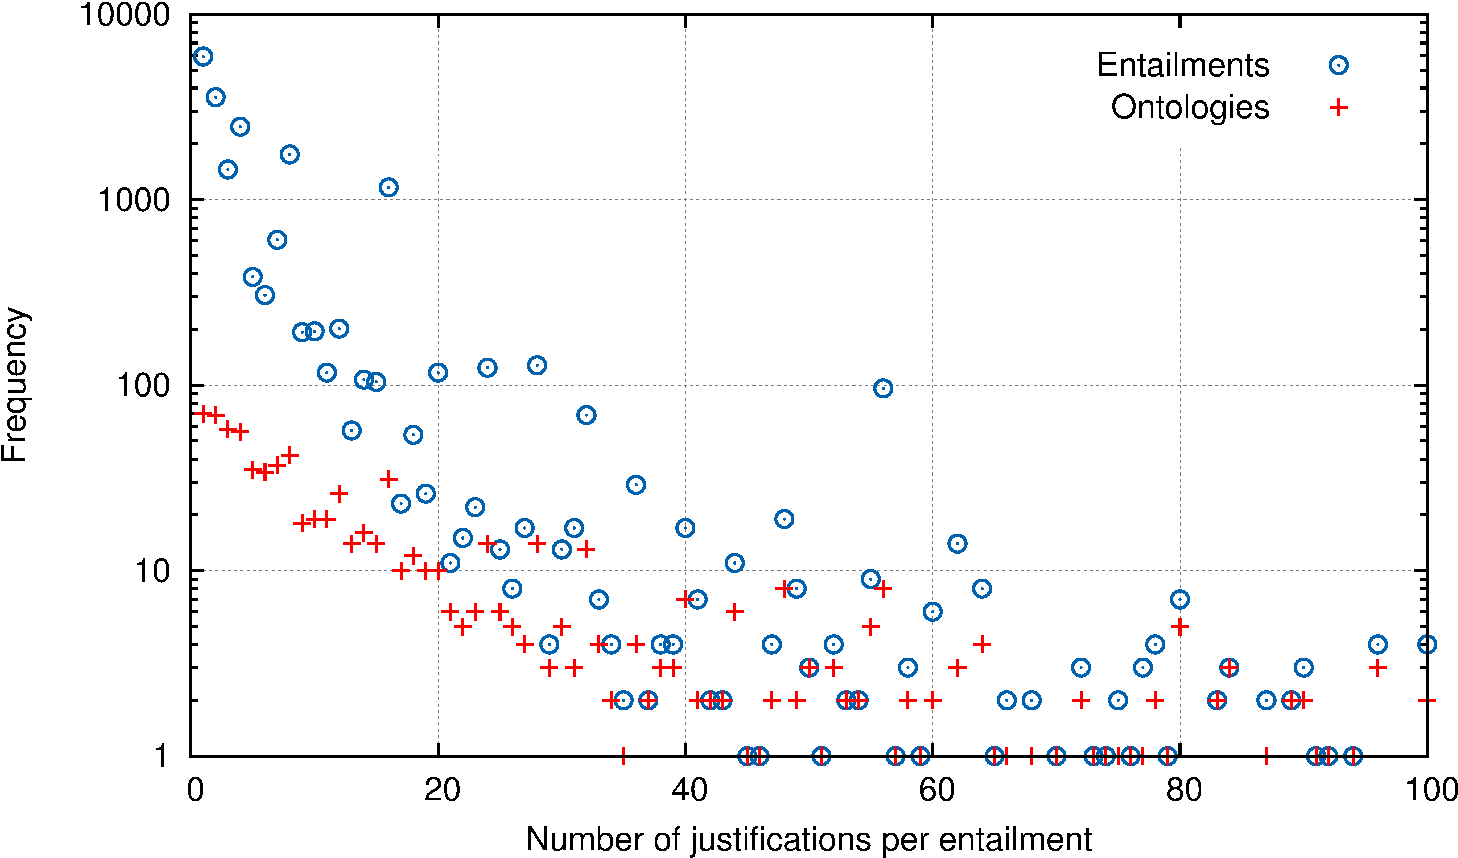
\includegraphics[width=14cm]{plots/frequency.pdf}
\caption{Frequency of multiple complex justifications in the corpus.}
\label{fig:frequency-justperent-nonself-sat}
\end{figure}

In $S_{u}$, the average number of justifications per entailment is 24.1 (\sdev = 12.8, \median = 32), with a maximum of 55 justifications for entailments in the \emph{Quantitative Imaging Biomarker} ontology. 7 of the 10 ontologies contain only entailments with exactly 1 justification, whereas the remaining 3 ontologies contain only entailments with multiple justifications. 

While we might expect to see a correlation between the size of an ontology and the number of complex justification it generates, we found that there are no obvious indicators for the occurrence of multiple justifications in an ontology. The Spearman rank coefficient\footnote{A coefficient $\rho$ of +1 (-1) indicates a strong positive (negative) correlation between two variables, whereas a $\rho$ of 0 indicates no correlation.} $\rho = 0.09$ ($p = 0.43$) indicates no correlation between the number of logical axioms in an ontology in set $S_{s}$ and the number of justifications per entailment. Due to the small number of ontologies in $S_{u}$, the correlation analysis was only performed for $S_{s}$.

\paragraph{Ontology activity and axiom power}

The 145,689 complex justifications in $S_{s}$ contain a total of 22,371 axioms. On average, one fifth of the axioms in an ontology (22.2\%, \sdev = 20.4\%, \median = 15.1\%) are active in  complex justifications for their entailed atomic subsumptions, with some ontologies having as many as 75.5\% of their axioms participating in justifications. Note that the small number of axioms compared to the number of justifications indicates a high amount of shared axioms in the corpus; we will focus on the matter of axiom overlap below.

Intuitively, we would expect to see an obvious correlation between the number of entailments in an ontology and its activity (the proportion of active axioms), since more entailments would imply more justifications and axioms occurring in them; this is somewhat confirmed by $\rho = 0.49$ (Pearson's correlation coefficient) indicating a weak linear correlation ($p < 0.001$).


\paragraph{Graph components}
In order to determine the overall connectedness of justifications, we consider the number of connected components in each j-graph. On average, each graph contains 4.6 (\sdev=9.8, \median=2) connected components, but almost half of the graphs in $S_s$ (37 out of 78) consist of exactly one component. The largest number of components can be found in the \emph{International Classification for Nursing Practice} ontology, which has 1,063 complex justifications for 762 entailments that are split up over 68 components.

As we have mentioned in previous chapters, the justification finding algorithm uses the Hitting Set Tree algorithm, which depends on optimisations such as justification reuse. This implies that largely disjoint justification sets may have a negative impact on the performance of the \enquote{find all} algorithm. However, there seems to be no correlation between the number of components in a j-graph and the average time required to find a justification ($\rho$ = 0.13, $p = 0.25$), or the number of components and the number of calls to the \enquote{find one} subroutine ($\rho$ = 0.06, $p = 0.58$).\footnote{Note, however, the high p-values which indicate that these findings are not statistically significant.}


\subsection{Justification overlap}

\paragraph{Inferential power of justifications}

While multiple justifications per entailment occur very frequently in the corpus, the number of justifications with multiple entailments is comparatively low, with only 709 justifications in $S_{s}$ having out-degrees $\geq2$ in the j-graph. On average, a justification in $S_{s}$ has 1.1 entailments (\sdev = 2.2, \median = 1), with a maximum of 120 entailments for 16 fairly small justifications (containing 5 to 7 axioms) in the \emph{SNP} ontology. Across the corpus, only 17 out of the 78 ontologies contain justifications with multiple entailments.

There is no correlation between the size of a justification and its number of entailments ($\rho$ = -0.07, $p < 0.001$). The average size of justifications that have only one entailment is 7.9, with some of the largest justifications (20 and more axioms) having only one entailment, whereas the average size of a justification with multiple entailments is 4.2 axioms.


\paragraph{Axiom frequency and impact}

Regarding the frequency and impact of the axioms in the corpus, we want to find out how frequently axioms occur in multiple justifications, and how many entailments these axioms affect. On average, an axiom occurs in 51.3 justifications (\sdev = 242.1, \median = 5) in set $S_{s}$, with some key axioms in several ontologies occurring in thousands of justifications. Figure \ref{fig:arityimpact} shows the axiom frequency plotted against the average impact, following approximately a linear distribution as shown by the linear trendline.\footnote{Again, the \enquote{long tail} of the plot of up to 7,343 justifications has been cut off for presentation purposes.} 

\begin{figure}[tb]
\centering
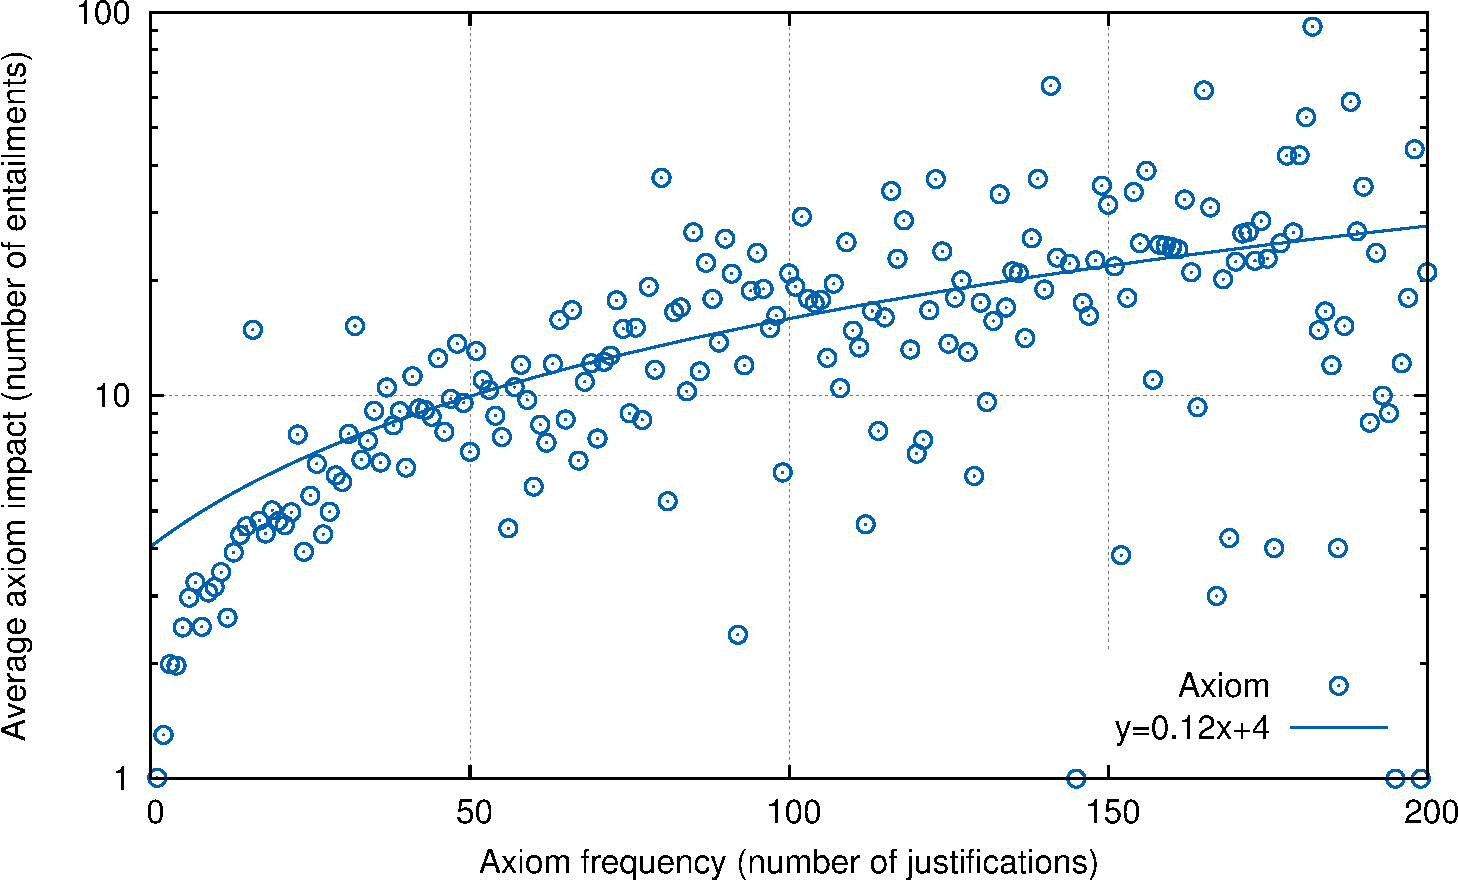
\includegraphics[width=14cm]{plots/arityimpact.pdf}
\caption[Axiom frequency vs average axiom impact.]{Axiom frequency vs average axiom impact, fitted with a linear trendline.}
\label{fig:arityimpact}
\end{figure}

The closeness of axiom frequency and impact is not surprising, since we have already seen that most justifications in the corpus only have a single entailment; therefore, the impact for most axioms is less than (if they occur in justifications for the same entailment) or equal to (if they occur in justifications for different entailments) the number of justifications they occur in. 

Interestingly, all the ontologies in the corpus (even those which contain only small numbers of justifications) contain some axiom which occurs in multiple justifications, and 23 ontologies contain some axiom which occurs in over 50\% of the justifications in the ontology. On average, the one axiom with the highest frequency in an ontology occurs in 36.3\% of all justifications of an ontology. 

An example of such a high-frequency axiom is the simple atomic subsumption \ax{Disease \subcls Disposition} which is used in 3,119 (96.5\%) of the 3,232 justifications in the \emph{NIF Dysfunction} ontology and affects 423 entailments. Another example is the domain axiom \ax{domain(measuredBy, MentalConcept)} in the \emph{Cognitive Atlas} ontology, which occurs in 92.5\% of the 830 justifications for 126 entailments.



\paragraph{Root and derived justifications}
Root and derived relationships occur frequently across the corpus: 73.4\% of the justifications in $S_{s}$ are derived, and 7.4\% of the justifications are root justifications which have derived justifications. The remaining 19.2\% are root justifications that do not have any justifications that are derived from them, that is, they are either additional independent justifications for derived entailments, or justifications for entirely independent root entailments. Table \ref{tab:rootderived} gives an overview of the root and derived relationships in the corpus; root justifications that are subsets of derived justifications are denoted by $Justs_{rsub}$, root justifications that are no subsets are denoted by $Justs_{r}$, and derived justifications are denoted by $Justs_{d}$.

\begin{table}
\centering
\caption[Root and derived justifications in $S_{s}$ and $S_{u}$.]{Root and derived justifications in $S_{s}$ and $S_{u}$, in number of justifications and proportion of the total.}
\label{tab:rootderived}	
\begin{tabu}{lrrrrrrr}
\toprule
&  & \multicolumn{2}{c}{$Justs_{rsub}$} & \multicolumn{2}{c}{$Justs_{d}$} & \multicolumn{2}{c}{$Justs_{r}$}\\
\cmidrule(r){3-4} \cmidrule(r){5-6} \cmidrule(r){7-8}
Set		& Total & Count & \% & Count & \% & Count & \% \\
\midrule
$S_{s}$ & 145,689 & 10,723 & 7.4\% & 107,002 & 73.4\% & 27,964 & 19.2\% \\
$S_{u}$ & 10,352 & 115 & 1.1\%  & 10,184 & 98.4\% & 53 & 0.5\% \\
\bottomrule 
\end{tabu} 
\end{table}

Looking at the repair impact of root justifications, we find that a justification in $Justs_{rsub}$ has 17 justifications on average which are derived from it (\sdev = 92.8, \median = 3), and 5.4 entailments (\sdev = 19.5, \median = 2) that are entailed by these derived justifications. In other words, while a root justification may have a fairly large number of justifications (17) that are derived from it, the number of entailments that can be repaired by fixing a single root justification is comparatively low (5.4).

The subset relationship between root and derived justifications is also visible in the size of justifications: on average, a root justification contains 4.7 axioms, whereas a derived justification has a size of 8.4 axioms. 7.6\% of the root justifications are indeed single axiom justifications which occur in a large number of derived justifications. However, while we may expect a small justification to be more likely to be contained in derived justifications, there is only a weak correlation between the size of a root justification and the number of justifications that are derived from it ($\rho = -0.26, p < 0.001$).

70 of the 78 ontologies in $S_{s}$ contain some derived justifications. 6 of of the 8 remaining ontologies only contain very small numbers of justifications, which do not lend themselves to subset relationships, whereas the \emph{Cancer Research and Management} ontology and \emph{Gene Ontology Extension} contain no derived justifications despite having 348 and 6,421 justifications, respectively.

In the set $S_{u}$, the effect of root and derived justifications is even more pronounced: 98.4\% of the justifications are derived from only 1.1\% of the justifications, and the remaining 0.5\% are root justifications which have no derived justifications. On average, a root justification has 88.6 derived justifications (\sdev = 208.6, \median = 2) which have 48.8 entailments (\sdev = 109.3, \median = 2). Note how this stands in contrast to the rather small number of entailments (5.4) that depend on root justifications in $S_{s}$. 5 of the 10 ontologies in $S_{u}$ contain root and derived unsatisfiable classes, whereas the remaining 5 ontologies contain only very few unsatisfiable classes (up to 4) at all.


\paragraph{Arbitrary overlap}

In order to determine the numbers and sizes of justification overlaps with more than a single axiom, we applied the Formal Concept Analysis (FCA) \cite{ganter05ar} \enquote{next concept} algorithm to the j-graphs in sets $S_{s}$ and $S_{u}$. This algorithm (often simply referred to as \enquote{Ganter's algorithm}) provides an efficient means for computing the largest shared axiom sets between justifications. The ToscanaJ FCA framework\footnote{\url{http://toscanaj.sourceforge.net/}} includes a straight-forward implementation of Ganter's algorithm, which we used for overlap detection. Using the FCA algorithm, the justifications correspond to the \emph{objects} in a  context, and the axioms correspond to the \emph{attributes}. Due to performance issues, the experiment was restricted to a random sample of maximum 5,000 edges per graph. 

\begin{figure}
\centering
		\begin{subfigure}{0.5\textwidth}
                \centering
                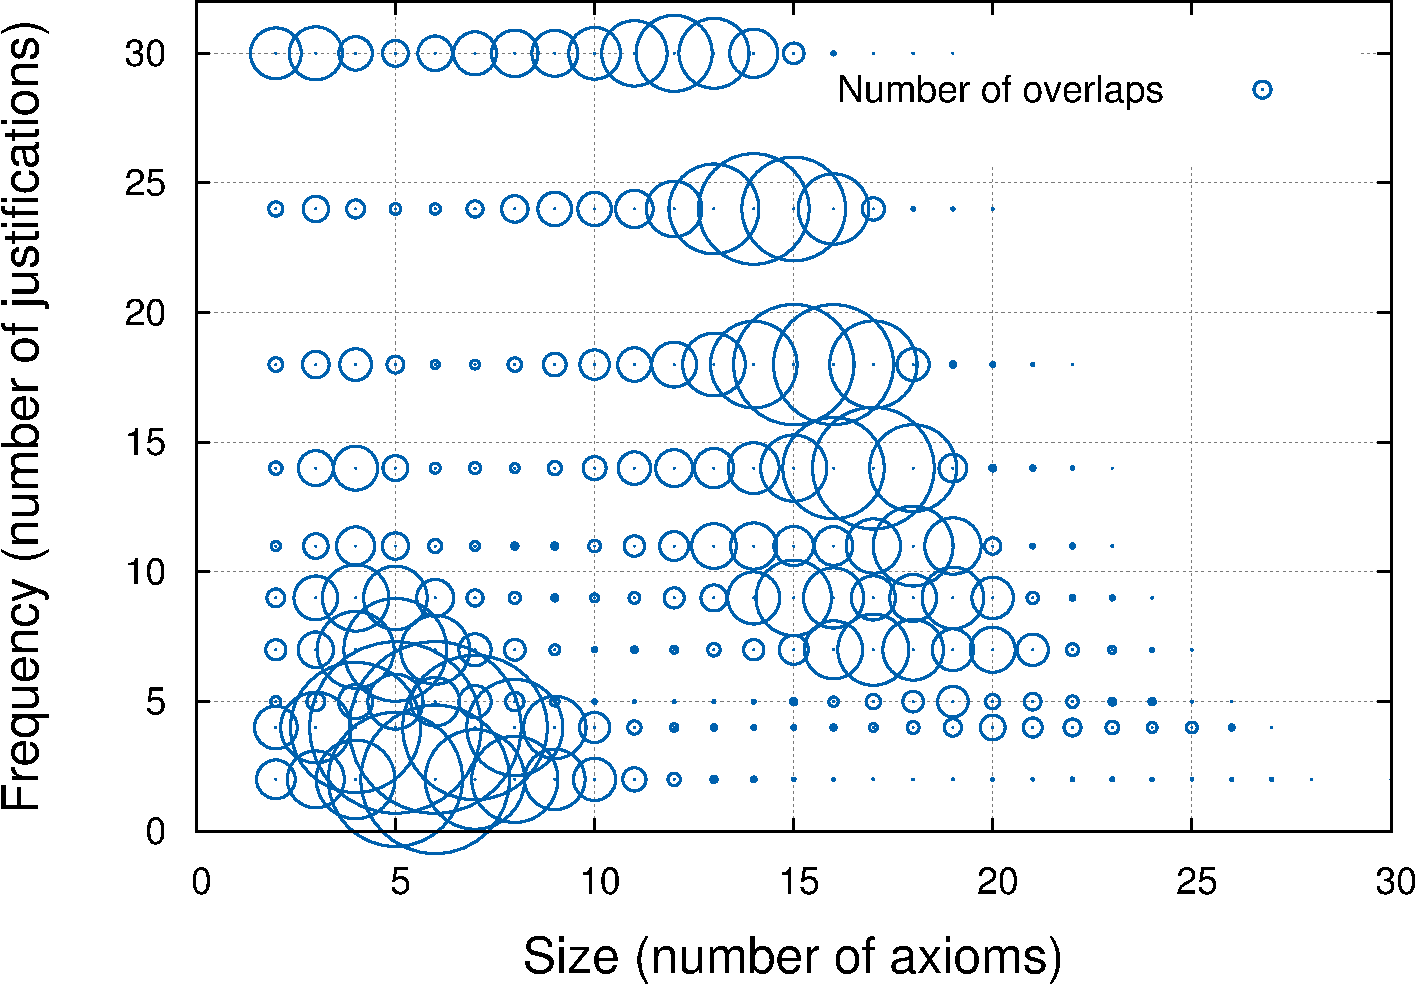
\includegraphics[height=5.2cm]{plots/overlap-count-all.pdf}
                \caption{Overlap frequency for \textbf{all} ontologies \\in $S_{s}$.}
        	\label{fig:overlap-all}
        \end{subfigure}%
         %add desired spacing between images, e. g. ~, \quad, \qquad etc. 
          %(or a blank line to force the subfigure onto a new line)
		\begin{subfigure}{0.5\textwidth}
                \centering
                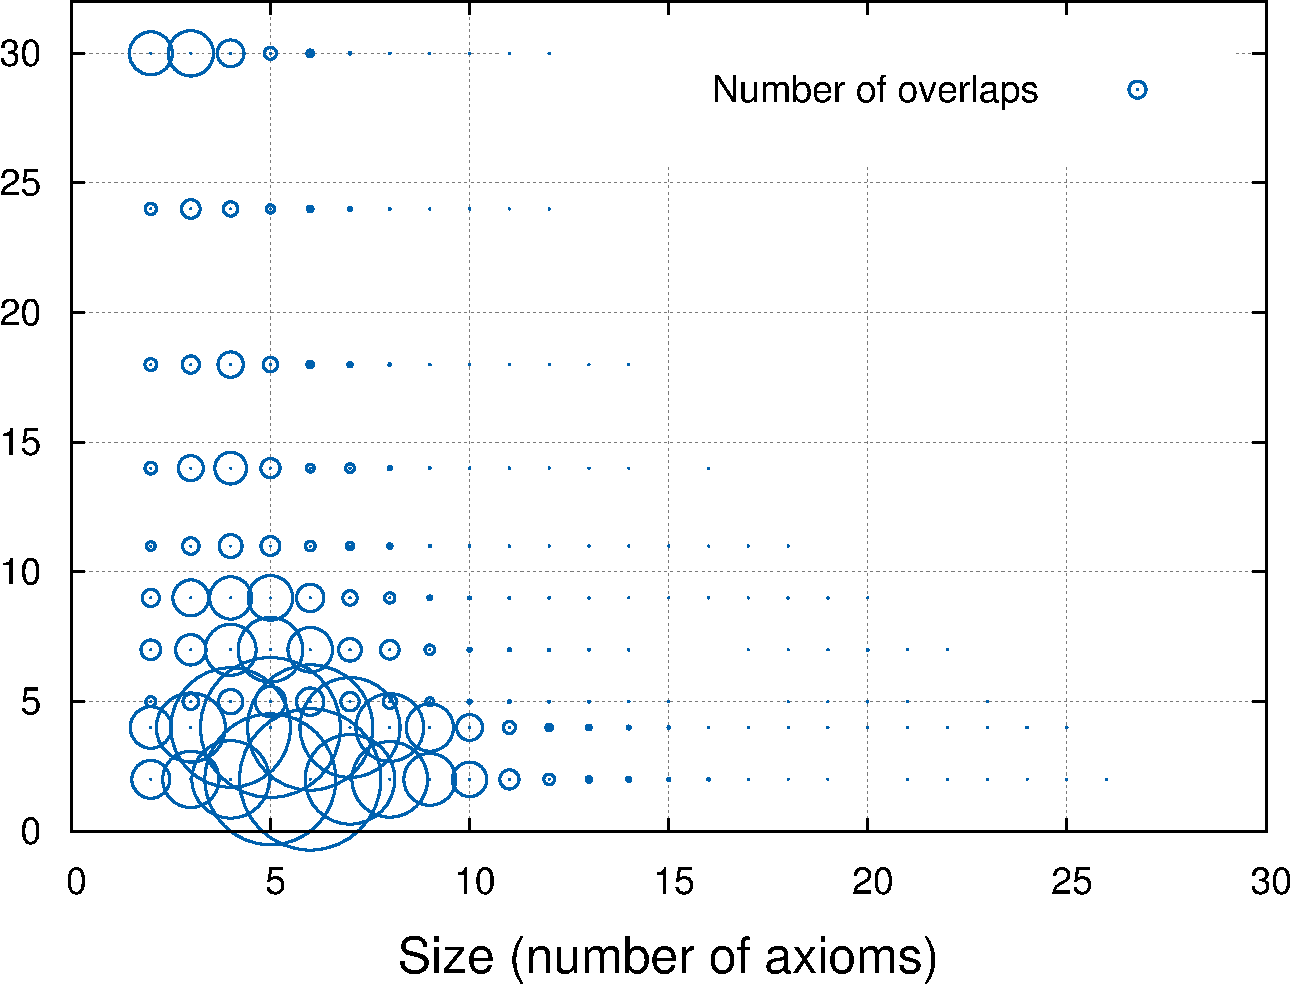
\includegraphics[height=5.2cm]{plots/overlap-count-reduced.pdf}
                \caption{Overlap frequency \textbf{excluding} \emph{Amino Acid} and \emph{Basic Vertebrate Anatomy}.}
        	\label{fig:overlap-reduced}
        \end{subfigure}
        \caption[Overlap frequency with and without outlier ontologies.]{Overlap frequency with and without outlier ontologies. Bubble size indicates frequency.}
\end{figure}

Across the ontologies in $S_{s}$, overlaps between justifications occur frequently, with an average size of 10.8 shared axioms (\sdev = 5.7, \median = 11) and an average frequency of 11.9 justifications (\sdev = 11.8, \median = 9) that the shared axiom set occurs in, i.e.\ on average, 11.9 justifications share the same axiom set. Figures \ref{fig:overlap-all} and \ref{fig:overlap-reduced} show the frequency of overlap of different size and frequency across the corpus including and excluding the two ontologies which contribute the largest numbers of overlaps. For presentation purposes, the values on the y-axis (i.e.\ the number of justification an overlap of a certain size occurs in) were binned in 10th percentile steps, leading to all overlaps with a frequency greater than 24 falling into the top-most bin. 

The plot shows that the majority of overlaps (i.e.\ the largest bubbles) have a size of around 5 axioms and occur in up to 5 justifications. However, there are also overlapping cores of around 15 to 20 axioms which occur fairly frequently in up to 18 justifications; as we can see if we compare \ref{fig:overlap-all} to \ref{fig:overlap-reduced}, these large, high-frequency overlaps are almost exclusively contributed by the \emph{Amino Acid} and \emph{Basic Vertebrate Anatomy} ontologies. If we exclude these two ontologies from the set, the overlaps are reduced to an average of 5.5 axioms (\sdev = 2.5, \median = 5) and a frequency of 7.8 justifications (\sdev = 14.3, \median = 4).

Nearly all ontologies in $S_{s}$ (75 out of 78) contain at least some overlapping justification subset, with two ontologies standing out as extreme outliers.  The \emph{Amino Acid} ontology contributes over half of the found overlaps in the corpus, which is rather surprising, as with 112 entailments, 477 axioms, and a description logic expressivity of \dl{ALCF}, this ontology could be considered fairly inexpressive.

However, if we take a closer look at the \emph{Amino Acid} ontology, we find that it contains an axiom of the type \ax{AminoAcid \eqcls A \disj C \disj D \ldots \disj Y} with 20 named classes in the disjunction. This axiom, in turn, leads to a large number of justifications (2,652) containing subsumption axioms for each operand in the disjunction, plus a small number of \enquote{bridging} axioms that cause the entailment to hold. For 1,782 of the 2,562 justifications, this axiom pulls in a large core of up to 29 other axioms, thus leading to the large numbers of overlaps observed in the ontology.

A similar effect can be seen in the \emph{Basic Vertebrate Anatomy} ontology, another fairly small ontology (99 classes, 386 axioms, \dl{SHIF}) which, however, has a high number of object properties (74 compared an average of 22.2). The ontology contains a number of axioms describing the relations between its object properties as part-whole relationships, such as \ax{has\_subdivision \subcls has\_determinate\_part} and \ax{is\_subdivision\_of \eqcls \inv{has\_subdivision}}. Again, these property axioms pull in other \enquote{bridging} axioms which leads to cores of up to 17 axioms occurring in large numbers of justifications.

Both of these outlier ontologies have high degrees of overlaps between multiple justifications for \emph{single} entailments, but only small numbers of overlaps between justifications for several different entailments. This agrees with the general trend in the corpus, where on average those  justifications which do share an overlap only have between 1 and 2 entailments (mean = 1.9, \median = 1, \sdev = 5.1). In other words, overlap tends to occur mainly between justifications for the \emph{same} entailment.


\subsection{Justification isomorphism}

In order to determine the frequency of isomorphic justifications in the corpus, we analysed the complex justifications for the entailments in set $S_{s}$ and $S_{u}$ in three different experiments: 
\begin{compactenum}
\item justifications for a \emph{single} entailment.
\item justifications for \emph{all} entailments within an ontology.
\item justifications for \emph{all} entailments of all ontologies across the corpus.
\end{compactenum}
The isomorphism statistics were generated for all three types of isomorphism, that is, strict, subexpression-, and lemma-isomorphism. 

Due to performance issues, justifications containing more than 10 axioms or conjunctions/disjunctions with more than 5 operands were excluded from this part of the study. This excluded some dominant justifications (such as those containing the large disjunction axiom in the \emph{Amino Acid} ontology mentioned above), but still resulted in a set of 141,560 justifications for 19,097 entailments in $S_{s}$, which is an average of 7.4 justifications per entailment (compared to 7.8). Note that this also means that the total numbers of justifications given in this section for some of the ontologies will differ from the number of complex justifications listed in the overview table in Appendix A.

The mean times required to determine isomorphism between justifications for each of the three types (including parsing the justifications and existing templates from file) are listed in Table \ref{tab:iso-times}. Note that the experiments for the three isomorphism types were run in parallel, which could potentially cause a drop or fluctuations in performance (as the \enquote{Within ontology} times for strict versus subexpression-isomorphism show). Furthermore, the checks within ontologies and across the corpus each reuse the templates found in the previous stage, which drastically reduces the number of comparisons that have to be carried out. 

\begin{table}[htb]
\centering
\caption{Mean times (in seconds) per ontology for isomorphism detection.}
\label{tab:iso-times}	
\begin{tabu}{lrrrrrr}
\toprule
 Size & Iso  & S-iso & L-iso\\
\midrule
Individual entailments 	&	22.8	&  48.5	& 100.8  \\
Within ontology 		&	103.8	&  99.2	& 192.3  \\
Across corpus 			&	24.6	&  42.3 &  97.7 \\
\bottomrule 
\end{tabu} 
\end{table}


\subsubsection{Individual entailments}

\paragraph{Strict isomorphism}
Due to restrictions on the types of justifications used in the isomorphism experiments, the number of justifications for the entailments in this subset of $S_{s}$ is marginally lower than in the j-graph analysis, with an average of 7.4 justifications per entailment. Strict isomorphism reduces this number to an average of 4.9 templates per entailment (\sdev = 9.5, \median = 2), which is a reduction by 33.7\% compared to the full corpus.

On average, a template covers 1.5 justifications (\sdev = 2.3, \median = 1), with some ontologies containing entailments with large numbers of isomorphic justifications. One such example is the \emph{Orphanet Ontology of Rare Diseases}, whose dominating templates are of the type
\begin{align*}
\Theta_{1} =\{\dlax{C1 \subcls C2}, \dlax{C2 \subcls \exists p1.C4}, \dlax{domain(p1, C3)} \} \models \dlax{C1 \subcls C3}
\end{align*}
with atomic subsumption chains of arbitrary size in place of the first subsumption axiom, and some variations that include subproperty axioms. Two of the templates of this type cover the majority (110 and 105 justifications, respectively) of the 220 justifications each for several entailments in the ontology. From personal contact with the \emph{Orphanet} developers we have learned that this OWL ontology is in fact generated automatically from an existing medical database, which explains the frequent occurrences of uniform justifications.


\paragraph{Subexpression-isomorphism}

Subexpression-isomorphism across the justifications of individual entailments only affects a very  small number of entailments in the corpus. The average number of templates per entailment, compared to the full corpus, remains the same when rounded,\footnote{The precise number of templates is 4.915 for strict and 4.903 for subexpression-isomorphism.} at 4.9 templates per entailment (\sdev = 9.5, \median = 2). Compared to strict isomorphism, the number of templates is reduced by only 0.3\%. This small reduction does not affect the average number of justifications per entailment, which remains the same at 1.5 justifications.

Only 166 entailments (0.9\% of the total corpus) from 15 of the 78 ontologies are affected by subexpression-isomorphism; the remaining 63 ontologies contain the same number of templates as for strict isomorphism. For those ontologies that are affected, the decrease in templates compared to strict isomorphism is an average of 19.8\%, reaching up to 50\% for 9 entailments in the \emph{Bleeding History Phenotype} ontology.

\paragraph{Lemma-isomorphism}

While subexpression-isomorphism does not have a strong effect on individual entailments, lemma-isomorphism shows a more visible reduction in template numbers.\footnote{Note that $S_{s}$ and $S_{u}$ do not contain any justifications that consist entirely of atomic subsumption chains. That is, all atomic subsumption chains that are affected by l-isomorphism will be strict subsets of the complex justifications in the corpus.} On average, the justifications are reduced to 4.7 templates per entailment (\sdev = 8.8, \median = 2), which is reduction by 4.1\% compared to both strict and subexpression-isomorphism.

A total of 1,492 entailments (7.8\% of the total corpus) from 43 ontologies are affected by lemma-isomorphism, with an average reduction of 30.3\% compared to strict isomorphism for those entailments. The strongest effects can be seen in the \emph{Fission Yeast Phenotype} ontology, where the justifications for several entailments only differ in the length of their atomic subsumption chains and thus are each reduced to a single template of the type \begin{align*}
\Theta_{2} = \{\dlax{C1 \subcls \ldots \subcls C_{n}, C_{n} \eqcls C2 \conj \ldots} \} \models \dlax{C1 \subcls C2}.
\end{align*}


\subsubsection{Isomorphism within ontologies}

Across the justifications for all entailments of an ontology, the reductions caused by the three equivalence relations are more clearly visible than for individual entailments. Figure \ref{fig:iso-comparison} shows an overview of the effects of the different isomorphism types for the 25 ontologies containing the largest numbers of justifications in the corpus. Each cluster represents an ontology, with the ontologies ordered by the number of justifications they contain. Each bar in a cluster represents the reduction compared to the previous equivalence relation (that is, we compare strict isomorphism with the full set of justifications, s-isomorphism with strict isomorphism, and l-isomorphism with s-isomorphism). We can see that the effects of the relations differ strongly across the ontologies, with strict isomorphism generally having the strongest impact, and subexpression-isomorphism having the lowest impact.

Overall, only three ontologies show no effect for \emph{any} of the three types of isomorphism; two of these contain only a single justification (which means there is no reduction possible), while one ontology (\emph{OBOE SBC}) contains 5 distinct justifications.


\begin{figure}
\centering
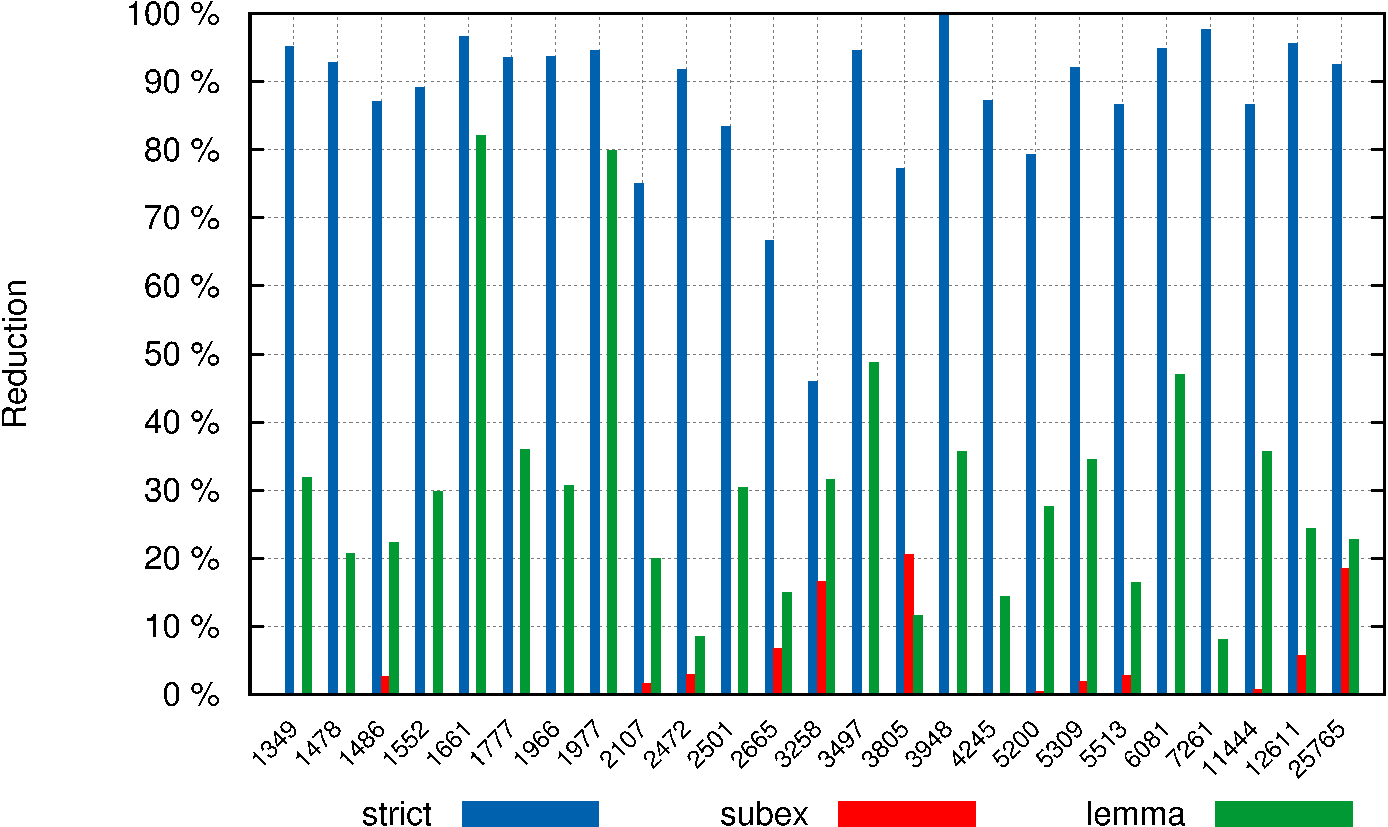
\includegraphics[width=14cm]{plots/iso-comparison.pdf}
\caption[Comparison of reduction caused by isomorphism types.]{Comparison of reduction caused by isomorphism types. Each cluster represents an ontology. Ontologies are ordered by number of justifications.}
\label{fig:iso-comparison}
\end{figure}


\paragraph{Strict isomorphism}

Compared to the results for individual entailments, the effects of the equivalence relations are much more significant if we consider the justifications for \emph{all} entailments in an ontology. On average, an ontology in $S_{s}$ contains 1,814.9 justifications; these are reduced to 436.1 templates through strict isomorphism, which is an average reduction by 73.1\%.

4 ontologies with small numbers of justifications (less than 10) are not affected by strict isomorphism, while the remaining 74 ontologies show reductions of up to 99.6\%. Even more strikingly, 28 of the ontologies are reduced to less than 10\% of their justification corpus. With an average number of 3,092 justifications per ontology, these reductions reveal significant numbers of structurally similar justifications.

The templates cover an average of 8.2 justifications each (\sdev = 22.4, \median = 2), with some of the highest coverage occurring in the \emph{Orphanet} ontology. The 3,948 justifications in this ontology can be reduced to only 14 templates, which are all variations (featuring atomic subsumption chains of varying length) of the template $\Theta_{2}$ we have shown above.


\paragraph{Subexpression-Isomorphism}

Subexpression-isomorphism reduces the justifications in the corpus by an average of 74\% per ontology, which is only a small change (0.9\%) compared to strict isomorphism. The number of justifications covered by a single template is slightly increased to 8.8 (\sdev = 23.5, \median = 2) justifications per template.

Again, the majority of ontologies (44 of 78) are not affected by subexpression-isomorphism, whereas 5 ontologies show reductions of between 20\% and 38.3\% compared to strict isomorphism. This includes the \emph{Bleeding History Phenotype} ontology (1,158 justifications, 60 isomorphism templates, 37 s-isomorphism templates), which contains a number of justifications of the type
\begin{align*}
\{ \dlax{C1 \subcls \exists p1.(C2 \disj C3)}, \dlax{domain(p1, C4)} \} \models \dlax{C1 \subcls C4}
\end{align*}
which is subexpression-isomorphic to justifications which contain a named class in place of the disjunction $C2 \disj C3$ in the subsumption axiom, thus matching template $\Theta_{1}$.

Closer inspection of the \emph{Lipid} ontology (3,258 justifications as shown in Figure \ref{fig:iso-comparison}, 1,762 isomorphism templates, 1,471 s-isomorphism templates) reveals that a large number of justifications in the ontology consist of a single equivalence axiom of the form \dlax{C1 \subcls C2 \conj x} with the entailment being \dlax{C1 \subcls C2}. The remainder of the conjunction, represented by $x$, consists of a number of complex expressions of varying length and nesting depth. While s-isomorphism captures these types of justifications (since the remainders $x$ can all be matched against each other), the actual reason for their similarity lies in their identical \emph{cores} \dlax{C1 \subcls C2}, with the remainder $x$ being a superfluous part.

\paragraph{Lemma-isomorphism}

As for single entailments, lemma-isomorphism has a more significant effect on the justification corpus than subexpression-isomorphism when applied across each ontology. L-isomorphism reduces the justifications in an ontology by an average of 78.2\%, which is a 4.2\% difference compared to subexpression-isomorphism. 

A template covers an average of 12 justifications (\sdev = 38, \median = 3) in each ontology, which is a visible increase from the 8.8 justifications covered by subexpression-isomorphism. 13 ontologies (with an average number of 32.1 justifications) show no reaction to l-isomorphism, whereas 12 ontologies containing large numbers of justifications (mean = 1,555.8) see a reduction of 41.7\% and more, up to 82.1\% compared to subexpression-isomorphism.

\subsubsection{Isomorphism across the corpus}

In the final stage of our analysis of isomorphism in the BioPortal corpus, we will look at the templates spanning all justifications for all entailments across the ontologies in the corpus. While we have seen that isomorphic justifications occur frequently within an ontology, we now analyse the structural similarity of justifications across multiple ontologies. Table \ref{tab:iso-cross} gives an overview of the numbers of templates in $S_{s}$ for the three isomorphism types against the full justification corpus, as well as the coverage (number of justifications) per template.

\begin{table}
\centering
\caption{Template frequency and coverage across the corpus.}
\label{tab:iso-cross}
\begin{tabu}{lrrrrrr}
\toprule 
		& 			& 		&  \multicolumn{4}{c}{Coverage} \\
\cmidrule(r){4-7}
Type & Count & \% of $S_{s}$ &  Mean & Median & Min & Max \\
\midrule 
all 	& 141,560 	& 100\% 	& - 		&  - 	& - & - \\
strict 	& 12,527 	& 8.8\%  	& 11.3  	&  2 	& 1 & 2,072 \\
subex 	& 10,952 	& 7.8\%  	& 12.9 		&  2	& 1 & 2,128  \\
lemma 	& 5,487  	& 3.1\%    & 25.8 		& 3 	& 1 & 7,490      \\
\bottomrule 
\end{tabu} 
\end{table}

\paragraph{Strict isomorphism}

The 141,560 justifications in $S_{s}$ are reduced to only 12,527 templates, which is a reduction by 91.2\%. On average, 11.3 justifications (\sdev = 54.3, \median = 2) share the same template, with the 8 most frequent templates covering over 1,000 justifications each. The most frequent templates (by numbers of justifications covered) are all variations of the template $\Theta_{1}$, that is, a combination of a domain axiom and a subsumption axiom with an existential restriction on the RHS, including some additional subsumption axioms, an equivalence axiom in place of a subsumption, or variations of the filler.

Nearly half of all templates (41.3\%) in the corpus cover exactly one justification in a single ontology. We might larger templates to be more \enquote{specific} to a particular ontology, thus covering fewer justifications overall, and conversely, a smaller template might be more \enquote{generic}, thus covering more justifications. However, the size (number of axioms) of a template seems to be no indicator for the number of justifications it covers: the average size (7.3 axioms) of a template covering multiple justifications is only marginally lower than of those templates covering a single justification (7.5 axioms). 

If we look at the spread of templates across the ontologies in the corpus, we find that only 8.7\% of the templates cover justifications in multiple ontologies, with a maximum spread of 26 ontologies for two templates which are, again, variations of $\Theta_{1}$. Figure \ref{fig:iso-freq} shows the frequency distributions of the justification templates across the justifications and ontologies in $S_{s}$. The y-position of a data point indicates the number of justifications a template covers is, and the bubble size indicates the number of ontologies a template occurs in. 

We can see that a small number of templates covers large numbers of justifications, with a steep drop to 10 and less justifications per template around the 2,000 mark. If we take a closer look at the numbers, we find that the majority of justifications in the corpus (81.2\%) are covered by the 2,000 most frequent templates (out of 12,527), and a third (33.1\%) of justifications are even covered by the 100 most frequent templates.

\begin{figure}
\centering
		\begin{subfigure}{0.5\textwidth}
                \centering
                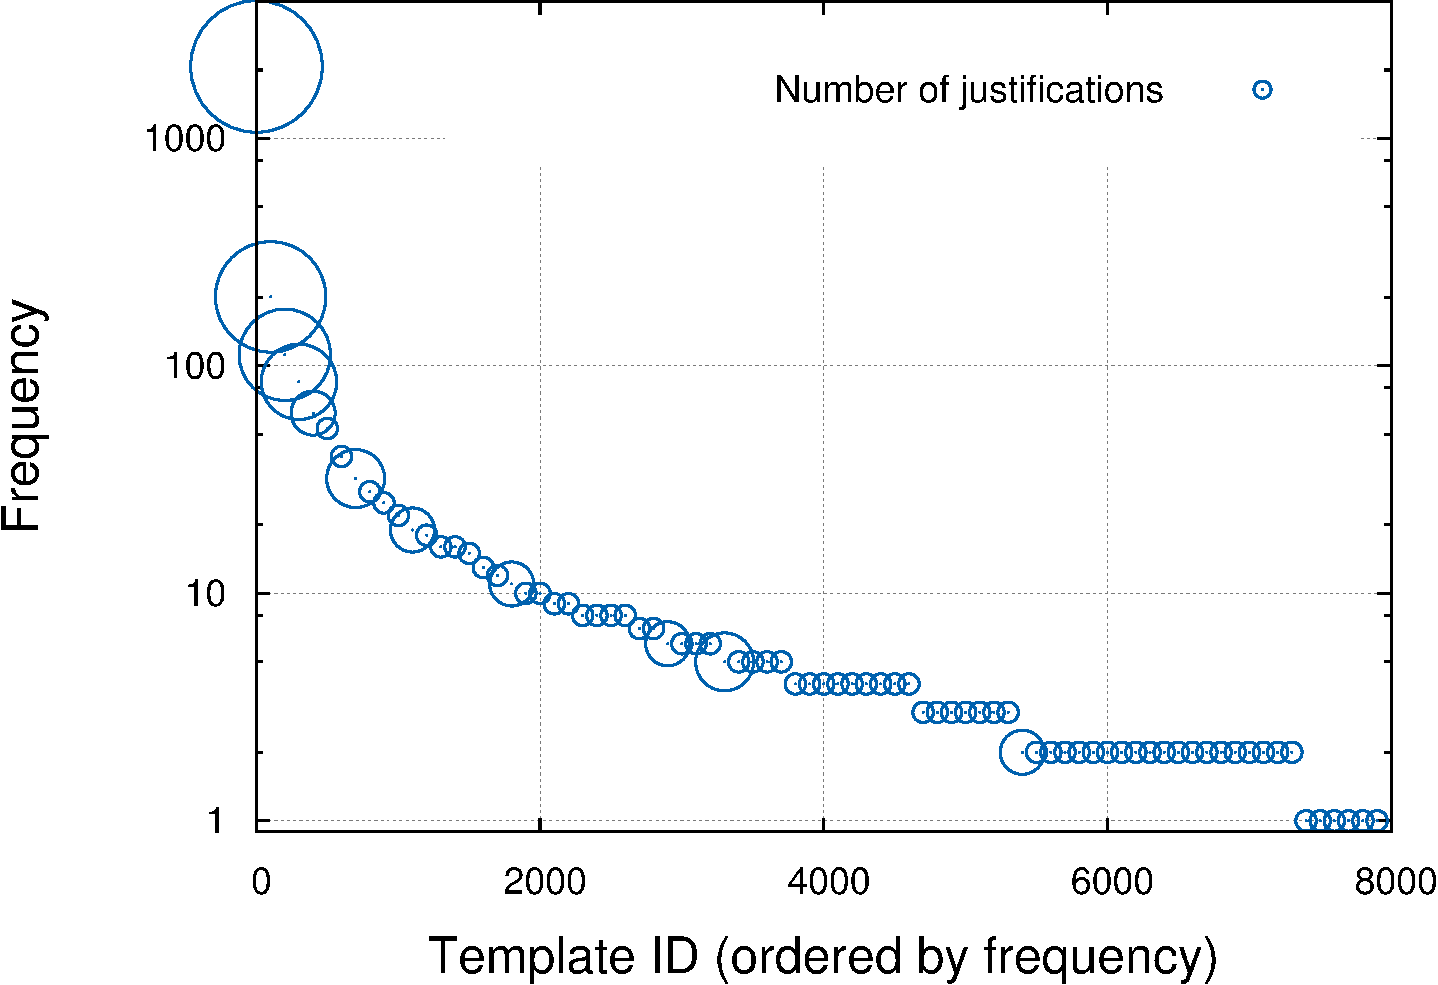
\includegraphics[height=5.2cm]{plots/iso-template-freq.pdf}
                \caption{Template frequency for strict iso.}
        	\label{fig:iso-freq}
        \end{subfigure}%
         %add desired spacing between images, e. g. ~, \quad, \qquad etc. 
          %(or a blank line to force the subfigure onto a new line)
		\begin{subfigure}{0.5\textwidth}
                \centering
                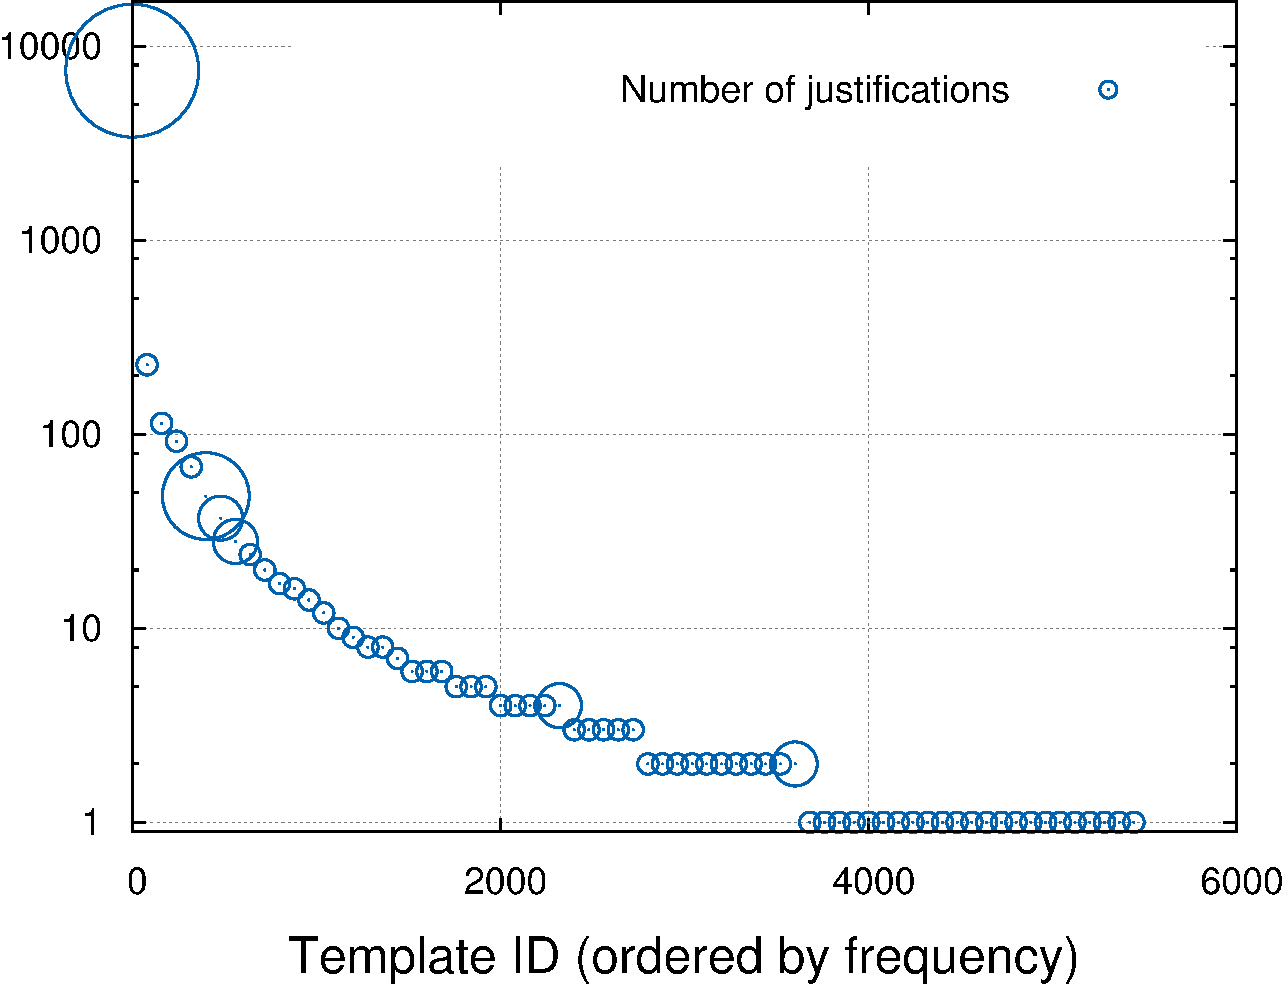
\includegraphics[height=5.2cm]{plots/iso-template-freq-lemma.pdf}
                \caption{Template frequency for l-iso.}
        	\label{fig:iso-freq-lemma}
        \end{subfigure}
        \caption{Template frequencies for strict and lemma-isomorphism.}
\end{figure}

\paragraph{Subexpression-isomorphism}
The effects of subexpression-isomorphism across the corpus are only marginal compared to strict isomorphism. The justifications are reduced to 10,952 templates, which is an overall reduction by 92.2\% and a 1\% difference compared to strict isomorphism. The number of justifications covered by a single template is slightly increased with an average of 12.9 justifications (\sdev = 59, \median = 2) per template.

The most frequent template (by numbers of justifications) is again $\Theta_{2}$, which covers 2,128 (1.5\% of the total set) justifications in 26 ontologies. Across the ontologies in the corpus, the most frequent template occurs in 28 of the 78 ontologies. This template is a single equivalence axiom which we have already seen in the \emph{Lipid} ontology:
\begin{align*}
\Theta_{3} = \{\dlax{C1 \eqcls C2 \conj x} \} \models \dlax{C1 \subcls C2}
\end{align*}
The superfluous part $x$ matches a number of operands such as atomic classes and existential restrictions. Interestingly, while this template occurs in the highest number of ontologies, it only covers 573 justifications across the corpus.


\paragraph{Lemma-isomorphism}

Across all justifications in the corpus, l-isomorphism has a clearly visible impact. The 141,560 justifications are reduced to only 5,487 templates, which is less than half as many templates as the strictly isomorphic ones, and an overall reduction of 96.9\%. Figure \ref{fig:iso-freq-lemma} shows the frequency of templates for lemma-isomorphism.

On average, a template covers 25.8 justifications (\sdev = 208.5, \median=3); however, the large standard deviation shows that the distribution of justifications per template has shifted towards a few very frequent templates, whereas there is still a \enquote{long tail} of 1,878 templates which match only a single justification. If we consider the distribution of justifications per template over the quartiles of the corpus, 25\% of the justifications in $S_{s}$ can be covered by the 8 most frequent templates, 50\% by the 44 most frequent templates, and 75\% by the 277 (out of 5,487) most frequent templates.

The most frequent templates, by number of justifications they cover, are all subtle variations of a template containing only two or three axioms. Some of these templates, alongside their frequencies (number of justifications the template covers and number of ontologies the template occurs in), are listed in Table \ref{tab:templates}.
\begin{table}
\centering
\caption[Most frequent templates for lemma-isomorphism across the corpus.]{Most frequent templates for lemma-isomorphism across the corpus. \#J = number of justifications, \#O = number of ontologies.}
\label{tab:templates}
\begin{tabu}{llrr}
\toprule 
ID & Template & \#J & \#O \\
\midrule 
$\Theta_{4}$ & $\{C1 \subcls C2, C3 \eqcls C2 \disj C4, C3 \subcls C5\} \entails C1 \subcls C5$ &  7,490 & 27 \\ 
$\Theta_{5}$ & $\{C1 \subcls C2, C5 \eqcls C2 \disj C3 \} \entails C1 \subcls C5$ &  6,425 & 28 \\ 
$\Theta_{6}$ & $\{C1 \subcls C2, C3 \eqcls C2 \disj C4 \disj C6, C3 \subcls C5\} \entails C1 \subcls C6$ & 6,135 & 26 \\ 
$\Theta_{7}$ & $\{C1 \subcls C2, C5 \eqcls C2 \disj C3 \disj C4\} \entails C1 \subcls C5$ &  4,206 & 25 \\ 
\bottomrule 
\end{tabu} 
\end{table}
Note that any subsumption axiom in the templates $\Theta_{4}$ through $\Theta_{7}$ corresponds to an atomic subsumption chain of arbitrary length.

If we look at the number of ontologies a template occurs in, the most frequent templates are $\Theta_{3}$ and $\Theta_{5}$, both of which can be found in 28 of the 78 ontologies in the corpus. However, as with strict and subexpression-isomorphism, only a fraction of the templates (8.5\%) occur in multiple ontologies, while the majority of templates (5,018 out of 5,487) can only be found in a single ontology.


\subsubsection{Isomorphism and superfluity}

As we have already seen in our discussion of subexpression-isomorphism, a justification can potentially be non-isomorphic only due to it containing superfluous subexpressions that do not contribute to the entailment.

In order to determine to which extent superfluous parts affect isomorphism, we computed the laconic versions for justifications in $S_{s}$, which resulted in a corpus $S_{sl}$ containing 47,667 laconic justifications, of which 31.6\% were now atomic subsumption chain justifications or even self-justifications. The number of laconic justifications is significantly lower compared to $S_{s}$ for two reasons: first, due to the high runtime of the laconic justification generation mechanism, some justifications could not be computed; hence, due to timeouts, the number of entailments in $S_{sl}$ is only 18,300 (compared to 19,097 in $S_{s}$). More striking, however, is the effect of removing superfluous expressions on the equality between justifications: multiple regular justifications for individual entailments frequently resulted in \emph{the same} laconic justification, which drastically reduces the number of justifications despite the difference in the number of entailments being only small. Table \ref{tab:lacvsreg} shows a comparison of the cross-corpus reductions for laconic and regular justifications in $S_{s}$ and $S_{sl}$, respectively.

\begin{table}
\centering
\caption{Comparison of reductions in $S_{s}$ and $S_{sl}$.}
\label{tab:lacvsreg}
\begin{tabu}{lrrrr}
\toprule 
		&  \multicolumn{2}{c}{$S_{s}$ (regular)} & \multicolumn{2}{c}{$S_{sl}$ (laconic)}\\
\cmidrule(r){2-3}\cmidrule(r){4-5}
Type & Count & \% of $S_{s}$ &  Count & \% of $S_{sl}$ \\
\midrule 
all 	& 141,560 	& 100\% 	& 46,667 	&  100\%  \\
strict 	& 12,527 	& 8.8\%  	& 3,653 	&  7.8\%  \\
subex 	& 10,952 	& 7.8\%  	& 2,036 	&  6.2\%   \\
lemma 	& 5,487  	& 3.1\%    	& 1,789 	&  3.8\%   \\
\bottomrule 
\end{tabu} 
\end{table}

Across $S_{sl}$, strict isomorphism reduces the justifications to 3,653 templates, which is a reduction to 7.6\% (compared with 8.8\% for the regular justifications in $S_s$). 8 out of the 10 most frequent templates (by number of justifications they cover) are atomic subsumption chains between 1 and 8 axioms. Interestingly, this also indicates that, despite the apparent complexity of many justifications in the corpus (recall that we only computed the laconic versions of \emph{complex} justifications), the actual reasoning behind those justifications comes down to simple atomic subsumption.

Perhaps unsurprisingly, subexpression-isomorphism only has a small effect on $S_{sl}$. The laconic justifications are reduced to 2,936 templates, which is a reduction to 6.2\% of the corpus. Just as with strict isomorphism, this is only a marginally stronger reduction compared to the corpus of regular justifications (7.8\%).

Finally, lemma-isomorphism reduces the laconic justifications in $S_{sl}$ to only 1,789 templates, which is an overall reduction to 3.8\% of the set of laconic justifications. In terms of the overall proportion this is a smaller reduction than for lemma-isomorphism in regular justifications(3.1\%). However, since the set $S_{sl}$ is only roughly a quarter of the size of $S_{s}$, this smaller \emph{relative} reduction is not too surprising. As we could already expect based on the prevalent templates we found for strict isomorphism, the most frequent template is a single atomic subsumption axiom, which covers atomic subsumption chain justifications of arbitrary length. This template covers the 15,066 justifications (31.6\%) in the corpus we have already mentioned above, and can be found in 61 of the 78 ontologies.



\section{Discussion}

Having presented the major results of our survey of the BioPortal ontologies in the previous section, we will now discuss the significance of the results and the conclusions we can draw from them with respect to the application of structural-based coping strategies for the purpose of ontology debugging.

\subsection{Justification types and frequency}

One of the findings that stands out is the prevalence of atomic subsumption chain justifications: 82\% of the entailments in the set of atomic subsumptions and 109 out of 187 ontologies were found to have \emph{only} atomic subsumption chain justifications, while another 12\% have atomic subsumption chain justifications in addition to complex justifications. We have seen that ontologies in the weakly expressive OWL 2 EL profile are more likely to contain only trivial entailments. However, DL expressivity alone is not an indicator for complexity, as a number of OWL 2 EL ontologies also produce complex justifications, while some highly expressive ontologies contain no complex justifications.

One explanation for this high number of trivial justifications is the selection of \emph{indirect} atomic subsumptions in the entailment set: as we have shown in \ref{sec:complexjusts}, any ontology which is trivial enough to contain only self-justifications for direct atomic subsumptions will only contain atomic subsumption chain justifications for indirect subsumptions. This means that, in general, a large number of justifications a user is likely to encounter will only be trivial self-justifications or atomic subsumption chain justifications.

However we found that approximately one third of the entailments in the corpus have multiple complex justifications, with an average number of nearly 8 justifications per entailment and maximal numbers of up to several hundred (and possibly more). These findings indicate that, while multiple non-trivial justifications are not highly prevalent across the corpus, users have a one in three chance of facing fairly high numbers of non-trivial justifications. As we know from previous research \cite{horridge11gj}, even single justifications can be very hard or impossible for users to understand; combined with our insights into the occurrence of multiple justifications, we can conclude that,  for the purpose of improving ontology debugging, it is worth focusing on debugging techniques for both individual \emph{and} multiple justifications.


\subsection{Overlaps}

We found a surprisingly high number of high-frequency axioms across the ontologies in the corpus, with all ontologies containing some axiom which occurs in multiple justifications. While the high average frequency of over 50 justifications per axiom is caused by a few high-frequency axioms, the median frequency of 5 justifications shows that shared axioms between justifications are still a frequent occurrence. Since the majority of justifications only has a single entailment, the impact of an axiom is approximately the same as its frequency.

Root and derived justifications are also across the corpus. We have seen that almost three quarters (73.4\%) of the justifications in $S_{s}$ are derived from only a small set of root justifications. The number of entailments that depend on a root justification in $S_{s}$ is comparatively small (5.4 entailments per root justification), whereas the number of unsatisfiable classes that depend on a root justification in $S_{u}$ is significantly higher (48.8 entailments). This confirms, in some sense,\footnote{Taking into account the very small size of $S_{u}$ and the bias towards one ontology.} our existing knowledge of root and derived unsatisfiable classes, which often cites the example of the \emph{Tambis} ontology in which only 3 root unsatisfiable classes were the cause of 144 derived unsatisfiable classes \cite{kalyanpur06bh}. On the other hand, the finding also indicates that root and derived justifications have less of an impact on entailments involving \emph{satisfiable} classes.

Our analysis of arbitrary justification overlaps has shown that overlaps with a size and frequency of at least 2 (axioms and justifications, respectively) are frequent occurrences in OWL justifications. The majority (96.1\%) of ontologies in the test corpus contained some overlap between complex justifications, with an average overlap size of 5.5 axioms and an average overlap frequency of 7.8 justifications, not taking into account the two ontologies which contribute a large number of high-axiom, high-frequency overlaps. These two outlier ontologies contain axioms with constructs (such as a disjunction with 20 operands in the case of the \emph{Amino Acid} ontology) which pull in many other axioms to form large cores of up to 29 axioms that occur in multiple justifications. The strong connectedness of the justifications in an ontology is confirmed by the small number of graph components, as nearly half of the j-graphs in the test corpus consist of a single connected component, and the average j-graph is made up of only 4 components.

In summary, the frequent occurrence of both single-axiom, root and derived relationships, and arbitrary overlap in the corpus indicates that overlap-based debugging techniques, such as highlighting and lemmatising overlaps, will be applicable to a large number of justifications and ontologies. However, we have also seen that the overlaps are mainly restricted to \emph{single} entailments. Considering our goal of using such shared cores for debugging purposes, this means that any overlap-based techniques would be mainly applicable for repairing multiple justifications of single entailments.

\subsection{Isomorphism}

Across all three tests---within entailments, within ontology, and cross-corpus---we have found that strict isomorphism clearly is the most summarising of the isomorphism relations. This shows that a large number of (complex) OWL justifications are structurally \emph{identical}, with many ontologies containing up to 99\% structurally identical justifications which can be represented by only a handful of justification templates.

Subexpression-isomorphism, on the other hand, only has little impact on the landscape of justification templates. If we look at the analysis of laconic justifications, only 717 laconic justifications (1.4\% of the justifications in $S_{sl}$) contain constructs (complex expressions that can be substituted by variables) that are affected by subexpression-isomorphism. Note that,  since the axioms contain no superfluous parts, any differences in justifications which may have been caused by superfluous expressions no longer hold for this set. This implies that, while subexpression-isomorphism may be helpful in some situations, it is generally not applicable to most justifications. Finally, the finding also indicates that subexpressions are not used propositionally, that is, the semantics of a subexpression in a justification axiom is generally relevant for the entailment (unless the expression is entirely superfluous). If we consider the application of isomorphism-based debugging techniques in OWL tools, the high cost of detecting subexpression-isomorphism (up to two times slower than strict isomorphism) may not be worth paying due to its rather weak effect. 

Lemma-isomorphism using atomic subsumption chain lemmatisations, on the other hand, has a more visible effect on justifications. This is particularly significant in our cross-ontology analysis, where lemma-isomorphism reduces the number of templates to only half of those found for strict isomorphism. In particular, we found that 75\% of the 141,560 justifications in the corpus can be covered by only 277 of the most frequent templates, which is a rather stunning result. This clearly shows that justifications which differ in size often only differ in the length of the atomic subsumption chains they contain, but are otherwise strictly isomorphic. 

For application in OWL debugging tools, we can conclude that both strict isomorphism and lemma-isomorphism seem promising as the basis for the debugging techniques we have proposed in the previous chapter, while subexpression-isomorphism is only applicable in a small number of ontologies. Furthermore, if we consider only justifications for individual entailments, the average reduction per entailment is significantly weaker than across the entire corpus. This indicates that isomorphism- and template-based techniques may be more suitable for debugging multiple entailments.


\subsection{Threats to validity}

\paragraph{Threats to internal validity}

Due to the high runtime of the various tasks in the analysis process, it was not possible to obtain complete datasets for all ontologies in practical time. We therefore had to restrict the analysis to random samples and impose timeouts at several stages, which---while statistically significant in terms of numbers---may have caused us to miss some relevant data from ontologies and entailments which were discarded in the process.

First, during the entailment generation process, several ontologies could not be classified in the given time of 20 minutes using the Pellet or JFact reasoners, while for some it was not possible to generate the full set of entailments of the selected type.

In the justification generation stage, the large numbers of entailments for some ontologies, and the performance of the Hitting Set Tree algorithm used in the implementation of the justification generator made it necessary to take a random sample of 1,000 entailments per ontology and generate a maximum of 500 justifications per entailment. The entailment sampling affected 85 of the 187 ontologies that were processed in the justification generation stage.

Further, the overlap analysis was restricted to a sample of 5,000 edges per graph, as for some ontologies the concept lattice generation did not terminate within 24 hours due to the large numbers of connections in the graph.

These sampling strategies affect some of the conclusions we can draw with respect to the justificatory structure of some of the ontologies in the corpus. Take, for example, the \emph{Bone Dysplasia} ontology, a large and expressive (44,683 axioms) \dl{SHIF} ontology in the corpus, for which we generated over 100,000 entailments. Due to the sampling process, the analysis covered only 800 entailments whose justifications contained 882 axioms. It is clear to see that we cannot make any conclusive statements about certain metrics, such as the activity of this ontology, based on the small sample obtained since the activity is based on the total number of justification axioms.

Finally, as we have dicussed in Chapter 5, we have not yet shown that lemma-isomorphism (restricted to maximal atomic subsumption chains) is in fact transitive. This means that we might potentially over-estimate the logical diversity of a corpus and under-estimate the effects of lemma-isomorphism. However, we can simply treat the results as a lower bound to the reductions caused by l-isomorphism without running risk of reporting results that are \enquote{too good}.

\paragraph{Threats to external validity}

While the BioPortal corpus does contain a number of \emph{interesting} (in terms of size and complexity) ontologies, it may not be representative for most OWL ontologies used in practice. Due to their intended application in research and their being made available in a curated portal it is certainly possible that these ontologies are potentially larger and crafted more \enquote{carefully} (i.e.\ use more complex constructors) than most OWL ontologies found on the web. Indeed, a random sample of ontologies obtained from a web crawl \cite{goncalves13aa} was found to contain a significantly smaller number of axioms (\median = 57) than the BioPortal ontologies.

Overall, we can say that the statistics obtained from the BioPortal corpus allow us to draw conclusions regarding general trends in justificatory structure in a set of OWL ontologies that were (mainly) authored manually. While certain statistics regarding correspondence between justificatory structure and general ontology metrics are to be taken with care, the majority of our findings are based on large enough random samples to be statistically significant with respect to the general occurrence of justifications.


%%%%%%%%%%%%

\section{Summary and conclusions}

In this chapter, we have presented a survey of the landscape of justificatory structure in OWL ontologies. Using an initial set of over 300 ontologies from the NCBO BioPortal which was reduced down to 78 ontologies containing complex justifications, we analysed the frequency and extent of various features of justificatory structure. We have found surprisingly high degrees of overlap between the justifications for \emph{single} entailments, with an average overlap frequency of 11 justifications and an average size of 12 justifications per overlap. Likewise, we have seen that root and derived relationships occur frequently across the corpus, but mainly affect justifications for \emph{individual} entailments.

Strict justification isomorphism was shown to be prevalent throughout the corpus, as a large number of strictly isomorphic justifications cause a reduction of the justification corpus to less than 10\% of its original size. In contrast, subexpression-isomorphism has the least effect on the justifications, with only marginal differences between strict and subexpression-isomorphism, whereas lemma-isomorphism captures isomorphic justifications in the majority of ontologies in the corpus.

These results are highly significant, as they demonstrate that OWL ontologies used in practice can---and do--- indeed have a very rich justificatory structure, with frequent overlaps at surprisingly large degrees, high-frequency axioms, and structural similarity. On the other hand, we have also seen that some of the proposed interventions may not be applicable in some cases; for example, the number of justifications that have multiple entailments is fairly low and affects only a fraction of the ontologies in the corpus, while overlap between justifications occurs mainly for single, but not multiple entailments.
\chapter{Conclusions}
\label{chap:conclusions}

In this final chapter, we will summarise the work and results presented in this thesis. We will discuss the main contribution of this thesis and the significance of the results and insights gained, while also highlighting some open issues. Finally, we will give an outlook on future directions for further research into the logical and cognitive aspects related to justifications for entailments of OWL ontologies.

\section{Summary of contributions}

In summary, this thesis introduced the notion of justificatory structure, provided definitions for the different aspects of structure, proposed strategies for exploiting the justificatory structure of an ontology in order to provide improved debugging support, and analysed a set of ontologies from the bio-medical domain to determine the prevalence and extents of structural phenomena in OWL ontologies used in practice.

\subsection{Design decisions for finite entailment sets}

We first discussed the issue of limiting the infinite set of entailments of an ontology to a finite entailment set and proposed several design decisions to be made in order to arrive at a sensible \emph{representation} of a finite entailment set. These design decisions were largely motivated by the issue of \emph{counting} entailments, e.g.\ for the purpose of comparing the inferential power of two ontologies, which requires the number of entailments to grow monotonically when adding axioms to the ontology. 

We found that certain design decisions cause the number of entailments to grow non-monotonically: not including asserted axioms or indirect subsumptions in a finite entailment set, for instance, can lead to \emph{fewer} entailments in the set if we add axioms to an ontology. We also provided a practical definition for distinguishing imported, mixed, and native entailments based on their justifications. Finally, we provided a shorthand notation for referring to a specific representation of a finite entailment set and demonstrated the effect of different design decisions toy examples and real-life applications of finite entailment sets of OWL ontologies.


\subsection{Justificatory structure and justification isomorphism}

In Chapters 4 and 5, we introduced the notion of justificatory structure using a graph representation of the justifications, justification axioms, and entailments for a given set of entailments and justifications in an ontology. Structural aspects include graph metrics such as the in- and out-degrees of justification and axiom nodes, graph components, and overlap of varying degrees. Overlap between justifications, that is, shared axiom sets, are of particular interest in the context of ontology debugging, as they potentially lead to smaller repairs, while also helping the understanding of multiple justifications through lemmas.

We then moved on to discuss the issue of structural similarities between justifications and extended the existing notion of justification isomorphism to two new equivalence relations, subexpression-isomorphism \sisom and lemma-isomorphism \lisom. Under (strict) isomorphism, we consider two justifications to be equivalent if they use the same constructors and axiom types and only differ in the class, property, and individual names they use. Subexpression-isomorphism extends this notion to cover justifications which differ in the expressions they use if those expressions can be substituted by freshly generated variable names; that is, if their complex subexpressions are used in a \emph{propositional} way. Lemma-isomorphism applies the principle of subexpression-isomorphism to a lemmatised justifications, that is, a justification in which a subset $S$ was replaced with an entailment $\lambda$ of $S$. 

The two new notions of isomorphism were designed to be \enquote{upwards-compatible}, that is, (strictly) isomorphic justifications are subexpression-isomorphic, and subexpression-isomorphic justifications are considered to be lemma-isomorphic. We showed that subexpression-isomorphism is indeed an equivalence relation under certain (non-obvious) side conditions, and provided a proof for the transitivity of subexpression-isomorphism.

\subsection{Reducing user effort}

In Chapter 6, we looked at the problem of debugging erroneous entailments in OWL ontologies, providing a definition for \enquote{debugging problems} and how to determine whether a modification successfully solved the debugging problem. We constructed a simple model for measuring the \emph{effort} involved in solving a debugging problem using justification-based explanation tools. This model also allows us to measure whether a debugging strategy \emph{reduces} the effort involved in debugging a set of entailments by introducing an \emph{alleviation factor} $a$. 

We proposed several strategies for exploiting the justificatory structure of an ontology in order to reduce the user effort when faced with multiple justifications. These strategies include presenting the user with high-ferquency axioms, enriching justifications with common lemmas originating from overlaps, and presenting the user with an abstract justification template of isomorphic justifications.

\subsection{Experimental results}

Finally, we presented a survey of OWL and OBO ontologies from the NCBO BioPortal. We found that the majority of justifications for direct and indirect atomic susbumptions between satisfiable classes can be classified as \enquote{atomic subsumption chain} justifications, whereas the number of \enquote{complex} justifications found across the corpus is comparatively low. For those entailments that \emph{do} have complex justifications, the number of justifications per entailment was found to be surprisingly high, with an average of 8 justifications per entailment  and 70\% of the entailments in the corpus having \emph{multiple} complex justifications. Shared axioms and axiom sets were found to occur frequently across the corpus: Over 73\% of the justifications in the corpus were derived from some other justification (which may be partially due to the inclusion of indirect subsumptions in the entailment set). Arbitrary overlap between justifications for \emph{single} entailments is highly prevalent in the corpus, with the majority of overlaps having a size of around 5 axioms and occurring in around 5 justifications. 

Our analysis of justification isomorphism in the BioPortal corpus revealed that justification isomorphism between justifications for \emph{individual} entailments occurs fairly frequently: Strict isomorphism applied to justifications for individual entailments causes an average reduction from justifications to templates by 33\%, whereas subexpression-isomorphism has only marginal effects in some ontologies. However, if we consider the logical diversity of all justifications for all entailments in the corpus, strict isomorphism and lemma-isomorphism have a significant impact: the 141,560 justifications in the corpus are effectively reduced to just over 12,500 templates (a reduction of 91.2\%) by strict isomorphism, and lemma-isomorphism finally reduces this number to only 5,487 templates. More strikingly, we have found that 75\% of the justifications in the corpus can be covered by only 277 of the most frequent templates for lemma-isomorphism. Across the set of laconic versions of the justifications in the corpus, the \emph{relative} effects of the three isomorphism types are roughly the same; however, the final number of templates for lemma-isomorphism is considerably lower at only 1,789 templates. This shows that the logical diversity of justifications is far lower than their material manifestiations, as removing all superfluous parts in a corpus of 141,560 regular (complex) justifications reduces it to just over 1\% of its original size.



\section{Significance of results}

Against the backdrop of justification-based debugging support, this thesis has advanced the state of knowledge we have of the relations between justifications in OWL ontologies. It highlighted possible new strategies for generating OWL ontology metrics and for providing improved debugging support, which lays the foundations for future approaches to building user-friendly and efficient  OWL ontology tools for both ontology analysis and ontology development.

First, the design decisions we provided for generating and representing finite entailment sets draw from the multitude of modifications and \enquote{hacks}, as well as misunderstandings we have encountered in OWL tools and analytical applications. Previously, there has been no clear account of the various factors that have an impact on the size of entailment sets and no convenient way of referring to a certain type of entailment set, which we believe to have rectified with the design decisions and shorthand notation provided in this thesis. 

This has been the first in-depth investigation of the justificatory structure of OWL ontologies. In our survey of the BioPortal ontologies, we have found that, while a large number of entailments only have trivial atomic subsumption chain justifications, a significant number of entailments indeed has multiple complex justifications. This finding shows that improved debugging support for dealing with multiple justifications is clearly necessary, as users have a high chance of encountering an entailment that has multiple non-trivial justifications.

While root and derived justifications and axiom frequency have been (somewhat implicitly) used in justification-based debugging tools, there has been no extension of these relations to cover arbitrary overlap. There have been some previous experiments regarding root and derived relationships between justifications \cite{kalyanpur05mi,meyer10vd}, however, the survey presented in this thesis is the first large-scale experiment investigating the occurrence of both root and derived justifications and arbitrary justification overlap in OWL ontologies. We have found that all types of overlap occur frequently, which provides us with important knowledge of the structural relations between justifications and informs future ontology debugging tools, which can make use of these structural aspects.

Thus far, justification isomorphism has only been mentioned in the context of sampling justifications for a user study \cite{horridge11gj}. The results presented in our survey of justification isomorphism in the BioPortal corpus confirms that a) isomorphic justifications can be determined in practical time even using a naive implementation, and b) a large number of justifications are structurally isomorphic. This shows that template-based debugging support is both feasible for and widely applicable to justifications found in practice.

However, we have also found that the newly introduced relations, subexpression-isomorphism and lemma-isomorphism, do not have as big an impact on the BioPortal justifications as we would have hoped. S-isomorphism in particular only affects a fraction of the justifications in the corpus, whereas lemma-isomorphism occurs in most ontologies, but only in small numbers. This implies that, for most justifications, strict isomorphism may already be sufficient for finding a common template. On the other hand, the small effect of s-isomorphism also shows us that there exists \emph{real} logical diversity in the modelling of ontologies, and that complex subexpressions are generally \emph{not} used in a propositional way. Furthermore, while we could successfully prove the transitivity of s-isomorphism, the transitivity of l-isomorphism and the selection of suitable lemmatisations remains an open question. In order to make l-isomorphism useful in OWL applications, we need to further explore potential lemmatisations which are guaranteed to preserve the transitivity of l-isomorphism.

With the expection of root and derived justifications and a focus on minimal repairs, most of the existing justification-based debugging techniques do not consider the issue of multiple justifications for repair and treat justifications as isolated entities. By suggesting structure-based coping strategies for multiple justifications we have made a step towards improved debugging support which is targeted at multiple justifications. The introduction of a model for measuring \emph{and quantifying} the success of a coping strategy in particular paves the way for principled  empirical research into the effects of different justification-based debugging techniques.

%Note that the work presented in this thesis considers only the syntax and semantics of OWL justifications and does not pay attention to the domain knowledge that is being modelled in an ontology. It is clear to see that domain knowledge and a good understanding of the OWL syntax and semantics may in many cases already be sufficient for users to find a suitable repair; in fact, from anecdotal evidence we know that some users rely entirely on their domain knowledge to repair erroneous entailments. However, we argue that improved debugging facilities are essential to OWL development tools, as a) they provide necessary support when relying on domain knowledge is not sufficient (e.g.\ in the case of the \emph{Movie} ontology which models fairly simple common knowledge but has a \emph{logically} hard justification), and b) it can support the user even if they \emph{could}  resolve the error without additional support, thus potentially speeding up the debugging process.

\section{Future directions}

While we have covered a broad range of topics in this thesis, it is clear that there is plenty of room for future work. In this section we will outline potential extensions of this work, which cover the theoretical foundations of justificatory structure, further experiments, as well as applications of the strategies proposed in this work.

\paragraph{Lemma-isomorphism}
We have made some progress towards defining lemma-isomorphism and finding suitable lemmatisations; however, there are still some open questions remaining. First of all, we have restricted the lemmatisations to (maximal) atomic subsumption chains in order to demonstrate the concept of l-isomorphism, which has already had some visible effects. On the other hand, if we think back to the original motiviation for l-isomorphism---the \emph{Pizza} ontology in which there exists several similar reasons for why some \cn{Pizza} is a subclass of \cn{InterestingPizza}---we can see that atomic subsumption chain lemmatisations do not cover the justifications we can find there. Thus, extending the set of lemmatisations to be used in l-isomorphism based on their \emph{obviousness} for OWL users seems to be an important next step, in particular since we have shown  that over three quarters of the justifications in the test corpus could be covered by a strikingly small number of templates for lemma-isomorphism. Adding only a small number of additional lemmatisations may already be sufficient to cover the vast majority of justification shapes found in OWL ontologies.

However, since we have seen that preserving the transitivity of our isomorphisms is rather non-trivial, this will also require a thorough investigation of the conditions lemmatisations have to meet in order for l-isomorphism to be transitive.


\paragraph{Dealing with masking and superfluity}

While we discussed issues such as non-laconic justifications and justification masking where applicable, our introduction to justificatory structure and the survey of the BioPortal ontologies did not fully explore the effects of masking and superfluity. We know that masking and superfluity are frequent occurrences in OWL ontologies \cite{horridge11ab} and that superfluous parts may cause users difficulties in understanding justifications \cite{horridge11gj}. In our analysis of isomorphism we also found that a large number of justifications are considered to be non-isomorphic due to them containg superfluous parts, and that laconicising justifications significantly reduces the overall diversity of justifications. A more in-depth comparison between the justificatory structure of non-laconic and laconic justification sets will help us gain a better understanding of how these phenomena affect the justificatory structure of an ontology, and to which extent this has an impact on the debugging process.


\paragraph{Effects on justification computation}

Another open question that arises from the work presented in this thesis is the effect of justificatory structure on justification computation, and, in a wider sense, reasoning performance. While we took a brief glance at the effects of graph components on the performance of justification computation, we omitted an in-depth investigation of the relations between structure, hitting set tree size, calls to a \enquote{find one} subroutine, and computation times. This will require further experiments and artificial generation of justifications to test the effects of various degrees of justification overlap, activity, and graph structure in isolation.  Further insights into the relation between justificatory structure and justification computation would potentially allow us to generate guidelines, ontology design patterns, or even automated tool features to yield easily computable justifications. Such guidelines might either be in line with existing ontology design patterns, or potentially require users to sacrifice some aspects of \enquote{good modelling} for the sake of easy justification computation; thus, an investigation of  the interplay between existing ontology design patterns and justificatory structure is another aspect of justificatory structure worth exploring.

Further, since justifications are, in some sense, responsible for the subsumption relationships in an ontology and therefore its class hierarchy, we may also ask: how does the justificatory structure of an ontology affect the classification performance of an OWL reasoner? We have made some steps into this direction with JustBench \cite{bail10wb}, a justification-based micro-benchmarking tool for OWL reasoners; however, in JustBench we only used justification-entailment pairs in order to measure the performance of entailment checking on naturally arising ontology subsets, which did not involve any analysis of justificatory structure.


\paragraph{Visualisation and user interaction}

Possibly one of the most intriguing directions for future work is the exploration of user interaction mechanisms to exploit the strategies presented in this thesis for implementation in OWL tools. We have made a first attempt at outlining interaction mechanisms for multiple justifications in Chapter \ref{chap:understanding}. However, the design and implementation of a \emph{useful} OWL debugging tool will require significantly more research into the cognitive aspects of how users read and understand OWL constructs and axioms, starting with the fundamental question of whether OWL users build \emph{mental models} \cite{johnson-laird80kt} of the information they digest, or whether they apply \emph{rules} and symbol manipulation in order to understand reasoning processes, and to which extent this behaviour depends on the user \emph{profile} and their specific \emph{task}. While we have gained some insights in recent years into how people process OWL and what causes them difficulties in understanding, we are far from having a clear picture of the cognitive processes associated with interacting with OWL ontologies.

Once we have a better understanding of these cognitive processes as well as the demands and requirements of OWL users with different backgrounds, we need to identify a suitable approach to visualising and interacting with OWL ontologies and justifications. There have been various visualisation tools for (particular aspects of) OWL ontologies, such as OWLViz\footnote{\url{http://www.co-ode.org/downloads/owlviz/}} and CropCircles \cite{wang06wr} which visualise the class hierarchy of an OWL ontology, SuperModel \cite{bauer09ru} which displays segments of a model of the ontology, and DeMost \cite{del-vescovo11aa}, which represents the atomic decomposition of an ontology as a graph of axioms and axiom sets. 

However, none of these approaches (with the exception of CropCircles perhaps which uses a non-standard rendering of nested circles to represent subsumption relationships) seem to have grown out of a focussed investigation of the suitability of different interaction mechanisms for the task at hand; we may argue that graph-based approaches were chosen because they are simply the most straightforward way of representing the types of relations occurring in an OWL ontology. Given the progress made in interactive data visualisation tools, such investigations would be both highly interesting and worthwhile, as improved tools for OWL ontology building and debugging may as well contribute to the wider acceptance and propagation of OWL.


\paragraph{Applications of justifications}

Finally, another topic we have only touched upon in this thesis is the application of justifications beyond debugging and repair. One of these areas is ontology comprehension and learning, that is, OWL users wanting to familiarise themselves with an unknown ontology, or OWL novices attempting to understand the implications of reasoning in OWL ontologies. We have seen that many aspects of justificatory structure, such as justification overlap and isomorphism, reveal deeper insights of the interactions between axioms in an ontology, while also providing information akin to ontology \emph{patterns}. We can imagine using aspects of justificatory structure to teach and learn \enquote{reasoning patterns} in OWL ontologies, which may support OWL novices in building ontologies. 

Further, the justificatory structure of an OWL ontology, such as the number of justifications, the number and sizes of overlaps, and the structural similarities between justifications, provides us with \emph{implicit} ontology metrics. The number of justifications per entailment has already been used as an ontology metric to determine the \emph{justification richness} of an ontology \cite{mikroyannidi11aa}, and we have shown how two seemingly similar ontologies with approximately the same number of classes and axioms can differ vastly in their justificatory structure \cite{bail11jm}. Integrating justification-based metrics into OWL tools will make these differences visible to OWL developers, allowing them to compare and rank ontologies based on an extensive set of both explicit and implict metrics.




%\chapter{Random Notes}

\listoftodos

\section*{Style questions}
\begin{itemize}
\item Reference to URLs like OWL API, Protege, HermiT etc. - whenever they occur, only the first time, once per chapter... or references in general/
\item \textbf{solved} DL speak or OWL speak- since I'm using DL notation (nicer!) I might as well use DL speak, i.e. concepts, roles, etc. rather than classes, properties...
\item How to write examples etc? Need to fix one style...
\end{itemize}


 given a (propositional) formula $\varphi$, a clause (disjunction of literals) $\lambda$ is a prime implicate of $\varphi$ if $\lambda$ is not a tautology, $\varphi \models \lambda$ and, for any literal $\l_{i} \in \lambda$ it holds that  $\varphi \not \models \lambda \setminus \{ l_{i}\}$. Prime implicates are the \enquote{logically strongest clausal consequences} \cite{bienvenu09aa} of a formula that do not contain any redundancies; removing any literal from a prime implicate would cause the clause to no longer be entailed. As an example \cite{horridge11ab}, take the propositional formula $\varphi = (p \vee \neg s) \wedge r \wedge (q \vee t)$. The prime implicates of $\varphi$ are the clauses $P_{1} = r, P_{2} = p \vee s, P_{3} = q \vee t.$
 
 

\section*{Iso proof continued}

There are three possible cases and sub-cases (two of which are trivial) when constructing $(\Theta_{ac}, \eta_{ac})$ from the labelled tree: 

\begin{enumerate}
\item All nodes labelled with variables $(x,\ldots)$ are leaf nodes, i.e. $\phi^{ab}_{i}, \phi^{bc}_{i}$ (for $i$ in $\{0,1\}$) only map variables in the templates $\Theta_{ab}, \Theta_{bc}$ to atomic concept names in $(\J_{a}, \eta_{a}), (\J_{b}, \eta_{b})$, respectively. This implies that the templates are strictly isomorphic, and therefore, the relation is trivially transitive.

\item We substitute subtrees representing non-atomic \emph{subexpressions} in $\J_{b}, \eta_{b}$ with leaf nodes: 

\begin{enumerate}

\item We label subtrees in $(\J_{b}, \eta_{b})$ \emph{only} with $(x, ab)$. Then the entailment relation $\Theta_{ac} \models \eta_{ac}$ is guaranteed as this process simply reconstructs $(\Theta_{ab}, \eta_{ab})$  and we know that $\Theta_{ab} \models \eta_{ab}$. The analogue holds for a substitution with $(x, bc)$.

\item We label $(\J_{b}, \eta_{b})$ with a \enquote{mix} of $(x, ab)$ and $(x, bc)$. We show that the resulting $\Theta_{ac}$ entails the resulting $\eta_{ac}$ by employing a proof by contradiction: Assume that $\Theta_{ac} \not\models \eta_{ac}$. This means that $\phi^{ac}_{1}(\Theta_{ac}) \not\models \phi^{ac}_{1}(\eta_{ac})$ and $\phi^{ac}_{2}(\Theta_{ac}) \not\models \phi^{ac}_{2}(\eta_{ac})$ (they might happen to entail the respective entailments, but they are not guaranteed to).

\begin{enumerate}
\item Since $\phi^{ac}_{1}(x) = \phi^{ab}_{2}(x)$ for every $x$ in $(\Theta_{ab}, \eta_{ab}$, this would imply that $\phi^{ab}_{2}(\Theta_{ab})  \not\models \phi^{ab}_{2}(\eta_{ab})$, which violates the condition for $(\J_{a}, \eta_{a}) \sisom (\J_{b}, \eta_{b}) $. Therefore, the entailment relation between $\Theta_{ac}$ and $\eta_{ac}$ must hold.
\item $\phi^{ac}_{2}(x) = \J_{b}|_{p} [t_{j} \rightarrow \phi^{bc}_{2}(y_{j})]$ \ldots, we show that non-entailment would violate $\phi^{bc}_{2}(\Theta_{bc})  \models \phi^{bc}_{2}(\eta_{bc})$ \todo{hmm?}

\end{enumerate}

\end{enumerate}
\end{enumerate}


\section*{\enquote{Trivial} and \enquote{Interesting} Entailments}

Another category of entailments is that of \enquote{trivial} and \enquote{interesting} entailments.


\begin{itemize}
\item set which is useful and meaningful for a specific purpose
\item equivalence axioms are preferred to 2 subsumptions. Thomas says that equivalence = 2 subsumptions was not intuitive for (general public) test subjects.
\item conjunction on RHS as trivial/easy subsumption? Thomas suggests a tension score, i.e. tension score of 1 for atomic subsumptions, and decreasing for more complex expressions which contain the subsumption
\item direct vs indirect: include direct if there exists a non-trivial justification for it?
\item adding axioms reduces number of edges in transitive reduct = adding the right bit of information reduces the complexity of inference!
\item Hypothesis: An interesting TBox has a minimal reduct
\item Hypothesis: A TBox with minimal reduct reduces complexity of inference (because you concentrate on simple justifications only)
\item Hypothesis: For a TBox = an optimal set of Lemmas, the resulting TBox has a minimal reduct
\item Hypothesis: A module has a minimal reduct
\end{itemize}


\paragraph*{What makes justifications easy or hard to understand?}
\begin{itemize}
\item Case structure of a justification - single / multiple cases (i.e. reasoning by cases necessary?)
\item How many things do I need to prove to understand the justification?
\item Difficulty vs complexity = presentation/training issues vs intrinsic difficulty of set of axioms\
\item Example: not ordering justifications makes them more \emph{difficult} to understand, but that doesn't change the hardness of the reasoning that is needed to understand why the entailment follows.
\item three aspects to complexity of an individual justification:
\begin{itemize}
\item 'stack-holding': how much do you have to keep in memory?
\item 'tricks', solving strategies
\item misleading / distracting parts
\end{itemize}
\item model-based solving - do people build a mental model of the justification to understand it?
\end{itemize}



\subsection*{Examples for Subexpression-Isomorphism}

\todo{Can this example be used for one of the proofs?}
The example below illustrates a case where the justifications are only isomorphic if a variable in \J is mapped to a larger subexpression, despite the concepts occurring in that expression having their own mappings. It can be argued that the justifications are dissimilar, as the operands in the respective conjunctions are used differently in the remaining axioms of the justification. Indeed, when trying to find a mapping that matches the individual operands of the conjunction, we find that the justifications are not subexpression-isomorphic. However, the definition for subexpression-isomorphism only requires \emph{some} mapping to be correct, which can be achieved by mapping $x_{3}$ to the entire conjunction, while allowing that $x_{1}$ and $x_{2}$ map to the concept names occurring in the respective conjunctions.
\begin{examp}
\begin{align*}
\J_{1}  &=  \{A \sqsubseteq B, B \sqsubseteq A \sqcap C, A \sqcap C \sqsubseteq D \}  \\ 
\J_{2}   &=  \{A \sqsubseteq B, B \sqsubseteq A \sqcap B, A \sqcap B \sqsubseteq D \}  \\ 
\J   &=  \{x_{1} \sqsubseteq x_{2}, x_{2} \sqsubseteq x_{3}, x_{3} \sqsubseteq x_{4} \}  \\ 
\phi_{1}  &=  \{ x_{1} \mapsto A, x_{2} \mapsto B, x_{3} \mapsto A \sqcap C, x_{4} \mapsto D\}\\
\phi_{2}  &= \{ x_{1} \mapsto A, x_{2} \mapsto B, x_{3} \mapsto A \sqcap B, x_{4} \mapsto D \}
\end{align*}
\end{examp}

The example demonstrates why it is necessary to treat a justifications as a pair of a set of axioms and a respective entailment, rather than regarding them as loose sets of axioms: While the material axioms in the justifications are indeed not similar (for the above reason, i.e. they use the complex concept expressions in different ways), the reasoning which leads to the entailment is the same for $\J_{1}$ and $\J_{2}$. In both cases, the conjunction can be substituted with an atomic concept variable, resulting in a simple atomic subsumption chain.


%\subsubsection*{Proof of Transitivity} The condition for two justifications $\J_{1}, \J_{2}$  to be $\ell t$-isomorphic is that they are s-isomorphic except that they differ in the length of their subsumption chains. Assuming any subsumption chain $C_{0}\sqsubseteq  \ldots C_{n-1} \sqsubseteq C_{n}$ in the justifications can be replaced by an axiom $C_{0}\sqsubseteq C_{n}$ of length 1 without affecting the respective entailment; this substitution transforms the justifications into their \emph{minimal cardinality} lemmatisations $\J_{1}^{\Lambda}, \J_{2}^{\Lambda}$. 

%%If $\J_{1}^{\Lambda}$ and $ \J_{2}^{\Lambda}$ are s-isomorphic (which is the condition for l-isomorphism), they will now have the same number of axioms. For any justification $\J_{3}$ in order to be l-isomorphic to $\J_{2}$, it must be equally possible to transform it to a minimal lemmatisation $ \J_{3}^{\Lambda}$ which, again, will have the same cardinality as $\J_{2}^{\Lambda}$ and therefore the same cardinality as $\J_{1}^{\Lambda}$. This shows that if $\J_{1} \lisom \J_{2}$ and if $\J_{2} \lisom \J_{3}$ there always exist minimal lemmatisations such that $\left|\J_{1}^{\Lambda}\right| = \left|\J_{2}^{\Lambda}\right| = \left|\J_{3}^{\Lambda}\right|$ which implies that $\J_{1} \lisom \J_{3}$; therefore, l-isomorphism is a transitive relation.



%\subsection*{Non-Summarising Lemmatisations}

%In the above definition for lemma-isomorphism, the selection of lemmas is restricted to consider only summarising lemmas; this implies that justifications containing chains which \emph{overlap} cannot be considered lemma-isomorphic (unless they are already isomorphic with respect to s-isomorphism or i-isomorphism).

%Overlapping chains (assuming the chains are of the primitive type described in Section \ref{sec:obvious}) can be characterised by three parameters:
%\begin{enumerate}
%\item The \emph{number} of chains which overlap in a justification.
%\item The \emph{size} of the overlap, i.e. how many axioms are shared between the chains.
%\item The \emph{shape} of the overlap, i.e. which position the overlapping axioms occur in.
%\end{enumerate}
%\todo{discuss types of overlapping chains + check whether overlapping chains can be lemmatised while preserving transitivity}


\section*{Reasons for overlap}
\todo{This discussion requires summarising lemmas, which we haven't actually discussed yet. Introduce summarising lemmas here already?}
The occurrence of such subsets gives rises to a hypothesis about their suitability for lemma generation: Justification subsets (i.e. justification overlaps containing multiple axioms) which occur in multiple justifications lead to a lemma, that is, an intermediate entailment that is not one of the axioms in the overlap, which is essential for the actual entailment to hold. Such a conclusion does not follow immediately for any given overlap, since it is quite possible for a set of axioms to occur in multiple justifications without there being an interaction between the axioms. Consider the two justifications in Example \ref{ex:overlap}:

\begin{examp}
\begin{align*}
\J_{1} = \{ & \dlax{A \subcls B \conj C}, \dlax{B \subcls \exists r.D}, \dlax{\exists r.D \subcls E},  \dlax{E \subcls F} \} \entails dlax{A \subcls F} \\
\J_{2} = \{ & \dlax{A \subcls B \conj C}, \dlax{C \subcls \exists s.G}, \dlax{\exists s.G \subcls E}, \dlax{E \subcls F}  \} \entails dlax{A \subcls F}
\end{align*}\label{ex:overlap}
\end{examp}

While $\J_{1}$ and $\J_{2}$ do overlap in two axioms \{\dlax{A \subcls B \conj C}, \dlax{E \subcls F}\}, there exists no lemma originating from \emph{both} axioms which would be relevant to the entailment \dlax{A \subcls F}. In contrast, the shared axioms in Example \ref{ex:overlap2} form a common lemma for both justifications:

\begin{examp}
\begin{align*}
\J_{1} = \{ & \dlax{A \subcls \exists r.B}, \dlax{\domain{r}{C}}, \dlax{A \subcls D},  \dlax{C \conj D \subcls E} \} \entails dlax{A \subcls E} \\
\J_{2} = \{ & \dlax{A \subcls \exists r.B}, \dlax{\domain{r}{C}},  \dlax{C  \subcls F} \} \entails dlax{A \subcls F}
\end{align*}\label{ex:overlap2}
\end{examp}

The axiom subset \{ \dlax{A \subcls \exists r.B}, \dlax{\domain{r}{C}} \} entails the lemma \dlax{A \subcls C} which is relevant to the entailments of both justifications in the sense that if the lemma did not follow from these axioms, the entailments of $\J_{1}$ and $\J_{2}$ would not hold. 

Arbitrary overlap is interesting in the context of justificatory structure as it indicates axiom sets which can be considered self-contained entities. Further, with respect to justification isomorphism, such overlaps lend themselves to lemma generation for lemma-isomorphism. With respect to the debugging of faulty entailments, lemmas of frequently occurring axiom sets may be presented to a user to support understanding by encouraging \emph{chunking} of information, a concept which will be discussed in detail in Chapter \ref{chap:understanding}. Note that our definition of lemmas only allows intermediate entailments which originate from a subset that can be substituted by the lemma. Thus, we can say that if there exists a lemma for an overlapping axiom set at all, the overlap can be considered relevant to the entailment. On the other hand, however, intermediate entailments which follow from subsets that cannot be substituted may be left out, even if they are relevant and potentially useful for understanding. Given that the substitution property of lemmas has clear benefits, this seems an acceptable tradeoff.




\subsection*{Lemmatisations}
From the pairwise disjointness of the subsets $S_{i}$ in $\Sigma$ one might think that any $S_{i}$ can be substituted by its respective lemma without affecting the entailment. However, this consequence does \emph{not} hold for \emph{all} entailments of a justification, in particular in cases where \emph{internal masking} occurs. \todo{example here?}


\subsection*{Entailments and relevance}
While this example demonstrates a very obvious case of an infinite tautological entailment set which has absolutely no information value beyond the originally asserted axiom, even entailments which hold some information value may not be relevant to an ontology user. Given an ontology \O' = \dlcn{\{A \subcls B, B \subcls \exists r.C\}} in the description logic \dl{EL}, the set of entailments of \O includes (amongst the entailments listed above) the axiom \dlax{A \subcls \exists r.C}. This axiom \emph{does} indeed have some information value and, depending on the user's preferences, may be included in a view of an ontology's entailments. On the other hand, however, it is easy to see how including \emph{all} non-tautological entailments of an ontology quickly leads to an entailment set which contains large amounts of irrelevant information.


\begin{table}
\caption{Overview of the basic ontology metrics in the corpus.}
\label{tab:ontologies}
\centering
\begin{tabular}{lrrrrrr}
\hline
 & Classes & Object properties & Data properties & Individuals & Logical axioms & Entailments (sampled) \\
\hline
mean		& 	2,206.4 & 22.2		& 9.8		& 159.6 	&  4856.6		&  	608.8 \\
median 	&  395		 & 6.5		&  0			& 0 			& 	810.5		& 710.5 \\
min 			& 	5			& 0			&  0 			&  0 			& 19 		&  	1 		\\
max			& 	38,640	& 431		& 	488		& 7,559 	& 79,180 & 1,000 \\
\hline 
\end{tabular} 
\end{table}

For the purpose of detecting how many distinct \emph{types} of justifications there are for a given set of entailments, we have seen that it is crucial to focus not on the \emph{material} form of a justification, but rather on the justification templates in an ontology. By only considering the abstract template of a set of justifications, we can represent the reasoning that underlies not only one, but a whole class of justifications in the ontology.




\begin{table}
\caption{A comparison of the number of justifications encountered. $j_{i}$ denotes the number of justifications for an entailment $\eta_{i}$.}
\label{tab:justencounters}
\centering
\begin{tabu}{rcc}
\toprule 
 & 1 justification & $n$ justifications \\ 
\midrule 
1 entailment & 1 & $n$ \\ 
$k$ entailments & $k$ & $\sum\limits_{\substack{1\leq i\leq k \\
   1\leq j \leq n}} j_{i}$ \\ 
\bottomrule 
\end{tabu} 
\end{table}


\begin{examp}
\begin{alignat*}{2}
	&\dlax{A_{1} \subcls A_{2}} & \quad\quad &\dlax{A_{3} \subcls A_{4}}\\
	&\quad \dlax{A_{2} \subcls A_{3}} & \quad\quad &\dlax{A_{5} \subcls A_{6}}\\
	&\quad \quad \dlax{A_{3} \subcls A_{4}} & \quad\quad &\dlax{A_{2} \subcls A_{3}}\\
	&\quad \quad \quad \dlax{A_{4} \subcls A_{5}} & \quad\quad &\dlax{A_{4} \subcls A_{5}}\\
	&\quad \quad \quad \quad \dlax{A_{5} \subcls A_{6}} & \quad\quad &\dlax{A_{1} \subcls A_{2}}
	\end{alignat*}\label{ex:ordering}
\end{examp}


\begin{examp}
\begin{alignat*}{2}
	& unordered & \quad\quad    & ordered+indented \\
	& \dlax{A_{3} \subcls A_{4}}&    \quad\quad    &\dlax{A_{1} \subcls A_{2}}\\
	& \dlax{A_{5} \subcls A_{6}}&    \quad\quad    &\quad \dlax{A_{2} \subcls A_{3}}\\
	& \dlax{A_{2} \subcls A_{3}}&    \quad\quad    &\quad \quad \dlax{A_{3} \subcls A_{4}} \\
	&\dlax{A_{4} \subcls A_{5}} & 	\quad\quad 	&\quad \quad \quad \dlax{A_{4} \subcls A_{5}} \\
	&\dlax{A_{1} \subcls A_{2}} & \quad\quad & \quad \quad \quad \quad \dlax{A_{5} \subcls A_{6}}
	\end{alignat*}\label{ex:ordering}
\end{examp}


\begin{table}[bht]
\caption{A model for user effort for a given debugging problem. $c_{i,j}$ denotes the complexity score of a justification $\J_{j}$ for an entailment $\eta_{i}$.}\label{tab:effortmodel}
\centering 
\begin{tabu}{rcc}
\toprule 
 & 1 justification & $n$ justifications \\ 
\midrule 
1 entailment & $c_{1,1}$ & $\sum\limits_{\substack{1\leq j\leq n}}  c_{1,j}$ \\ 
$k$ entailments & $\sum\limits_{\substack{1\leq i\leq k}} c_{i,1}$ & $\sum\limits_{\substack{
   1\leq i\leq k \\
   1\leq j \leq n
  }} c_{i,j}$ \\ 
\bottomrule 
\end{tabu} 
\end{table}









\section{Requirements for debugging support}

In previous justification-based debugging approaches, the concept of repair was heavily focused on finding a \emph{cardinality-minimal} repair, that is, a set of axioms \repair to be removed which contains as few axioms as possible. This was motivated by the assumption that we do not necessarily know which axioms are correct or incorrect, and the fewer axioms we remove from an ontology, the less information will be lost in the debugging process. However, this approach considers neither the complex relations between justifications and axioms in \entsetplus and \entsetminus, nor the effort required for finding a suitable modification. In this section, we will discuss the issue of finding a \emph{good} solution for a debugging problem, taking into account the effects of modifications as well as the effort required to find such a solution.

\subsection{Why minimal repairs are not necessarily \enquote{good}}
\label{sec:goodrepair}

First, the concept of a cardinality-minimal repair is based on the assumption that removing the smallest number of axioms leads to a minimal loss of correct entailments. A cardinality-minimal repair generally consists of high-power axioms, i.e.\ those axioms which are shared between many justifications. However, as we have seen in our discussion in Section \ref{sec:arity}, these high-power axioms might also occur in justifications for correct entailments in \entsetplus; thus, removing them may also lead to the loss of more correct entailments than necessary. 

Second, it \emph{may} seem reasonable to assume that a frequently occurring axiom or set of axioms is likely to be the source of an error, as stated by Schlobach \cite{schlobach05tf}: \emph{\enquote{The more MIPSs such a core belongs to, the more likely it is that axioms are the cause of contradictions}}. However, it is clear that simply because a set of axioms occurs frequently in justifications does not mean the axioms are \emph{necessarily} the ones causing the error. While focusing on shared cores in order to obtain a minimal repair might be a pragmatic choice for (semi-) automated debugging when dealing with a large number of erroneous entailments, it does not tackle the actual reason for unwanted entailments, which is the incorrectness---with respect to the domain knowledge or simply incorrect use of constructors---of one or several axioms in the justifications.

And third, a cardinality-minimal repair does not necessary imply minimal \emph{effort} for a human user in the debugging process. Finding a cardinality-minimal repair may require the user to inspect axioms or justifications which are very difficult to understand. While we have already established that removing unwanted entailments while preventing the loss of relevant information is key to a successful repair solution, it seems that we also need to strike a good balance between removing unwanted entailments, preserving wanted entailments, and finding a repair strategy which is comprehensible to a user.



We therefore loosen the restrictions for our definition of successful repairs given in the previous section and take into consideration the user's profile: a \emph{good} repair is a modification \modif which requires the least \emph{effort} from a user while being \emph{as close as possible} to the best solution. The least effort solution for a user depends on the user's experience with the respective formalism and their knowledge of certain \enquote{tricks} and patterns. 

%\cite{kalyanpur06nm} states: \enquote{[\ldots] in cases where there is more than one reasonable solution, determining a correct solution is subjective} 

\subsection{The \enquote{give-up factor}}
The \enquote{give-up factor} is a direct result of the complexity of individual justifications and the number of justifications a user has to consider, paired with the way these justifications are presented to the user, as well as the profile of the user. We ask: how long or difficult a debugging task does it take for the user to \enquote{give up}, that is, abandon the debugging task or switch from focused and goal-oriented repair to \enquote{ripping out} arbitrary parts of the ontology?

Imagine a set of unsatisfiable classes with a total of, say, 100 justifications, presented to a user in the default Explanation panel in the \protege ontology editor. The entailments will be listed on the left-hand-side panel, with the respective justifications displayed one after another (ordered, indented, and with coloured syntax highlighting) in the right-hand-side panel. A user may attempt to repair the justifications for each unsatisfiable class individually, scrolling through the list of justifications for each entailment, inspecting each justification, then modifying one or several axioms in the justification to break it. While this may be extremely tedious, it does not seem unreasonable to think that a highly motivated user may be able to succeed in repairing all entailments given sufficient time. 

\paragraph{Some experimental insights into the give-up factor}
On the other hand, previous experiments have given us some insights into how much time users spend with OWL justifications in general and before giving up or declaring them \enquote{impossible} to understand. In a first user study, Kalyanpur et al.\ \cite{kalyanpur05mi} asked groups of OWL users to debug multiple (8, 1, and 30, respectively) unsatisfiable classes in three OWL ontologies, setting an optional time limit of 20 minutes per ontology to complete the task. On average, users required 12.9 minutes to complete the tasks correctly, with a maximum\footnote{Only the average time per group is given, thus we do not know the actual maximum times taken by the individual subjects.} of 24.3 minutes required by one group to debug the ontology with 30 unsatisfiable classes. 

In a further study by Kalyanpur \cite{kalyanpur06nm} subjects were asked to debug two ontologies (containing around\footnote{The author only states that \enquote{new errors} were introduced but does not specify how many \cite[p 96]{kalyanpur06nm}.}  8 and 30 unsatisfiable classes, respectively) using ontology specific repair tools. On average, the test subjects spent 9.2 minutes per ontology, with a maximum of 33 minutes taken (again, on average) by one group for the ontology with 8 (or slightly more) unsatisfiable classes. No group hit the given time limit of 45 minutes per ontology in this experiment.

In a study of the complexity of individual justifications, Horridge et al.\ \cite{horridge09ct} presented 12 OWL users with an arbitrarily large number of both naturally occurring and modified justifications which had to be marked as on a scale from \emph{easy} to \emph{impossible to understand} by the user. Test subjects inspected an average of 18.9 justifications before choosing to end the study. Further, 11 out of the 12 participants gave up (marked as \emph{impossible}) on at least one of the justifications they were shown, with a large number of participants abandoning \emph{impossible} justifications before the 6 minute mark. Average times are not given for the experiment, but the maximum time taken by a participant before giving up on a single justification ranks at around 21 minutes, with approximately 90\% of the 227 rankings taking up less than 6.6 minutes.

Following up from this study, we conducted an evaluation \cite{horridge11gj} to validate the complexity model created by Horridge et al.\ \cite{horridge09ct}. In this experiment, 14 MSc students were shown sets of axioms and entailments and asked to confirm whether the entailment followed from the set of axioms, i.e.\ whether the set of axioms was a justification for the entailment. The average time the subjects spent on such a justification-entailment pair was only 2.5 minutes. We can assume that this is due to the test subjects having no intrinsic motivation to perform well or spend a lot of time with the study, unlike the previous studies where subjects were most likely aware of the relevance of the study to person conducting the experiment, or real-world situations where an ontology developer \emph{must} fix a bug in an ontology and cannot simply give up.\footnote{Some anecdotal evidence of the \enquote{days and weeks} spent on debugging ontologies can be found in \cite{allemang05aa}.}

\paragraph{When are users likely to give up?}

Based on this small set of results, we it seems realistic to assume that the average time an OWL user is likely to spend on examining a justification before either understanding it or giving up ranks between 2.5 and 6.6 minutes, with a maximum of approximately 20 minutes for an individual justification. Note that the timings in these experiments are based on a broad selection of (mostly) naturally occurring justifications, i.e.\ these were not only \emph{difficult} justifications that were specifically selected for their size or apparent complexity. 

Going back to our initial scenario of a user attempting to debug unsatisfiable classes with around 100 justifications, we estimate that this task will take up between 4.2 and 11 hours if all justifications are inspected one after another. Note that this estimate does not take into account possible learning effects and improved performance on the one hand, or effects of fatigue and decreased performance (e.g.\ \emph{skimming} rather than focussed inspection of the justifications) on the other hand; to date, there have been no user studies examining the performance of subjects on justification-based tasks over longer periods of time. It is clear to see, however, that the time required to debug the ontology is rather high, and that we can reasonably expect an ontology developer to give up well before the estimated completion time. 

This leads us back to the \enquote{give-up factor} of a justification scenario: from the above results, we can infer that users are likely to 
\begin{compactitem}
\item abandon justifications quickly if they lie above a certain threshold of (perceived) complexity
\item give up on justifications which require more than \enquote{a few} (i.e.\ 2.5 to 6.6) minutes to understand
\item give up on the debugging process altogether after a certain time limit (takings 33 minutes as a point of reference) is reached.
\end{compactitem}

We can conclude that, in addition to reducing overall effort, an important factor when providing user support in the debugging process is to reduce the likelihood of the user giving up entirely because the process is too complex or time-consuming.



 We then performed pairwise Mann-Whitney tests on the expressivity bins, which revealed that there are no significant differences in the numbers of complex justifications for the different expressivity bins. Table \ref{tab:dl-vs-justs} shows the U-statistics resulting from the Mann-Whitney tests for the pairwise comparisons involving the lowest (\elplusplus) and highest (\dl{SROIQ}) bins alongside the \emph{upper} limit for a critical value at the 5\% significance level.


\begin{table}[htb]
\centering
\caption{Mann-Whitney test statistics describing the correlation between description logic expressivity and justification numbers in $S_{s}$.}
\label{tab:dl-vs-justs}	
\begin{tabu}{rlrr}
\toprule
Bin A & Bin B & U-statistic  &  Upper limit \\
\midrule
\elplusplus &	\dl{ALC}		& 137.0	 	& 67 \\
\elplusplus &	\dl{SHIN} 	  	& 313.0		& 67 \\ 173
\elplusplus &	\dl{SROIQ} 		& 265.5 	& 112 \\
\dl{SROIQ}  &	\dl{ALC}		& 172.0 	& 76 \\
\dl{SROIQ}  &	\dl{SHIN} 		& 288.0		& 93 \\
\bottomrule 
\end{tabu} 
\end{table}

%%%%%%%%



In order to determine whether there is a relevant correlation between the description logic expressivity and the average number of justifications, the ontologies in $S_{s}$ were sorted into four expressivity bins: 
\begin{compactitem}
\item \dl{SROIQ} (20 ontologies): \dl{S} or \dl{ALC} plus \dl{R} or \dl{Q}
\item \dl{SHIN} (27 ontologies): \dl{S} or \dl{ALC} plus \dl{N} or \dl{O}.
\item \dl{ALC} (13 ontologies): all remaining ontologies which are not in \elplusplus.
\item \elplusplus (18 ontologies): ontologies in \elplusplus.
\end{compactitem}
Note that the issue of binning ontologies according to their expressivity is a non-trivial problem. There is no strict ordering of hardness of the individual logics, and the DL mnemonics only indicate the occurrence of at least \emph{one} constructor or axiom type, but do not provide any information about the usage or prevalence of the constructor in the ontology. Furthermore, the ontologies in the bins differ not only in their expressivity, but many other properties, which means that the binning cannot be considered reliable.

 We then performed pairwise Mann-Whitney tests on the expressivity bins which tests the null-hypothesis that there are no statistically significant differences between the numbers of justifications in the different expressivity bins.  revealed that there are no significant differences in the numbers of complex justifications for the different expressivity bins. Table \ref{tab:dl-vs-justs} shows the p-values resulting from the Mann-Whitney tests for the pairwise comparisons involving the lowest (\elplusplus) and highest (\dl{SROIQ}) bins.


\begin{table}[htb]
\centering
\caption{Mann-Whitney test statistics describing the correlation between description logic expressivity and justification numbers in $S_{s}$.}
\label{tab:dl-vs-justs}	
\begin{tabu}{rlrr}
\toprule
Bin A & Bin B & U-statistic  &  $p$ \\
\midrule
\elplusplus &	\dl{ALC}		& 0.423 	 \\
\elplusplus &	\dl{SHIN} 	  	& 0.105		 \\
\elplusplus &	\dl{SROIQ} 		& 0.012 	 \\
\dl{SROIQ}  &	\dl{ALC}		& 0.122 	 \\
\dl{SROIQ}  &	\dl{SHIN} 		& 0.699		 \\
\bottomrule 
\end{tabu} 
\end{table}




Finally, we need to ensure that the resulting $\jtemplate_{ac}$ indeed entails $\eta_{ac}$. We prove that every model $I_{ac}$ for $\Theta_{ac}$ is a model for $\eta_{ac}$ by first showing that, for $I_{ac}$ a model of $\Theta_{ac}$, we can extend $I_{ac}$ to a model $I_{a}$ for $\J_{a}$ (and the analogue for $I_{c}, \J_{c}$). The model $I_{a}$ is constructed as follows. Given a model $I_{ac} = (\deltaiac, \dotiac)$ of $\jtemplate_{ac}$, for every $x \mapsto C$ in $\phi^{ac}_{1}$, we construct $C^{I_{a}}$ such that  $C^{I_{a}} = x^{I_{ac}}$. The interpretation domain $\deltaia$ is fixed to be $\deltaiac$ with the addition of elements that are newly created in the construction process. The construction steps are as follows, with $A, r$ denoting atomic classes and properties, and $C, D$ denoting possibly complex expressions:
\begin{compactitem}
\item $(A)^{I_{a}} = x^{I_{ac}} $
\item $(r)^{I_{a}} = x^{I_{ac}} $
\item $(\neg C)^{I_{a}}$: for every element $a_{i} \in (\deltaia \setminus x)^{I_{ac}})$ add $a_{i}$ to $C^{I_{a}}$.
\item $(C \conj D)^{I_{a}}$: assign $C^{I_{a}} = D^{I_{a}} = x^{I_{ac}}$.
\item $(C \disj D)^{I_{a}}$: assign $C^{I_{a}} = x^{I_{ac}}$ \emph{or} $D^{I_{a}} = x^{I_{ac}}$.
\item $(\exists r.C)^{I_{a}}$: for every $a_{i}$ in $x^{I_{ac}}$ add a new element $b_{i}$ to \deltaia. Then add pairs $(a_{i}, b_{i})$ to $r^{I_{a}}$ and add every $b_{i}$ to $C^{I_{a}}$. The interpretation  $(\forall r.C)^{I_{a}}$ is constructed likewise.
\item $(\leq n r.C)^{I_{a}}$: for every $a_{i}$ in $x^{I_{ac}}$ add $n$ new elements $b_{ij}$ (for $j \in 1 \ldots n$) to \deltaia. Then add pairs $(a_{i}, b_{ij})$ to $r^{I_{a}}$ and add every $b_{ij}$ to $C^{I_{a}}$. The interpretations $(\geq n r.C)^{I_{a}}$ and $(= n r.C)^{I_{a}}$ are constructed likewise.
\end{compactitem}

Note that the expressions in $\J_{a}$ and the mappings have to fulfil certain conditions for this construction to be possible:
\begin{compactenum}
\item For any  $\phi^{ac}_{1}(x) = C$, the expression $C$ must not be equivalent to \thing or \nothing. This is necessary as it may not be possible to construct $C^I_{a}$ such that it is equal to $x^{I_{ac}}$ if $C^I_{a} = \emptyset$ or $C^I_{a} = \deltaia$.
\item For any $C_{1}$, $C_{2}$ in the range of $\phi^{ac}_{1}$, it must hold that $\sig{C_{1}} \cap \sig{C_{2}} = \emptyset$, that is, the expressions in the range of the mappings must be pairwise signature disjoint, otherwise it would not be possible to freely choose the interpretations of the expressions as shown in the above construction.
\end{compactenum}

With the above steps we have shown that, given any model $I_{ac}$ such that $I_{ac} \entails \jtemplate_{ac}$, it is possible to construct a model $I_{a}$ such that $I_{a} \models \J_{a}$ and since $\J_{a} \models \eta_{a}$ it holds that $I_{a} \models \eta_{a}$. 
By construction we know that for every variable $x \in \Theta^{ac}, \eta_{ac}$ it holds that $(\phi^{ac}_{1}(x))^{I_{a}} = x^{I_{ac}}$ and thus $I_{ac} \models \eta_{ac}$. This means that every model $I_{ac}$ for $\Theta_{ac}$ is a model for $\eta_{ac}$ and the entailment relation $\Theta_{ac} \models \eta_{ac}$ holds. We have therefore shown that we can always construct a template $(\jtemplate_{ac}, \eta_{ac})$ the justifications $\J_{a}$ and $\J_{c}$, and thus $\J_{a} \sisom \J_{c}$.

\bibliography{bib/long-string,bib/bib2012}             

\bibliographystyle{alpha}       % possible values are plain and abbrv

% Appendices start here
\appendix
\titlespacing*{\chapter}{0pt}{-50pt}{0pt}

\chapter{Ontologies in the test corpus}
\label{app:data}

\begin{table}[ht!]
\rotatebox{90}{
\begin{minipage}{19cm}
\scriptsize
\begin{tabu}{lllllllllllllll}
\toprule
ONT&EN&CJ&UC&DL&EL&QL&RL&CL&OP&DP&IN&DT&AX&DL\\
\midrule
adverse event reporting&3&9&0&\cmark&\xmark&\xmark&\xmark&275&59&4&25&2&537&SROIQ\\
amino acid&112&2652&0&\cmark&\xmark&\xmark&\xmark&46&5&1&0&1&477&ALCF\\
basic formal ontology&116&459&0&\cmark&\xmark&\xmark&\xmark&39&0&0&0&0&95&ALC\\
basic vertebrate anatomy&292&7186&0&\cmark&\xmark&\xmark&\xmark&99&74&0&0&0&386&SHIF\\
bioassay&167&307&0&\xmark&\xmark&\xmark&\xmark&1293&120&13&45&4&1791&SROIQ\\
biological imaging methods&95&311&0&\cmark&\cmark&\xmark&\xmark&517&1&0&0&0&548&EL++\\
biopax&10&12&0&\xmark&\xmark&\xmark&\xmark&70&55&41&0&5&399&SHIN\\
bleeding history phenotype&421&1313&0&\cmark&\xmark&\xmark&\xmark&544&33&5&0&2&1925&ALCIF\\
bone dysplasia&800&1114&0&\cmark&\xmark&\xmark&\xmark&13839&28&6&9&3&44683&SHIF\\
breast cancer grading &109&109&0&\xmark&\xmark&\xmark&\xmark&134&56&27&193&6&1034&SHOIN\\
cancer research&10&378&0&\cmark&\xmark&\xmark&\xmark&1770&242&15&61&8&5522&SROIQ\\
cao&767&5800&0&\cmark&\xmark&\xmark&\xmark&204&35&2&0&2&442&SHIQ\\
cereal plant gross anatomy&250&729&0&\cmark&\cmark&\xmark&\xmark&1181&3&0&0&0&2091&EL++\\
cerebrotendinous xanth.&14&15&0&\xmark&\xmark&\xmark&\xmark&292&22&11&282&6&1972&ALCOIN\\
chemical information&132&1962&4&\cmark&\xmark&\xmark&\xmark&579&59&6&22&9&1230&SHOIN\\
cognitive atlas&146&810&0&\cmark&\xmark&\xmark&\xmark&1701&6&5&1697&1&8791&ALC\\
cognitive paradigm&406&4252&0&\cmark&\xmark&\xmark&\xmark&355&49&4&22&2&682&SHOIN\\
comparative data analysis&121&532&1&\xmark&\xmark&\xmark&\xmark&127&74&11&8&7&813&SROIQ\\
computational neuroscience&20&86&0&\cmark&\xmark&\xmark&\xmark&214&10&4&165&2&1241&ALCOI\\
dendritic cell&142&143&0&\cmark&\xmark&\xmark&\xmark&148&9&0&0&0&313&ALC\\
dikb evidence&113&124&0&\xmark&\xmark&\xmark&\xmark&124&70&37&8&6&645&ALCHOIN\\
eagle i research resource &662&12227&0&\cmark&\xmark&\xmark&\xmark&2239&103&54&22&2&3114&SHOIF\\
electrocardiography &37&73&0&\cmark&\xmark&\xmark&\xmark&1098&20&24&0&1&1274&ALCIF\\
emotion &423&1558&0&\cmark&\xmark&\xmark&\xmark&404&60&4&20&2&698&SHOIQ\\
environment &69&138&0&\cmark&\cmark&\xmark&\xmark&1538&7&0&0&0&1807&EL++\\
enzyme mechanism &19&104&0&\cmark&\xmark&\xmark&\xmark&260&32&1&50&1&931&ALCRQ\\
evidence codes&441&662&0&\cmark&\cmark&\xmark&\xmark&268&1&0&0&0&345&EL++\\
\bottomrule 
\end{tabu}\caption[]{ONT = ontology name, EN = \# entailments, CJ = \# complex justifications, UC = \# unsat. classes, DL/EL/QL/RL = OWL 2 profile, CL = \# classes, OP = \# object properties, DP = \# data properties, IN = \# individuals, DT = \# datatypes, AX = \# logical axioms, EX = DL expressivity}
\end{minipage}
}
\end{table}

\setcounter{table}{0}

\begin{table}[ht!]
\rotatebox{90}{
\begin{minipage}{19cm}
\scriptsize
\begin{tabu}{lllllllllllllll}
\toprule
ONT&EN&CJ&UC&DL&EL&QL&RL&CL&OP&DP&IN&DT&AX&DL\\
\midrule
family health history &522&665&0&\xmark&\xmark&\xmark&\xmark&239&431&1&12&1&1111&ALCHIF\\
fission yeast phenotype &770&10630&0&\cmark&\cmark&\xmark&\xmark&1571&20&0&0&0&2257&EL++\\
gene ontology extension&32&6421&0&\cmark&\cmark&\xmark&\xmark&32841&6&0&0&0&68777&EL++\\
gene regulation &564&1167&0&\xmark&\xmark&\xmark&\xmark&508&24&5&4&2&962&ALCHIQ\\
general formal ontology&16&21&0&\cmark&\xmark&\xmark&\xmark&45&41&0&0&0&212&SHIQ\\
host pathogen interactions&669&4056&0&\cmark&\xmark&\xmark&\xmark&278&30&0&0&0&403&SHI\\
imgt&4&23&0&\cmark&\xmark&\xmark&\xmark&292&23&4&0&1&2114&SHIN\\
infectious disease&821&7570&0&\cmark&\xmark&\xmark&\xmark&509&41&0&19&0&1245&SROIF\\
information artifact&218&1149&0&\cmark&\xmark&\xmark&\xmark&116&36&1&33&1&314&SHOIN\\
int. class. nursing practice&762&863&0&\cmark&\xmark&\xmark&\xmark&3290&33&0&0&0&11891&SHIF\\
interaction network&293&1063&0&\cmark&\xmark&\xmark&\xmark&978&0&0&0&0&1034&ALC\\
kinetic simulation algorithm &202&2617&0&\cmark&\xmark&\xmark&\xmark&224&9&2&0&4&706&ALCRIQ\\
lipid &665&4724&0&\cmark&\xmark&\xmark&\xmark&716&46&0&0&0&2375&ALCHIN\\
mahco an mhc &178&2279&0&\cmark&\xmark&\xmark&\xmark&7929&8&3&0&1&13781&ALCIQ\\
mged &85&161&0&\xmark&\xmark&\xmark&\xmark&237&81&45&713&5&1478&ALEOF\\
nanoparticle &43&633&0&\cmark&\xmark&\xmark&\xmark&1816&50&8&0&2&16267&SHIN\\
neomark oral cancer &505&2365&0&\cmark&\xmark&\xmark&\xmark&325&26&0&0&0&399&SHIQ\\
neural electromagnetic&238&1338&0&\cmark&\xmark&\xmark&\xmark&1633&89&4&56&3&2681&SHIQ\\
nif dysfunction&461&1790&0&\xmark&\xmark&\xmark&\xmark&1860&44&12&178&2&2696&SROIF\\
nmr instrument specific comp.&423&3119&0&\cmark&\xmark&\xmark&\xmark&481&9&9&32&2&676&SH\\
non random. controlled trials&530&2275&5&\cmark&\xmark&\xmark&\xmark&156&4&5&31&3&508&ALCOF\\o. for drug discovery investig.&1&38&0&\cmark&\xmark&\xmark&\xmark&659&60&4&20&2&1001&SHOIN\\
o. for general medical science&709&14&0&\cmark&\xmark&\xmark&\xmark&133&0&0&19&0&216&ALCO\\
o. for genetic interval&224&7&0&\xmark&\xmark&\xmark&\xmark&212&51&14&22&4&524&SHIN\\
o. for microrna target pred.&84&1&0&\cmark&\xmark&\cmark&\xmark&320&16&2&0&2&415&ALCI\\
o. of adverse events oae &228&6993&0&\cmark&\xmark&\xmark&\xmark&653&28&0&0&0&807&SHI\\
\bottomrule 
\end{tabu}\caption[]{ONT = ontology name, EN = \# entailments, CJ = \# complex justifications, UC = \# unsat. classes, DL/EL/QL/RL = OWL 2 profile, CL = \# classes, OP = \# object properties, DP = \# data properties, IN = \# individuals, DT = \# datatypes, AX = \# logical axioms, EX = DL expressivity}
\end{minipage}
}
\end{table}


\setcounter{table}{0}
	

\begin{table}[ht!]
\rotatebox{90}{
\begin{minipage}{19cm}
\scriptsize
\begin{tabu}{lllllllllllllll}
\toprule
ONT&EN&CJ&UC&DL&EL&QL&RL&CL&OP&DP&IN&DT&AX&DL\\
\midrule
o. of clinical research ocre &208&1163&0&\xmark&\xmark&\xmark&\xmark&13&13&2&0&1&51&ALCHIF\\
o. of exp. variables and values&1&1147&0&\cmark&\xmark&\xmark&\xmark&39&22&20&147&5&487&ALCO\\
o. of physics for biology&100&9832&0&\cmark&\xmark&\xmark&\xmark&297&5&3&0&1&447&ALCHIQ\\
oboe&36&780&0&\cmark&\xmark&\xmark&\xmark&40&32&10&0&4&265&SRIQ\\
oboe sbc&12&4&0&\cmark&\xmark&\xmark&\xmark&629&26&6&0&4&1359&SRIQ\\
ontologia proj alternativa&4&747&0&\xmark&\xmark&\xmark&\xmark&22&20&68&2&5&288&ALUIN+\\
parasite experiment o.&187&4064&0&\cmark&\xmark&\xmark&\xmark&144&26&19&27&5&348&ALCHQ\\
pathogen transmission&1&1&0&\cmark&\cmark&\cmark&\cmark&25&0&0&0&0&24&EL++\\
pharmacovigilance&140&140&0&\cmark&\cmark&\cmark&\cmark&33&0&0&0&0&24&EL++\\
phenotypic quality&18&44&0&\cmark&\cmark&\xmark&\xmark&1404&12&0&0&0&1884&EL++\\
phenx toolkit&295&1354&0&\cmark&\cmark&\cmark&\cmark&4&0&0&2&0&5&EL++\\
plant environ. conditions&15&45&0&\cmark&\cmark&\cmark&\cmark&483&0&0&0&0&499&EL++\\
plant growth and dev. stage&107&379&0&\cmark&\cmark&\xmark&\xmark&239&1&0&0&0&240&EL++\\
protein modification&165&374&0&\cmark&\cmark&\xmark&\xmark&1313&4&0&0&0&1986&EL++\\
smoking behavior risk&290&1971&0&\cmark&\xmark&\xmark&\xmark&121&12&0&0&0&185&ALEI+\\
snp&182&935&0&\xmark&\xmark&\xmark&\xmark&2258&101&12&4&3&11199&SHOIN\\
solanaceae phenotype&584&336&0&\cmark&\cmark&\cmark&\xmark&380&1&0&0&0&411&EL++\\
soyontology&645&940&0&\cmark&\cmark&\cmark&\cmark&1817&0&0&0&0&1816&EL++\\
student health record&196&255&0&\cmark&\xmark&\xmark&\xmark&344&36&2&0&2&418&ALH\\
synapse&508&10624&0&\cmark&\xmark&\xmark&\cmark&6464&1&0&0&0&6743&ALF\\
teleost taxonomy&2&4&0&\cmark&\cmark&\cmark&\cmark&38640&0&0&0&0&38639&EL++\\
translational medicine&216&1697&0&\cmark&\xmark&\xmark&\xmark&300&33&6&15&6&502&SRIN\\
vertebrate anatomy&528&2867&0&\cmark&\cmark&\xmark&\xmark&230&13&0&0&0&392&EL++\\
vivo&168&907&0&\cmark&\xmark&\xmark&\xmark&217&220&178&388&8&1712&ALEHIN+\\
zebrafish anat. and dev.&20&32&0&\cmark&\cmark&\xmark&\xmark&2740&5&0&0&0&10495&EL++\\
\bottomrule 
\end{tabu}\caption[]{ONT = ontology name, EN = \# entailments, CJ = \# complex justifications, UC = \# unsat. classes, DL/EL/QL/RL = OWL 2 profile, CL = \# classes, OP = \# object properties, DP = \# data properties, IN = \# individuals, DT = \# datatypes, AX = \# logical axioms, EX = DL expressivity}
\end{minipage}
}
\end{table}

\end{document}
